% Choose the language of your thesis passing 'french' or 'english' as
% \documentclass option.
% Note1: The 'page de garde' will always be written in French.
% Note2: You will have an error if you change the language of the document and
%        compile it without cleaning the auxiliary files. Compiling it again
%        should solve the problem.
\PassOptionsToPackage{main=UKenglish}{babel}
\documentclass[UKenglish,a4paper,12pt,twoside]{StyleThese}

\ifdefined\isfinal
  \def\noexternal{}
  \def\notodo{}
\else
\fi

\ifdefined\watermark
  \def\notodo{}
\else
\fi

% This file contains all the included packages, in order to statisfy ordering and similar contraints.
\usepackage{shellesc} % Solve some issues with shell escaping and luatex
\usepackage{transparent}

\usepackage[dvipsnames]{xcolor}  % Colors for text, and new color definitions

\usepackage[french]{babel} % French as second language, used if main language is not this one
\usepackage{csquotes}

\usepackage{datetime}
\usepackage{subcaption}
\usepackage{graphicx}
\usepackage{svg}

\usepackage{tikz}

\usepackage[edges]{forest} % Nice & easy tree structures using tikz

\usepackage[figuresright]{rotating} % Sideways for figures & tables
\usepackage{placeins}


\usepackage{standalone} % Useful for working on specific tikz pictures

%%%%%%%%%%%%%%%%%%%%%%%%%%%%%%%%%%%%%%
% #region ALGORITHM RELATED PACKAGES %
%%%%%%%%%%%%%%%%%%%%%%%%%%%%%%%%%%%%%%


\usepackage{minted}
\usepackage[chapter]{algorithm}
\usepackage[indLines=true,commentColor=black]{algpseudocodex}




% #endregion

\usepackage{fontspec} % For specific font setup


%%%%%%%%%%%%%%%%%%%%%%%%%%%%%%%%%%%%%
% #region THEOREM-LIKE ENVIRONMENTS %
%%%%%%%%%%%%%%%%%%%%%%%%%%%%%%%%%%%%%

\usepackage{amsthm}
\usepackage[breakable,skins,theorems]{tcolorbox}

% #endregion


%%%%%%%%%%%%%%%%%%%%%%%%%%
% #region TABLES & RULES %
%%%%%%%%%%%%%%%%%%%%%%%%%%

\usepackage{afterpage}

\usepackage{longtable}
\usepackage{booktabs}
\usepackage{tablefootnote}

\usepackage{tabularx}
\usepackage{makecell}
\usepackage{multirow}
\usepackage{float}
\usepackage{hhline}


% #endregion



%%%%%%%%%%%%%%%%%%%%%%%%%%%%%%%%%%%%
% #region HYPERLINK & PDF SETTINGS %
%%%%%%%%%%%%%%%%%%%%%%%%%%%%%%%%%%%%

\usepackage{pdflscape}
\usepackage[hyperindex=true]{hyperref}
\usepackage{eso-pic}

\ifdefined\annotateprint% Used to have easy make rules to build the file
  \usepackage[left=2in,right=2in,top=1.5in,bottom=1.5in,includehead,headheight=26pt]{geometry}
\else
  \ifdefined\finalprint
    \usepackage[inner=1.1in,right=0.9in,top=1.3in,bottom=1in,headheight=26pt]{geometry}
  \else
    \usepackage[left=1in,right=1in,top=1.3in,bottom=1in,headheight=26pt]{geometry}
  \fi
\fi


% #endregion

\usepackage{etoc} % Mini toc

\usepackage[style=ext-alphabetic,backref=true,sortcites=true,
  doi=false,isbn=false,url=false,eprint=false, maxbibnames=99]{biblatex} %Bib formatting

\usepackage{fancyhdr} % Fancy Header and Footer

\ifdefined\notodo
  \usepackage[disable]{todonotes}
\else
  \usepackage[colorinlistoftodos,prependcaption,textsize=tiny]{todonotes}
\fi
\usepackage{xargs}   % Use more than one optional parameter in a new commands

%%%%%%%%%%%%%%%%%%%%%%%%%
% #region Maths/Symbols %
%%%%%%%%%%%%%%%%%%%%%%%%%

\usepackage{pifont}
\usepackage{mathtools}
\usepackage{blkarray, bigstrut}
\usepackage{amssymb}
\usepackage{accents}
\usepackage{scalerel}
\usepackage{delarray}
\usepackage{array}

% #endregion

\usepackage[bottom,perpage]{footmisc}

\usepackage{listings}
\usepackage[normalem]{ulem}

% \ifdefined\noxindy% Used to have easy make rules to build the file
%   \usepackage[acronyms,sort=standard,toc]{glossaries} % Do not use xindy to limite dependencies
% \else
%   \usepackage[acronyms,xindy,sort=standard,toc]{glossaries}
% \fi

% Need to be loaded after many other packages
\usepackage{cleveref} % For nice multiple refs in a single command
% This file contains different settings pertianing to formatting, as well as the newcommand definitions

%%%%%%%%%%%%%%%%%%%%%%%%%%%%%
% #region COLOR DEFINITIONS %
%%%%%%%%%%%%%%%%%%%%%%%%%%%%%

\definecolor{IBMBlue}{HTML}{648FFF}
\definecolor{IBMPurple}{HTML}{785EF0}
\definecolor{IBMMagenta}{HTML}{DC267F}
\definecolor{IBMOrange}{HTML}{FE6100}
\definecolor{IBMYellow}{HTML}{FFB000}
\colorlet{Accent5}{IBMYellow}
\colorlet{Accent2}{IBMBlue}
\colorlet{Accent3}{IBMMagenta}
\colorlet{Accent4}{IBMPurple}
\colorlet{Accent1}{IBMOrange}

\definecolor{ThreeRed}{HTML}{D41159}
\definecolor{ThreeOrange}{HTML}{FFB000}
\definecolor{ThreeGreen}{HTML}{77AB02}

% #endregion

%%%%%%%%%%%%%%%%%%%%%
% #region Algorithm %
%%%%%%%%%%%%%%%%%%%%%

\algrenewcommand\algorithmicrequire{\textbf{Input:}}
\algrenewcommand\algorithmicensure{\textbf{Output:}}

% Define new blocks, see https://github.com/chrmatt/algpseudocodex/issues/3
\algnewcommand\algorithmicsoptional{\textbf{optional}}%

\makeatletter
\algdef{SE}[OPTIONAL]{Optional}{EndOptional}[1]{\algpx@startIndent\algpx@startCodeCommand\algorithmicsoptional}{\algpx@endIndent\algpx@startCodeCommand\algorithmicend\ \algorithmicsoptional}%

\ifbool{algpx@noEnd}{%
  \algtext*{EndOptional}%
  %
  % end indent line after (not before), to get correct y position for multiline text in last command
  \apptocmd{\EndOptional}{\algpx@endIndent}{}{}%
}{}%

\pretocmd{\Optional}{\algpx@endCodeCommand}{}{}

    % for end commands that may not be printed, tell endCodeCommand whether we are using noEnd
    \ifbool{algpx@noEnd}{%
    \pretocmd{\EndOptional}{\algpx@endCodeCommand[1]}{}{}%
}{%
\pretocmd{\EndOptional}{\algpx@endCodeCommand[0]}{}{}%
}%
\makeatother

% #endregion

%%%%%%%%%%%%%%%%%
% #region Fonts %
%%%%%%%%%%%%%%%%%

% Find a way to define a new family and use it twice
% \newfontfamily{\lmodernsc}{Latin Modern Roman}[
%   SmallCapsFont = Latin Modern Roman Caps,
%   UprightFeatures = {SmallCapsFeatures = {}}, % Suppresses warning about missing smcp feature.
%   BoldFeatures = {SmallCapsFont = {CMU Serif Bold}},
%   ItalicFeatures = {SmallCapsFont = {CMU Serif Roman Slanted}},
%   BoldItalicFeatures = {SmallCapsFont = {CMU Serif Bold Slanted}},
%   SmallCapsFeatures={Letters=SmallCaps}]
\setmainfont{Latin Modern Roman}[
  SmallCapsFont = Latin Modern Roman Caps,
  UprightFeatures = {SmallCapsFeatures = {}}, % Suppresses warning about missing smcp feature.
  BoldFeatures = {SmallCapsFont = {CMU Serif Bold}},
  ItalicFeatures = {SmallCapsFont = {CMU Serif Roman Slanted}},
  BoldItalicFeatures = {SmallCapsFont = {CMU Serif Bold Slanted}},
  SmallCapsFeatures={Letters=SmallCaps}]
% Loading font and renaming for template compat
\newfontfamily{\pbkcompat}{TeX Gyre Bonum}[NFSSFamily=pbk]
\newfontfamily{\cmrcompat}{Latin Modern Roman}[
  NFSSFamily=cmr,
  SmallCapsFont = Latin Modern Roman Caps,
  UprightFeatures = {SmallCapsFeatures = {}}, % Suppresses warning about missing smcp feature.
  BoldFeatures = {SmallCapsFont = {CMU Serif Bold}},
  ItalicFeatures = {SmallCapsFont = {CMU Serif Roman Slanted}},
  BoldItalicFeatures = {SmallCapsFont = {CMU Serif Bold Slanted}},
  SmallCapsFeatures={Letters=SmallCaps}]
\newfontfamily{\pcrcompat}{TeX Gyre Cursor}[NFSSFamily=pcr]
\setmonofont{Latin Modern Mono}

\newfontfamily\ttprop{Latin Modern Mono Prop}
\DeclareTextFontCommand{\textttpit}{\ttprop\itshape}
\DeclareTextFontCommand{\textttp}{\ttprop}

% #endregion

%%%%%%%%%%%%%%%%%%%%%%%%%%%%%%%%%%%%%
% #region Theorem-like environments %
%%%%%%%%%%%%%%%%%%%%%%%%%%%%%%%%%%%%%


% 'Plain' theorems
\newtheorem{theorem}{Theorem}[chapter]
\newtheorem{corollary}{Corollary}[theorem]
\newtheorem{lemma}[theorem]{Lemma}

\theoremstyle{definition}
\newtheorem{definition}{Definition}[chapter]

\theoremstyle{remark}
\newtheorem*{remark}{Remark}

% 'Boxed' Theorems

% Styling for examples
\newtheoremstyle{example}% Name
{}% space above
{}% space below
{\normalfont}% body font
{}% indent
{\bfseries}% head font
{}% punctuation after head
{\newline}% space after head (has to be space or dimension!)
{\thmname{#1}\thmnumber{ #2} \thmnote{{\normalfont\itshape #3}}}% head spec

% 
\newtheoremstyle{bground}% Name
{}% space above
{}% space below
{\normalfont}% body font
{}% indent
{\bfseries}% head font
{}% punctuation after head
{\newline}% space after head (has to be space or dimension!)
{\thmname{#1}\thmnumber{ #2}\thmnote{: {\normalfont\itshape\bfseries #3}}}% head spec


\theoremstyle{example}
\newtheorem{example}{Example}[chapter]

\theoremstyle{bground}
\newtheorem{bground}{Background}
\renewcommand{\thebground}{\Alph{bground}}

\usetikzlibrary{decorations.pathmorphing}
\pgfdeclaredecoration{complete zigzag}{initial}{
  \state{initial}[
    width=+0pt,
    next state=half up,
    persistent precomputation={\pgfmathsetmacro\matchinglength{
          \pgfdecoratedinputsegmentlength / int(\pgfdecoratedinputsegmentlength/\pgfdecorationsegmentlength)}
        \setlength{\pgfdecorationsegmentlength}{\matchinglength pt}
      }] {}
  \state{half up}[
    width=+.25\pgfdecorationsegmentlength,
    next state=big down]
  {\pgfpathlineto{\pgfqpoint{.25\pgfdecorationsegmentlength}{\pgfdecorationsegmentamplitude}}
  }
  \state{big down}[switch if less than=+.5\pgfdecorationsegmentlength to center finish,
    width=+.5\pgfdecorationsegmentlength,
    next state=big up]
  {
    \pgfpathlineto{\pgfqpoint{.5\pgfdecorationsegmentlength}{-\pgfdecorationsegmentamplitude}}
  }
  \state{big up}[switch if less than=+.5\pgfdecorationsegmentlength to center finish,
    width=+.5\pgfdecorationsegmentlength,
    next state=big down]
  {
    \pgfpathlineto{\pgfqpoint{.5\pgfdecorationsegmentlength}{\pgfdecorationsegmentamplitude}}
  }
  \state{center finish}[width=0pt, next state=final]{
  }
  \state{final}
  {
    \pgfpathlineto{\pgfpointdecoratedpathlast}
  }
}

\tcolorboxenvironment{example}{
  enhanced,
  breakable,
  height fixed for=middle,
  % overlay first={%
  %     \path[font=\small\itshape] (frame.south) node (cont) {(continued)};
  %     \begin{scope}[decoration={complete zigzag,amplitude=0.5mm}]
  %       \path[fill=Gray!10]  decorate {([xshift=1.2pt]frame.south west) -- (cont.west)} --++
  %       (0,0.5ex) -| cycle
  %       decorate {([xshift=-1.2pt]frame.south east) -- (cont.east)} --++
  %       (0,0.5ex) -| cycle;
  %       \path[fill=white]
  %       decorate {([xshift=1.2pt]frame.south west) -- (cont.west)} --++
  %       (0,-0.5ex) -| cycle
  %       decorate {([xshift=-1.2pt]frame.south east) -- (cont.east)} --++
  %       (0,-0.5ex) -| cycle;
  %       \draw[thick,Black,decorate] ([xshift=1.2pt]frame.south west) -- (cont.west);
  %       \draw[thick,Black,decorate] ([xshift=-1.2pt]frame.south east) -- (cont.east);
  %     \end{scope}
  %   },
  % overlay middle={%
  %     \path[font=\small\itshape] (frame.south) node (cont) {(continued)};
  %     \begin{scope}[decoration={complete zigzag,amplitude=0.5mm}]
  %       \path[fill=Gray!10]  decorate {([xshift=1.2pt]frame.south west) -- (cont.west)} --++
  %       (0,0.5ex) -| cycle
  %       decorate {([xshift=-1.2pt]frame.south east) -- (cont.east)} --++
  %       (0,0.5ex) -| cycle;
  %       \path[fill=white]
  %       decorate {([xshift=1.2pt]frame.south west) -- (cont.west)} --++
  %       (0,-0.5ex) -| cycle
  %       decorate {([xshift=-1.2pt]frame.south east) -- (cont.east)} --++
  %       (0,-0.5ex) -| cycle;
  %       \draw[thick,Black,decorate] ([xshift=1.2pt]frame.south west) -- (cont.west);
  %       \draw[thick,Black,decorate] ([xshift=-1.2pt]frame.south east) -- (cont.east);
  %     \end{scope}
  %     \path[font=\small\itshape] (frame.north) node (thm) {Example \theexample\ continued};
  %     \begin{scope}[decoration={complete zigzag,amplitude=0.5mm}]
  %       \path[fill=Gray!10]  decorate {([xshift=1.2pt]frame.north west) -- (thm.west)} --++
  %       (0,-0.5ex) -| cycle
  %       decorate {([xshift=-1.2pt]frame.north east) -- (thm.east)} --++
  %       (0,-0.5ex) -| cycle;
  %       \path[fill=white]
  %       decorate {([xshift=1.2pt]frame.north west) -- (thm.west)} --++
  %       (0,0.5ex) -| cycle
  %       decorate {([xshift=-1.2pt]frame.north east) -- (thm.east)} --++
  %       (0,0.5ex) -| cycle;
  %       \draw[thick,Black,decorate] ([xshift=1.2pt]frame.north west) -- (thm.west);
  %       \draw[thick,Black,decorate] ([xshift=-1.2pt]frame.north east) -- (thm.east);
  %     \end{scope}
  %   },
  % overlay last={%
  %     \path[font=\small\itshape] (frame.north) node (thm) {Example \theexample\ continued};
  %     \begin{scope}[decoration={complete zigzag,amplitude=0.5mm}]
  %       \path[fill=Gray!10]  decorate {([xshift=1.2pt]frame.north west) -- (thm.west)} --++
  %       (0,-0.5ex) -| cycle
  %       decorate {([xshift=-1.2pt]frame.north east) -- (thm.east)} --++
  %       (0,-0.5ex) -| cycle;
  %       \path[fill=white]
  %       decorate {([xshift=1.2pt]frame.north west) -- (thm.west)} --++
  %       (0,0.5ex) -| cycle
  %       decorate {([xshift=-1.2pt]frame.north east) -- (thm.east)} --++
  %       (0,0.5ex) -| cycle;
  %       \draw[thick,Black,decorate] ([xshift=1.2pt]frame.north west) -- (thm.west);
  %       \draw[thick,Black,decorate] ([xshift=-1.2pt]frame.north east) -- (thm.east);
  %     \end{scope}
  %   },
  colback=Gray!10,
  colframe={Black},
}

\tcolorboxenvironment{bground}{
  enhanced,
  breakable,
  % opacityback=0,
  colback=Gray!5,
  colframe={Gray},
}

% To have tikz nodes with the same color as the box background
\AtBeginEnvironment{example}{
  \tikzset{
    action/.append style = {fill=Gray!10},
    task/.append style = {fill=Gray!10},
  }
}
\AtBeginEnvironment{bground}{
  \tikzset{
    action/.append style = {fill=Gray!5},
    task/.append style = {fill=Gray!5},
  }
}



% #endregion

%%%%%%%%%%%%%%%%%%%%%%%%%%%%%%
% #region PDF/Links settings %
%%%%%%%%%%%%%%%%%%%%%%%%%%%%%%

% Links in pdf
\definecolor{linkcol}{rgb}{0,0,0.4}
\definecolor{citecol}{rgb}{0.5,0,0}
\definecolor{linkcol}{rgb}{0,0,0}
\definecolor{citecol}{rgb}{0,0,0}
% Change this to change the informations included in the pdf file
\hypersetup
{
  bookmarksopen=true,
  pdftitle="Learning by Interaction for Deliberate Acting in Robotics",
  pdfauthor="Philippe Herail", %auteur du document
  pdfsubject="These", %sujet du document
  %pdftoolbar=false, %barre d'outils non visible
  pdfmenubar=true, %barre de menu visible
  pdfhighlight=/O, %effet d'un clic sur un lien hypertexte
  colorlinks=true, %couleurs sur les liens hypertextes
  pdfpagemode=UseOutlines, %aucun mode de page
  pdfpagelayout=SinglePage, %ouverture en simple page
  pdffitwindow=true, %pages ouvertes entierement dans toute la fenetre
  linkcolor=linkcol, %couleur des liens hypertextes internes
  citecolor=citecol, %couleur des liens pour les citations
  urlcolor=linkcol %couleur des liens pour les url
}

% #endregion

%%%%%%%%%%%%%%%%%%%%%%%%%
% #region Header/Footer %
%%%%%%%%%%%%%%%%%%%%%%%%%


%%% Fancy Header %%%%%%%%%%%%%%%%%%%%%%%%%%%%%%%%%%%%%%%%%%%%%%%%%%%%%%%%%%%%%%%%%%
% Fancy Header Style Options

\fancypagestyle{fancy}{
  % Sets fancy header and footer
  \fancyfoot{}                            % Delete current footer settings

  %\renewcommand{\chaptermark}[1]{         % Lower Case Chapter marker style
  %  \markboth{\chaptername\ \thechapter.\ #1}}{}} %

  %\renewcommand{\sectionmark}[1]{         % Lower case Section marker style
  %  \markright{\thesection.\ #1}}         %

  \fancyhead[LE,RO]{\bfseries\thepage}    % Page number (boldface) in left on even
  % pages and right on odd pages
  \fancyhead[RE]{\bfseries\nouppercase{\leftmark}}      % Chapter in the right on even pages
  \fancyhead[LO]{\bfseries\nouppercase{\rightmark}}     % Section in the left on odd pages

  \let\headruleORIG\headrule
  \renewcommand{\headrule}{\color{black} \headruleORIG}
  \renewcommand{\headrulewidth}{1.0pt}
}

\fancypagestyle{plain}{
  \fancyhead{}
  % \fancyfoot[CO,CE]{\thepage}
  \renewcommand{\headrulewidth}{0pt}
}
%%% Clear Header %%%%%%%%%%%%%%%%%%%%%%%%%%%%%%%%%%%%%%%%%%%%%%%%%%%%%%%%%%%%%%%%%%
% Clear Header Style on the Last Empty Odd pages
\makeatletter

\def\cleardoublepage{\clearpage\if@twoside \ifodd\c@page\else%
      \hbox{}%
      \thispagestyle{empty}%              % Empty header styles
      \newpage%
      \if@twocolumn\hbox{}\newpage\fi\fi\fi}

\makeatother

% #endregion

\renewcommand{\baselinestretch}{1.05}

%%%%%%%%%%%%%%%%%%%%%%%%%%%%%%%%%%%%
% #region MISC FORMATTING COMMANDS %
%%%%%%%%%%%%%%%%%%%%%%%%%%%%%%%%%%%%

%%%%%%%%%%%%%%%%%%%%%%%%%%%%%%%%%%%%%%%%%%%%%%%%%%%%%%%%%%%%%%%%%%%%%%%%%%%%%%% 
% Prints your review date and 'Draft Version' (From Josullvn, CS, CMU)
\newcommand{\reviewtimetoday}[2]{\special{!userdict begin
/bop-hook{gsave 20 710 translate 45 rotate 0.8 setgray
/Times-Roman findfont 12 scalefont setfont 0 0   moveto (#1) show
0 -12 moveto (#2) show grestore}def end}}
% You can turn on or off this option.
% \reviewtimetoday{\today}{Draft Version}
%%%%%%%%%%%%%%%%%%%%%%%%%%%%%%%%%%%%%%%%%%%%%%%%%%%%%%%%%%%%%%%%%%%%%%%%%%%%%%% 



% #endregion

%%%%%%%%%%%%%%%%%%%%%%%%%%%%%%%%%%
% #region TOC/MINITOC Formatting %
%%%%%%%%%%%%%%%%%%%%%%%%%%%%%%%%%%

\etocbookstyle
% \etocstandardlines
\newlength\tocrulewidth
\setlength{\tocrulewidth}{1.5pt}
\setcounter{secnumdepth}{3}
\setcounter{tocdepth}{3}
\etocsetnexttocdepth{2}

% #endregion

%%%%%%%%%%%%%%%%%%%%%%%%
%	  TODO commands    %
%%%%%%%%%%%%%%%%%%%%%%%%

\ifdefined\notodo
  \newcommand{\todomarker}[2][]{}
\else
  \setlength{\marginparwidth}{0.85in}
  \newcommand{\todomarker}[2][]{\todo[inline,size=\normalsize,#1]{TODO #2}}
\fi


%%%%%%%%%%%%%%%%%%%%%%%%%%
% #region CUSTOM SYMBOLS %
%%%%%%%%%%%%%%%%%%%%%%%%%%

\DeclareMathSymbol{\mlq}{\mathord}{operators}{``}
\DeclareMathSymbol{\mrq}{\mathord}{operators}{`'}

\renewcommand{\epsilon}{\varepsilon}

\newcommand{\red}[1]{{\color{red}#1}} 
\newcommand{\blue}[1]{{\color{blue}#1}}
\newcommand{\magen}[1]{{\color{magenta}#1}}
\newcommand{\bxi}{\boldsymbol{\xi}}
\newcommand{\x}{\boldsymbol{x}}
\newcommand{\X}{\boldsymbol{X}}
\newcommand{\q}{\boldsymbol{q}}
\newcommand{\e}{\boldsymbol{e}}
\newcommand{\f}{\boldsymbol{f}}
\newcommand{\g}{\boldsymbol{g}}
\renewcommand{\k}{\boldsymbol{k}}
\newcommand{\h}{\boldsymbol{h}}
\renewcommand{\r}{\boldsymbol{r}}
\renewcommand{\u}{\boldsymbol{u}}
\renewcommand{\a}{\boldsymbol{a}}
\newcommand{\p}{\boldsymbol{p}}
\newcommand{\bPhi}{\boldsymbol{\Phi}}
\newcommand{\bPi}{\boldsymbol{\Pi}}
\newcommand{\bPixi}{\boldsymbol{\Pi_{\xi}}}
\newcommand{\bTheta}{\boldsymbol{\Theta}}
\newcommand{\W}{\boldsymbol{W}}
\newcommand{\Rq}{\boldsymbol{r_q}}
\newcommand{\Ru}{\boldsymbol{r_u}}
\newcommand{\U}{\boldsymbol{U}}
\newcommand{\bW}{\boldsymbol{W}}
\newcommand{\boldeta}{\boldsymbol{\eta}}
\newcommand{\boldmu}{\boldsymbol{\mu}}

% #endregion

%%%%%%%%%%%%%%%%%%%%%%%%%%%%%%%%%
% #region CUSTOM MATH OPERATORS %
%%%%%%%%%%%%%%%%%%%%%%%%%%%%%%%%%

\DeclareMathOperator*{\argmax}{arg\,max}%
\DeclareMathOperator*{\argmin}{arg\,min}%
\DeclareMathOperator{\cost}{cost}%
\DeclareMathOperator{\head}{head}
\DeclareMathOperator{\name}{name}
\DeclareMathOperator{\pre}{pre}
\DeclareMathOperator{\post}{post}
\DeclareMathOperator{\eff}{eff}

\DeclareMathOperator{\decs}{Decs}
\DeclareMathOperator{\vdecs}{{VDecs}}

\DeclareMathOperator*{\args}{args}%
\DeclareMathOperator{\argt}{arg}%
\DeclareMathOperator{\subs}{subtasks}
\DeclareMathOperator*{\tsym}{sym}%
\DeclareMathOperator{\prims}{Prims}%
\DeclareMathOperator{\win}{win}%
\DeclareMathOperator{\gnd}{gnd}%
\DeclareMathOperator{\inst}{inst}%
\DeclareMathOperator*{\soft}{\textit{\textsc{Soft}}}%
\DeclareMathOperator*{\hard}{\textit{\textsc{Hard}}}%

\DeclareMathOperator{\zip}{zip}

% Functions used in MAX-SMT formulations
\DeclareMathOperator*{\pgroup}{\textsc{PGroup}}%
\DeclareMathOperator*{\isgroupcount}{\textsc{IsGroupCount}}%
\DeclareMathOperator*{\grounding}{\textsc{Gnd}}%

\DeclareMathOperator*{\gndparam}{\textsc{GndParam}}%
\DeclareMathOperator*{\gndgroup}{\textsc{GndGroup}}%

% Two dots instead of three
\newcommand{\slice}{\mathinner{{\ldotp}{\ldotp}}}
% Two dots instead of three
\newcommand{\sliceeq}{\mathinner{{\ldotp}{\ldotp}{=}}}

% Big eq symbol, like bigcup
\DeclareMathOperator*{\bigeq}{\scalerel*[15pt]{=}{\sum}}


% #endregion



\ifdefined\watermark
\AddToShipoutPictureFG{%
\AtPageCenter{
% \rotatebox[origin=c]{90}{% Angle
  \scalebox{10}{% Size (scaled 10x)
      \makebox[0pt]{% Centered horizontally
            \color{Gray!50}% Colour
            \transparent{0.4}%
            \vphantom{j}DRAFT%
      }%
    }%
  % }%}
}
}

\else
\fi



\usepackage[acronym]{glossaries}

\makenoidxglossaries

\newcommand*\myglsentry[1]{%
  \protect\ifglsused{#1}{%
    \glsentryshort{#1}%
  }{%
    \glsentrylong{#1} (\glsentryshort{#1})%
  }%
}

\newacronym{lqr}{LQR}{Linear Quadratic Regulator}
\newacronym{sos}{SOS}{Sums-of-Squares}
\newacronym{pomdp}{POMDP}{Partially Observable Markov Decision Process}
\newacronym{lmt}{LMT}{Lozano-Pérez, Mason and Taylor}
\newacronym{lpv}{LPV}{Linear Parameter Variation}
\newacronym{chomp}{CHOMP}{Covariant Hamiltonian Optimization for Motion Planning}
\newacronym{bvp}{BVP}{Boundary Value Problem}
\newacronym{prm}{PRM}{Probabilistic Roadmaps}
\newacronym{tmpc}{TMPC}{Tube Model Predictive Control}
\newacronym{mpc}{MPC}{Model Predictive Control}
\newacronym{rrt}{RRT}{Rapidly-exploring Random Trees}
\newacronym{rrtstar}{RRT*}{Assymptotically Optimal Rapidly-exploring Random Trees}
\newacronym{odes}{ODEs}{ordinary differential equations}
\newacronym{com}{CoM}{center of mass}
\newacronym{dfl}{DFL}{dynamic feedback linearization}
\newacronym{AABBs}{AABBs}{Axis-Aligned Bounding Boxes}
\newacronym{samp}{SAMP}{Sensitivity-Aware Motion Planner}
\newacronym{sarrt*}{SARRT*}{Sensitivity-Aware RRT*}
\newacronym{sarrt}{SARRT}{Sensitivity-Aware RRT}
\newacronym{sst}{SST}{Stable Sparse RRT}
\newacronym{sst*}{SST*}{Stable Sparse RRT*}
\newacronym{sasst*}{SASST*}{Sensitivity-Aware SST*}
\newacronym{ompl}{OMPL}{Open Motion Planning Library}
\newacronym{lazysamp}{LazySAMP}{Lazy Sensitivity-Aware Motion Planner}
\newacronym{lazysarrt*}{LazySARRT*}{Lazy Sensitivity-Aware RRT*}
\newacronym{SAshortcut}{SAShortcut}{Sensitivity-Aware Shortcut}
\newacronym{rnns}{RNNs}{Recurrent Neural Networks}
\newacronym{pinns}{PINNs}{Physics-Informed Neural Networks}
\newacronym{rnn}{RNN}{Recurrent Neural Network}
\newacronym{lstm}{LSTM}{Long Short-Term Memory}
\newacronym{gru}{GRU}{Gated Recurrent Unit}
\newacronym{deepsamp}{DeepSAMP}{Deep learning-based Sensitivity-Aware Motion Planner}
\newacronym{deepsarrt}{DeepSARRT}{Deep learning-based Sensitivity-Aware RRT}
\newacronym{deepsarrt*}{DeepSARRT}{Deep learning-based Sensitivity-Aware RRT*}
\newacronym{stomp}{STOMP}{Stochastic trajectory Optimization for Motion Planning}
\newacronym{sastomp}{SASTOMP}{Sensitivity-Aware STOMP}
\newacronym{saextendedshct}{SAExtendedShortcut}{Sensitivity-Aware ExtendedShortcut}
\newacronym{cobyla}{COBYLA}{Constrained Optimization BY Linear Approximations}
\bibliography{references}


%% This is file `example.tex',
%% Copyright 2013 Tristan GREGOIRE
%% Copyright 2015 Yann BACHY
%
% This work may be distributed and/or modified under the
% conditions of the LaTeX Project Public License, either version 1.3
% of this license or (at your option) any later version.
% The latest version of this license is in
%   http://www.latex-project.org/lppl.txt
% and version 1.3 or later is part of all distributions of LaTeX
% version 2005/12/01 or later.
%
%
% This work has the LPPL maintenance status `maintained'.
% 
% The Current Maintainer of this work is T. GREGOIRE
%

% Loading the tlsflyleaf.sty package require some option to define the
% establishment name, the doctoral school and the PhD speciality.
% In that aim you have 2 key-value option:
%   - Ets=<value> : define the establishment name
%   - ED=<value>  : define the doctoral school and speciality
%   - ED2=<value> : define the second speciality ("double mention"). OPTIONAL.
% The full list of accepted values for each option could be find either
% in the documentation or in ED-list.txt and Ets-list.txt files provide with the package.
\usepackage[ED=EDSYS-RobInfo, Ets=INSA]{tlsflyleaf}

% ==================
% Setup basic string
% - PhD Title
% - author
% - defence date
% - laboratory
% - cotutelle
\title{Robust Control-Aware Motion Planning Against Parametric Uncertainties}
\author{Simon WASIELA}
\defencedate{04/03/2025}
\lab{LAAS-CNRS}
%\cotutelle{}

% ==================
% Setup people like your boss, the jury team and the referees
% - First you need to define how number they will be in each category
%   It is done with the commands \nboss{n}, \nreferee{n} and \njudge{n}.
%   You can define more people in each category than the number given 
%   but only the first "\npeople" will be print.
% - Then use the command \makesomeone{<category>}{<number>}{<name>}{<status>}{<other>}
%   where:
%     <category> should be select in ['boss', 'referee', 'judge', 'guest']
%     <number>   is the rank for printing the person. 
%                Only number <= "\npeople" will be printed
%     <name>     First name and las name of the people
%     <status>   Is (s)he a "charg\'e de recher" ou un "professeur d'universit\'e"...
%     <other>    What ever string you want to add (laboratory, jury member place...).
%% Boss
\nboss{2}
\makesomeone{boss}{1}{Thierry SIMÉON}{}{} % Sera afiche en premier
\makesomeone{boss}{2}{Juan CORTÉS}{}{}  % Sera affiche en second
%% Referee
\nreferee{2}
\makesomeone{referee}{1}{Marilena VENDITTELLI}{}{}
\makesomeone{referee}{2}{Pedro CASTILLO}{}{}
%% Jury
\njudge{6}
\makesomeone{judge}{1}{Marilena VENDITTELLI}{Professeure}{Rapporteur}
\makesomeone{judge}{2}{Pedro CASTILLO}{Directeur de Recherche}{Rapporteur}
\makesomeone{judge}{3}{Daniel DELAHAYE}{Enseignant-Chercheur}{Membre du Jury}
\makesomeone{judge}{4}{Marco TOGNON}{Chargé de Recherche}{Membre du Jury}
\makesomeone{judge}{5}{Thierry SIMÉON}{Directeur de Recherche}{Directeur de Thèse}
\makesomeone{judge}{6}{Juan CORTÉS}{Directeur de Recherche}{Co-directeur de Thèse}
%% Guest
\nguest{1}
\makesomeone{guest}{1}{Marco COGNETTI}{Professeur Junior}{Co-encadrant}

% ============================================================
% DOCUMENT
%\begin{document}
%   \makeflyleaf
%\end{document}
\sloppy

\begin{document}


\begin{otherlanguage}{french}
  \makeflyleaf
\end{otherlanguage}
\cleardoublepage


\frontmatter
\pagestyle{plain}

\chapter*{Abstract}

This thesis address 
\chapter*{Résumé}

Cette thèse aborde le problème de la génération de trajectoires robustes et précises en tenant compte des incertitudes dans le modèle dynamique du robot.
Basée sur la notion de \emph{sensibilité en boucle fermée}, qui quantifie les déviations des trajectoires en boucle fermée de toute paire robot/contrôleur face aux incertitudes des paramètres du modèle du robot, des ``tubes d'incertitude'' peuvent être calculés pour des variations bornées de paramètres. 
Ces tubes bornent l'évolution du système à la fois dans les espaces d'état et d'entrée de commande. 
En s'appuyant sur le paradigme de la ``planification de mouvement sensible au contrôle'', ce travail exploite ces ``tubes d'incertitude'' pour imposer des contraintes robustes au sein des planificateurs basés sur l'échantillonnage.

La première contribution de cette thèse porte sur la génération de trajectoires globalement optimales en sensibilité tout en imposant des contraintes robustes grâce aux tubes d'incertitude.
Cependant, les résultats montrent que le calcul de ces tubes d'incertitude à chaque itération d'un planificateur basé sur l'échantillonnage constitue un frein pour la méthode.
Ainsi, une vérification de faisabilité robuste paresseuse est proposée afin de limiter la fréquence de calcul des tubes d'incertitude, améliorant ainsi l'efficacité computationnelle des algorithmes.

Une autre contribution consiste à explorer l'utilisation de réseaux de neurones profonds pour accélérer l'intégration de la dynamique de la sensibilité en boucle fermée et le calcul subséquent des tubes.
En tirant parti de la similarité structurelle entre les équations différentielles ordinaires et les réseaux neuronaux récurrents, une architecture basée sur les GRU est proposée pour corréler directement une trajectoire planifiée aux tubes d'incertitude, atteignant une amélioration d'un ordre de grandeur en termes de temps de calcul.

La thèse montre également comment intégrer les prédictions basées sur les GRU dans un planificateur basé sur l'échantillonnage, aboutissant à des approches de planification plus efficace en temps de calcul.
De plus, alors que les méthodes robustes de l'état de l'art se concentrent principalement sur la satisfaction des contraintes robustes, ce travail exploite les tubes d'incertitude pour définir une fonction de coût permettant la planification de trajectoires précises et spécifiques à la tâche.

Enfin, la méthode de planification basé sur la sensibilité proposé est validé expérimentalement sur un quadrirotor 3D dans deux scénarios exigeants : une navigation à travers une fenêtre étroite, et une tâche de ``capture d'anneau'' en vol nécessitant une grande précision. 

\chapter*{Acknowledgments}


\cleardoublepage

\pagestyle{fancy}
\tableofcontents
\cleardoublepage

% Need to be set here to have the right formatting for the main toc and the local tocs
\etocsetlevel{chapter}{-1}
\etocsetlevel{section}{0}
\etocsetlevel{subsection}{1}
\etocsetlevel{subsubsection}{2}

\etocsettocstyle{{\large \textbf{Contents}}\vspace{-0.5\baselineskip}\\\rule{\linewidth}{\tocrulewidth}\vskip0.5\baselineskip}{{\parindent=0em\rule{\linewidth}{\tocrulewidth}}}

% Here you can see an example of how to create text conditioned by the language
% variable. The \iftoggle command:
%
%   \iftoggle{ThesisInEnglish}{%
%   <your-text-in-english>
%   }{%
%   <your-text-in-french>
%   }
%
% will compile only one of the two blocks, depending on the variable you set at
% the beginning of this document. Language selection is managed this way in the
% formatAndDefs.tex file. You too can create sections of your thesis that is
% language dependend this way, although you probably won't need it.

% \printacronyms
% % \printglossaries
% \cleardoublepage

% \cleardoublepage
% \addcontentsline{toc}{chapter}{\listfigurename}
% \listoffigures
% \cleardoublepage
% \addcontentsline{toc}{chapter}{\listtablename}
% \listoftables
% \cleardoublepage
% \addcontentsline{toc}{chapter}{\listalgorithmname}
% \listofalgorithms

% \newpage 
% \ % The empty page
% \newpage

\addcontentsline{toc}{chapter}{Acronyms}
\printnoidxglossary[type=\acronymtype]
\cleardoublepage

% \newpage 
% \ % The empty page
% \newpage
% \cleardoublepage

\mainmatter
\glsresetall
\chapter{Introduction}
\markboth{Introduction}{}% To set left/right header
% \localtableofcontents

\section{Robust Control-Aware Motion Planning}

\section{Context and Objectives}

\begin{figure} [htp]
    \centering
    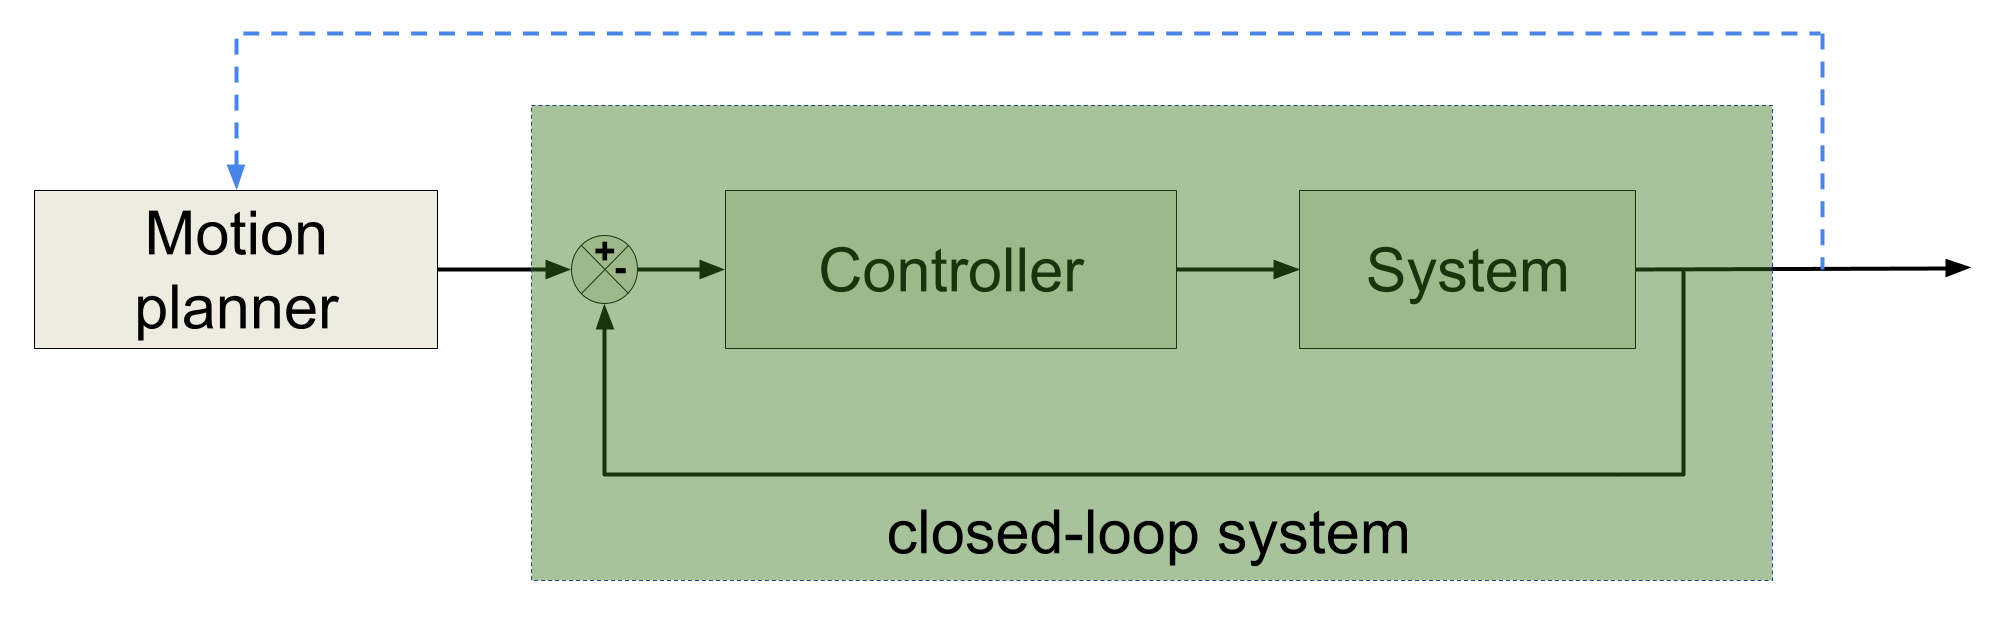
\includegraphics[width=0.9\linewidth]{figures/intro/control-aware.png} 
    \caption{Illustration of the control-aware motion planning strategy.
    It relies on the closed-loop system simulation (green) at the offline motion planning level (gray).}%
    \label{fig:ca_strat}%
  \end{figure}

\section{Thesis Outline}

This manuscript begins with a literature review in Chapter~\ref{chap:related_work}, providing an overview of the current state of the art. 
It initially focuses on decoupled approaches to robust motion planning, starting with path finding methods and progressing to kinodynamic planning paired with robust control strategies.
The review then continues to unified approaches, presenting robust motion planning methods that address uncertainty, as well as control-aware planning techniques. 
The chapter concludes with a focus on unified robust control-aware motion planning approaches, which form the main topic of interest.

Chapter~\ref{chap:models} introduces the \emph{closed-loop sensitivity} concept and present how this concept can be leveraged to derive the so-called uncertainty tubes.
These uncertainty tubes are later employed in this thesis to impose robust constraints on systems while accounting for parametric uncertainties.
Then, this chapter presents the quadrotor and differential drive robot models considered in this thesis, along with their respective controllers and local planning techniques used for generating reference trajectories.

The first contribution of this thesis is then introduced in Chapter~\ref{chap:samp}.
It presents the general method for integrating sensitivity-based uncertainty tubes into sampling-based planners to create various sensitivity-aware motion planner variants.
Furthermore, this chapter emphasizing the generation of sensitivity-optimal trajectories in global context.
Initial simulation results, using the models introduced in Chapter~\ref{chap:models}, highlight that computing uncertainty tubes become a bottleneck for sampling-based methods.
To address this, a more efficient variant is proposed, leveraging a lazy collision-checking approach to reduce the frequency of uncertainty tube computations.

Chapter~\ref{chap:NN} introduces the second major contribution of this thesis, which leverages the structural similarities between ordinary differential equations and recurrent neural network cells to accelerate the computation of sensitivity-based uncertainty tubes. 
A dataset generation method, based on sampling-based principle, is proposed and applied to the models discussed in Chapter~\ref{chap:models}. 
The method achieves an optimal balance between inference time and accuracy, making it highly effective for motion planning and showcasing the efficiency of the approach.

Chapter~\ref{chap:sampNN} aims to integrate the sensitivity-aware motion planning variants introduced in Chapter~\ref{chap:samp} with the deep learning approach detailed in Chapter~\ref{chap:NN}, resulting in a more efficient version of the sensitivity-aware motion planner variants.
Furthermore, while the previous chapters solely focus on generating robust and sensitivity-optimized trajectories, this chapter emphasizes the generation of task-specific accurate trajectories.
The effectiveness of this contribution is finally demonstrated through experimental validation on two challenging scenarios requiring high robustness and accuracy.

Finally, Chapter~\ref{chap:concl} presents an overall conclusion that summarizes the contributions of this thesis along with their limitations.
Additionally, several perspectives are outlined to improve the generalizability of the proposed approach.

\section{Thesis Contributions}

The work conducted throughout this thesis led to the following publications in international peer-reviewed conferences and letters. 

~\cite{cSAMP} Wasiela, S., Giordano, P. R., Cortés, J., and Simeon, T. (2023, May). "A sensitivity-aware motion planner (samp) to generate intrinsically-robust trajectories." In IEEE International Conference on Robotics and Automation (ICRA) (pp. 12707-12713).

~\cite{cECAI}: Wasiela, S., Bouhsain, S. A., Cognetti, M., Cortés, J., and Simeon, T. (2024, October). "Learned Uncertainty Tubes via Recurrent Neural Networks for Planning Robust Robot Motions." In 27th European Conference on Artificial Intelligence (ECAI) (pp. 4385-4392).

~\cite{cRAL}: Wasiela, S., Cognetti, M., Giordano, P. R., Cortés, J., and Simeon, T. (2024). "Robust Motion Planning with Accuracy Optimization based on Learned Sensitivity Metrics." In IEEE Robotics and Automation Letters (RA-L).

Furthermore, all implementations presented and used in this thesis are available at: \href{https://gitlab.laas.fr/CAMP}{https://gitlab.laas.fr/CAMP}.
% \cleardoublepage
% \newpage 
% \ % The empty page
% \newpage
\chapter{Related work}\label{chap:related_work}
\markboth{Related work}{}% To set left/right header
% \localtableofcontents

This chapter provides an overview of the related work on the key concepts that this thesis builds upon and compares with.

\section{Motion planning}

\subsection{Path planning}

This subsection provides an overview of various path planning approaches. 
For a more detailed survey, please refer to~\cite{cLavalle, cKavraki, cFrazzoli}.
The path planning problem focuses on finding a collision-free and/or optimal path between two configurations: a starting configuration and a goal configuration. 
The work of~\cite{cConfigSpace} introduced the configuration space concept as a general framework for planning motions in arbitrary kinematic systems.
This idea provided a solid foundation for the field and, as noted in~\cite{cSpatialPlan}, formally established the motion planning problem as the task of finding a path within the configuration space.

However, planning motion in the configuration space poses significant challenges due to the problem computational complexity. 
A key stone in addressing this issue is the introduction of artificial potential fields~\cite{cAPF}, which create a repulsive force field around obstacles and an attractive force field toward the target.
However, although this strategy has proven to be efficient, it sacrifices guarantees such as algorithm completeness and optimality.

Another common approach to the path planning problem involves search-based techniques. 
These methods operate on a discrete representation of the configuration space, where vertices correspond to a finite set of robot configurations, and edges represent possible transitions between these configurations.
The desired path is found by performing a search for a minimum-cost path in such a graph using Dijkstra algorithm~\cite{cDijk}. 

Advances in computational techniques have enabled the development of a new class of algorithms, commonly referred to as sampling-based planners that allow to generate global motion plans.
A key contribution of the domain is the work of~\cite{cLatombe}, which improves the aforementioned potential fields approach by integrating a random walk mechanism, thus guaranteeing the probabilistic completeness of the algorithm.
Sampling-based planners are divided in two main categories: graph-based planners and tree-based planners.

Graph-based sampling-based planners, such as \gls{prm}~\cite{cPRM}, generate a roadmap by sampling configurations in the free space and connecting them with feasible paths. 
The technique involves a graph building phase and a query phase.
The graph is first built by randomly sampling configurations (denoted nodes) in the robot configuration space.
Each sampled configuration is checked for collisions with obstacles.
For each collision-free node, the planner attempts to connect it to nearby free configurations by creating edges between them.  
The edges are valid if the path connecting the two configurations is collision-free.
This procedure typically involves a notion of neighborhood that is space-dependent and generally increases as the dimensionality of the space grows.
Once the graph is built, a graph search query is performed to compute the desired path, using graph search techniques such as Dijkstra algorithm~\cite{cDijk} or A*~\cite{cA*}.

The other planner family among sampling-based planners are tree-based planners such as the well-known \gls{rrt}~\cite{cRRT}.
This algorithm generates a tree starting from an initial configuration.
At each iteration, a new configuration is sampled $q^{rand}$.
It's nearest neighbor among the existing tree nodes is found $q^{near}$, and then an extension is attempt starting from $q^{near}$ toward $q^{rand}$ leading to a new configuration $q^{new}$.
If the extension is collision free, the new configuration is added to the tree as a new node with an edge connecting the two nodes.

Therefore, sampling-based motion planners have become one of the most widely used strategy for generating global motion paths in the presence of obstacles, due to their efficiency in handling complex and high-dimensional configuration spaces, as well as their completeness guarantee.
Advances in sampling-based planners have then focused on generating feasible and cost-effective paths through various strategies, such as the transition-based approach~\cite{cTRRT}. 
These strategies often achieve asymptotic optimality by employing optimal connection procedures during the tree or graph construction process~\cite{cRRTstar, cTRRTstar, cFMT}.
Research on sampling-based planners has expanded into various areas, such as developing suitable sampling strategies~\cite{cSampling}, exploring lazy collision checking approaches~\cite{cLazy1}, extending to the molecular domain~\cite{cMolecular}, and more.

The aforementioned sampling-based methods are generally referred to as global planning methods, as they rely on local planning techniques to generate the edges that connect the sampled configurations.
Such local planning methods are not considered global, as they do not address the entire motion planning problem. 
A local planner is typically fast; however, the generated path may not fully satisfy the problem constraints (e.g., it could result in collisions).
Traditional local strategies typically involve path segments, but local planners often need to account for additional constraints.
For example, significant work has been done to enforce kinematic constraints on these local plans, ensuring the kinematic feasibility of the resulting global paths.
Such work includes, for example, Dubins path generation~\cite{cDubins}, which enables connecting two configurations under forward motion constraints and curvature constraints for car-like robots. 
The Reeds-Shepp method~\cite{cReeds} extends this local path generation procedure to car-like robots capable of moving both forward and backward.

\subsection{Kinodynamic planning}

While the aforementioned path finding methods focus on generating a route between two robot configurations, they do not address the problem on how the robot should move along this route over time.
Additionally, path planning does not account for the robot dynamic constraints, such as maximum velocity and acceleration. 
The problem of generating motion plans that consider both kinematic constraints (e.g., turning radius) and dynamic constraints, ensuring the plans are physically executable, is known as kinodynamic motion planning.
Therefore, the kinodynamic problem extends beyond searching in the robot configuration space by considering its entire state space.

\subsubsection{Local planners}

Local planners, or steering methods, focus on generating feasible motion between two states while respecting kinematic and dynamic constraints. 
They are often used as building blocks in global kinodynamic planners. 

A common approach to generating smooth trajectories between robot states is to solve a two-point \gls{bvp} using polynomial-based methods, such as splines, which are widely employed for trajectory interpolation. 
For instance, the kino-splines local planner proposed in~\cite{cKino} leverages system differential flatness, ensuring the creation of continuous and differentiable trajectories up to the 4th order by employing a bang-bang snap control strategy. 
The resulting trajectories respect kinodynamic constraints up to the jerk level, enabling time-optimal connections between two given states. 
Another example is the minimum snap trajectory generation method~\cite{cMinimumSnap}, which contrasts with the bang-bang snap strategy of kino-splines. 
Also based on system differential flatness, this approach formulates an optimization problem that minimizes the integral of a weighted combination of squared position snap and squared yaw acceleration.
It ensures continuity between trajectory segments, satisfies kinematic conditions at the start and end of the motion, and respects actuation limits.

While the local planners mentioned earlier primarily focus on enforcing kinodynamic constraints, Bézier curve-based planners~\cite{cBezier,cBezier2} offer additional benefits due to their inherent smoothness, and their convex hull property.
Their convex hull property ensures that the trajectory remains within the convex hull of its control points. 
This simplifies collision detection, as it guarantees that if the convex hull is free of obstacles, the entire trajectory will be too. 
Additionally, adjusting control points affects only a localized portion of the trajectory, allowing precise modifications without affecting the entire trajectory. 
This approach is particularly useful in environments where efficient collision detection is crucial.
Furthermore, its smoothness also naturally accommodates velocity, acceleration, and higher-order dynamic constraints, making it suitable for kinodynamic motion planning in various robotic systems. 

Another powerful method is \gls{chomp}~\cite{cCHOMP}, which formulates trajectory generation as an optimization problem starting from an initial trajectory as guess. 
The cost function in \myglsentry{chomp} typically balances smoothness and obstacle avoidance.
Smoothness is ensured by penalizing higher derivatives of the trajectory, while obstacle avoidance is achieved through the use of a signed distance field. 
\myglsentry{chomp} can incorporate dynamic and kinematic constraints, such as joint limits and velocity bounds, which are important for kinodynamic planning. 
Using gradient-based optimization, \myglsentry{chomp} iteratively refines the initial trajectory, ensuring that it satisfies all constraints while minimizing the cost function. 
While effective in high-dimensional or cluttered environments, \myglsentry{chomp} does require a good initial trajectory and can struggle in environments with non-convex obstacles.

While \myglsentry{chomp} can handle differentiable cost function due its gradient-based optimization, the \gls{stomp} algorithm~\cite{cSTOMP} is designed to optimize non-differentiable cost functions. 
\myglsentry{stomp} iteratively improves trajectories by introducing small perturbations to the initial guess, evaluating the resulting costs, and updating the trajectory based on the best-performing samples. 
This process also accounts for kinodynamic constraints and obstacle avoidance by adding state cost penalty in the cost function formulation.
While \myglsentry{stomp} is computationally more expensive than \myglsentry{chomp} as it relies on several sampling-based rollouts, its ability to handle more complex cost functions and find better solutions in challenging environments makes it highly versatile for kinodynamic motion planning.

\subsubsection{Forward propagation}\label{sec:forwardplanning}

Global sampling-based motion planners can generate globally kinodynamically feasible trajectories by leveraging the aforementioned local planners to connect their sampled state.
However, such local planners may not be available for every system.
Therefore, algorithms were developed to bypass this need by performing dynamic system forward propagation instead of solving a complex \myglsentry{bvp}.

Kinodynamic motion planners, such as Kinodynamic RRT~\cite{cKinoRRT} and \gls{sst}~\cite{cSST}, are designed to address the challenges of planning for robots with complex dynamics without relying on a local planner. 
These methods utilize system forward dynamic propagation by sampling control inputs and propagation time. 
Starting from an initial robot state, the system dynamics are integrated in an open-loop manner to propagate the state, allowing the planner to account for both the robot kinematic limitations and its dynamic behavior. 
This approach ensures that the generated paths are collision-free and physically executable while eliminating the need for local planners.

\section{Planning under uncertainty}

While the previous section focused on motion planning algorithms that can deal with kinodynamic constraints of various robot, none of them consider the unavoidable presence of uncertainties (e.g. external disturbances, sensor noise, model parameter mismatches, etc.).

A common approach to managing uncertainties is to compensate for them in real-time using robust controllers, such as H-infinity or \gls{lpv} methods.
However, these methods often encounter difficulties in maintaining robustness when applied to non-robust reference trajectories, due to their inherently local nature.
Additionally, they struggle to achieve global optimality and performance, which are typically better addressed by global planning approaches.
Therefore, considerable research has focused on designing motion planning algorithms that incorporate uncertainty into the trajectory generation process, with the goal of producing robust and feasible plans.

A seminal contribution to the field is the \gls{lmt} framework~\cite{cLMT}, which addresses the challenge of computing compliant motion strategies in the presence of sensor uncertainties and inaccuracies in robot movement. 
This approach focuses on developing fine-motion strategies, which involve incrementally generating sequences of robot movements that account for inaccuracies in both the robot state and the sensed environment. 
The authors consider the robot kinematic constraints and sources of error, such as sensor discrepancies or movement inaccuracies.
By ensuring that the robot motions remain collision-free and adaptable to these uncertainties, the framework aims to achieve robustness in real-world tasks.
However, a bottleneck of the method is its high computational cost.

By leveraging the probabilistic robotic concept~\cite{cProbaRobotic}, approaches such as \gls{pomdp} or, in general, the class of “planning in belief spaces” approaches, are another alternative for providing a principled and general planning framework for dealing with uncertainty.
They use stochastic uncertainty propagation functions, to minimize the uncertainty along the trajectory to the desired target~\cite{cUncertaintyPOMDP,cNavigationPOMPDP}. 
\myglsentry{pomdp} model sequential decision-making in environments with uncertainty, considering both actions taken by the agent and the uncertain nature of observations and transitions.
The proposed frameworks have the advantage of being adaptable to a wide range of non-trivial robot models, with non-Gaussian processes and observation models for trajectory planning with minimum uncertainty.
However, these methods still suffer from computational bottleneck when dealing with high dimensional problems.

When probability distributions over uncertain variables are available, chance-constrained motion planning can be used to generate plans that satisfy probabilistic constraints~\cite{cChance1,cChance2,cChance3}. 
These constraints ensure that specific conditions, such as safety or feasibility, are met with a certain probability. 
Typically, a chance constraint is incorporated into an optimization problem, where the objective (e.g., minimizing cost or maximizing reward) is optimized while ensuring that the constraint holds with a high probability (e.g. ensuring that a robot avoids obstacles with 95\% probability).

Particle-based methods such as Particle RRT~\cite{cParticleRRT} or RRT-SALM~\cite{cSlamRRT}, use particle filters to model uncertainty. 
Rather than relying on a single robot state, these algorithms represent the robot state as a set of particles, each corresponding to a possible uncertain state. 
The particles are propagated through the environment according to the system dynamic, and the tree is expanded by sampling from these particles.

The problem of generating open-loop trajectories with minimum state sensitivity has been recently addressed in~\cite{cSensi1} and further expanded upon in~\cite{cSensi2}. 
This later work introduces a method for generating robust trajectories using an open-loop optimization routine that accounts for deviations in model parameters. 
In contrast to the aforementioned probabilistic approaches, this framework operates under the assumption of accurate models and demonstrates that minimizing first-order sensitivities leads to reduced deviations from the nominal state when model parameters are imperfect.

\section{Control-aware motion planning}

The algorithms presented so far have been designed to handle kinodynamic constraints and/or ensure robustness against various uncertainties.
However, none of them typically consider the inevitable presence of a feedback controller responsible for executing the generated trajectories. 
This controller might deviate from the planned trajectory to address uncertainties and disturbances, which can quickly compromise feasibility and optimality of the plan.
It is important to note that kinodynamic approaches relying on system dynamics forward propagation, as discussed in Section~\ref{sec:forwardplanning}, do not incorporate feedback actions.
Instead, they directly sample in the control input space, resulting in an open-loop propagation strategy.

The idea of merging planning with control for generating “robust planners” or more “global controllers” for dealing with the robustness problem in a more comprehensive way is however not completely novel in the robotics community.

Work has been carried out on the control community side to propose ``less local'' controllers, resulting in the popular \gls{mpc} technique~\cite{cMPC} that iteratively replans an optimal (and feasible) trajectory with a feedback from the current robot state (that may deviate from the desired one because of disturbances/uncertainties). 
This method enables fast computation of locally optimal trajectories while incorporating the controller feedback action. 
However, due to its inherently local nature, the \myglsentry{mpc} approach can become trapped in local minima with respect to cost or obstacles. 
It often lacks guarantees of completeness and relies heavily on an accurate robot model, without explicitly accounting for uncertainties.

The LQR-Trees method~\cite{cLQRTrees} address the problem of computing motion plans that are stabilizable.

MPC and control-aware from M Tognon and LQR trees

\section{Robust control-aware motion planning}

one should guarantee safe operation for all uncertainty realizations within these bounds taking into account for the presence of a feedback controller. This task is referred to as robust control-aware motion planning (or robust feedback motion planning).

\subsection{Tube MPC}

\subsection{FaSTrack}

\subsection{Funnel library}

\subsection{Contraction theory}

\subsection{Randomized uncertainty propagation}

\subsection{CLosed-loop Sensitivity}

\section{Summary}
% \cleardoublepage
% \newpage 
% \ % The empty page
% \newpage
\chapter{Preliminaries}\label{chap:models}
\markboth{Preliminaries}{}% To set left/right header
\localtableofcontents \newpage

This chapter introduces the notion of \emph{closed-loop sensitivity}, which forms a key foundation of this thesis.
This concept quantifies how variations of some model parameters (supposed to be uncertain) affect the evolution of the system in closed-loop, i.e., by also taking into account any controller chosen for executing the task.
Then, it is presented how this sensitivity notion can be leveraged to derive \emph{uncertainty tubes} that bounds the system evolution both in the \emph{input} and \emph{state} spaces.
These tubes are subsequently used to enforce robust constraints within the several motion planning algorithms presented in this thesis.
Finally, the quadrotor and differential drive robot models used in this manuscript are introduced.

\section{Closed-loop sensitivity}\label{sec:sensi_and_tubes}

\subsection{Definition}\label{sec:sensi}

Consider an arbitrary dynamic system with a set of uncertain parameters $\p \in \mathbb{R}^{n_p}$ (i.e. parameters that are difficult to model).
The system dynamic can be described using the following set of \gls{odes}:
\begin{equation}\label{eq:dyna}
    \dot{\q}=\f(\q,\,\u,\,\p), \quad \q(t_0)=\q_{0},
\end{equation}
where $\q\in \mathbb{R}^{n_{q}}$ is the system state vector and $\u\in \mathbb{R}^{n_{u}}$ is the control input vector.
Also, assume the presence of a controller $\boldmu$ of any form whose aim is to track a \emph{desired trajectory} $\q_d(t)$ such that:
\begin{equation}\label{eq:ctrl}
     \left \{
     \begin{array}{l l}
          \dot{\bxi} = \g(\bxi,\,\q,\,\q_d,\,\p_n,\,\k_c,\,t), \quad \bxi(t_0)=\bxi_{0}, \\
          \u=\boldmu(\bxi,\,\q,\,\q_d,\,\p_n,\,\k_c,\,t), 
   \end{array} 
   \right .
\end{equation}
where $\bxi\in \mathbb{R}^{n_{\xi}}$ are the internal states of the controller (e.g., an integral action), $\k_{c}\in \mathbb{R}^{n_{k}}$ the controller gains, and $\p_{n}\in{\mathbb{R}^{n_{p}}}$ is the vector of "nominal" system parameters used in the control loop, i.e. the estimated nominal values of $\p$.
Note that the controller operates based on the nominal parameters $\p_{n}$, while the actual parameters $\p$, which influence the system, remain unknown and cannot be determined.
It is also important to note that, in this thesis, the system state $\q$ is assumed to be perfectly known, as no sensor models are considered.
Consequently, the simulations and subsequent sensitivity computations are performed using the true system state $\q$, rather than the usual estimation of this state $\hat{\q}$.

In line with the previous definitions, the following sections of this thesis will then differentiate between three types of state vectors of key importance:
\begin{enumerate}
  \item $\q_d$: The \emph{desired} system state vector which refers to the desired values of the controllable system states. 
  This state vector is typically the output of a motion planner. Note that the dimension of this vector may differ from that of the real system because the vector represents a simplified or abstracted model, which might omit certain physical aspects or constraints that are present in the actual system, particularly in the case of under-actuated systems, where not all degrees of freedom are controlled.
  \item $\q_n$: The \emph{nominal} system state vector which represents the real state values of the system during the execution under nominal parameters (i.e. when the uncertain system parameters $\p$ perfectly match the parameter values used in the control loop $\p_n$). 
  A distinction is made between the nominal states and the desired states, as they are generally not equal due to factors such as controller settings (e.g. overshooting behavior).
  \item $\q$: The \emph{uncertain} system state vector which refers to the behavior of the system when the values of real parameters are taken into account.
\end{enumerate}
Note that the same notations apply to the control input vector as well (e.g., $\u_n$ represents the "nominal" control input values, i.e., when $\p=\p_n$).

It is possible to quantify how the presence of uncertain parameters (i.e. when the real system parameters $\p$ deviate from the nominal value $\p_n$ used in the control loop) affects the evolution of $\q(t)$ and $\u(t)$ according to the following matrices:
\begin{equation}\label{eq:sensi}
  \bPi(t)=\left.\frac{\partial \q(t)}{\partial \p}\right|_{\p=\p_n} \quad\quad \bTheta(t)=\left.\frac{\partial \u(t)}{\partial \p}\right|_{\p=\p_n}
\end{equation}
where $\bPi(t)\in \mathbb{R}^{n_q \times n_p}$ and $\bTheta(t)\in \mathbb{R}^{n_u \times n_p}$ are respectively defined in~\cite{cPi,cTh} as the \emph{state-sensitivity matrix} and the \emph{input-sensitivity matrix}.
A closed-form expression for Equation~(\ref{eq:sensi}) is, in general, not available. 
However, as shown in~\cite{cPi,cTh}, their evolution in time can be computed by differentiating Equation~(\ref{eq:sensi}) according to the following set of \myglsentry{odes}:
\begin{equation}\label{eq:dyna_sensi}
  \left \{
  \begin{array}{l l l}
       \dot{\bPi}(t) = \boldsymbol{\frac{\partial{f}}{\partial{q}}}\bPi+ \boldsymbol{\frac{\partial{f}}{\partial{u}}}\bTheta+ \boldsymbol{\frac{\partial{f}}{\partial{p}}}, \quad \bPi(t_0)=\bPi_0, \\
       \dot{\bPi}_{\xi}(t) = \boldsymbol{\frac{\partial{g}}{\partial{q}}}\bPi+ \boldsymbol{\frac{\partial{g}}{\partial{\xi}}}\bPi_{\xi}, \quad \bPi_{\xi}(t_0)=\bPi_{\xi0}, \\
       \bTheta(t) = \boldsymbol{\frac{\partial{h}}{\partial{q}}}\bPi+ \boldsymbol{\frac{\partial{h}}{\partial{\xi}}}\bPi_{\xi} 
  \end{array}
  \right .
\end{equation}
where $\bPixi(t)\in \mathbb{R}^{n_{\xi} \times n_p}$ represents the \emph{internal state sensitivity} matrix.

Now that the sensitivity matrices are defined, one can optimize the desired trajectory s.t. a norm of these matrices is minimized (see~\cite{cPi,cTh}). 
This optimization produces a trajectory s.t. the closed-loop evolution of $\q(t)$ and $\u(t)$ closely matches their evolutions in the nominal case $\q_n(t)$ and $\u_n(t)$.

\subsection{Tube computation}\label{sec:tubes}

\begin{figure} [t]
  \centering
  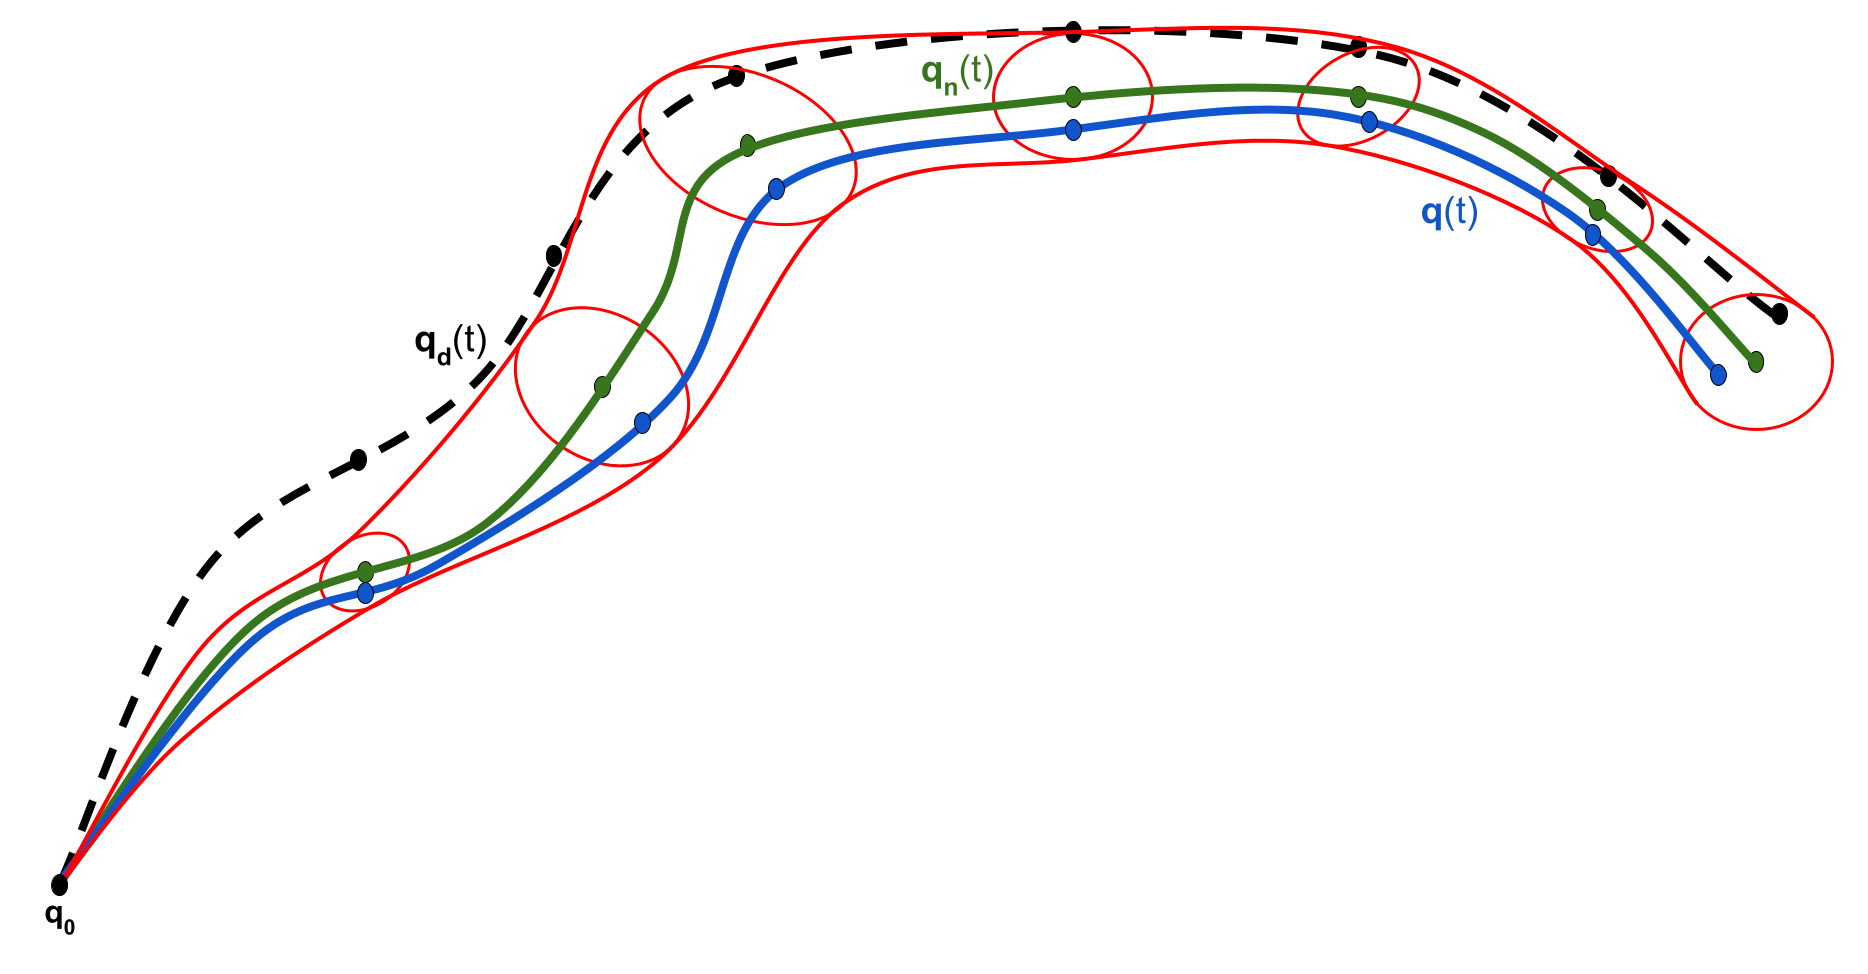
\includegraphics[width=0.8\linewidth]{figures/models/tubes.png} 
  \caption{Illustration of the uncertainty tube (red) and a perturbed trajectory $\q(t)$ (blue), centered around the nominal trajectory $\q_n(t)$ (green), which results from following the reference trajectory $\q_d(t)$ (dashed black).}%
  \label{fig:tubes}%
\end{figure}

\begin{figure} [t]
  \centering
  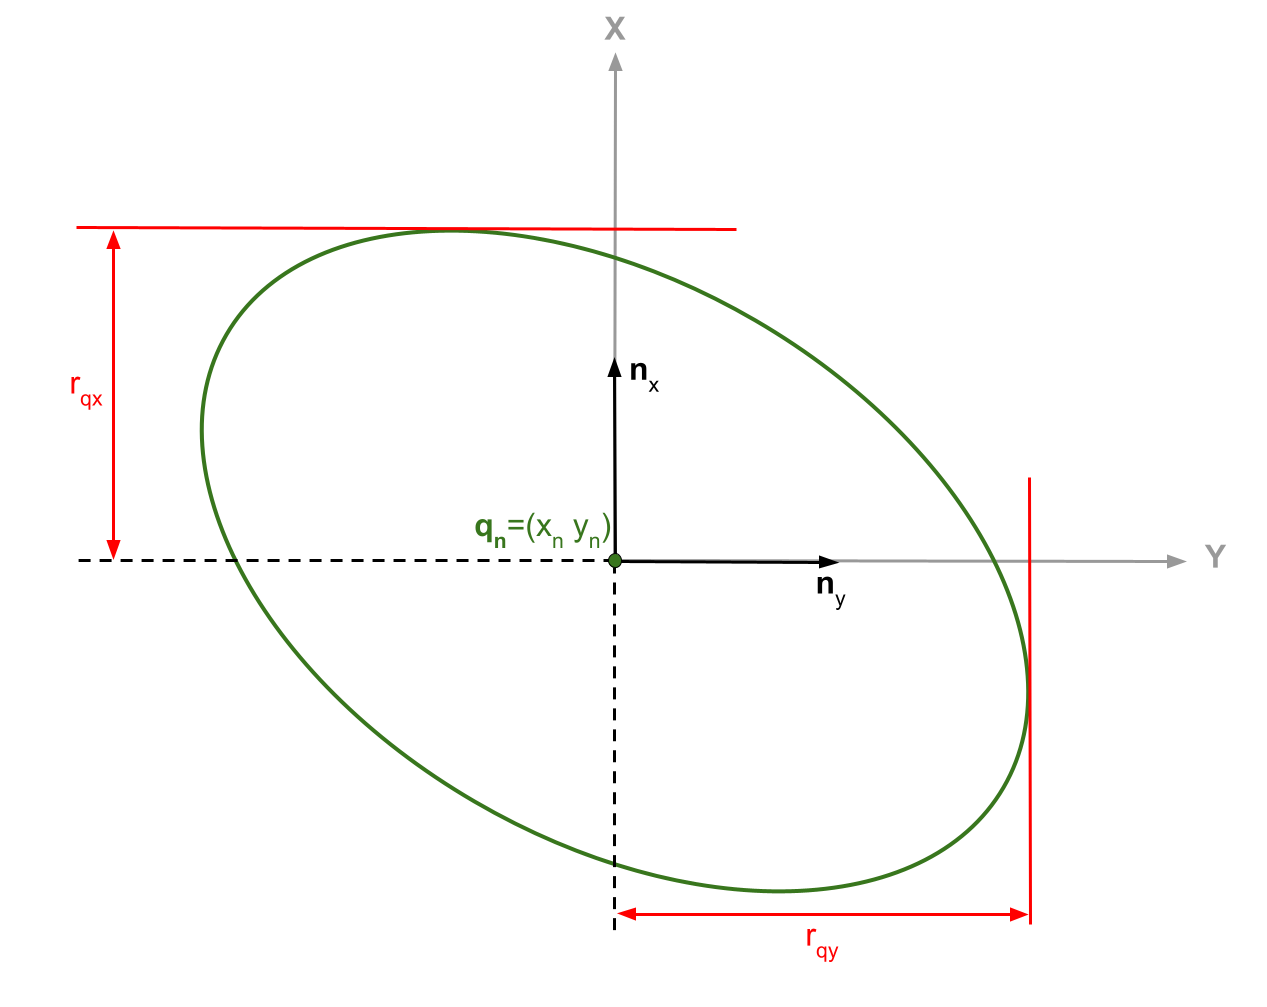
\includegraphics[width=0.6\linewidth]{figures/models/radius.png} 
  \caption{2D representation of an uncertainty ellipse (green) in the x-y state space centered at $\q_n$, along with the tube radius (red) that illustrates the worst-case deviations along each state space components.}%
  \label{fig:ellips_radius}%
\end{figure}

Another important feature of the sensitivity matrices is that it is possible to derive the so-called \emph{uncertainty tubes}, that bounds the closed-loop system trajectory $\q(t)$/$\u(t)$ around its nominal trajectory $\q_n(t)$/$\u_n(t)$ as shown in~\cite{cTube} and illustrated in Figure~\ref{fig:tubes}.
The rest of this section shows how to establish such bounds around the nominal state trajectory $\q_n(t)$ by focusing solely on the state-sensitivity matrix $\bPi(t)$ for clarity. 
However, it is important to note that the same procedure can also be applied to compute bounds around the nominal input trajectory $\u_n(t)$ by leveraging the input-sensitivity matrix $\bTheta(t)$.

Assume that for each uncertain parameter $p_{i}, i \in [1, n_p]$ in $\p$, we have a bounded parameter deviation $\delta p_i \in \mathbb{R}$ s.t. 
\begin{equation*}
  \forall i \in [1, n_p] ,p_i \in [p_{n_i}-\delta p_i, p_{n_i}+\delta p_i].
\end{equation*}
Such deviations can be mapped into the parameter space by mean of the following ellipsoid
\begin{equation}\label{eq:p_ellipsoid}
  \Delta\p^T \bW^{-1} \Delta\p \leq 1,
\end{equation}
where $\bW$ is the following diagonal weight matrix
\begin{equation*}
  \bW = \begin{bmatrix}
    \delta p_1^2 & 0 & \cdots & 0 \\
    0 & \delta p_2^2 & \cdots & 0 \\
    \vdots & \vdots & \ddots & \vdots \\
    0 & 0 & \cdots & \delta p_{n_p}^2
    \end{bmatrix} \in \mathbb{R}^{n_p \times n_p}.
\end{equation*}

Assuming small parameters variations (i.e. small $\delta \p$) it is possible to perform a first-order approximation around the nominal trajectory $\q_n(t)$ to obtain 
\begin{equation}\label{eq:approx}
  \Delta\q(t) =  \q(t) - \q_n(t) \approx \bPi(t) \Delta\p.
\end{equation}

Without loss of generality, for a well-chosen $\delta \p$ s.t. Equation~(\ref{eq:approx}) holds, ~\cite{cTube} has shown how to map the parameters ellipsoid from Equation~(\ref{eq:p_ellipsoid}) in the system state space in order to obtain the corresponding uncertainty ellipsoid
\begin{equation}\label{eq:q_ellipsoid}
  \Delta\q(t)^T (\bPi(t) \bW \bPi(t)^T)^\dag \Delta\q(t) \leq 1.
\end{equation}
However, it is important to note that the ellipsoid axes are in general not aligned with the canonical basis of the state space.
This implies that computing the deviation of each state component $q_i(t)$ is not straightforward, as direct use of the ellipsoid semi-axes length is not possible.
%  and the direction of interest may not belong to the range of the ellipsoid.

Nevertheless, it has been shown in~\cite{cTube} how to evaluate the radius $r_{q,i}(t)\geq 0$ of the perturbed tubes along the $i$-th component of the state $q_i(t)$ by mean of the following projection:
\begin{equation}\label{eq:radius}
  r_{q,i}(t) =  \sqrt{\boldsymbol{n_i}^{T} \boldsymbol{K_{\Pi}}(t) \boldsymbol{n_i}},
\end{equation}
where $\boldsymbol{n}_i$ is the unit-norm vector of the $i$-th state space component, and $\boldsymbol{K_{\Pi}}(t) = \boldsymbol{\Pi}(t)\boldsymbol{W}\boldsymbol{\Pi}(t)^T$ is the kernel matrix of Equation~(\ref{eq:q_ellipsoid}).
It is important to note that the radius along the $i$-th component represents the maximum possible deviation in that direction and does not directly correspond to the semi-axes of the uncertainty ellipsoid as depicted in Figure~\ref{fig:ellips_radius}.

The quantities $r_{q,i}(t)$ can then be used to bound components of the states $\q(t)$ or inputs $\u(t)$ over time.
For example, letting $q_{n,i}(t)$ the behavior of the $i$-th state component in the nominal case (non-perturbed case), the so-called \emph{uncertainty tube} along this component is defined s.t.:
\begin{equation}\label{eq:bounds_q}
  q_{n,i}(t) - r_{q,i}(t) \leq q_i(t) \leq q_{n,i}(t) + r_{q,i}(t),
\end{equation}
for a perturbed state $q_i(t)$, and an analogous derivation is also possible for the control inputs $\u(t)$.

Finally, it is important to underline that since the uncertainty tube radii depend on the state sensitivity $\boldsymbol{\Pi}(t)$, it is necessary to solve the set of \myglsentry{odes} represented by Equation~(\ref{eq:dyna}), Equation~(\ref{eq:ctrl}), and Equation~(\ref{eq:dyna_sensi}) beforehand.
Additionally, note how, in general, the tube radius does not necessarily increase monotonically due to the influence of feedback action as illustrated in Figure~\ref{fig:tubes}, despite the cumulative effect of uncertainties over time. 

\section{Models considered in this thesis}

To demonstrate the versatility of the approaches proposed in this thesis across various robots and controllers, a quadrotor and a differential drive robot are considered in this manuscript, along with two distinct controllers and interpolation methods, which are detailed in the following sections.

\subsection{Quadrotor robot} \label{sec:quad_model}

\subsubsection{Dynamic model}

\begin{figure} [t]
    \centering
    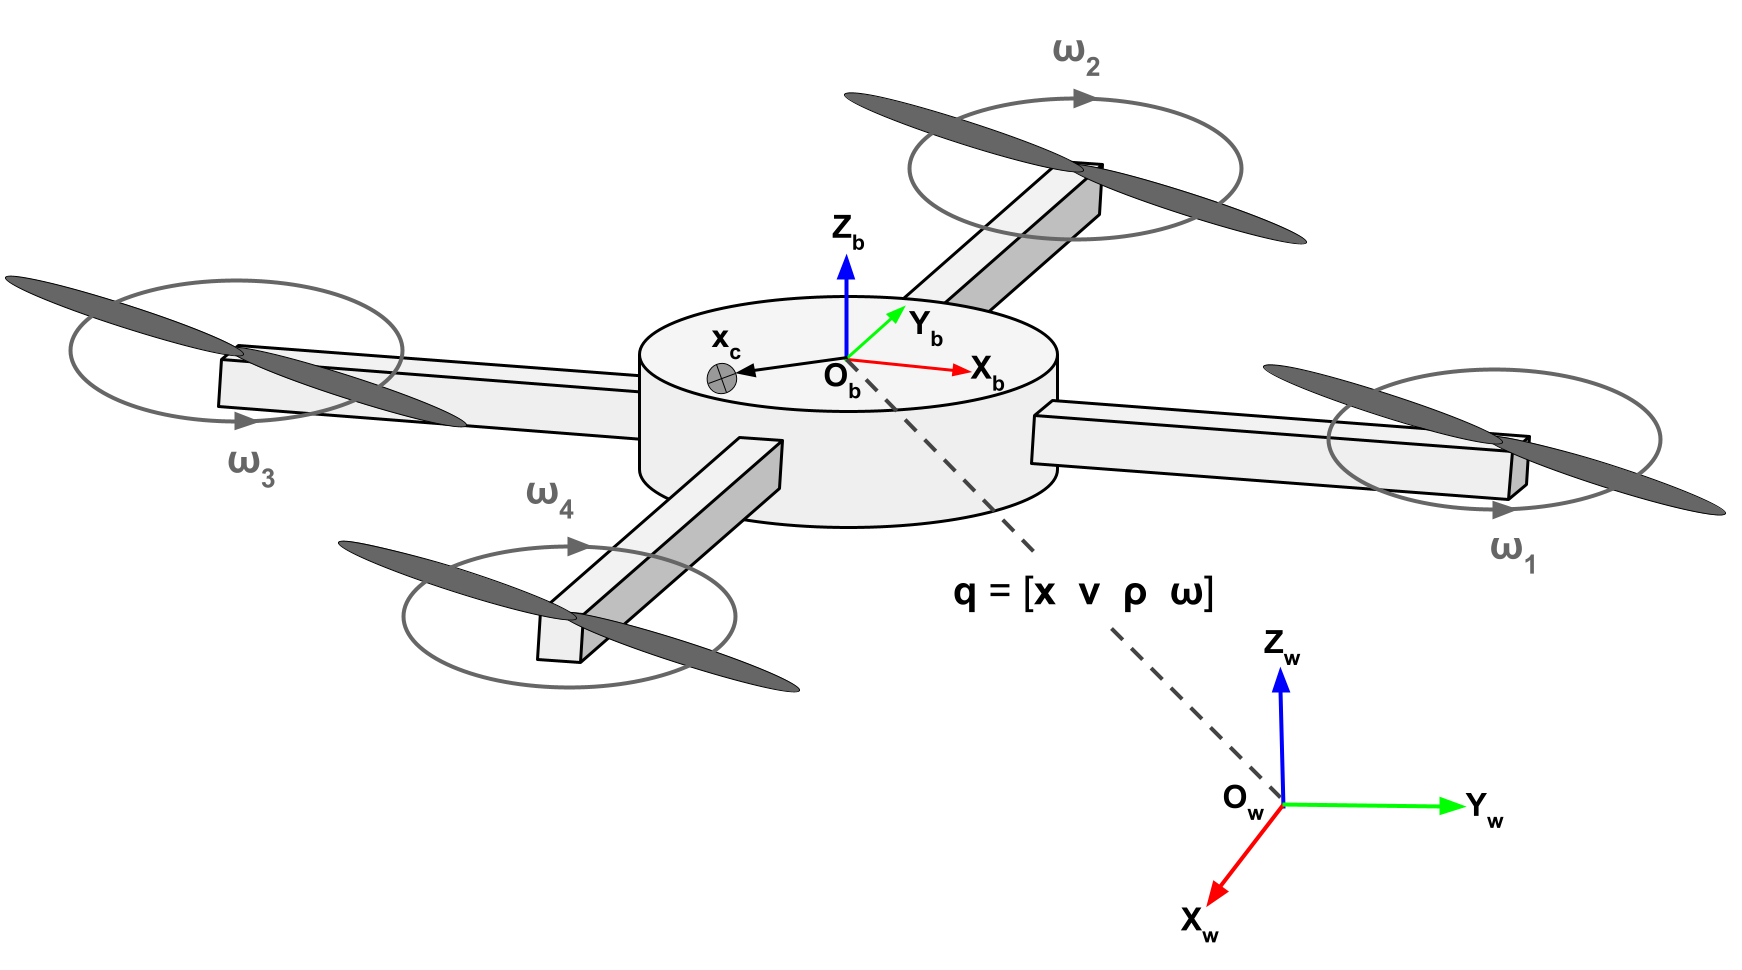
\includegraphics[width=0.8\linewidth]{figures/models/drone.png} 
    \caption{Quadrotor robot representation with a shift in the center of mass.}%
    \label{fig:quad}%
\end{figure}

Let the ENU (East North Up) world frame be defined as $F_W \allowbreak = \allowbreak \{O_W, \allowbreak X_W, \allowbreak Y_W, \allowbreak Z_W\}$ and $F_B = \allowbreak\{O_B, \allowbreak X_B, \allowbreak Y_B, \allowbreak Z_B\}$ be the quadrotor body frame attached to its geometric center ($O_B$).
The state of the quadrotor is defined as $\boldsymbol{q} = [\boldsymbol{x}  \, \boldsymbol{v} \, \boldsymbol{\rho} \, \boldsymbol{\omega}]$ where $\boldsymbol{x} = [x \, y \,z] \in \mathbb{R}^{3}$ and $\boldsymbol{v} = [v_x \, v_y \,v_z] \in \mathbb{R}^{3}$ are respectively the position and linear velocity vector of $O_B$ expressed in $F_W$. The body orientation w.r.t. $F_W$ is represented by the unitary quaternion $\boldsymbol{\rho}$ and its angular velocity as $\boldsymbol{\omega} = [\omega_x \, \omega_y \, \omega_z] \in \mathbb{R}^{3}$. 
Finally, let $\boldsymbol{R(\rho)}$ be the rotation matrix associated to $\boldsymbol{\rho}$.

Let the control input vector $\u = [\omega_{1}^2 \, \omega_{2}^2 \, \omega_{3}^2 \, \omega_{4}^2]^T$ represents the squared rotor speeds. 
The vector $\u$ is related to the total propeller thrust $f$ and torques $\boldsymbol{\tau}$ by mean of a standard allocation matrix $\boldsymbol{T}$ s.t.
\begin{equation}\label{eq:alloc_mat}
  \begin{bmatrix}
    f \\
    \boldsymbol{\tau}
    \end{bmatrix} = \boldsymbol{T}(l, k_f, k_{\tau}) \u,
\end{equation}
where $k_f$ and $k_{\tau}$ refer to the thrust and drag coefficients of the propellers respectively, and $l$ stands for the quadrotor arm length.
Also, consider that the \gls{com} is displaced from the robot geometric center of an offset $\boldsymbol{x_{c}} = [x_{cx} \, x_{cy} \, x_{cz}]$ expressed in $F_B$ as depicted in Figure~\ref{fig:quad}. 
This displacement can occur due to onboard sensors, the presence of a payload, or other factors.
Under this consideration and according to Newton's second law, the total force ($\boldsymbol{f_{tot}}$) and torque ($\boldsymbol{\tau_{tot}}$) acting on the quadrotor can be expressed by taking an additional fictitious force due to the displaced \myglsentry{com} in $F_B$ s.t. 
\begin{equation}\label{eq:quad_newton}
    \begin{array}{@{}l@{}l@{}}
        \boldsymbol{f_{tot}} &= f Z_W - mg\boldsymbol{R(\rho)}^TZ_W-m[\boldsymbol{\omega}]_{\times}[\boldsymbol{\omega}]_{\times}\boldsymbol{x_c} 
          
          \\
      
       \boldsymbol{\tau_{tot}} &= \boldsymbol{\tau}-mg[\boldsymbol{x_c}]_{\times}\boldsymbol{R(\rho)}^{T}Z_W - [\boldsymbol{\omega}]_{\times}\boldsymbol{J}\boldsymbol{\omega}
  \end{array}
\end{equation}
where $m$ is the mass and $\boldsymbol{J}$ is the inertia matrix of the system. 

By considering the spatial inertia matrix
\[
\boldsymbol{S} =   \left( {\begin{array}{cc}
    m\boldsymbol{I_3} & -m[\boldsymbol{x_c}]_{\times} \\
    m[\boldsymbol{x_c}]_{\times} & \boldsymbol{J} \\
  \end{array} } \right)
\]
one finally gets the body frame linear acceleration $\boldsymbol{\alpha}$ and angular acceleration $\boldsymbol{\eta}$
as: 
$
\left( 
    \boldsymbol{\alpha}^T \; \boldsymbol{\eta}^T \right)^T 
  =
  \boldsymbol{S}^{-1}
  \left( \boldsymbol{f_{tot}}^T \;
    \boldsymbol{\tau_{tot}}^T \right)^T. 
$
The dynamic model is then defined as follows:
\begin{equation}\label{eq:quad_dynamic}
    \Dot{\q}
    =
     \left \{
     \begin{array}{l l}
           \dot{\boldsymbol{x}} = \boldsymbol{v} \\
           
           \dot{\boldsymbol{v}}= \boldsymbol{\alpha} \\

           \dot{\boldsymbol{\rho}}=\frac{1}{2}
               \boldsymbol{\rho} \otimes \begin{bmatrix}
                                          0 \\
                                          \boldsymbol{\omega}
                                          \end{bmatrix} \\
           
           \dot{\boldsymbol{\omega}}=\boldsymbol{\eta}
   \end{array}
   \right . 
\end{equation}
In line with Section~\ref{sec:sensi}, let the vector $\p = [m \, x_{cx} \, x_{cy} \, x_{cz} \, J_{x} \, J_{y} \,J_{z} \, k_f \, k_{\tau}]^T \in \mathbb{R}^{9}$ with $J_{x}, \, J_{y},$ and $J_{z}$ the main inertia coefficients, represent all the parameters used in the robot model outlined above that are subject to uncertainty. 
This vector can be adjusted based on the various scenarios presented in this thesis.

Finally, as tracking controller, we consider the widely used Lee (or geometric) controller~\cite{cLee} to compute the control input vector $\u$.
This controller takes advantage of the well-known quadrotor flat outputs ~\cite{cFlat} to track a desired trajectory defined as $\q_d(t) = [\boldsymbol{x}_d(t) \, \boldsymbol{v}_d(t) \, \boldsymbol{a}_d(t) \, \psi_d(t) \, \Dot{\psi}_d(t)]^T \in \mathbb{R}^{11}$ composed of the desired linear positions, velocities, accelerations, yaw orientation angle, and yaw angular velocity.
Note that, since the quadrotor is an under-actuated system, not all states can be controlled. This is why only the desired yaw angle is incorporated into the desired trajectory.

Let the linear position error and linear velocity error be defined as follows:
\begin{equation}\label{eq:pos_error}
  \boldsymbol{e_x}(t) = \boldsymbol{x}(t) - \boldsymbol{x}_d(t) \in \mathbb{R}^3, \,
  \boldsymbol{e_v}(t) = \boldsymbol{v}(t) - \boldsymbol{v}_d(t) \in \mathbb{R}^3,
\end{equation}
and the controller gains vector \(\boldsymbol{k}_c = [\boldsymbol{k}_{x}^T \, \boldsymbol{k}_{v}^T \, \boldsymbol{k}_{R}^T \, \boldsymbol{k}_{\omega}^T]^T \in \mathbb{R}^{12}\) with their associated diagonal representation $(\boldsymbol{K_x}, \boldsymbol{K_v}, \boldsymbol{K_R}, \boldsymbol{K_\omega})$.
This control strategy starts by computing the desired third basis vector of the body frame:
\begin{equation}
  \boldsymbol{r}_{3d} = \frac{-\boldsymbol{K_x} \cdot \boldsymbol{e_x} - \boldsymbol{K_v} \cdot \boldsymbol{e_v} + m(g Z_W + \boldsymbol{a}_d) }{\left\| -\boldsymbol{K_x} \cdot \boldsymbol{e_x} - \boldsymbol{K_v} \cdot \boldsymbol{e_v} + m(g Z_W + \boldsymbol{a}_d) \right\|} \in \mathbb{R}^3.
\end{equation}
Then, using the desired yaw angle $\psi_d$, the desired heading vector can be defined as $\boldsymbol{\Omega_{\psi_d}} = [cos(\psi_d) \, sin(\psi_d) \, 0]^T$.
This heading vector is then used to compute the desired first and second basis vectors of the body frame:
\begin{equation}
  \boldsymbol{r}_{2d} = \frac{\left[\boldsymbol{r}_{3d}\right]_{\times} \cdot \boldsymbol{\Omega}_{\psi_d}}{\left\|\left[\boldsymbol{r}_{3d}\right]_{\times} \cdot \boldsymbol{\Omega}_{\psi_d}\right\|} \in \mathbb{R}^3, \, \boldsymbol{r}_{1d} = \left[\boldsymbol{r}_{2d}\right]_{\times} \cdot \boldsymbol{r}_{3d} \in \mathbb{R}^3,
\end{equation}
where $\left[ \, \right]_{\times}$ is the skew-symmetric matrix operator.
From the three body frame basis vectors it is then possible to define the desired rotation matrix $\boldsymbol{R}_d(\psi_d, t) = [\boldsymbol{r}_{1d} \, \boldsymbol{r}_{2d} \, \boldsymbol{r}_{3d}]$, and to compute the following attitude error:
\begin{equation}\label{eq:att_error}
  \boldsymbol{e_R}(t) = \frac{1}{2}[\boldsymbol{R}_d(\psi_d, t)^T \cdot \boldsymbol{R}(\boldsymbol{\rho}, t) - \boldsymbol{R}(\boldsymbol{\rho}, t)^T \cdot \boldsymbol{R}_d(\psi_d, t)^T]^\vee \in \mathbb{R}^3,
\end{equation}
where $\left[ \, \right]^\vee$ is the vee matrix operator.
Finally, to simplify the overall controller design, the desired yaw rate $\Dot{\psi}_d$ is always set to zero in this thesis, allowing the angular velocity error to be expressed as:
\begin{equation}\label{eq:rate_error}
  \boldsymbol{e_\omega}(t) = \omega(t) \in \mathbb{R}^3.
\end{equation}

According to the aforementioned errors, this control strategy computes the desired propeller thrust $f_d(t)$ and desired propeller torques $\boldsymbol{\tau}_d(t)$ that allow the tracking of the desired trajectory $\q_d(t)$:
\begin{equation}\label{eq:desftau}
  \left \{
    \begin{array}{l l}
      f_d(t) &= \left( -\boldsymbol{K_x} \cdot \boldsymbol{e_x}(t) - \boldsymbol{K_v} \cdot \boldsymbol{e_v}(t) + m(g Z_W + \boldsymbol{a}_d(t)) \right)^T \cdot (\boldsymbol{R}(\boldsymbol{\rho}, t) \cdot Z_W) \\
      \boldsymbol{\tau}_d(t) &= -\boldsymbol{K_R} \cdot \boldsymbol{e_R}(t) - \boldsymbol{K_\omega} \cdot \boldsymbol{e_\omega}(t)
    \end{array}
  \right .
\end{equation}
Note that the choice of setting the desired yaw rate to zero cancels terms in the expression of $\boldsymbol{\tau}_d(t)$ compared to the original expression in~\cite{cLee}.

Finally, the control input vector $\u$ can be computed using the same standard allocation matrix $\boldsymbol{T}$ from Equation~(\ref{eq:alloc_mat}) using nominal parameters denoted $\boldsymbol{T}_n$ s.t.:
\begin{equation}\label{eq:control_lee}
  \u = \boldsymbol{T}_n^{-1}\begin{bmatrix}
        f_d \\
        \boldsymbol{\tau}_d
      \end{bmatrix}.
\end{equation}
Note that, under the nominal case (i.e. when $\p = \p_n$), $\boldsymbol{T} = \boldsymbol{T}_n$; thus, the propeller thrust and torques applied to the real system, as for $f$ and $\boldsymbol{\tau}$ in Equation~(\ref{eq:quad_newton}), perfectly match the desired thrust and torques computed by the control law.
Note also that no internal controller states are considered in this controller; therefore, Equation~(\ref{eq:dyna_sensi}) simplifies to:
\begin{equation}\label{eq:dyna_sensi_simp}
  \left \{
  \begin{array}{l l}
       \dot{\bPi}(t) = \boldsymbol{\frac{\partial{f}}{\partial{q}}}\bPi+ \boldsymbol{\frac{\partial{f}}{\partial{u}}}\bTheta+ \boldsymbol{\frac{\partial{f}}{\partial{p}}}, \quad \bPi(t_0)=\bPi_0, \\\\
       \bTheta(t) = \boldsymbol{\frac{\partial{\eta}}{\partial{q}}}\bPi 
\end{array}
\right .
\end{equation}

\subsubsection{State interpolation}\label{sec:kinosplines}

With the quadrotor model and controller now defined, this section presents the interpolation method (hereafter referred to as the \emph{local} planner) for computing a desired trajectory that the geometric controller will track.

Given an initial desired state $\q_d^0 = [\boldsymbol{\gamma}^0 \, \boldsymbol{\Dot{\gamma}}^0 \, \boldsymbol{\Ddot{\gamma}}^0] \in \mathbb{R}^{12}$ and a goal state $\q_d^g = [\boldsymbol{\gamma}^g \, \boldsymbol{\Dot{\gamma}}^g \, \boldsymbol{\Ddot{\gamma}}^g] \in \mathbb{R}^{12}$ for the quadrotor, where $\boldsymbol{\gamma} = [x_{d} \, y_{d} \, z_{d} \, \Psi_{d}]^T \in \mathbb{R}^{4}$ represents the desired position along the x, y, and z axes and the desired yaw angle, the \emph{kino-spline} method from~\cite{cKino} is employed to plan a time optimal and continuous desired trajectory $\q_d(t)$ connecting $\q_d^0$ and $\q_d^F$. 

The trajectory generation problem is solved independently for each component of $\boldsymbol{\gamma}$.
Furthermore, in order to generate smooth trajectories in a global context, the local planner ensures the continuity of their derivatives up to the jerk (acceleration derivative). 
Note that even if the yaw angular acceleration is not required by the control law of Section~\ref{sec:quad_model}, the initial and goal yaw angular accelerations are used to ensure the smoothness of the generated trajectory. 
As for both initial and goal jerk, they are set to zero to facilitate a smooth transition between trajectories, and are therefore not considered in $\boldsymbol{\gamma}$.
Finally, the kino-spline method also consider bounds on the several derivatives up to the snap (i.e. $v_{max}, a_{max}$, etc.) and plan the trajectory accordingly.

As previously mentioned, this local planner focuses on generating local trajectories that are time optimal, i.e. that minimize the total time needed to reach $\q_d^g$.
This is achieved by reaching the full speed as soon as possible and by maintaining it as long as possible for each component of $\boldsymbol{\gamma}$.
This also implies that the time spent reaching this velocity must be minimized, which means that the time spent at maximum acceleration during transient phases must be maximized.
The same principle applies to jerk and snap; during variations in acceleration, the maximum achievable jerk should be maintained for as long as possible, while the duration of jerk variation phases is minimized.
This is achieved through a straightforward bang-bang snap method, which aims to maximize the time spent at maximum snap during the jerk transient phases.
By doing so, the duration of transient phases is minimized, and gradually, the duration of the maximum speed phase is maximized.
The principle of this trajectory generation is illustrated by Figure~\ref{fig:kino}.

\begin{figure} [t]
  \centering
  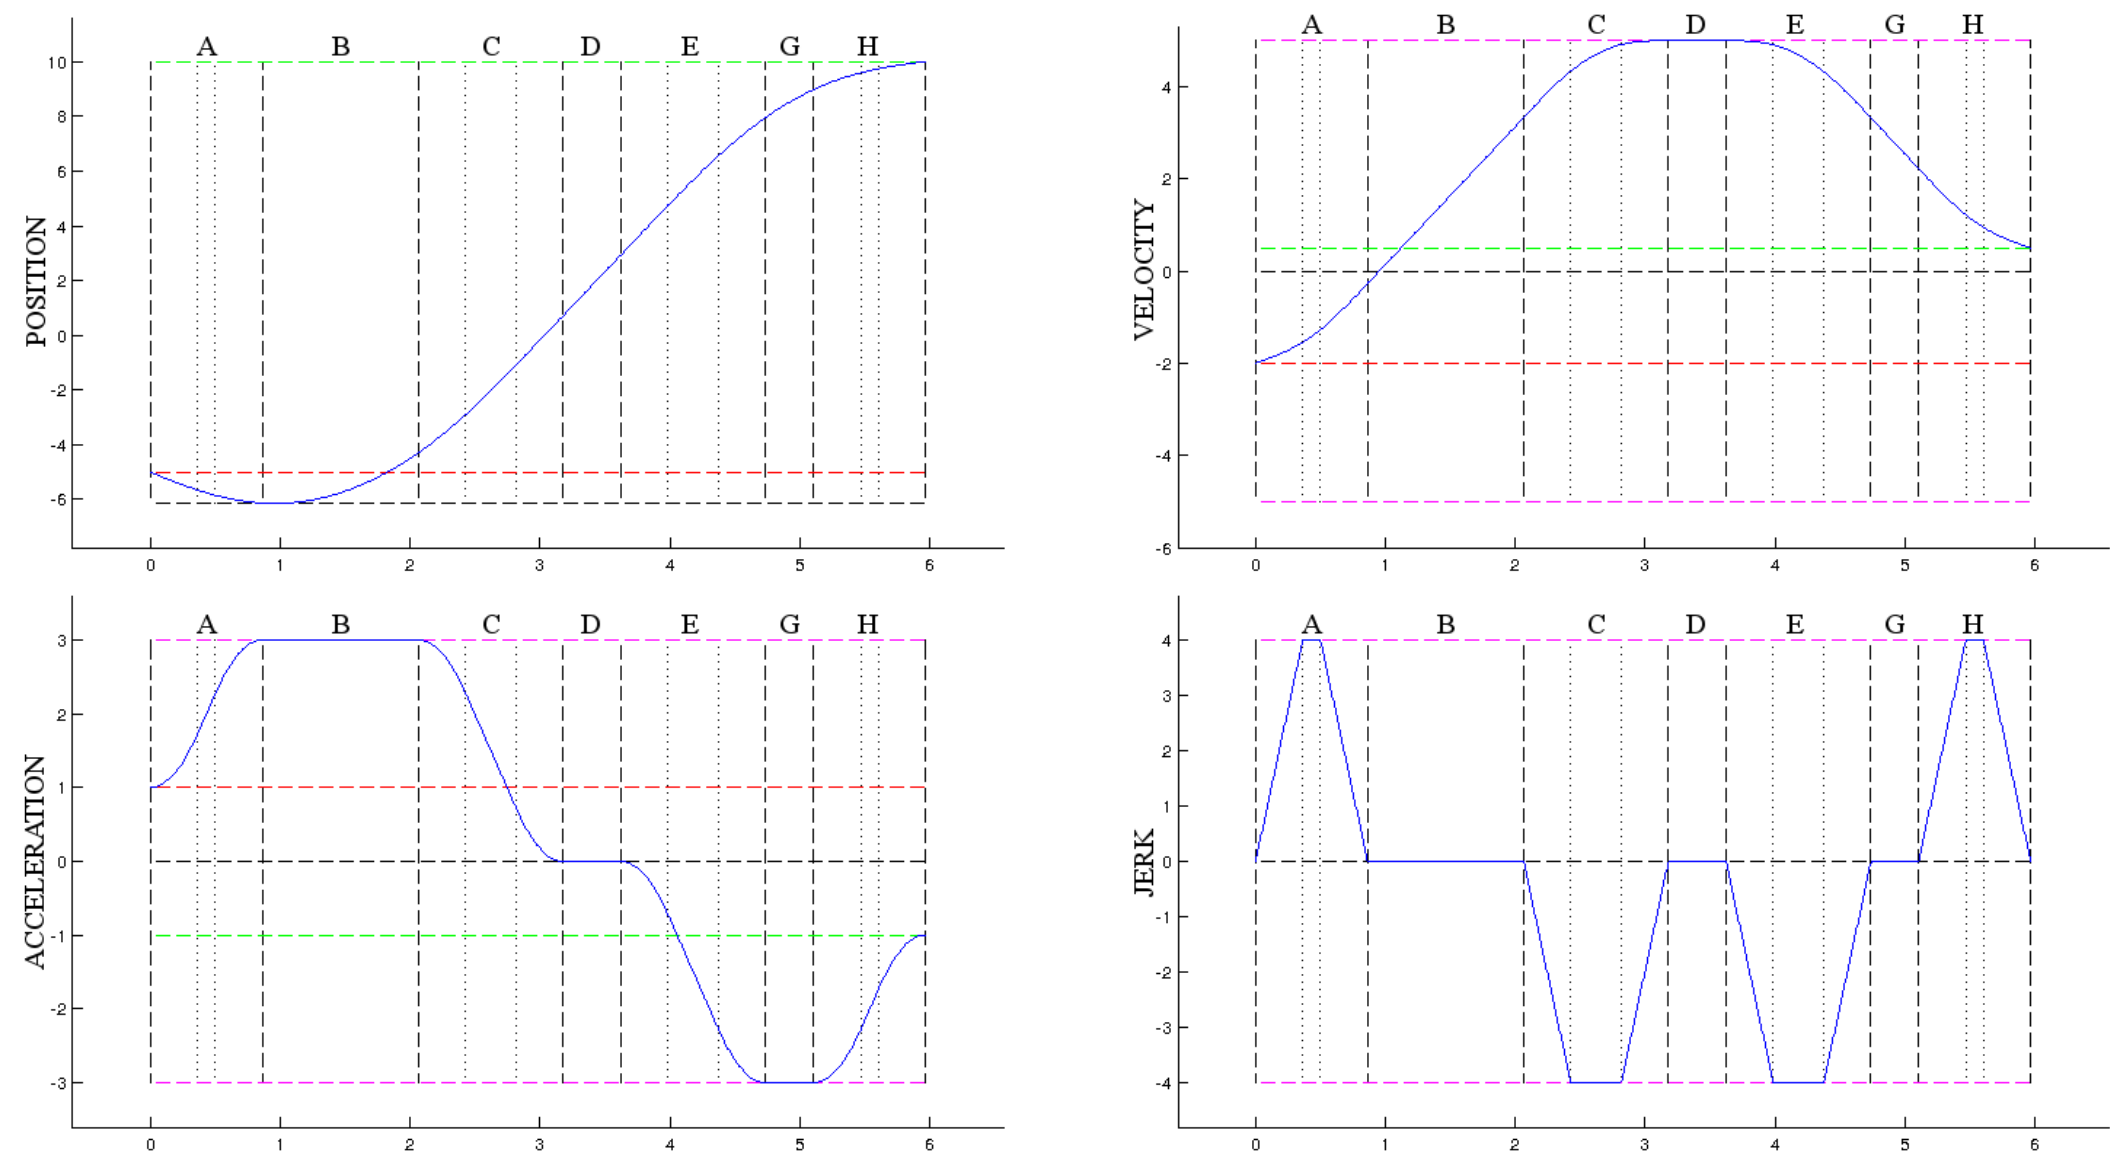
\includegraphics[width=0.99\linewidth]{figures/models/kino.png} 
  \caption{Example of a trajectory generated by the local planner for a single coordinate. The pink dashed lines indicate the bounds for each derivative, while the red and green dashed lines represent the initial and final values, respectively. 
  The letters A, B, C, D, E, G, and H represent the different phases that need to be minimized or maximized during the trajectory planning process.(extracted from~\cite{cKino})}%
  \label{fig:kino}%
\end{figure}

\subsection{Differential drive robot}\label{sec:unic_model}

\subsubsection{Dynamic model}

\begin{figure} [t]
  \centering
  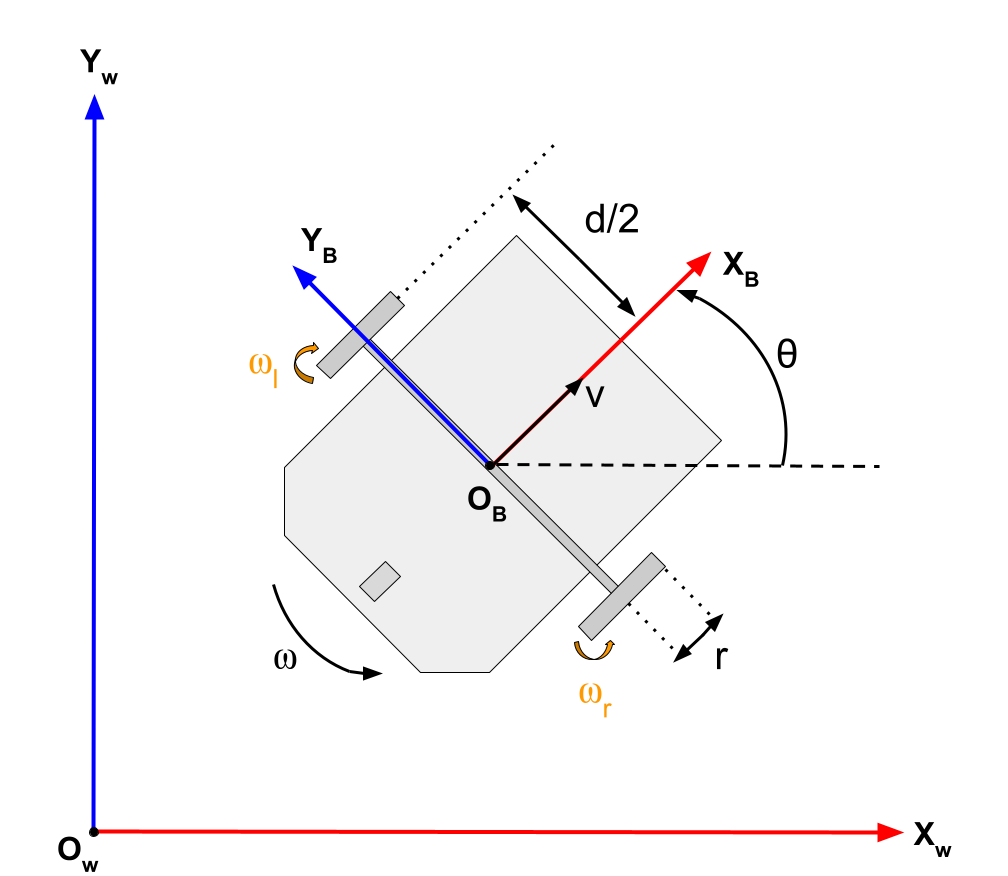
\includegraphics[width=0.6\linewidth]{figures/models/unicycle.png} 
  \caption{Illustration of the main quantities characterizing the differential drive robot.}%
  \label{fig:unicycle}%
\end{figure}

Let the world frame be defined as $F_W \allowbreak = \allowbreak \{O_W, \allowbreak X_W, \allowbreak Y_W\}$ and $F_B = \allowbreak\{O_B, \allowbreak X_B, \allowbreak Y_B\}$ be the differential drive robot body frame attached to its geometric center ($O_B$).
The robot state is defined as $\boldsymbol{q} = [\boldsymbol{x} \, \theta] \in \mathbb{R}^3$ where $\boldsymbol{x} = [x, \, y] \in \mathbb{R}^2$ are the linear positions of $O_B$ in $F_W$ and $\theta$ is the body heading (see Figure~\ref{fig:unicycle}).

Let define the control input vector as $\u = [\omega_r \, \omega_l]^T \in \mathbb{R}^2$, where $(\omega_r, \, \omega_l)$ are respectively the right and left wheel angular velocity.
Let also the robot linear and angular velocities be denoted by $v$ and $\omega$, respectively.
The aforementioned linear and angular velocities are related to the control input vector by mean of an allocation matrix $\boldsymbol{T}$ s.t.:
\begin{equation}\label{eq:unic_alloc}
  \begin{bmatrix}
    v \\
    \omega
  \end{bmatrix}
  =
  \begin{bmatrix}
    \frac{r}{2} & \frac{r}{2}\\
    \frac{r}{2d} & \frac{-r}{2d}
  \end{bmatrix}
  \begin{bmatrix}
    \omega_r \\
    \omega_l
  \end{bmatrix}
  =
  \boldsymbol{T} \u,
\end{equation}
where $d$ is the length between the two wheels, and $r$ is the wheel radius.

The differential drive robot kinematic model can be expressed as:
\begin{equation}\label{eq:unic_dyna}
  \Dot{\q} = 
  \begin{bmatrix}
    cos(\theta) & 0 \\
    sin(\theta) & 0 \\
    0 & 1
  \end{bmatrix} \boldsymbol{T} \u.
\end{equation}
In line with Section~\ref{sec:sensi}, the vector of parameters used in the robot model outlined above that are subject to uncertainty is defined as $\p = [r \, d]^T \in \mathbb{R}^{2}$.

The control task is to let the robot positions $\boldsymbol{x}$ track desired positions $\boldsymbol{x}_d = [x_d, \, y_d] \in \mathbb{R}^2$.
The differential drive robot is an under-actuated system, which is why the heading is excluded from the tracking process; it is induced by the robot dynamic instead.

To perform the tracking task, a \myglsentry{dfl} controller is used (e.g. see~\cite{cDFL}).
This control strategy considers an extended desired trajectory $\q_d(t) = [\boldsymbol{x}_d(t) \, \dot{\boldsymbol{x}}_d(t) \, \ddot{\boldsymbol{x}}_d(t)]^T \in \mathbb{R}^6$, where $\Dot{\boldsymbol{x}}_d(t) \in \mathbb{R}^2$ denote the desired linear velocities, and $\ddot{\boldsymbol{x}}_d(t) \in \mathbb{R}^2$ are the desired linear accelerations.
This trajectory is tracked by mean of the following controller internal states $\boldsymbol{\xi} = [\xi_v \, \xi_x \, \xi_y]^T \in \mathbb{R}^3$, where $\xi_v$ is the dynamic extension of the differential drive robot linear velocity $v$ (see Figure~\ref{fig:unicycle}), and $(\xi_x, \, \xi_y)$ are integral actions. 

By differentiating the robot positions twice, one obtains the following equations for the robot linear accelerations:
\begin{equation*}
  \ddot{\boldsymbol{x}}
  = 
  \begin{bmatrix}
    cos(\theta) & -\xi_v sin(\theta) \\
    sin(\theta) & \xi_v cos(\theta) 
  \end{bmatrix} 
  \begin{bmatrix}
    \dot{v} \\
    \omega
  \end{bmatrix}
  = \boldsymbol{A} \begin{bmatrix}
    \dot{v} \\
    \omega
  \end{bmatrix}
\end{equation*}
This differentiation is essential for formulating the dynamic relationships that enable efficient tracking of the desired positions.

Let the following vectors:
\begin{equation}\label{eq:unic_control_law}
  \left \{
  \begin{array}{l l l}
       \dot{\boldsymbol{x}}_{\xi} = [cos(\theta)\xi_v \, sin(\theta)\xi_v]^T \\
       \boldsymbol{\xi}_{xy} = [\xi_x \, \xi_y]^T \\
       \boldsymbol{\varrho} = \boldsymbol{\ddot{x}}_d + k_v(\boldsymbol{\dot{x}}_d - \dot{\boldsymbol{x}}_{\xi}) + k_p(\boldsymbol{x}_{d} - \boldsymbol{x}) + k_i\boldsymbol{\xi}_{xy}
  \end{array}
  \right .
\end{equation}
where $k_v$, $k_p$ and $k_i$ are the controller gains, s.t. in the following chapters of this thesis, the controller gain vector is defined as $\boldsymbol{k}_c = [k_p, \, k_v \, k_i]^T \in \mathbb{R}^3$.

Without loss of generality, the dynamics of the internal control states can be expressed (refer to~\cite{cDFL} for further details) as follows:
\begin{equation}
  \dot{\boldsymbol{\xi}} = 
  \begin{bmatrix}
    \begin{bmatrix}1 & 0\end{bmatrix}\boldsymbol{A}^{-1}\boldsymbol{\varrho} \\
    \boldsymbol{x}_d - \boldsymbol{x}
  \end{bmatrix}, 
\end{equation}
and the control inputs as:
\begin{equation}
  \u = \boldsymbol{T}_n^{-1} 
  \begin{bmatrix}
    \xi_v \\
    \begin{bmatrix}0 & 1\end{bmatrix}\boldsymbol{A}^{-1}\boldsymbol{\varrho}
  \end{bmatrix},
\end{equation}
where $\boldsymbol{T}_n$ represent the same allocation matrix as in Equation~\ref{eq:unic_dyna} but evaluated on the nominal parameters $\p_n$.

\subsubsection{State interpolation}\label{sec:dubins}

Now that the dynamics of the differential drive robot and its controller are defined, this section presents the local planner used to generate the desired trajectory $\q_d(t) = [\boldsymbol{x}_d(t) \, \dot{\boldsymbol{x}}_d(t) \, \ddot{\boldsymbol{x}}_d(t)]^T \in \mathbb{R}^6$ that is tracked by the \myglsentry{dfl} controller.
The trajectory generation problem is addressed using Dubins curves~\cite{cDubins}. 

This approach ensures smooth and continuous trajectories between two positions $(x^0, y^0)$ and $(x^F, y^F)$ in the x-y plane for systems with constraints on turning radius and forward motion such as the differential drive robot.
The method takes advantage of specified initial and final tangents to the curve (e.g. the differential drive robot heading angle $\theta$, in this case) to create smooth curves that respect the turning constraints.
A Dubins curve is composed of three possible segment types: left turn, right turn, and straight line as depicted in Figure~\ref{fig:dubins}. 
Each segment is designed with an optimal distance, arranged to create the shortest path between the two points $(x^0, y^0)$ and $(x^F, y^F)$. 
This configuration results in one of six possible combinations of segments (e.g., left-straight-right), producing a smooth, continuous path that meets the system turning and heading requirements.

In this thesis, the robot state used to compute such path is defined as $\boldsymbol{\gamma} = [x \, y \, \theta] \in \mathbb{R}^3$.
Once the path is computed, the x and y components are discretized using a specified time step and a constant velocity magnitude denoted $v_{magn}$.
The corresponding velocities along the x- and y-axes are then computed using the finite difference method. 
However, while the resulting velocities are continuous, they are generally not differentiable.
Therefore, in this thesis, the desired accelerations required by Equation~(\ref{eq:unic_control_law}) are set to be zero.
Note that, although the heading is not directly controlled, a desired heading is specified to satisfy the tangent constraints.

\begin{figure} [t]
  \centering
  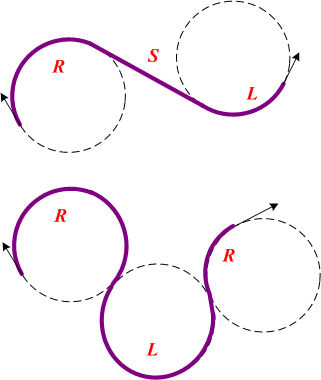
\includegraphics[width=0.4\linewidth]{figures/models/dubins.png} 
  \caption{Illustration of two possible Dubins paths: (top) a right turn, followed by a straight segment, then a left turn; (bottom) a right turn, followed by a left turn, then another right turn. (extracted from~\cite{cFigDubins})}%
  \label{fig:dubins}%
\end{figure}
% \cleardoublepage
% \newpage 
% \ % The empty page
% \newpage
\chapter{Robust and Globally Sensitivity-Optimal Motion Planning}\label{chap:samp}
\markboth{Robust and Globally Sensitivity-Optimal Motion Planning}{}% To set left/right header
% \localtableofcontents

This chapter introduces the first major contribution of this thesis, by leveraging the sensitivity concept discussed in Chapter~\ref{chap:models}.
The contribution of this chapter is twofold:
\begin{enumerate}
    \item Firstly, it addresses the generation of a desired trajectory with minimal sensitivity, ensuring that the closed-loop evolution of $\q(t)$ closely matches its nominal evolution, $\q_n(t)$. 
    While previous work has explored sensitivity optimization for generating locally sensitivity-optimal trajectories \cite{cPi, cTh}, this approach has never been applied within a global sampling-based planning framework that accounts for obstacles. 
    Therefore, the first contribution is to propose methods for efficiently performing global sensitivity-optimal motion planning.
    \item Secondly, this chapter introduces, for the first time, the use of sensitivity-based uncertainty tubes to enforce constraints in both the state and input spaces. 
    This enables the generation of intrinsically-robust motions (i.e. accounting for the controller behavior with respect to uncertainty) that ensures robustness to both the environment and the actuator limits.
\end{enumerate}
This chapter is organized as follows: it first presents in Section~\ref{sec:metrics} how the uncertainty tubes of Section~\ref{sec:tubes} are used to enforce robust constraints in the planning process, as well as the development of an appropriate cost function for performing global sensitivity optimization.
Then, in Section~\ref{sec:unified}, a unified approach is presented, which allows for planning a robust trajectory with optimal sensitivity by directly incorporating the sensitivity computation into the optimal tree-building process (e.g., \myglsentry{rrtstar}). 
This approach is tested on the robot models described in Chapter~\ref{chap:models} showing poor scalability to the system complexity.
Finally, a decoupled approach that shows better efficiency for more complex systems, is introduced in Section~\ref{sec:decoupled}, followed by conclusions in Section~\ref{sec:concl}.

This chapter is associated to the following publication in ICRA 2023: Wasiela, S., Giordano, P. R., Cortés, J., and Simeon, T. (2023, May). "A sensitivity-aware motion planner (samp) to generate intrinsically-robust trajectories." In IEEE International Conference on Robotics and Automation (ICRA) (pp. 12707-12713).

\section{Practical Considerations}\label{sec:metrics}

This section first presents how the uncertainty tubes from Section~\ref{sec:tubes} are used to perform robust feasibility checks, followed by the selection of an appropriate cost function for global sampling-based optimization.

\subsubsection{Robust feasibility check}\label{sec:robust_CC}

As previously mentioned in Chapter~\ref{chap:related_work}, sampling-based algorithms generate global trajectories by combining multiple continuous local trajectories.
During the process, each of these local trajectories are subject to collision checks to determine their feasibility.
However, in this thesis, the collision check is extended to include a more general feasibility test, which also accounts for the control input space. 
This extension ensures that the generated trajectories are not only free from obstacles but also prevent control inputs from reaching saturation. 
Additionally, it accounts for uncertainty in both the state and control input spaces, further enhancing the robustness of the trajectories.
The following section describes how these extended feasibility checks are performed to ensure the robustness of each local trajectory in this context.
It is important to note that these tests are not continuous; rather, they are performed along a discrete representation of the local trajectories.

\paragraph{Robust collision checking}
In this thesis, collision detection is performed using the widely used C implementation of PyBullet~\cite{cBullet}, which operates as follows: 
\begin{enumerate}
    \item It starts with a broad-phase collision detection using \myglsentry{AABBs} to quickly eliminate pairs of objects that are too far apart to collide, allowing the more computationally intensive collision checks to focus only on pairs that are potentially close to each other.
    \item Then, it performs a narrow-phase collision detection that, after potential collision pairs are identified, checks for each pair. For each identified potential collision pair, this phase uses a more precise robot representation (as defined by the user) and specialized collision algorithms to detect actual intersections and determine contact points, normals, and penetration depths.
\end{enumerate}

Extending this procedure to account for robot state uncertainty aims to verify that the resulting extended bounding volume, which the robot may occupy due to the uncertainty, is clear of obstacles.
In this thesis, such bounding volume is computed by considering only the uncertainty in the linear position subspace for simplicity (i.e., the $x,y,z$ subspace for the quadrotor applications or the $x,y$ subspace for the differential drive robot applications).
Several strategies are evaluated based on their computational efficiency, conservatism, and library capabilities:
\begin{enumerate}
    \item The simplest method to account for position uncertainty in collision checking is to compare the distance between the current robot AABB and the nearest obstacle, incorporating the maximum possible deviations by using the worst-case uncertainty tube radius from Equation~\ref{eq:radius} (see~\ref{chap:appendixA} for proof).
    This check corresponds to a uniform scaling of the AABB by the maximum uncertainty radius as depicted in Figure~\ref{fig:CC1}. 
    Since the C PyBullet library does not support re-scaling an existing collision shape on the fly, a new shape must be created whenever scaling is required. 
    By using this straightforward distance check, one can avoid the need to create new shapes.
    However, this method represent a conservative approach as all directions are scaled in the same way.
    \item As mentioned above, a less conservative approach involves creating an extended AABB by scaling the current robot AABB in all directions according to their respective uncertainty radii as shown in Figure~\ref{fig:CC2}. 
    However, this method requires the creation of a new collision shape for each collision test.
    \item The approaches mentioned above, though efficient, are conservative because they only use the current robot AABB and do not leverage narrow-phase collision checks that consider the precise robot mesh representation. 
    However, generating the accurate extended collision shape that incorporates uncertainty, required for the second phase, is challenging, as the library supports only standard primitives like boxes, spheres, cylinders, etc.
    To address this, the third approach approximates the extended collision shape by sampling on the surface of the uncertainty ellipsoid bounding box defined by the uncertainty tube radii, rather than creating a new collision shape (see Figure~\ref{fig:CC3}). 
    While this method more accurately approximates the true extended collision shape than the two first approaches, it requires multiple calls to the collision-checking function for each robot state tested.
\end{enumerate}

\begin{figure}[t]
    \centering
    % Row 1
    \begin{subfigure}{0.4\textwidth}
        \centering
        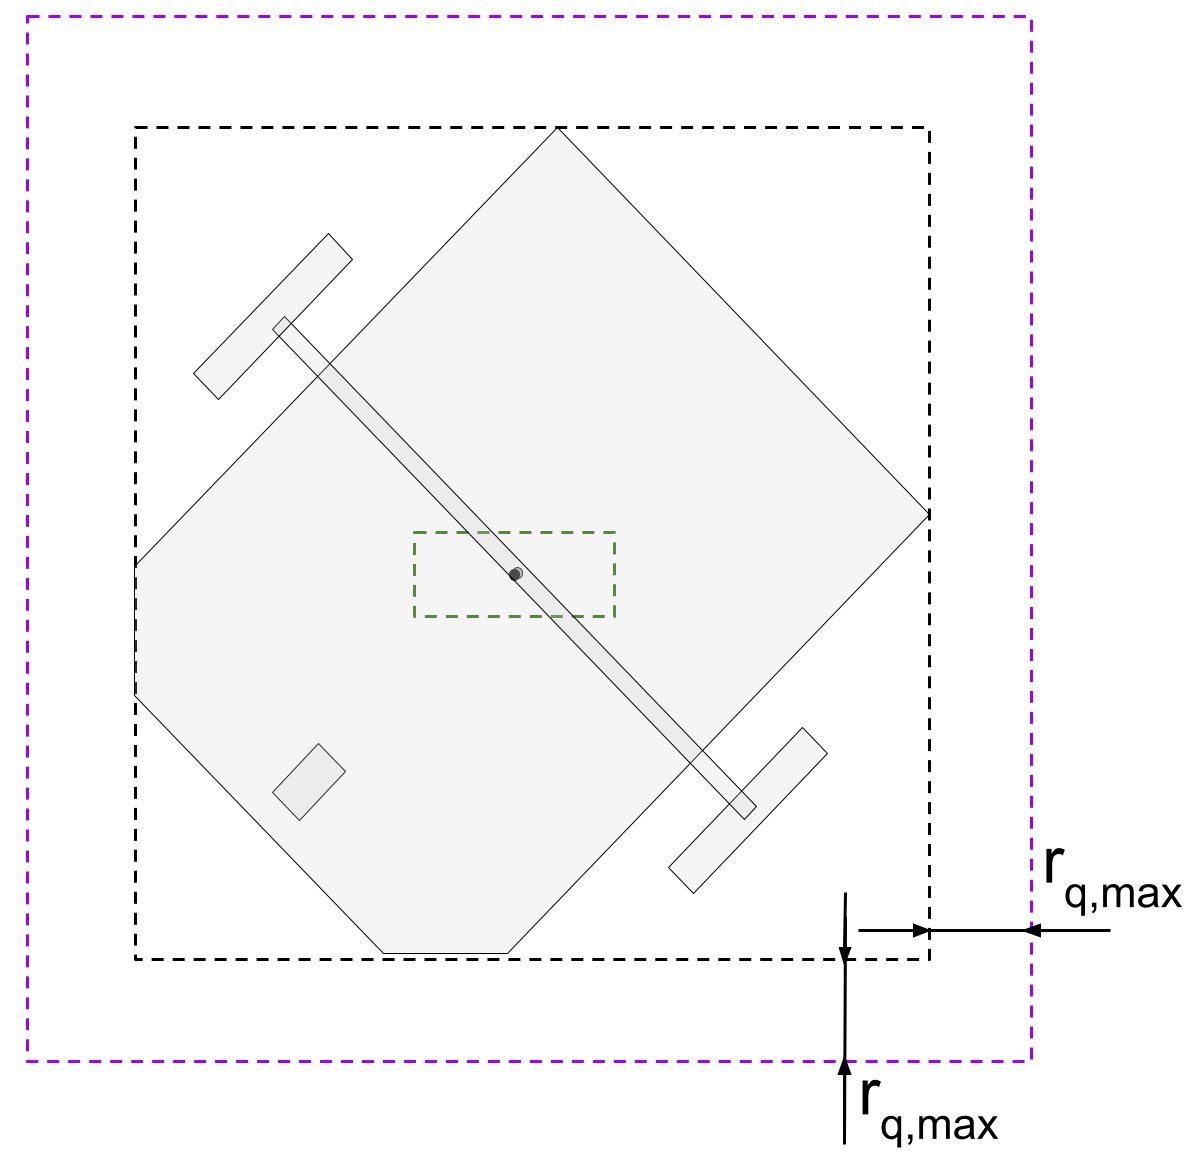
\includegraphics[width=\linewidth]{figures/samp/CC1.png}
        \caption{}
        \label{fig:CC1}
    \end{subfigure}
    % \hfill
    \begin{subfigure}{0.4\textwidth}
        \centering
        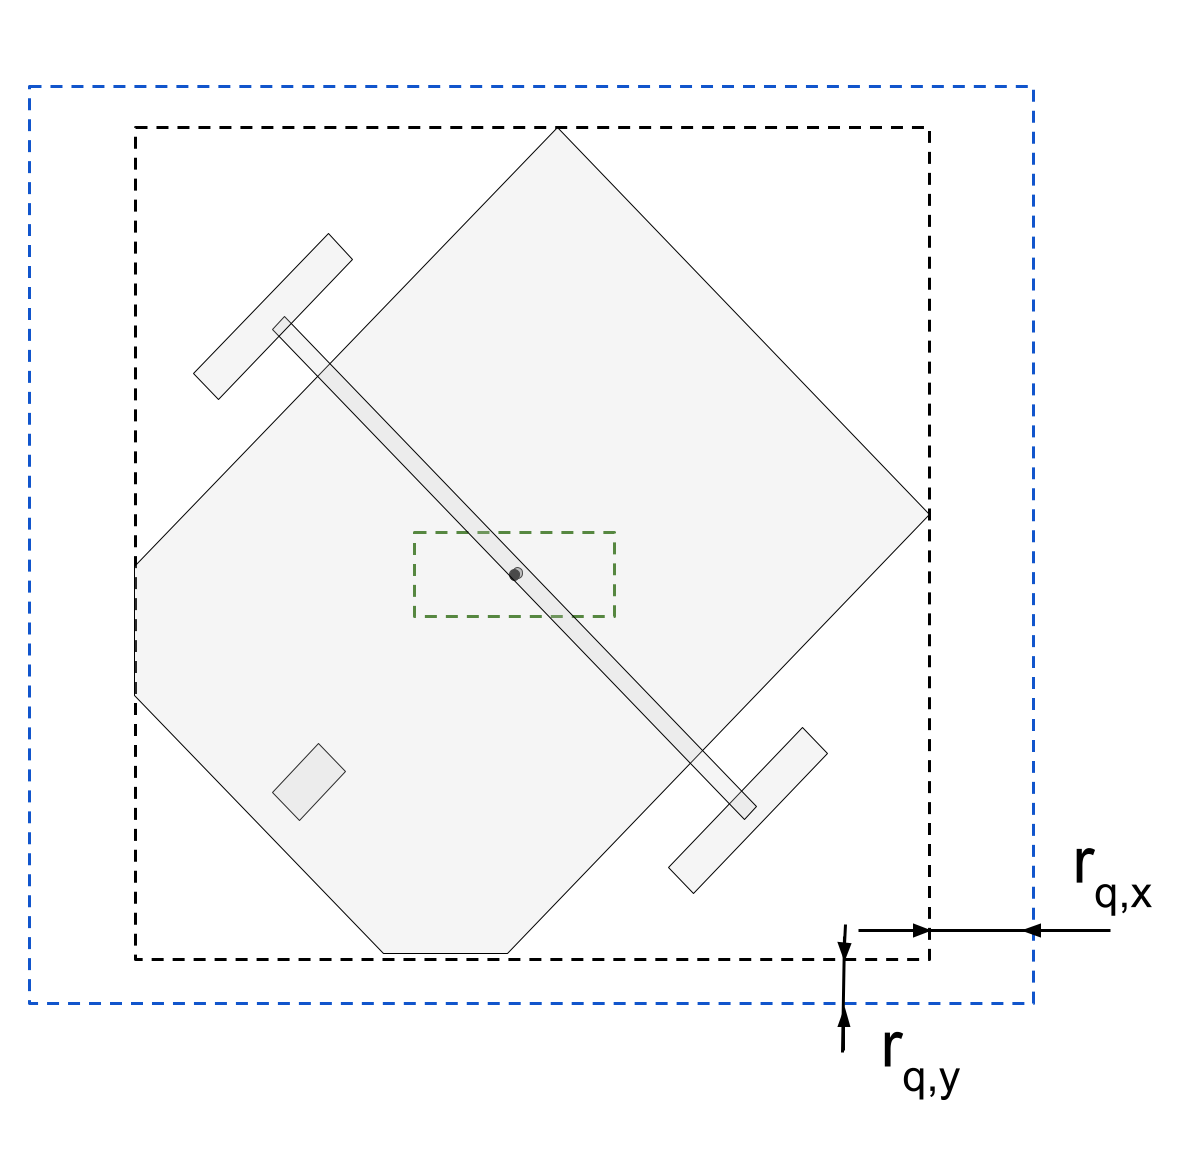
\includegraphics[width=\linewidth]{figures/samp/CC2.png}
        \caption{}
        \label{fig:CC2}
    \end{subfigure}
    
    % Row 2
    \begin{subfigure}{0.4\textwidth}
        \centering
        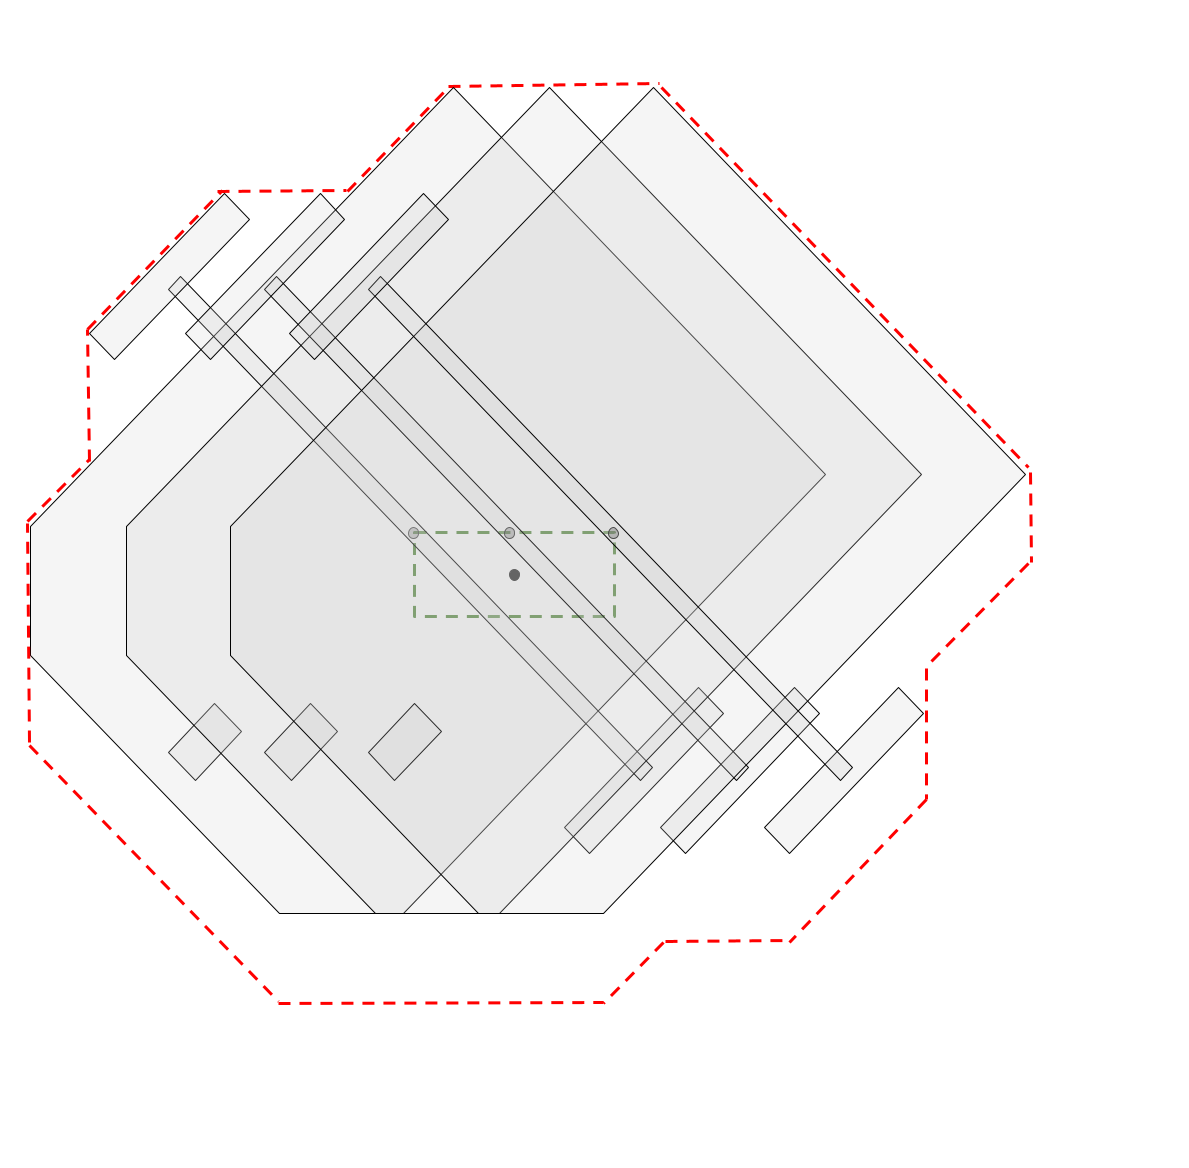
\includegraphics[width=\linewidth]{figures/samp/CC3.png}
        \caption{}
        \vspace{-0.3cm}
        \label{fig:CC3}
    \end{subfigure}
    % \hfill
    \begin{subfigure}{0.4\textwidth}
        \centering
        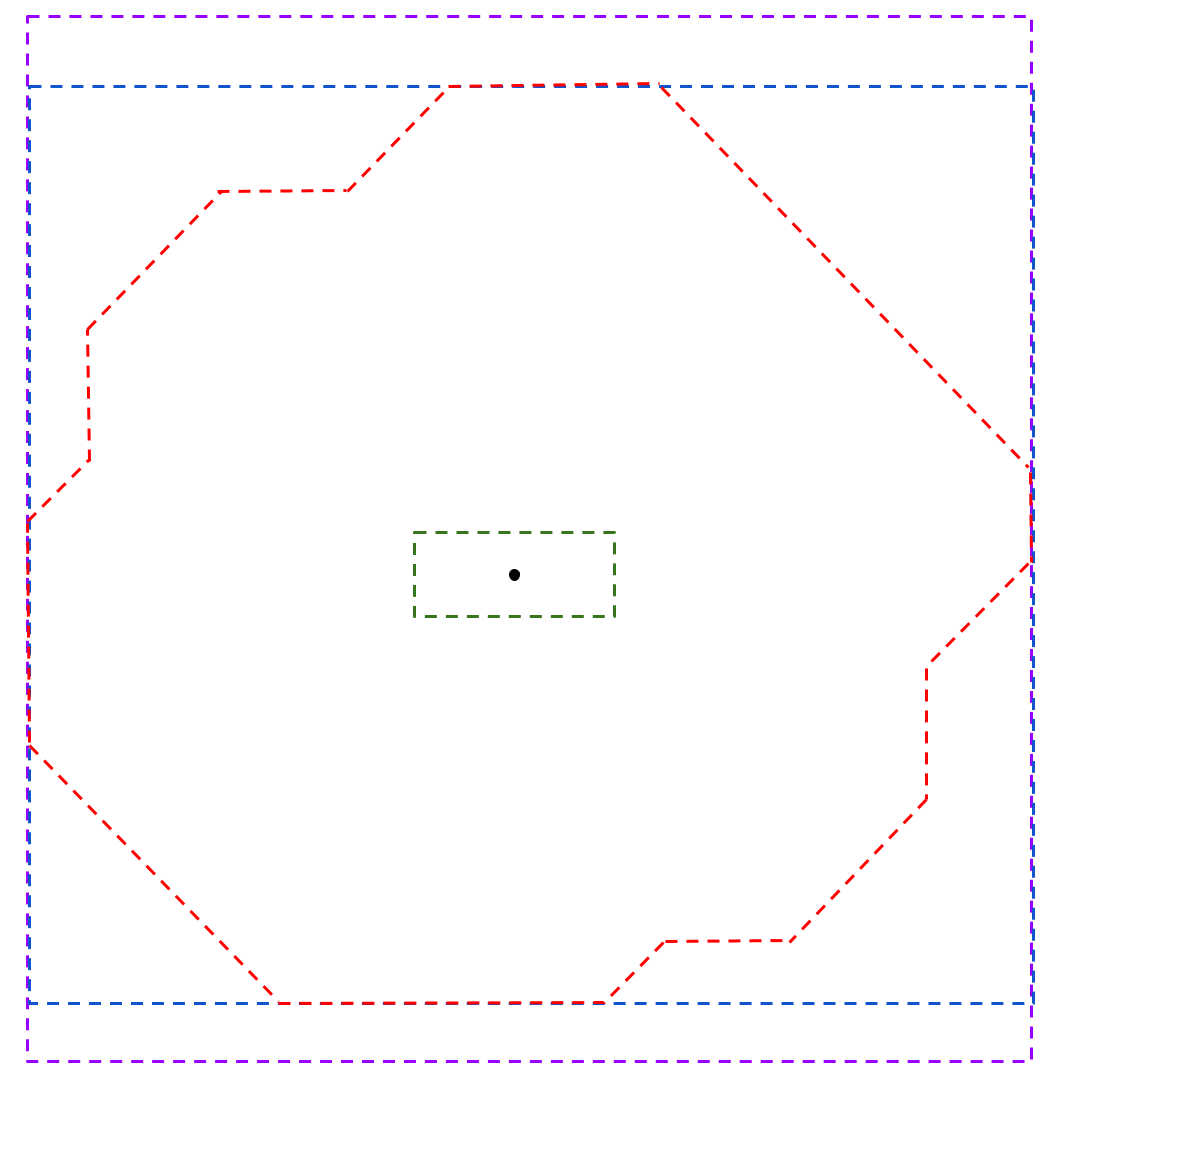
\includegraphics[width=\linewidth]{figures/samp/CCall.png}
        \caption{}
        \vspace{-0.3cm}
        \label{fig:CCall}
    \end{subfigure}

    \caption{Figure showing the space covered by each of the three methods: (a) uniformly scaled AABB, (b) extended AABB, and (c) sampling-based approximation of the extended collision shape, for a differential drive robot with its associated uncertainty ellipsoid bounding box (green) based on computed uncertainty radii. Comparison of the three methods is shown in (d).}
    \label{fig:CCmethods}
\end{figure}

These different approaches enable progressively more precise collision testing, from the first to the third method, as illustrated in the Figure~\ref{fig:CCall} that shows a comparison of the resulting tested collision shapes according to the aforementioned methods for the 2D differential drive robot.
However, this increased accuracy comes at the cost of longer computational times, as noted earlier. 
To quantify this, the mean running time of each method was evaluated based on 1.000 robust collision tests performed using the quadrotor model described in Section~\ref{sec:quad_model}. 
The results indicate that the first method, which involves a simple distance check, has an average runtime of 3 microseconds. 
The second method, which creates an extended uncertain AABB, takes 7 microseconds to compute. 
Finally, the method that approximates the true extended collision shape requires 45 microseconds. 
It is worth mentioning that this last approach involves 14 samples (each corner and the center of each face), and therefore, its runtime can be approximated as linear with respect to the number of samples, compared to a simple test.

Finally, in this thesis, the second approach is used for robust collision checking, as it offers a more precise approximation of the extended collision shape with only a minor increase in computation time than the first approach. 
However, the third approach is employed in the scenario presented in Section~\ref{sec:AOptim}, as it demands a higher level of collision accuracy.
Although the methods employed in this thesis for robust collision checking rely on the uncertainty ellipsoid bounding box computed using Equation~\ref{eq:radius}, the tubes are represented by ellipsoids in the various figures of this manuscript for smoother visualization.

\paragraph{Robust saturation checking}
Then, in this manuscript, the feasibility check is not restricted to the aforementioned collision test, but it also verifies that the robot control inputs does not saturate.
This test is performed by checking that the tube associated with each control input remains in its feasibility domain.
An example of infeasible input for the quadrotor case is presented in Figure.\ref{fig:invalid_inputs},  where the tube (green) around the nominal control input of the first actuator (blue) exceeds the maximum allowed input (red).
Note that this simple test is less costly than the robust collision checking one, it is therefore performed first by mean of computational efficiency. 

\begin{figure} [t]
    \centering
    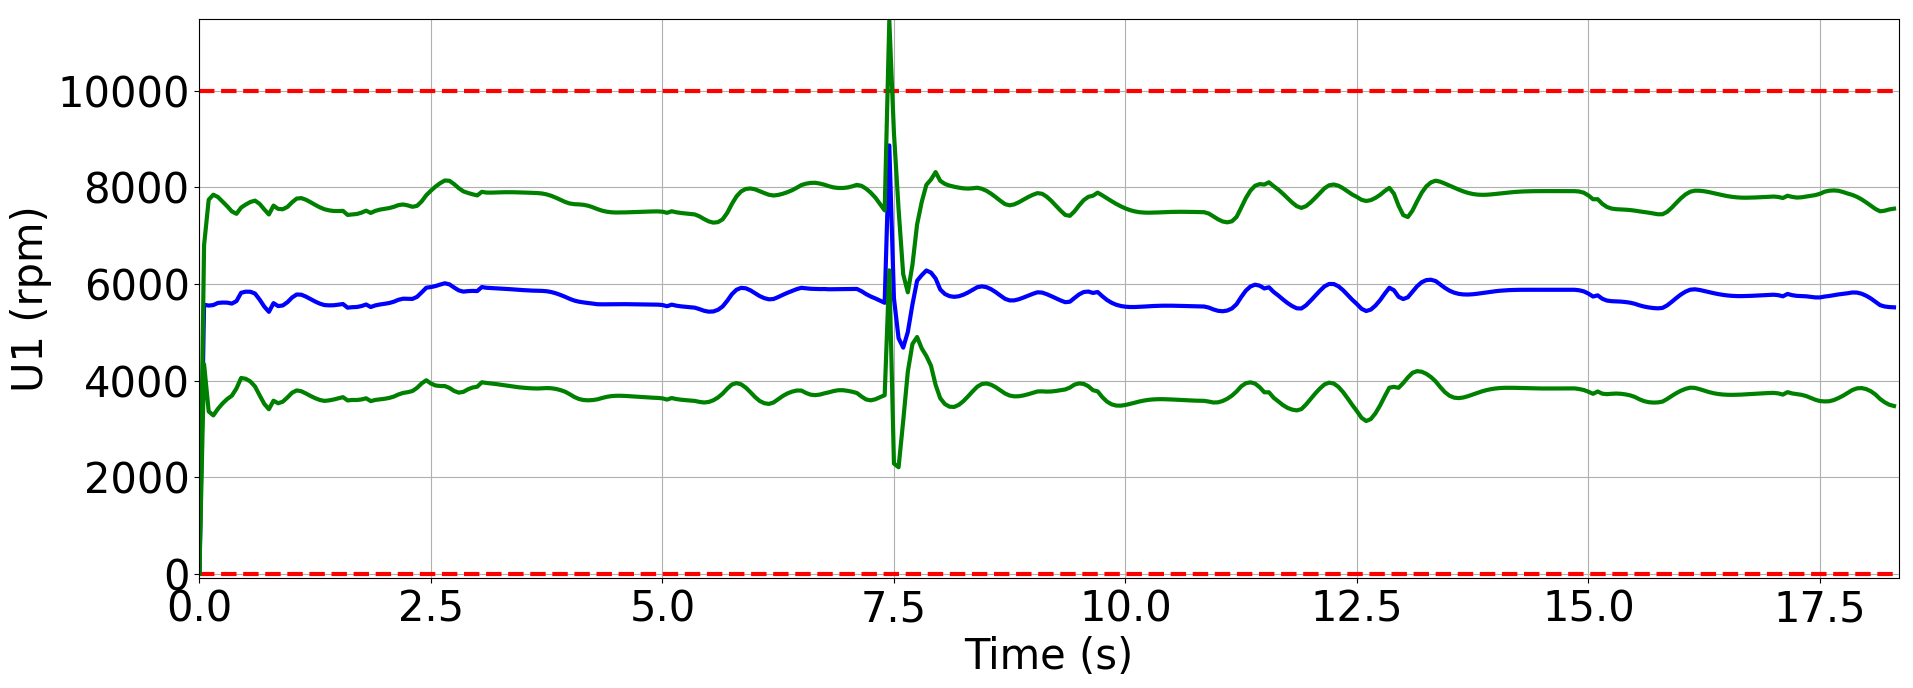
\includegraphics[width=0.8\linewidth]{figures/samp/Invalid_Inputs.png} 
    \caption{Non-robust nominal control input profile for the first rotor of a quadrotor (blue) along a specified trajectory, depicted with its uncertainty tube (green) and the control input limits (red).}%
    \label{fig:invalid_inputs}%
\end{figure}

\subsubsection{Cost function}\label{sec:sensi_cost}

First of all, generating a sensitivity-optimal trajectory requires identifying an appropriate sensitivity-based cost function.
The approaches in~\cite{cPi, cTh} proposed leveraging the Frobenius norm of the sensitivity matrices (Equation~\ref{eq:sensi}).
However, this formulation does not exploit the available information on the uncertainty ranges, $\delta \p$.

Therefore, in this work we consider the largest eigenvalue of the kernel matrix $\bPi(t) \W \bPi(t)^T$ as \emph{sensitivity norm}, since this will represent the largest (worst-case) deviation in the state space. 
In particular, letting $\lambda_i(t)$ be the eigenvalues of $\bPi(t) \W \bPi(t)^T$, we performed a smooth approximation of the $\max(\cdot)$ operator with the $p$-norm:
\begin{equation}
    \lambda_{max}(t)\approx \left(\sum \lambda_{i}(t)^p\right)^{1/p}.
\end{equation} 

However, such function is neither additive (i.e., considering two desired trajectories ($\q_{d,1}(t), \q_{d,2}(t)$), the cost of their concatenation $c(\q_{d,1}(t)|\q_{d,2}(t)) \neq c(\q_{d,1}(t)) + c(\q_{d,2}(t))$), nor monotonic as depicted in Figure~\ref{fig:monotonic}.
Therefore, it is unsuitable for global optimization using sampling-based motion planners like \cite{cRRTstar, cSST}, since they require additive and monotonic objective functions.
The total cost function $c(\q_d(t))$ for a desired trajectory $\q_d(t)$ is then defined as
\begin{equation} \label{eq:cost_function}
    c(\q_d(t))=\int_{t_{0}}^{t_{f}}\lambda_{max}(\tau)d\tau.
\end{equation}
Minimization of this cost will minimize the largest deviation of the state tube along the whole motion.

\begin{figure} [t]
    \centering
    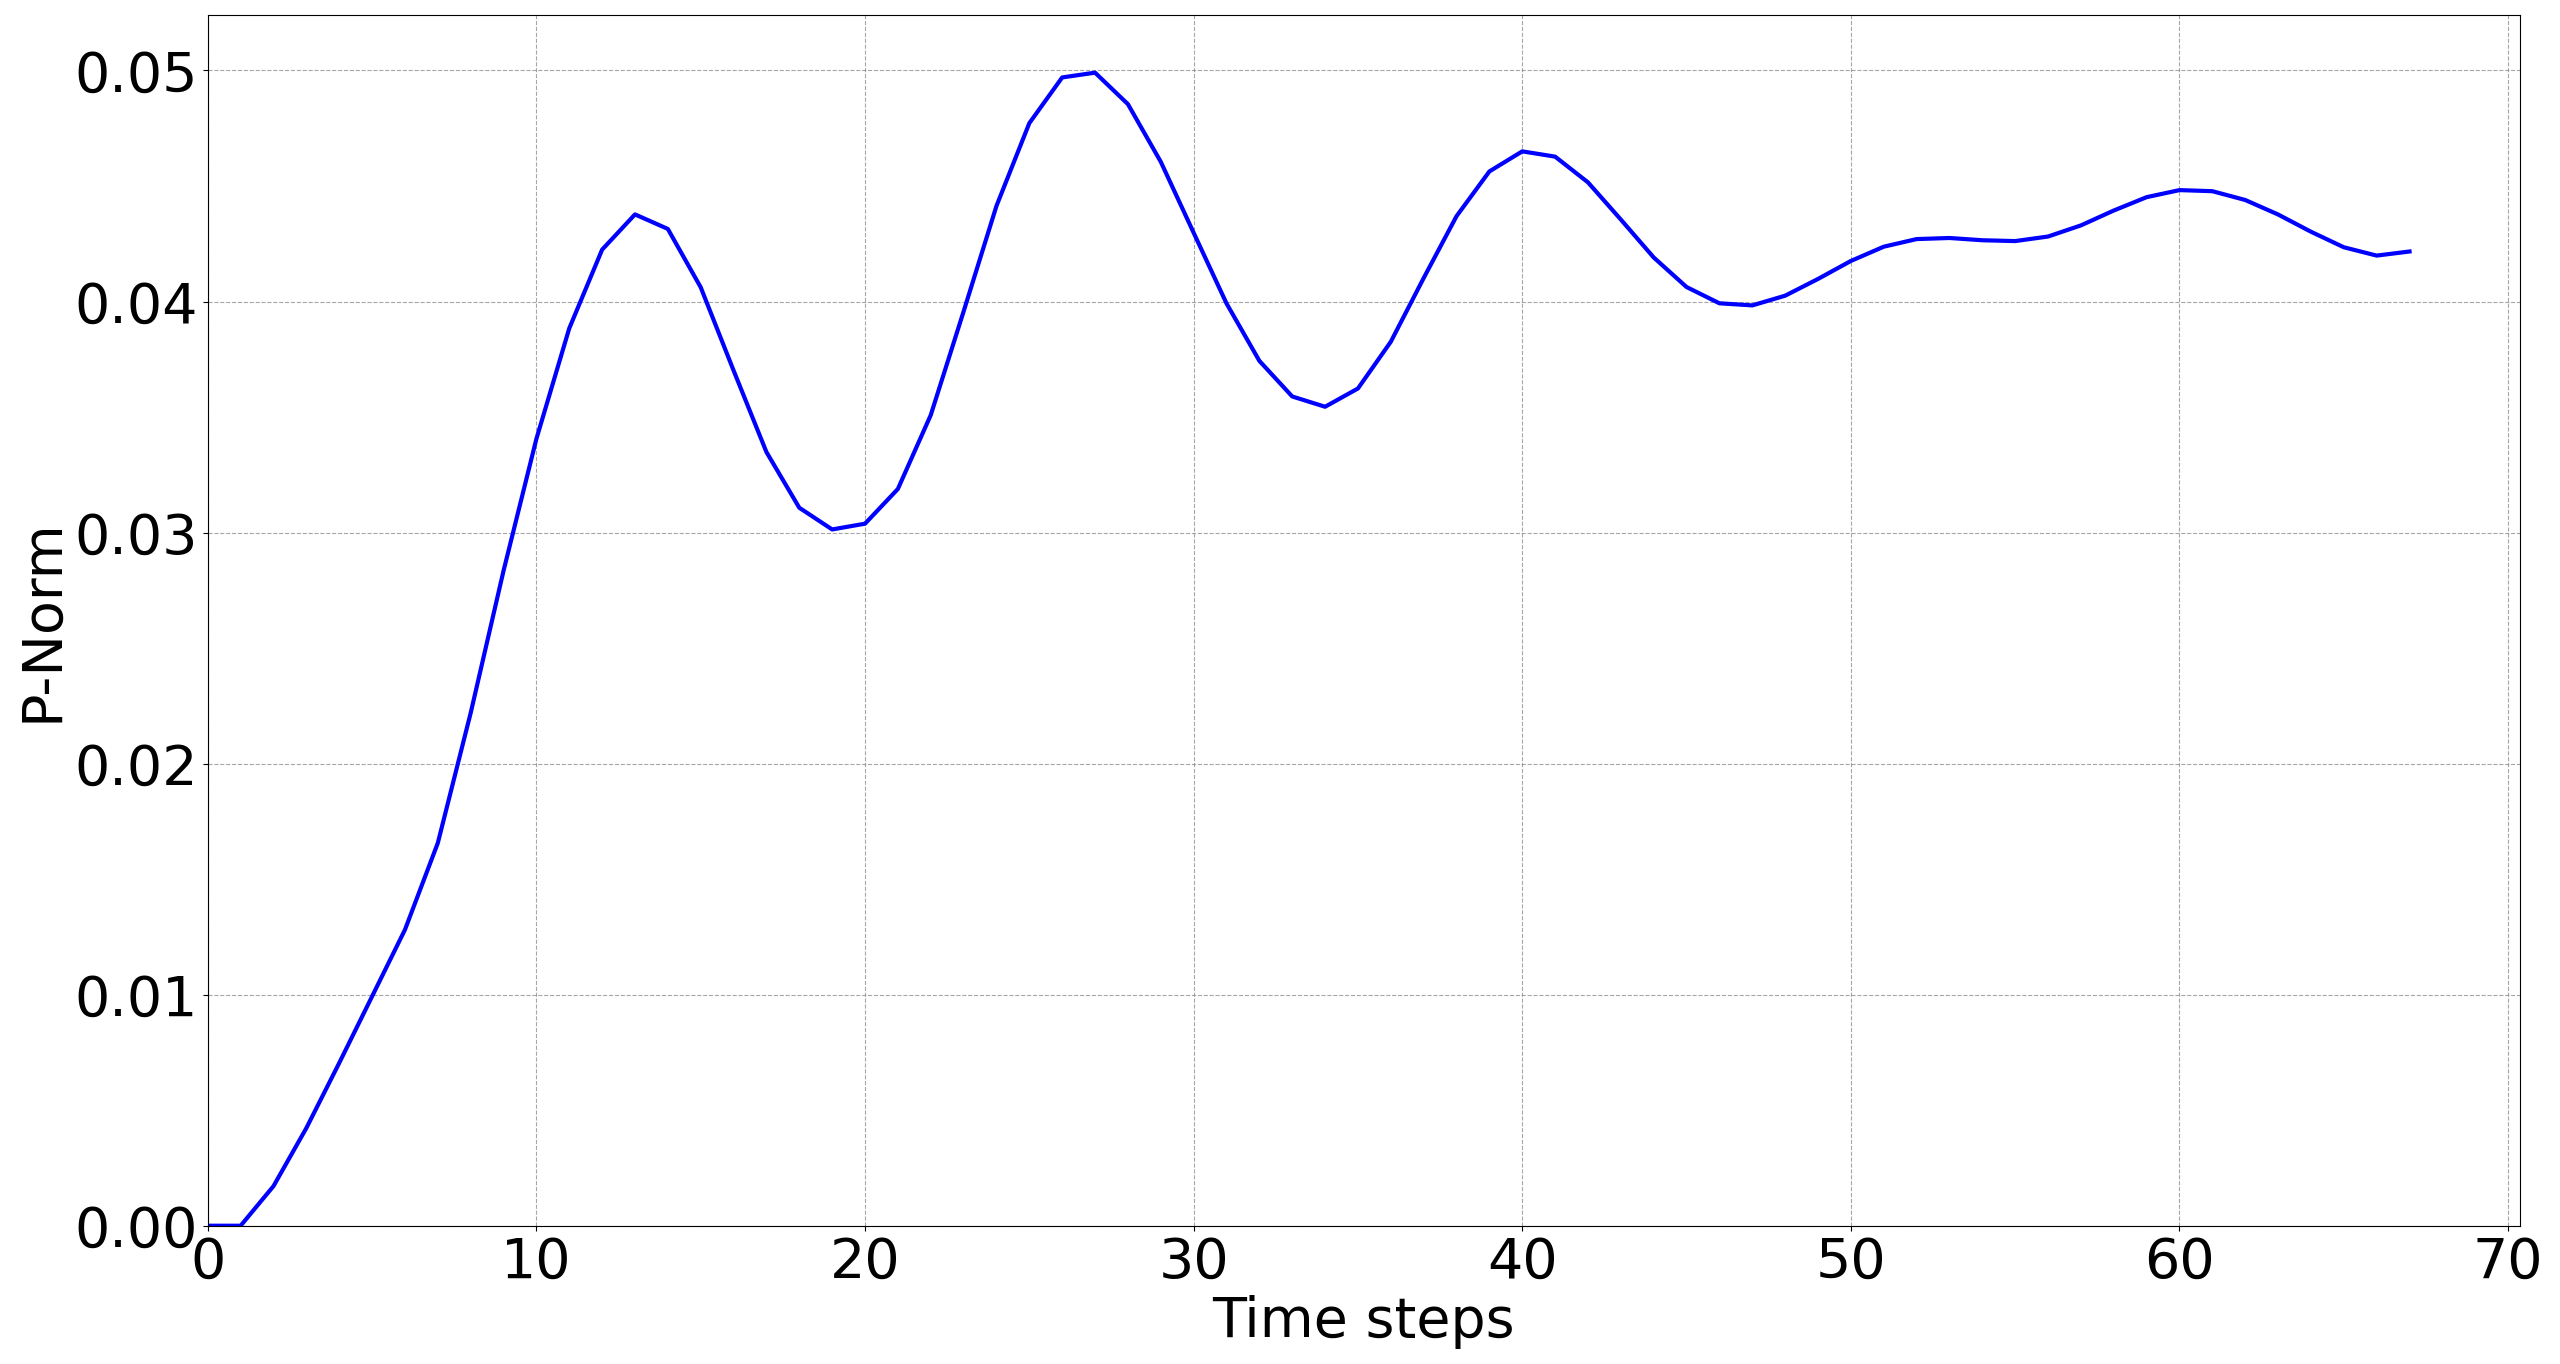
\includegraphics[width=0.7\linewidth]{figures/samp/non_monotoic.png} 
    \caption{Non monotonic p-norm profile along a 70-state trajectory for a quadrotor example.}%
    \label{fig:monotonic}%
\end{figure}

\section{Unified approach}\label{sec:unified}

This section present how the sensitivity matrices and resulting uncertainty tubes computation can be incorporated into any assymptotically-optimal tree planner in order to generate robust and sensitivity-optimal trajectories.  

\subsection{General method}\label{sec:general_method}

As shown in Section~\ref{sec:sensi_and_tubes}, the state/input sensitivity matrices (and resulting uncertainty tubes) are computed by forward integrating the set of \myglsentry{odes} presented by Equation~(\ref{eq:dyna}), Equation~(\ref{eq:ctrl}), and Equation~(\ref{eq:dyna_sensi}).
This computation is performed using the controller time step along a given desired trajectory.
In a sampling-based framework, this computation must be performed at each new extension to assess the trajectory cost and the associated uncertainty tubes for the robust feasibility check.
Although the \myglsentry{odes} need to be solved at each controller time step, it is important to note that the robust feasibility check presented in Section~\ref{sec:robust_CC} can be conducted using a coarser time step.

Furthermore, in a sampling-based context, solving the \myglsentry{odes} from a set of non-zero initial conditions (e.g. $\bPi_0$, $\q^0$ etc.), denoted $S_0$, is required when an extension is made from a node that is not the root.
Therefore, after a feasible extension is made and the new node is added to the structure, the set of final conditions (e.g. $\bPi_F$, $\q^F$,  etc.), denoted $S_F$, must be embedded within the new node.
These conditions are then reused as initial conditions for future extensions.
Moreover, it is important to note that the initial conditions of a given node are determined by the trajectory from the root node. 
As a result, these initial conditions are specific to the parent node, making them applicable only in tree-based planners, where each node has exactly one parent.
Additionally, note that, since dynamics are taken into account, the algorithms presented in this thesis utilize directed data structures (i.e., structures like directed trees that represent dependencies and directionality in motion).

The following section describes how the concepts outlined above can be incorporated into different tree planners to develop robust, sensitivity-aware variants, generally referred to as \gls{samp}.
Note that although the following sections of this chapter focus on asymptotically-optimal planner variants to generate globally sensitivity-optimal trajectories, the same principles can easily be applied to non-asymptotically optimal planners (see Chapter~\ref{chap:sampNN}), such as the standard \gls{rrt}.
 
\subsection{Sensitivity-Aware Motion Planner (SAMP)}\label{sec:samp}

For clarity in the pseudo-code, the temporal notation is omitted in this section. 
Thus, bold symbols refer to time-dependent vectors (e.g., $\q_d$ represents a desired trajectory, $\Rq$ stands for the uncertainty tube radii along a trajectory, etc.), while non-bold symbols represent instantaneous vectors (e.g., $q^{rand}$ denotes a random state without temporal dependencies, and $S_0$ represents the initial conditions of the \myglsentry{odes} at a given state vector, etc.).

\subsubsection{Sensitivity-Aware RRT* (SARRT*)}

\begin{algorithm}[t]
    \caption{SARRT$^* [q^{init}, q^{goal}]$}\label{alg:SARRT*}
    \begin{algorithmic}[1]
        \State $T \gets$ InitTree$({q^{init}, q^{goal}});$
        \While{\textbf{not} StopCondition$(T, {q^{goal}})$}  
            \State $q^{rand} \gets $Sample()$;$
            \State $q^{nearest} \gets$ Nearest$(T,{q^{rand}});$
            \State $\q_d \gets$ LocalPlan$({q^{nearest}},{q^{rand}});$
            \State $S_0 \gets $GetNodeConditions$({q^{nearest}});$
            \State $\left \{\q_n, \u_n, \Rq, \Ru, S_F \right \}  \gets $SolveODEs$(\q_d, S_0);$
            \If {IsRobust$(\Rq,\Ru, \q_n, \u_n)$}
                \State $q^{min} \gets q^{nearest};$
                \State SetNodeConditions$({q^{rand}}, S_{F});$
                \State $Q^{near} \gets$ NearestNodes$(T,{q^{rand}});$
                \State RobustOptimalConnection$(T, Q^{near}, q^{rand}, q^{min});$
                \State RobustRewire$(T, Q^{near}, q^{min});$
            \EndIf
        \EndWhile
        \State \textbf{return} GetTrajectory$(T, q^{init}, q^{goal})$;
    \end{algorithmic}
\end{algorithm}

\begin{algorithm}[t]
    \caption{RobustOptimalConnection$[T, Q^{near}, q^{rand}, q^{min}]$}\label{alg:RobustOptimalConnect}
    \begin{algorithmic}[1]
        \State $c^{min} \gets$ Cost$(q^{rand});$
        \For {each $q^{near} \in Q^{near}$}
            \State $\q_d \gets$ LocalPlan$(q^{near},q^{rand});$
            \State $S_0 \gets $GetNodeConditions$({q^{near}});$
            \State $\left \{\q_n, \u_n, \Rq, \Ru, S_F \right \}  \gets $SolveODEs$(\q_d, S_0);$
            \If {IsRobust$(\Rq,\Ru, \q_n, \u_n)$}
                \If {Cost$(q^{near}) + J(\q_d) < c^{min}$}
                    \State $q^{min} \gets q^{near}; c^{min} \gets$ Cost$(q^{near}) + J(\q_d);$
                    \State SetNodeConditions$({q^{rand}}, S_{F});$
                \EndIf
            \EndIf
        \EndFor
        \State AddNewNode$(T, {q^{rand}});$
        \State AddNewEdge$(T, {q^{min}}, {q^{rand}});$
    \end{algorithmic}
\end{algorithm}

\begin{algorithm}[t]
    \caption{RobustRewire$[T, Q^{near}, q^{min}]$}\label{alg:RobustRewire}
    \begin{algorithmic}[1]
        \For {each $q^{near} \in Q^{near} \backslash \{q^{min}\}$}
            \State $\q_d \gets$ LocalPlan$(q^{rand}, q^{near});$
            \State $S_0 \gets $GetNodeConditions$({q^{rand}});$
            \State $\left \{\q_n, \u_n, \Rq, \Ru, S_F \right \}  \gets $SolveODEs$(\q_d, S_0);$
            \If {IsRobust$(\Rq,\Ru, \q_n, \u_n)$}
                \If {Cost$(q^{rand}) + J(\q_d) <$ Cost$(q^{near})$}
                    \State $q^{parent} \gets$ GetParent$(q^{near});$
                    \State RemoveEdge$(T, q^{parent}, q^{near});$
                    \State AddNewEdge$(T, q^{rand}, q^{near});$
                    \State SetNodeConditions$(q^{near}, S_{F});$
                    \State UpdateChildren$(T, q^{near});$
                \EndIf
            \EndIf
        \EndFor
    \end{algorithmic}
\end{algorithm}

The first implementation presented in Algorithm~\ref{alg:SARRT*} is a variant of the widely used \gls{rrtstar}~\cite{cRRTstar}, denoted \gls{sarrt*} as a particular instance of \myglsentry{samp}.
The tree is initialized with the desired initial and goal robot states, $(q^{init}, q^{goal})$ (line 1), and the algorithm continues until a user-defined stopping criterion is met (line 2).
Such a criterion can include a maximum number of iterations, a maximum runtime, a cost convergence threshold, etc.

The first stage of the algorithm follows the same standard procedure as the vanilla \myglsentry{rrtstar}, including sampling a desired robot state $q^{rand}$ and finding its nearest neighbor $q^{nearest}$ in the tree structure (lines 3 and 4, respectively) using an efficient distance metric.
Then, a local planner (such as the ones presented in Section~\ref{sec:kinosplines} and Section~\ref{sec:dubins}) is employed to generate a desired local trajectory $\q_d$ that connects $q^{rand}$ to $q^{nearest}$.
Next, as discussed in Section~\ref{sec:general_method}, the set of \myglsentry{odes} is solved (line 7) to compute the nominal trajectory $\q_n$, the nominal control inputs $\u_n$, and the uncertainty tubes $(\Rq, \Ru)$, utilizing the initial conditions $S_0$ (line 6).
A robust feasibility check is then conducted along the nominal trajectory and control inputs (line 8), following the procedure outlined in Section~\ref{sec:robust_CC}.
Remember that this test is carried out along the nominal values, as the uncertainty tubes are valid around them, as detailed in Section~\ref{sec:tubes}.
If the extension is feasible, the new node parent is temporarily set to $q^{nearest}$, and the final conditions $S_F$ are temporarily stored within $q^{rand}$ (line 9-10).

Next, to identify the optimal parent of $q^{rand}$, which is temporarily assigned to $q^{min}$, an additional search is conducted within a specified neighborhood $Q^{near}$ (line 11).
Such procedure, depicted in Algorithm~\ref{alg:RobustOptimalConnect}, starts by computing the cost of the unique trajectory from the root node to $q^{rand}$ (line 1).
Then, the optimal parent $q^{min}$ is set to the node in $Q^{near}$ that allows a robust extension while incurring the minimum cost to get to $q^{rand}$ (line 2-9).
Finally, the new node is inserted in the tree with its optimal parent (line 10-11).

Now that the optimal feasible extension is added to the tree, the \myglsentry{sarrt*} checks if any optimal rewiring can be performed using Algorithm~\ref{alg:RobustRewire}.
This rewiring phase checks, for each neighbor $q^{near}$ within $Q^{near}$, whether the trajectory from the root to $q^{near}$, passing through the newly added node $q^{rand}$, can be improved (lines 1-6).
In such case, the parent of $q^{near}$ is updated accordingly, and the final \myglsentry{odes} conditions $S_F$ are also modified (lines 7-10).
Finally, in contrast to the standard \myglsentry{rrtstar}, each child of the newly rewired node must be rechecked for robust feasibility, as their uncertainty tubes and control inputs may have changed due to the updated trajectory resulting from the rewiring (line 11).
Note that this final operation requires re-solving the \myglsentry{odes} for each child node.

\subsubsection{Sensitivity-Aware SST* (SASST*)}

It is important to note that a single iteration of \myglsentry{sarrt*} requires solving the set of \myglsentry{odes} multiple times which leads to a prohibitive computation time per iteration as shown in Section~\ref{sec:samp_simu}.
To mitigate this impact, this section proposes a robust sensitivity-aware variant of the \gls{sst*}~\cite{cSST}, denoted \gls{sasst*} as a particular instance of \myglsentry{samp}. 

The \myglsentry{sst*} algorithm has two key features: it reduces the number of collision checks to just one per iteration and uses Monte Carlo propagation to sample the control input space and perform forward dynamic propagation, eliminating the need for a local planner.
However, since this thesis uses the system closed-loop dynamics for sensitivity computation rather than open-loop Monte Carlo propagation, the latter is replaced by a local planner.

The \myglsentry{sasst*} variant, detailed in Algorithm~\ref{alg:SASST*}, operates as follows:
\begin{itemize}
    \item It first performs metrics and tree initialization (line 1-4) by splitting it into two subsets: $V_{active}$ and $V_{inactive}.$
    Nodes in $V_{active}$ are those with the optimal trajectory cost from the root within their local neighborhoods. 
    In contrast, nodes in $V_{inactive}$ while suboptimal in trajectory cost, are preserved in the tree to maintain connectivity, as they have children with better trajectory costs in their respective neighborhoods. 
    \item To define local neighborhoods, the algorithm leverages an auxiliary set of states called "witnesses," denoted as $W$ (line 5). 
    Each witness $w \in W$ is associated with a single representative node in the tree, stored in the $w.rep$ field of the witness (line 6).
    This representative node corresponds to the trajectory with the lowest cost from the root within a distance $\delta_s$ of the witness $w$.
    Any nodes within the $\delta_s$-neighborhood of $w$ that have a higher trajectory cost than $w.rep$ are removed from the active set $V_{active}$.
    \item Then, until a user defined criterion is met, the algorithm performs for N iterations:
    \begin{enumerate}
        \item A best-first selection that samples a random state from the state space and finds the best node in terms of cost from the root within a distance of $\delta_{BN}$ in the active set of the tree. 
        This node, referred as $q^{selected}$, represents the state to be propagated (line 9).
        \item Then, instead of the original Monte Carlo propagation, a random state $q^{rand}$ is sampled within a maximum distance of $q^{selected}$ (line 10), analogous to sampling a control input and propagation duration in the vanilla algorithm.
        The local trajectory connecting the two state is computed (line 11) and, as discussed in Section~\ref{sec:general_method}, the set of \myglsentry{odes} is solved (line 12-13) before performing the robust feasibility check (line 14) presented in Section~\ref{sec:robust_CC}.
        \item If the local trajectory is robustly feasible, the set $W$ is used by the IsNodeLocallyTheBestSST procedure (line 15) to check whether the newly sampled state $q^{rand}$ dominates the $\delta_s$-neighborhood of its closest witness and to update the witness set $W$ accordingly.
        \item Then, the sample is added to the tree (line 16-17), and the sets of active and inactive nodes are updated.
        Nodes that no longer belong to any of these sets are pruned (line 18).
    \end{enumerate}
    \item Finally, after the N iterations, if the stopping criterion is not met, the hyperparameters of the algorithm are updated (line 19-21).
    These parameters are responsible for the algorithm asymptotic optimality and convergence. 
    The algorithm gradually reduces the radii $\delta_s$ and $\delta_{BN}$, enabling it to explore new homotopic classes over time.
\end{itemize}

Note that in this implementation the \myglsentry{odes} need to be solved only once per iteration compared to the \myglsentry{sarrt*} implementation.

\begin{algorithm}[t]
    \caption{SASST$^* [q^{init}, q^{goal}, N_0, \delta_{BN,0}, \delta_{s,0}, \xi]$}\label{alg:SASST*}
    \begin{algorithmic}[1]
        \State $j \gets 0; N \gets N_0;$
        \State $\delta_{s} \gets \delta_{s,0}; \delta_{BN} \gets \delta_{BN,0};$
        \State $V_{active} \gets \{q^{init}, q^{goal}\}, V_{inactive} \gets \emptyset;$
        \State $T \gets$ InitTree$(V_{active}, V_{inactive});$
        \State $w_0 \gets q^{init}, w_G \gets q^{goal}, W \gets \{w_0, w_G\};$
        \State $w_0.rep \gets q^{init}, w_G.rep \gets q^{goal};$
        \While{\textbf{not} StopCondition$(T, {q^{goal}})$}  
            \For{N iterations}
                \State $\{q^{selected}, q^{rand}\} \gets $BestFirstSelectionSST$(V_{active}, \delta_{BN});$
                \State $q^{rand} \gets$ Sample$(q^{selected}, d_{max});$
                \State $\q_d \gets$ LocalPlan$({q^{selected}},{q^{rand}});$
                \State $S_0 \gets $GetNodeConditions$({q^{selected}});$
                \State $\left \{\q_n, \u_n, \Rq, \Ru, S_F \right \}  \gets $SolveODEs$(\q_d, S_0);$
                \If {IsRobust$(\Rq,\Ru, \q_n, \u_n)$}
                    \If{IsNodeLocallyTheBestSST$(q^{rand}, W, \delta_s)$}
                        \State $V_{active} \gets V_{active} \cup \{q^{rand}\};$
                        \State AddNewEdge$(T, q^{selected}, q^{rand});$
                        \State PruneDominatedNodesSST$(q^{rand}, V_{active}, V_{inactive});$
                    \EndIf
                \EndIf
            \EndFor
            \State $\delta_s \gets \xi\delta_s; \delta_{BN}\gets\xi\delta_{BN};$
            \State $j \gets j+1;$
            \State $N \gets (1+$log $j)\xi^{-(d+1)j}N_0;$
        \EndWhile
        \State \textbf{return} GetTrajectory$(T, q^{init}, q^{goal})$;
    \end{algorithmic}
\end{algorithm}

\subsection{Simulation results}\label{sec:samp_simu}

This section presents the results of trajectory planning using the previously discussed variants, evaluated based on computation time, and robustness for the two systems introduced in Chapter~\ref{chap:models}.
To assess the impact of planning robust, globally sensitivity-optimal trajectories, both \myglsentry{sarrt*} and \myglsentry{sasst*} are compared with their respective non-robust vanilla versions, which focus on optimizing trajectory length.
The objective of this section is to quantify the ability of the proposed variants to generate robust solutions, and to evaluate the impact of solving \myglsentry{odes} multiple times within a sampling-based framework.
All implementations are performed using the \gls{ompl}~\cite{cOMPL}.

\subsubsection{Differential drive robot}

\paragraph{Setup}

This section presents results for the differential drive robot model depicted in Section~\ref{sec:unic_model}, with the following set of uncertain parameters $\p = [r, \, d]^T \in \mathbb{R}^{2}$.
The nominal value vector is set to $\p_n = [0.1m, \, 0.4m]^T$, with an associated uncertainty range of $\delta\p = [3\%, \, 3\%]^T$, representing the percentage deviation from their corresponding nominal values.
Therefore, in this differential drive robot application, $\bPi \in \mathbb{R}^{3\times2}$, $\bPixi\in \mathbb{R}^{3\times2}$, and $\bPi \in \mathbb{R}^{2\times2}$.
As a result, the computations necessary to find the uncertainty tubes involve solving 19 \myglsentry{odes}.
The uncertainty tubes considered for this application are defined as $\Rq = [r_x, \, r_y]^T \in \mathbb{R}^2$, representing the uncertainty tubes along the x,y-axes of the state respectively, and $\Ru = [r_{u1}, \, r_{u2}]^T \in \mathbb{R}^2$, representing the uncertainty tubes along the two control input space axes ($\omega_r$ and $\omega_l$).
The controller gains are set to $\k_c = [1.5, \, 8.0, \, 0.2]^T$, and the control inputs limits are set to $\u_{max} = [60, \, 60]^T$, corresponding to the maximum speed of the two wheels expressed in rad.s$^{-1}$.

Remind that the local planning method used is the Dubins path planner (see Section~\ref{sec:dubins}). 
Using the true cost-to-go as the distance metric is known to be computationally inefficient. 
However, as the cost of Equation~(\ref{eq:cost_function}) is strongly correlated to the trajectory length through the integral term, the length of the Dubins curves is used as the distance function heuristic. 
The time step used for the solving the \myglsentry{odes} and to perform the robust feasibility checks is set to 0.05s.
The algorithms stopping criterion is defined by a cost convergence threshold of 5\%.

The hyperparameters for \myglsentry{sasst*} are selected based on the recommendations in~\cite{cSST}, with the following values: $N_0 = 5000$, $\delta_s = 0.5$, $\delta_{BN} = 1$, and $\xi = 0.9$.
For the maximum local distance, $d_{max}$ is set to 1.0.

The standard \myglsentry{rrtstar} does not impose a maximum distance for local connections, which can lead to excessively long trajectories when two sampled states are far apart.
These trajectories frequently fail the robust feasibility check, leading to significant computational effort spent on computing uncertainty tubes only to detect early infeasibility. 
This inefficiency slows down tree growth.

To address this, and following the approach used in the original \myglsentry{ompl} implementation, a maximum distance is introduced for local trajectories. 
This adjustment does not compromise the algorithm properties, as longer trajectories can still be formed by chaining several shorter local trajectories. 
While this approach requires more iterations to ensure adequate space coverage and convergence, it results in more efficient tree growth under robustness constraints, as illustrated in Figure~\ref{fig:unic_tree}.

Consequently, throughout this thesis, a maximum local trajectory length of 1.0 (meters or seconds according to the local planner used) is also applied to the proposed \myglsentry{sarrt*} and \gls{sarrt} (see Chapter~\ref{chap:sampNN}) variants.

\paragraph{Results}

\begin{table*}[t!]
    \centering
    \begin{tabular}{l|llll|}
    \cline{2-5}
        & \multicolumn{1}{c|}{RRT$^{*}$} & \multicolumn{1}{c|}{SARRT$^*$} & \multicolumn{1}{c|}{SST$^*$} & \multicolumn{1}{c|}{SASST$^*$} \\ \hline
    \multicolumn{1}{|c|}{Success (\%)} & \multicolumn{1}{c|}{3.3} & \multicolumn{1}{c|}{\textbf{100.0}}  & \multicolumn{1}{c|}{17.3}  &  \multicolumn{1}{c|}{\textbf{100.0}}   \\ \hline
    \multicolumn{1}{|c|}{Plan time (s)} & \multicolumn{1}{c|}{952 $\pm$ 201}   & \multicolumn{1}{c|}{4145 $\pm$ 639} & \multicolumn{1}{c|}{819 $\pm$ 155}  &   \multicolumn{1}{c|}{2148 $\pm$ 320}  \\ \hline
    \end{tabular}
    \caption{
    \label{tab:samp_unicycle}
    Average planning time and success rate (no crash) of the simulated motions planned by \myglsentry{rrtstar}, \myglsentry{sarrt*}, \myglsentry{sst*}, and \myglsentry{sasst*} over 10 plans and 30 simulations per plan, for the differential drive robot.}
\end{table*}

Results, graph profiling RRT*/RSARRT*, SST*/RSASST*

\begin{figure} [h]
    \centering
    \includesvg[width=0.8\linewidth]{figures/samp/profiling_unic.svg} 
    \caption{Evolution of the sensitivity as a function of the planning time of a \myglsentry{sasst*} (green), and of \myglsentry{sarrt*} (red) for the quadrotor application.}%
    \label{fig:profiling_unic}%
\end{figure}

\begin{figure} [t]
    \centering
    \subfloat[\centering Unbounded local trajectory length]{{\includegraphics[width=0.4\linewidth]{figures/samp/rrtstar_unbounded.png} }}%
    \subfloat[\centering Bounded local trajectory length]{{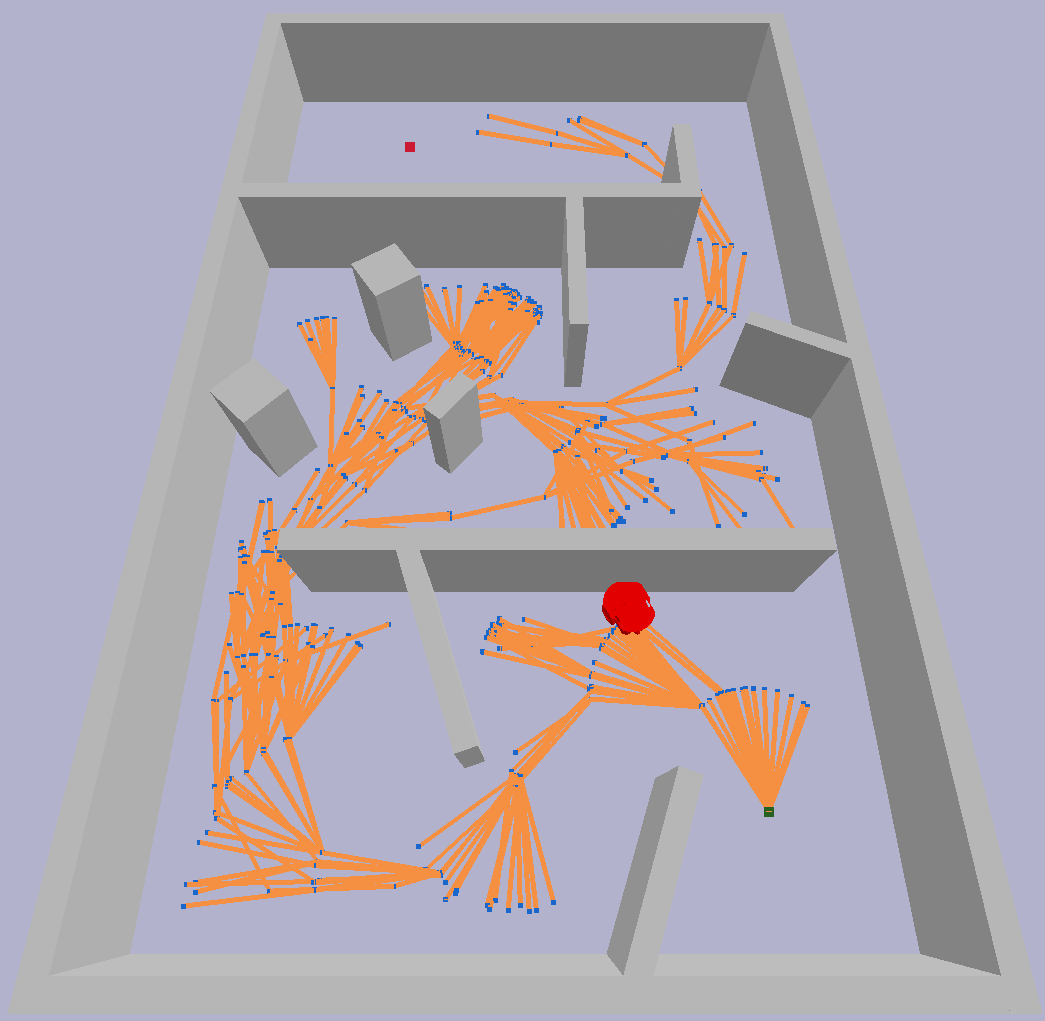
\includegraphics[width=0.4\linewidth]{figures/samp/rrtstar_bounded.png} }}%
    \caption{Tree generated after 1.000 iterations of the \myglsentry{sarrt*} algorithm for the differential drive robot shown for two cases: (a) with unbounded local trajectory length, (b) with bounded local trajectory length.}%
    \label{fig:unic_tree}%
\end{figure}

\subsubsection{Quadrotor robot}

\paragraph{Setup}

\paragraph{Results}

As explained in Section~\ref{sec:unified}

\begin{figure} [t]
    \centering
    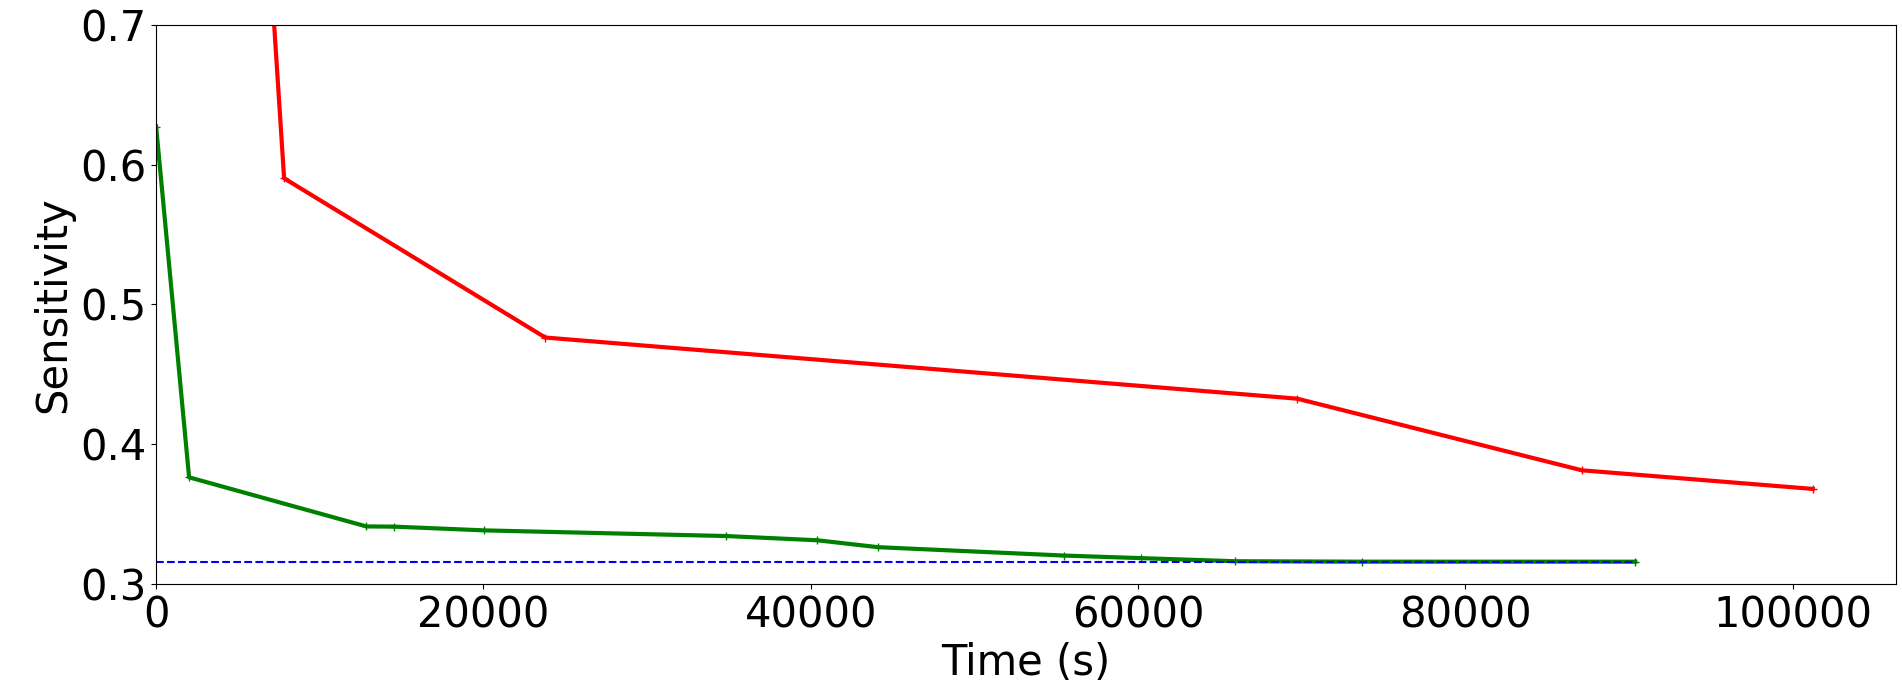
\includegraphics[width=0.7\linewidth]{figures/samp/SSTstar_Sensi.png} 
    \caption{Evolution of the sensitivity as a function of the planning time of a \myglsentry{sasst*} (green), and of \myglsentry{sarrt*} (red) for the quadrotor application.}%
    \label{fig:samp_quad_time}%
\end{figure}

\begin{figure} [h]
    \centering
    \includesvg[width=0.8\linewidth]{figures/samp/profiling_quad.svg} 
    \caption{Evolution of the sensitivity as a function of the planning time of a \myglsentry{sasst*} (green), and of \myglsentry{sarrt*} (red) for the quadrotor application.}%
    \label{fig:profiling_quad}%
\end{figure}

Results, graph profiling RRT*/RSARRT*, SST*/RSASST*

Very long planning time because very large state space to be explored, lots of iteartions needed to provide a good coverage of the space for convergence.
In view of the part taken by the ODEs it's not tracktable, while it is still tracktable for "standard" RRT* optimizing time.

The key bottleneck is the number of time we need to solve the \myglsentry{odes}. 
For more complex system such as quadrotor it is still not tracktable.

\section{Decoupled approach}\label{sec:decoupled}

As demonstrated in Section~\ref{sec:samp_simu}, the proposed \myglsentry{samp} variants are efficient for simple systems but face challenges with more complex ones, such as the quadrotor. 
Achieving effective state-space coverage and convergence to a solution requires thousands of iterations, each involving the resolution of \myglsentry{odes}. 
This creates a bottleneck for the method, particularly when solving the \myglsentry{odes} takes tens of milliseconds, as is common in complex systems.
Therefore, this section introduces a decoupled approach that minimizes the frequency of solving the \myglsentry{odes}, offering a more efficient algorithm for complex systems, such as quadrotor, to generate robust trajectories with near-optimal sensitivity.

\subsection{Algorithms}

Since the cost function of Equation~(\ref{eq:cost_function}) corresponds to the integration of the sensitivity over the trajectory, it is then noticeable that starting from an initial (near) time-optimal trajectory helps to produce initial solutions of rather good quality w.r.t. the sensitivity cost.
The proposed decoupled approach is based on a lazy sensitivity-aware variant, generally referred to as \gls{lazysamp}, that plans a robust (near) time-optimal trajectory.
This trajectory is then locally optimized for minimizing the cost function~(\ref{eq:cost_function}) via a robust variant of the `shortcut' technique classically used to smooth solutions of randomized planners~\cite{cShortcut}. 

\subsubsection{Lazy Sensitivity-Aware RRT* (LazySARRT*)}\label{sec:lazy_rrt*}

\begin{algorithm}[t]
    \caption{LazySARRT$^* [q^{init}, q^{goal}]$}\label{alg:LazySARRT*}
    \begin{algorithmic}[1]
        \State $T \gets$ InitTree$({q^{init}, q^{goal}});$
        \While{\textbf{not} StopCondition$(T, {q^{goal}})$}  
            \State $q^{rand} \gets $Sample()$;$
            \State $q^{nearest} \gets$ Nearest$(T,{q^{rand}});$
            \State Extend$(T, q^{rand}, q^{nearest});$
            \State $Q_{sol} \gets CheckForSolution(T, q^{init}, q^{goal});$
            \If{$Q_{sol} \neq \emptyset$}
                \For { i = 0 and  i < size($Q_{sol}$)-1}
                    \State $S_0 \gets $GetNodeConditions$(Q_{sol}^{i});$
                    \State $\q_d \gets $LocalPlan$(Q_{sol}^{i}, Q_{sol}^{i+1});$
                    \State $\left \{\q_n, \u_n, \Rq, \Ru, S_F \right \}  \gets $SolveODEs$(\q_d, S_0);$
                    \If {\textbf{not} IsRobust$(\Rq,\Ru, \q_n, \u_n)$}
                        \State $T \gets $RobustReconnect$(T, Q_{sol}^{i});$
                        \State break;
                    \EndIf
                \EndFor
            \EndIf
        \EndWhile
        \State \textbf{return} GetTrajectory$(T, q^{init}, q^{goal})$;
    \end{algorithmic}
\end{algorithm}

This section present the \gls{lazysarrt*}, as a particular instance of \myglsentry{lazysamp}, that plans a robust (near) time-optimal trajectory.
The algorithm not only provides a (near) time-optimal trajectory but also ensures that the resulting trajectory is collision-free w.r.t. the state uncertainties and also that control inputs remain in their allowed bounds.
However, as highlighted in Section~\ref{sec:unified}, the number of \myglsentry{odes} computation within the \myglsentry{rrtstar} must remain as limited as possible to avoid a too long computing time. 
For this reason, trajectory robustness is checked in a lazy way, only when a better solution is found, and reconnecting the nodes optimally if necessary.
Consequently, unlike the \myglsentry{samp} methods described in Section~\ref{sec:samp}, the tree built by the lazy variant is not inherently robust; only the final solution meets the robustness requirements.

Algorithm~\ref{alg:LazySARRT*} provides the pseudo-code of the \myglsentry{lazysarrt*} variant.  
The first stage applies the unmodified \myglsentry{rrtstar} (line 1-5) where the Extend procedure performs the standard collision checking (i.e. without uncertainty tubes), optimal connection, and rewiring phase for the given sample  $q^{rand}$ as in~\cite{cRRTstar}.
The algorithm then verifies at each iterations whether a new, lower-cost solution has been discovered. 
If a better solution is identified, the set of nodes $Q_{sol}$, which enables the reconstruction of this solution, is retrieved (line 6).

Next, for each local trajectories between two consecutive nodes in this set, the \myglsentry{odes} are solved, and the uncertainty tubes computed (line 9-11).
The algorithm then verifies the robust feasibility of the local trajectory using the robustness test outlined in Section~\ref{sec:robust_CC}. 
If a local trajectory is found to be non-robustly feasible, all nodes in the tree connected to $Q_{sol}^i$ are disconnected and reconnected using the RobustReconnect procedure (line 13).

The RobustReconnect procedure may differ depending on the specific \myglsentry{lazysamp} variant used (see Chapter~\ref{chap:sampNN}). 
In the case of \myglsentry{lazysarrt*}, where maintaining an optimal tree is required, it operates as follows:
\begin{itemize}
    \item For all tree nodes, a set of robust infeasible parent $Q_{collide}$ is maintained. 
    The RobustReconnect procedure starts by adding $Q_{sol}^i$ in the set of infeasible parents of $Q_{sol}^{i+1}$ (i.e. $Q_{sol}^i$ will no longer be considered as a potential parent for the node $Q_{sol}^{i+1}$).
    \item Then, all the nodes of the tree from $Q_{sol}^i$ are disconnected, and for each of them, the vanilla Extend procedure is executed considering their associated $Q_{collide}$ set.
    As in the standard \myglsentry{rrtstar}, an optimal re-connection phase is first attempted.
    \item If no re-connection is found for a node, then the node is deleted from the tree. 
    Otherwise, the rewiring phase is carried out considering the $Q_{collide}$ set.
\end{itemize}

The output of \myglsentry{lazysarrt*} is a (near) time-optimal trajectory that is feasible in terms of both collision avoidance and actuator saturation, accounting for uncertainties.
It is however not optimized in terms of the sensitivity. 
Therefore, its robustness can be further improved.

\subsubsection{Sensitivity Aware Shortcut}

In order to improve the sensitivity-based cost function, a local optimization is performed using a simple robust sensitivity-aware variant of the 'shortcut' smoothing algorithm~\cite{cShortcut}, called \gls{SAshortcut} and described in Algorithm~\ref{alg:SAshortcut}. 
A more detailed discussion regarding the robust sensitivity-aware local optimization can be found in Chapter~\ref{chap:sampNN}.

The algorithm is first initialized with the robust trajectory resulting from the \myglsentry{lazysarrt*} presented above (line 1).
It is important to note that the robustness of the initial trajectory is a crucial assumption, as the \myglsentry{SAshortcut} algorithm does not guarantee the generation of a robust trajectory if the initial trajectory is not robust.
Nevertheless, the algorithm preserves this robustness throughout its local optimization process.
Then, the algorithm randomly samples two states $\{q_d^{1}, q_d^{2}\}$, along the current best trajectory (line 3).
Next, it computes the local trajectory between the two samples $\q_{d,shct}$ (line 7).
To minimize the frequency of solving the \myglsentry{odes}, a lazy approach is employed.
First, the algorithm ensures that the proposed shortcut is collision-free (line 8). 
Unlike the classical shortcut method, which compares only the costs of the original and proposed trajectory segments, the entire trajectory is reevaluated to incrementally compute the sensitivity cost (lines 9–13).
Finally, if the new solution has a lower sensitivity cost (line 14), then a robust feasibility check is performed before updating the trajectory portion in case of success (line 15).

\begin{algorithm}[t]
    \caption{SAShortcut [$\q_{d,SARRT^*}$]}\label{alg:SAshortcut}
    \begin{algorithmic}[1]
        \State $\{\q_{d,best}, cost_{best}\} \gets \{\q_{d,SARRT^*}, $Cost$(\q_{d,SARRT^*}) \};$
        \State $q_d^{init} \gets \q_{d,best}^0; q_d^{goal} \gets \q_{d,best}^F;$
        \While{\textbf{not} StopCondition$()$} 
            \State $\{q_d^{1}, q_d^{2}\} \gets$ SampleOnTraj$(\q_{d,best});$
            \State $\q_{d,start} \gets $LocalPlan$(q_d^{init}, q_d^{1});$
            \State $\q_{d,end} \gets $LocalPlan$(q_d^{2}, q_d^{goal});$
            \State $\q_{d,shct} \gets $LocalPlan$(q_d^{1}, q_d^{2});$
            \If{CollisionFree$(\q_{d,shct})$}
                \State $\q_{d,new} \gets \q_{d,start}+\q_{d,shct}+\q_{d,end};$
                \State $cost_{new} \gets $Cost$(\q_{d,new});$
                \If{CostBetterThan$(cost_{new}, cost_{best})$}
                    \State $S_0 \gets $GetNodeConditions$(q_d^{init});$
                    \State $\{\q_n, \u_n, \Rq, \Ru, S_F\}  \gets $SolveODEs$(\q_{d,new}, S_0);$
                    \If {\textbf{not} IsRobust$(\Rq,\Ru, \q_n, \u_n)$}
                        \State $\{\q_{d,best}, cost_{best}\} \gets \{\q_{d,new}, cost_{new}\};$
                    \EndIf
                \EndIf
            \EndIf
        \EndWhile
    \State \textbf{return} $\q_{d,best}$
    \end{algorithmic}
\end{algorithm}

\subsection{Simulation results}
\subsubsection{Differential drive robot}
\subsubsection{Quadrotor robot}

\paragraph{Setup}

\paragraph{Results}

\newcolumntype{C}[1]{>{\centering\arraybackslash }b{#1}}
\begin{table*}[t]
    \centering
    \begin{tabular}{|C{0.185\linewidth}||C{0.095\linewidth}|C{0.12\linewidth}|C{0.12\linewidth}|C{0.09\linewidth}|}
     \hline
      & U-shape & 2-Way$_{low}$ & 2-Way$_{high}$ & 3D \\
     \hline
     \hline
     Time \myglsentry{sasst*}  (s) & 7221 & 16615 & 23194 & 26875 \\
     \hline
     Time \myglsentry{lazysarrt*} (s) & \textbf{673} \quad $\pm$ 247& \textbf{2506} \quad\quad $\pm$ 305& \textbf{3271} \quad\quad $\pm$ 440& \textbf{2388} \quad $\pm$ 342\\
     \hline
     Time \myglsentry{SAshortcut} (s) & \textbf{453} \quad $\pm$ 191& \textbf{374} \quad\quad $\pm$ 173& \textbf{753} \quad\quad $\pm$ 104& \textbf{577} \quad $\pm$ 229\\
     \hline 
     Decoupled approach time gain (\%)  & 84.4 & 82.7 & 82.6 & 89.0 \\
     \hline
     \hline
      Cost \myglsentry{sasst*} & 0.317 & 0.292 & 5.127 & 0.510 \\
     \hline
      Cost decoupled approach & \textbf{0.324} \quad $\pm$ 0.003& \textbf{0.298} \quad $\pm$ 0.002& \textbf{5.274} \quad\quad $\pm$ 0.041& \textbf{0.523} \quad $\pm$ 0.071\\
     \hline
      Sub-optimality decoupled approach (\%) & 2.21 & 2.01 & 2.87 & 2.55 \\
     \hline
    \end{tabular}
    \caption{
    \label{tab:lazySAMP_quad}
    Average values of costs and computing times for the different methods in several environments.
    Standard deviations are provided for the SAMP results only as the SST$^*$ results do not contain enough runs.
    }
\end{table*}

The performances of the decoupled approach were evaluated in three different environments, also considering different parametric uncertainties.
For the 2D environments (U-shape and 2-Way) we forced the quadrotor to evolve on a plane by producing kinosplines (see Section~\ref{sec:kinosplines}) only between samples constrained within this plane.
The sensitivity-optimal trajectories used as references to evaluate the proposed decoupled approach were computed using a \myglsentry{sasst*} as described in Section~\ref{sec:samp}.

Table~\ref{tab:lazySAMP_quad} gathers the average computing times of \myglsentry{sasst*} and of the two core procedures of the proposed decoupled approach (\myglsentry{lazysarrt*}, \myglsentry{SAshortcut}), as well as the average final cost found by \myglsentry{sasst*} and \myglsentry{SAshortcut}. 
The mean values associated with \myglsentry{sasst*} were obtained over 3 runs (due to the very high computing time) while those associated with the proposed decoupled approach are averaged over 10 runs.

\paragraph{2D U-Shape Environment} 

\begin{figure}[t]
    \centering
    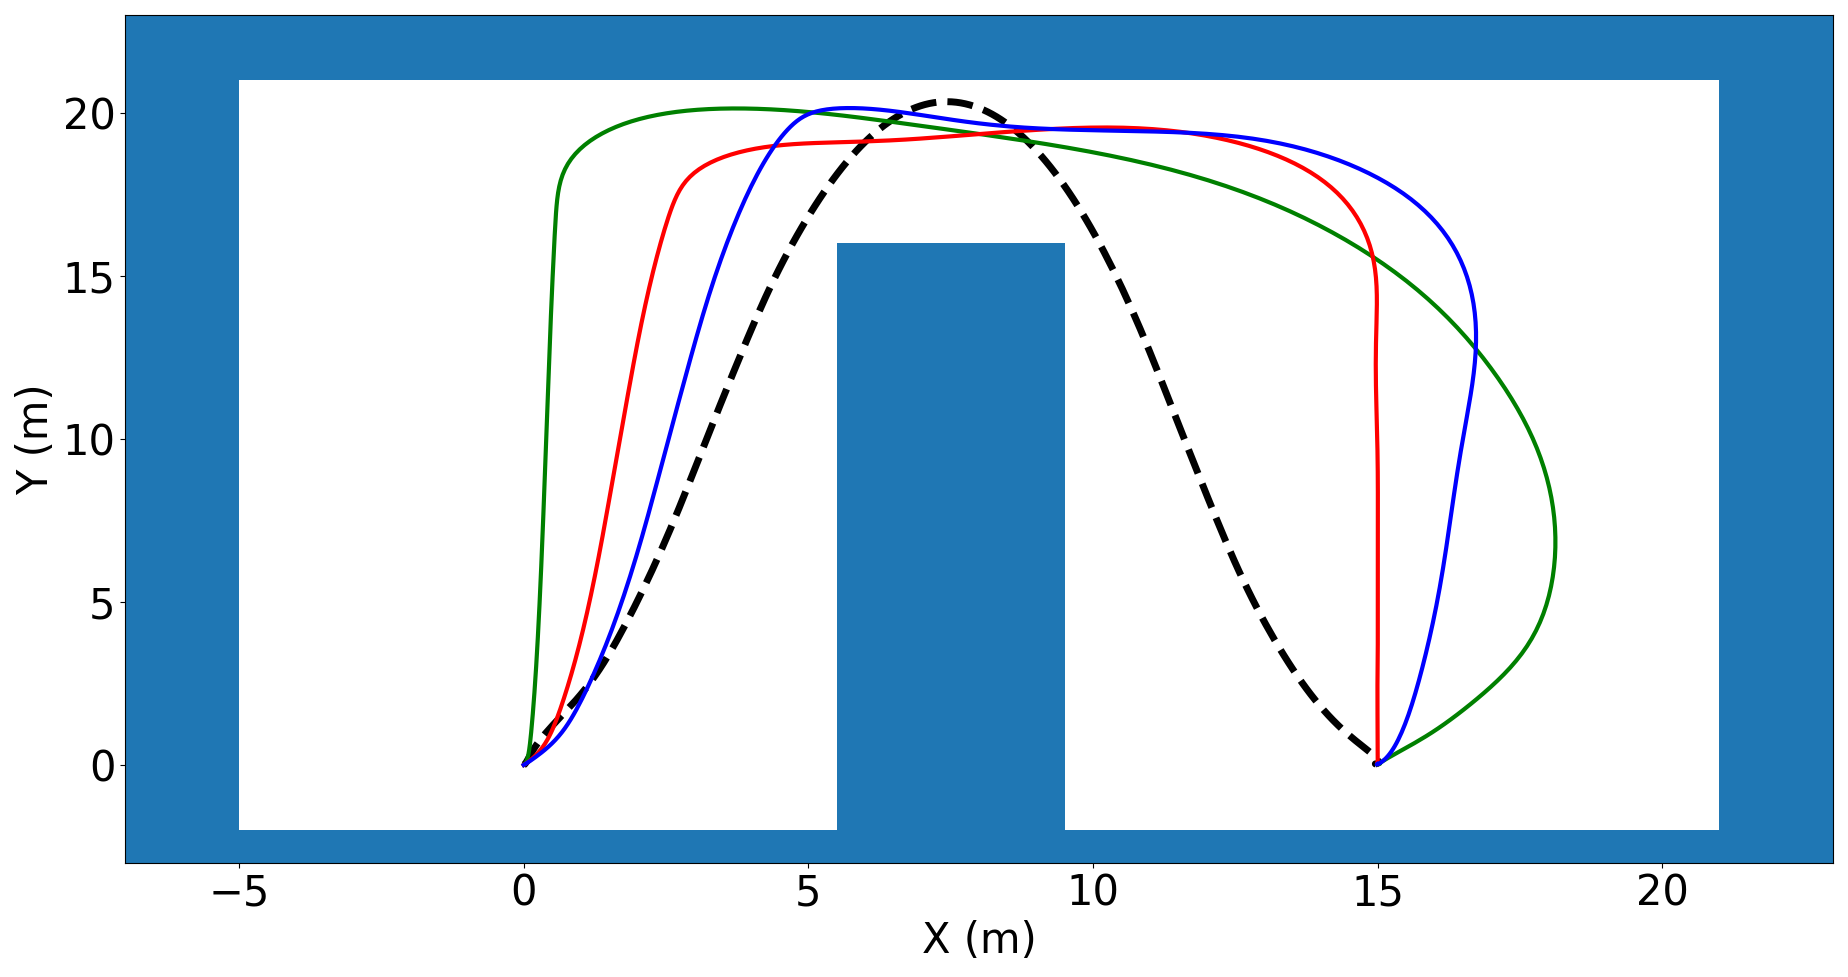
\includegraphics[width=0.7\linewidth]{figures/samp/U_shape_3in1_before.png}
    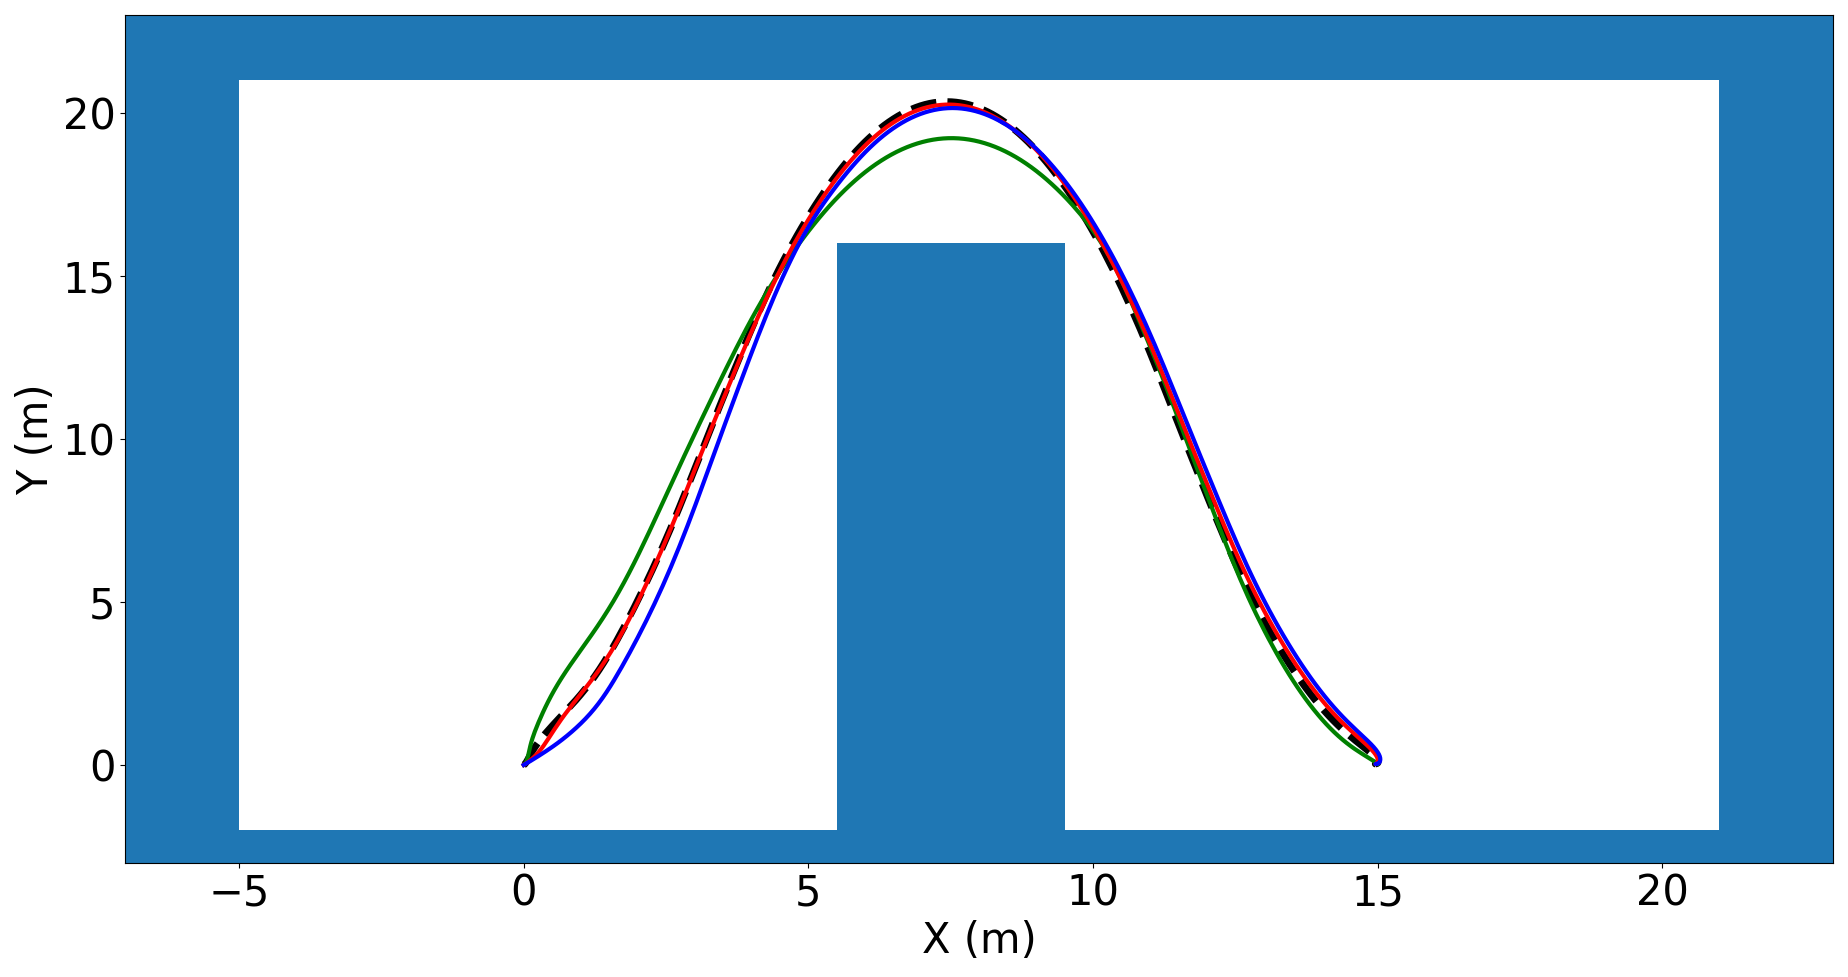
\includegraphics[width=0.7\linewidth]{figures/samp/U_shape_3in1_after.png}
    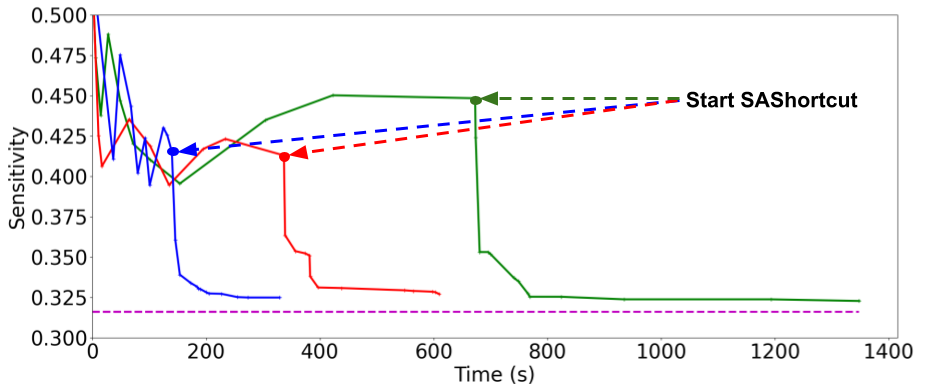
\includegraphics[width=0.7\linewidth]{figures/samp/U_shape_3in1_sensi.png}
    \caption{Three trajectories (red, green, blue) produced by \myglsentry{lazysarrt*} (top), and the three trajectories resulting from \myglsentry{SAshortcut} (middle), with the evolution of their respective sensitivity (bottom). 
    The dashed black trajectory (top, middle) and the dashed purple cost (bottom) correspond to the sensitivity-optimal reference found using the \myglsentry{sasst*}.}
    \label{fig:U_shape}
\end{figure}

Figure~\ref{fig:U_shape} shows how the decoupled approach is able to produce solutions that mimic the optimal one found by the \myglsentry{sasst*} in the so called U-shape environment considering the $\delta\p_{low}$ parametric uncertainty vector.
Furthermore, according to the results shown in Table~\ref{tab:lazySAMP_quad} and in Figure~\ref{fig:U_shape}, \myglsentry{SAshortcut} produces solutions with sensitivity costs close to the optimal reference found by \myglsentry{sasst*}. 
Also note the huge time saving of the proposed method compared to the \myglsentry{sasst*}.
Additionally, note that during the \myglsentry{lazysarrt*} planning, the trajectory length optimization allow to decrease the sensitivity cost although this was not the objective function, comforting the choice of a (near) time-optimal as an initial guess for the \myglsentry{SAshortcut} and the use of a length metric as a state space metric when optimizing the sensitivity within the \myglsentry{sarrt*} and \myglsentry{sasst*} of Section~\ref{sec:samp_simu}.

Finally, note that the average computing time of \myglsentry{lazysarrt*} in this case is low compared to the other environments. 
This is mainly due to the fact that in this case the time-optimal trajectory is far from the obstacles and therefore few re-connections via the \myglsentry{lazysarrt*} RobustReconnect procedure are performed when extending the tree.

\paragraph{2D 2-way Environments} 

\begin{figure}[t]
    \centering
    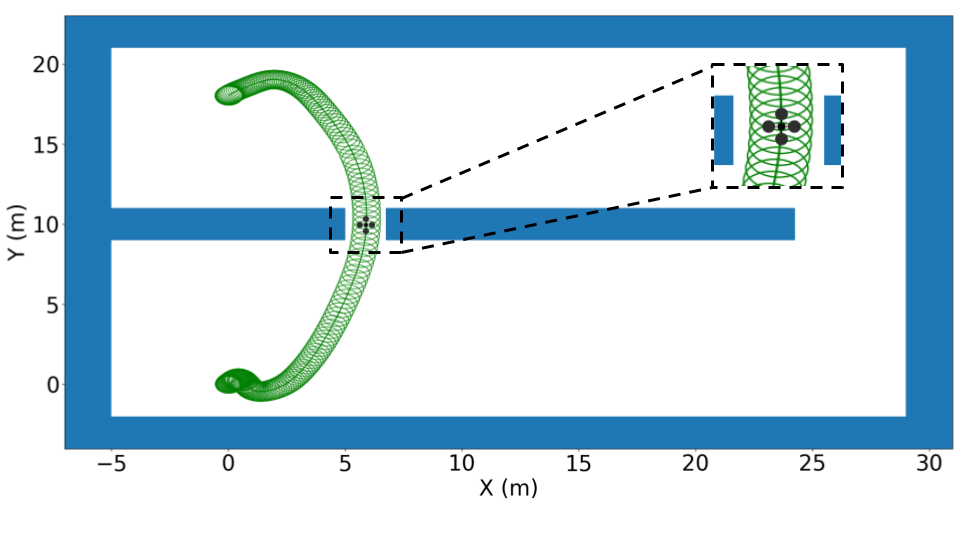
\includegraphics[width=0.7\linewidth]{figures/samp/Contribution-example1.png}
    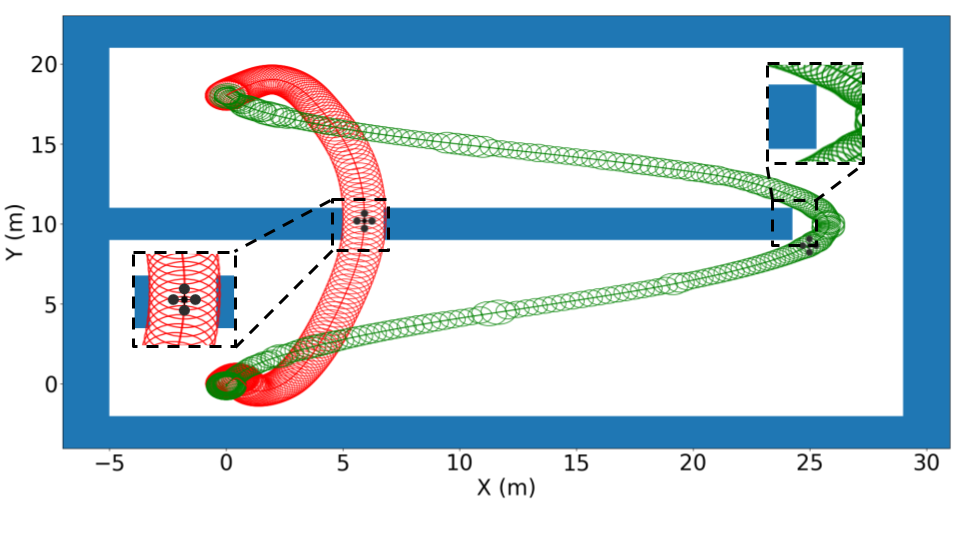
\includegraphics[width=0.7\linewidth]{figures/samp/Contribution-example2.png}
    \caption{Solutions with their uncertainty tube (in green) computed by the decoupled approach between the same start/goal states of a quadrotor dynamical model for small/high parameters uncertainties (top/bottom, respectively)}
    \label{fig:2way}
\end{figure}

This environment referred to Figure~\ref{fig:2way} where the two sets of uncertainties $\delta\p_{low}$ and $\delta\p_{high}$ are considered.

As shown in Figure~\ref{fig:2way}, in the presence of small uncertainties the decoupled approach produces a trajectory allowing to use the narrow passage. 
However, while considering large uncertainties, the time optimal trajectory which goes through the narrow passage cannot be taken as a collision is found by considering the uncertainty tube as shown in red in the Figure~\ref{fig:2way}.
Nevertheless, SAMP is able to find the fastest trajectory apart from those passing through this passage.

In both cases the average cost of the solutions produced by SAMP is close to that found by \myglsentry{sasst*} as shown in Table~\ref{tab:lazySAMP_quad}, where 2-Way$_{low}$ refers to the presence of small uncertainties and 2-Way$_{high}$ to the presence of large uncertainties.
The average computing time of the \myglsentry{sasst*} is equivalent in both cases as it is performed on exactly the same environment.
However, note that the average computing time of the \myglsentry{lazysarrt*} is longer than in the U-shape case because the time-optimal trajectories must pass through a location where many collisions may occur. 
Moreover, in the 2-Way$_{high}$ case the \myglsentry{lazysarrt*} computing time is longer than in the 2-Way$_{low}$ as even more non-robust trajectories are found.
This is because more iterations are needed before considering a neighborhood deprived of nodes passing through the narrow corridor.
Finally, we see that the \myglsentry{SAshortcut} computing time remains of the same order of magnitude for both cases as that of the U-shape, and again SAMP produces a solution much faster than \myglsentry{sasst*}.

\paragraph{3D Environment} 

\begin{figure}[t]
\centering
    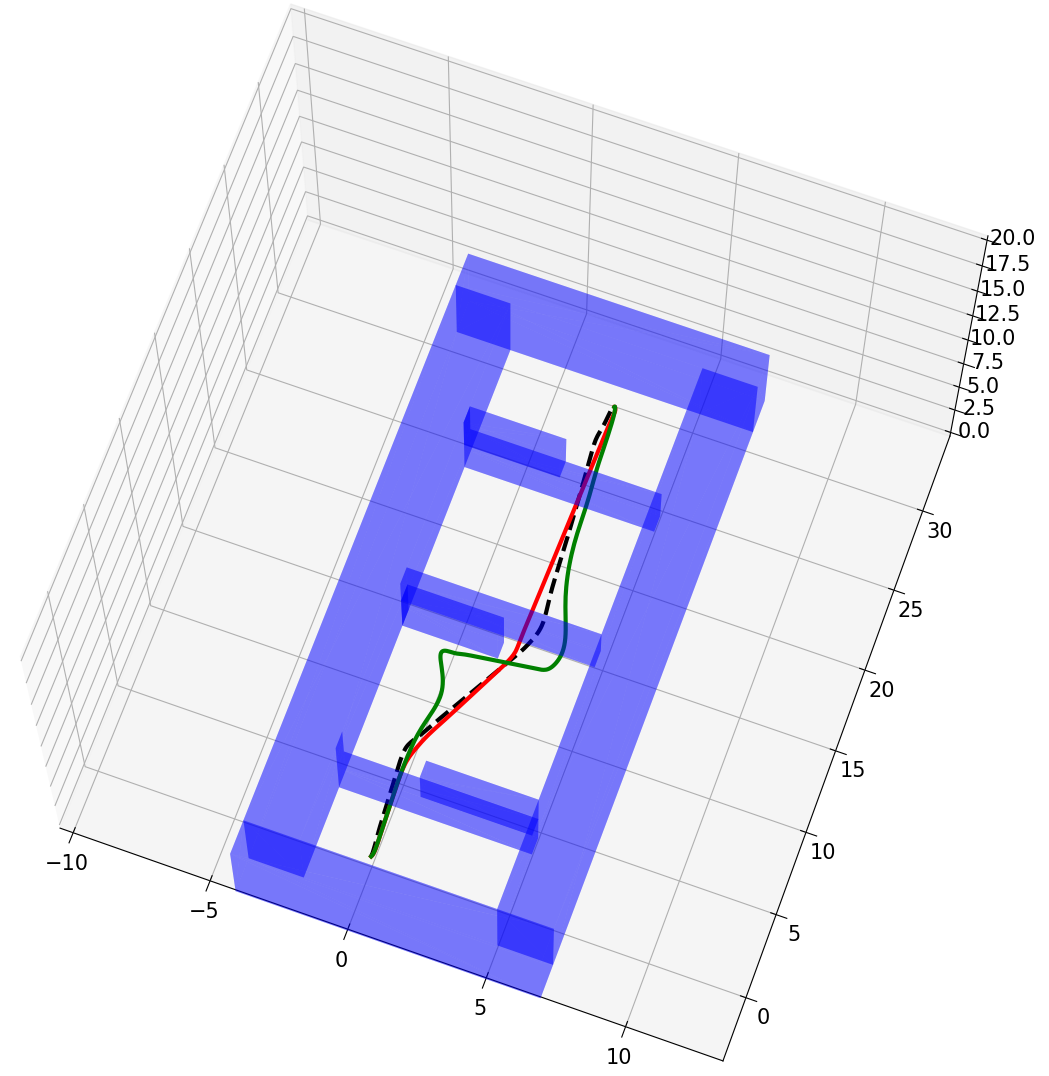
\includegraphics[width=0.7\linewidth]{figures/samp/3D_full_view.png}
    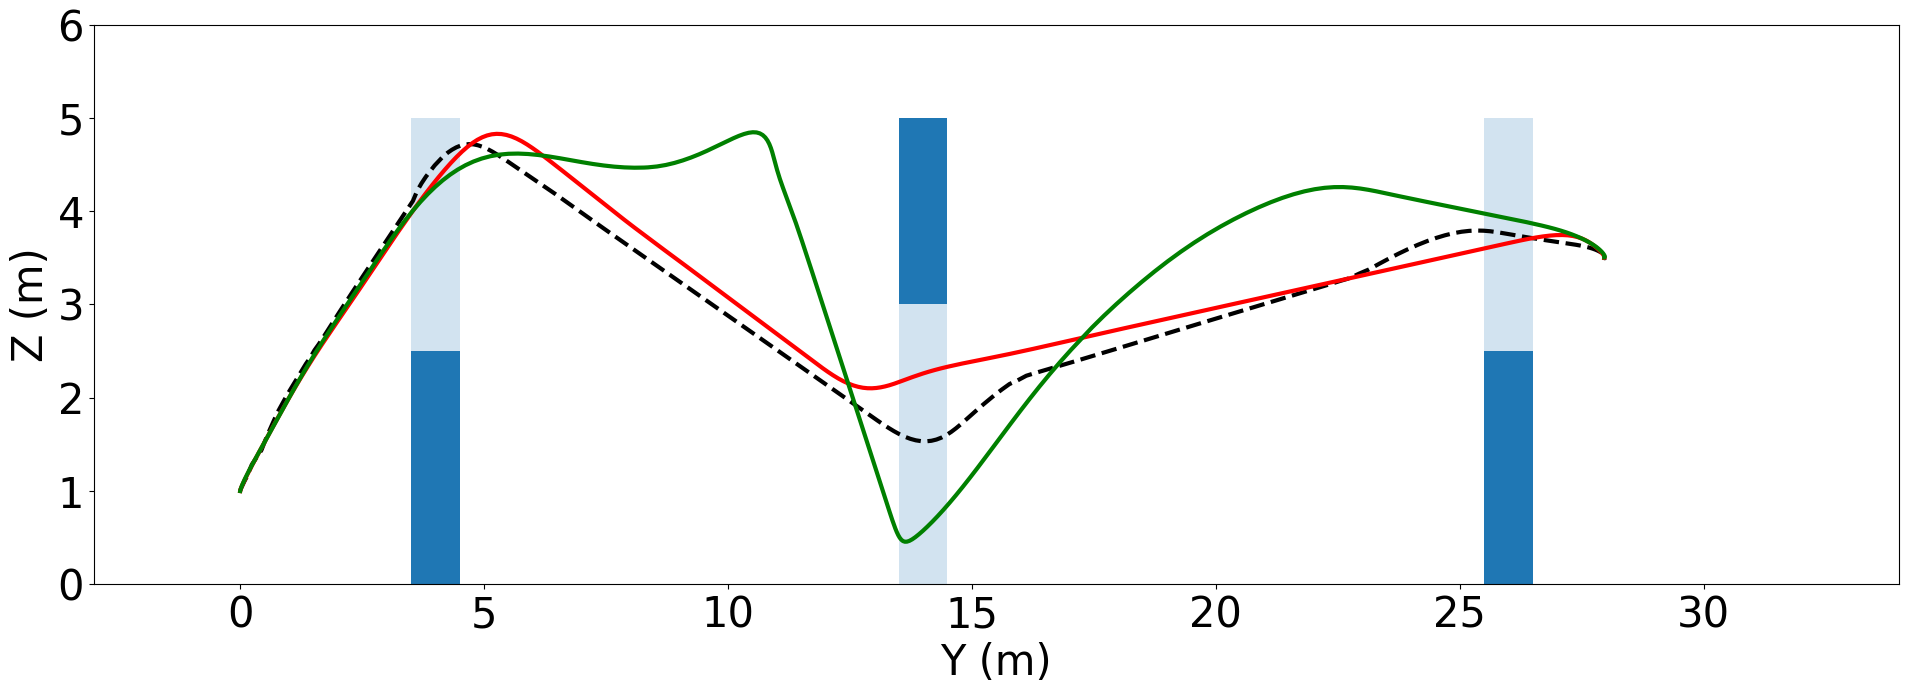
\includegraphics[width=0.7\linewidth]{figures/samp/3D_ZYprofile.png}
    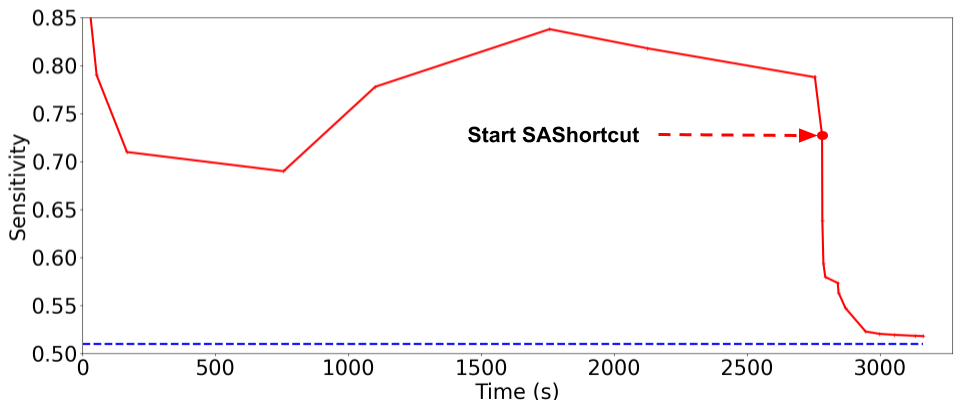
\includegraphics[width=0.7\linewidth]{figures/samp/3D_sensi.png}
    \caption{Trajectories produced by \myglsentry{lazysarrt*} (green), SAMP (red), and \myglsentry{sasst*} (dashed black) in a 3D environment (top). A profile view along the YZ plane is given (middle) as well as the evolution of the sensitivity (red) and the optimal one found by the SST$^*$ (dashed blue) (bottom) during the execution of SAMP.}
    \label{fig:3D}
\end{figure}

The uncertainty set considered in this full 3D environment is $\delta\p_{low}$.
As shown in Figure~\ref{fig:3D}, once again the decoupled approach produces trajectories that mimic the optimal obtained by the \myglsentry{sasst*}.
It is interesting to note the impact of the \myglsentry{SAshortcut} procedure on the Z component in addition to the impact on the X Y components already seen in the previous 2D environments.
The average computing time of the shortcut is similar to other environments according to Table~\ref{tab:lazySAMP_quad}.
Again, the SAMP method produces a near-optimal trajectory much faster than conventional optimal planners.

\section{Conclusion}\label{sec:concl}
Note that the algorithms not complete proof

Approach more efficient when we reduce the number of call. 

Additionally, one may compute the ODEs for unbounded local trajectories. 
Leading to high computation times for most of the time unfeasible local trajectories. 
Based on OMPL implementation we chose to use maximum local trajectories length.
\todomarker[]{graph RSARRT* with unbounded length and bounded length, to show that we reduce the part of the ODEs but that still need to improve ODEs solvers computation time, cf learning}

However, we still need to improve the computation time.

% \cleardoublepage
% \newpage 
% \ % The empty page
% \newpage
\chapter{Learning uncertainty tubes via recurrent neural networks} \label{chap:NN}
\markboth{Learning uncertainty tubes via recurrent neural networks}{}% To set left/right header
% \localtableofcontents

% Parallelization of ODE (Ordinary Differential Equations) solvers for systems like a quadrotor is indeed possible, but it comes with certain challenges due to the inherent sequential nature of ODE solvers. Each time step generally depends on the previous one, making it difficult to parallelize directly. However, various techniques and strategies can help in parallelizing ODEs, even for small time steps. Let's explore this in more detail.
% 1. Parallelization in ODE Solvers

% ODE solvers like Runge-Kutta, Euler, or Adams-Bashforth typically compute solutions in a time-stepping manner, where each step depends on the solution from the previous step. This sequential dependency makes it hard to directly parallelize time integration.

% However, some strategies can parallelize parts of the problem:
% 1.1 Parallelizing the Evaluation of Derivatives

% The right-hand side (RHS) of the ODE system (i.e., the function that describes the system's dynamics) can often be parallelized if it involves multiple independent computations. For example, in a quadrotor, if the dynamics involve complex matrix operations, vector algebra, or sensor models, these computations can be parallelized across multiple cores or even on a GPU.
% 1.2 Domain Decomposition for Parallelization

% This approach involves splitting the physical domain or the variables of the system and solving them in parallel. For a quadrotor, domain decomposition may not apply as easily as it would for a large physical domain problem (like fluid dynamics), but it could still be used if the quadrotor's dynamics are complex and involve interacting subsystems. For instance, rotor dynamics, attitude control, and position dynamics could potentially be solved in parallel if they are weakly coupled.
% 1.3 Multiple Shooting or Parareal Algorithms

% These methods introduce parallelization by splitting the time domain into multiple intervals and solving the ODE in parallel on each subinterval.

%     Parareal Algorithm: This method allows for parallel time integration by solving coarse approximations over large time intervals in parallel, followed by corrections using fine time steps. While the fine steps remain sequential, the coarse steps can be parallelized. The Parareal method is well-suited for large-scale systems but might be overkill for small systems like a quadrotor, especially with small time steps.

%     Multiple Shooting: In this technique, the time domain is divided into smaller intervals, and the ODE is solved independently in each interval. The solutions are then stitched together using boundary conditions. This method is typically used for stiff ODE problems or optimization-based control (like Model Predictive Control).

% 1.4 Parallel Integration of Different States

% In some cases, the state variables of a system might evolve independently or with weak coupling, allowing for parallel integration of different states. For a quadrotor, some aspects of the dynamics (e.g., attitude and position) could potentially be integrated separately in parallel, especially if the time scales are slightly different.
% 2. Time-Stepping Constraints and Relaxation

% You mentioned time-step constraints. In ODE solvers, especially explicit solvers like Runge-Kutta or Euler, the time step size is usually limited by stability constraints (e.g., Courant-Friedrichs-Lewy (CFL) condition for PDEs or step size for stiff ODEs).

%     Relaxing Time-Step Constraints: Parallelization techniques like Parareal introduce time-step relaxation by allowing coarse-grain parallel computations over larger time intervals, then correcting with smaller steps sequentially. This is useful for accelerating convergence in large-scale simulations with longer time horizons.

%     Using Small Time Steps in Parallelization: If your goal is to maintain small time steps (e.g., for accuracy, stability, or real-time control in a quadrotor), relaxation-based methods might not be as helpful. However, parallelization can still help in other ways:
%         Task-based Parallelism: Use parallel computing resources to speed up the evaluation of forces, torques, control inputs, sensor models, or optimization procedures (if using real-time control).
%         Predictor-Corrector Methods: These methods can use a fast, coarse-grained predictor step, followed by parallel corrections that refine the solution. The corrections can be done in parallel with small time steps, making it more suitable for small time steps.
%         Parallelization of Subsystems: Parallelizing distinct components of the quadrotor's dynamics (e.g., thrust dynamics, rotational dynamics, or environmental interactions) can improve computational efficiency while keeping the same small time steps.

% 3. Maintaining Small Time Steps in Parallelization

% To directly answer your question, you can use parallelization techniques while keeping small time steps, but the degree of parallelization might be more limited compared to approaches where time steps are relaxed. The most promising approaches in this scenario would be:

%     Parallel evaluation of the system's dynamics: Evaluating the dynamics (i.e., the forces and moments) in parallel could reduce computation time significantly, especially if your quadrotor model involves complex dynamics (e.g., aerodynamic drag, rotor dynamics, etc.).

%     Task-level parallelism: In real-time control applications, parallelizing sensor fusion, state estimation, and control computations (while maintaining small time steps) can improve performance.

%     Multiple shooting methods: Even with small time steps, the multiple shooting method can potentially parallelize certain segments of the time domain, but you'd need to stitch together the results carefully, ensuring stability.

% Conclusion

% While parallelization techniques like Parareal or Multiple Shooting often involve relaxing time-step constraints, it is still possible to parallelize certain parts of the quadrotor's ODE solver without relaxing the small time-step constraints. You can achieve this by focusing on parallelizing the evaluation of the system's dynamics, using task-level parallelism, or exploiting weakly coupled subsystems. However, the benefit of parallelization will likely be more constrained compared to systems where time-step constraints are relaxed.

% 3. Challenges of Using Parareal for Control Stability

% The Parareal method works by first running a coarse-grained simulation with larger time steps, followed by corrections using finer time steps. If the coarse solver uses large time steps, it could violate the control stability requirements during the initial stages of the Parareal iterations. This would make it unsuitable for real-time control if the initial approximation (coarse solver) is far from accurate, as the control system relies on frequent updates.



% Your GRU (Gated Recurrent Unit) neural network might be faster than other methods for solving an ODE on a CPU for several reasons related to its structure and the way neural networks handle data. The efficiency of GRU in this context largely depends on the number of operations it performs and how well it's optimized for CPU computations. Let's break it down:
% Why GRU is Faster for ODE Solving on CPU:

%     Fewer Parameters: GRUs are known for their simplicity compared to other recurrent neural networks (RNNs) like LSTMs. GRUs have fewer gates and parameters, making them computationally cheaper.
%         GRUs have only two gates (reset and update), while LSTMs have three gates (input, forget, output), which translates to fewer matrix multiplications per time step.
%         Fewer parameters also mean less memory consumption, which reduces the computational load when training or running the model.

%     Parallelism: Neural networks, including GRUs, can be structured in such a way that they process multiple data points (or time steps) in parallel, especially during training or inference. This can make GRUs more efficient than traditional methods for solving ODEs, such as Runge-Kutta, which might be more sequential in nature.

%     Reduced Complexity of Time-Stepping:
%         Numerical methods for solving ODEs, such as Runge-Kutta or implicit methods, often involve multiple function evaluations at each time step. GRUs, however, learn a representation of the system's dynamics, effectively "learning" a function approximation, which can be faster at runtime.
%         GRUs can use a single pass per time step (or batch of time steps), while traditional solvers may require many steps or iterations at each point.


% Model Type	Inference Time	Remarks
% RNN (GRU, LSTM)	Faster	Efficient for discrete, regular time steps; fixed computation per time step
% Neural ODE	Slower	Inference depends on ODE solver complexity and system dynamics

% In most practical scenarios, RNNs (GRUs, LSTMs) will offer faster inference compared to Neural ODEs due to the absence of ODE solvers and the simpler, more direct nature of their computations. Neural ODEs are more suited for scenarios where continuous dynamics are the priority, but this often comes at the cost of slower inference times.

% Time Steps vs. ODE Solver Integration:

%     In RNNs, the number of time steps is fixed, and you perform one forward pass per time step.
%     In Neural ODEs, the time steps are determined by the ODE solver, which can be adaptive. The solver may take many small steps or fewer large steps, depending on the system's complexity.

%     RNNs (GRU, LSTM, etc.):

%     RNNs are designed to handle discrete time sequences. They take input in the form of a time series with fixed time steps (e.g., t1,t2,t3,...) and learn to map these discrete states over time.
%     RNNs operate by passing hidden states from one time step to the next, effectively modeling the temporal correlations in the data.
%     LSTMs and GRUs are specific variants of RNNs that improve on the basic RNN structure by addressing the problem of vanishing/exploding gradients in long sequences. They do this using gating mechanisms that control the flow of information through time.
%     Since RNNs work with fixed time steps, they model time as discrete, and handling continuous dynamics requires fine-tuning, such as choosing a time step size.

% Neural ODEs:

%     Neural ODEs, on the other hand, model continuous-time dynamics. They replace the discrete sequence of states (as in RNNs) with a differential equation for the hidden states:
%     dh(t)dt=f(h(t),t,θ)
%     dtdh(t)=f(h(t),t,θ) where ff is a neural network and θθ are its parameters. The dynamics evolve continuously over time, and you can evaluate the state at any arbitrary time tt, not just at predefined discrete steps.
%     Neural ODEs use ODE solvers to numerically integrate the system over time, allowing for flexible handling of varying time steps and even irregular or non-uniform time intervals.


% The use of a simple GRU architecture instead of Neural ODEs or Physics-Informed Neural Networks (PINNs) to approximate ODE solutions in the context of the paper by Wasiela et al. likely stems from several practical advantages that GRUs offer, particularly in the domain of real-time robot motion planning and control. Here are the key reasons and advantages of this choice:
%     1. Efficiency and Simplicity in Real-Time Applications
    
%     GRUs are known for their computational efficiency, especially in real-time applications like robotics where fast decision-making is crucial. A GRU-based model can be trained relatively easily and deployed quickly for inference, allowing the robot to plan and adjust its motions on the fly.
    
%         Fewer Parameters: Compared to models like Neural ODEs or more complex recurrent architectures, GRUs have a simpler structure and fewer parameters, making them faster and more efficient during inference. This makes GRUs particularly well-suited for tasks where real-time performance is required, such as robot motion planning.
    
%     2. Handling Sequential Data with Temporal Dependencies
    
%     GRUs are designed to handle sequential data and are efficient at modeling temporal dependencies, which are common in dynamical systems. In the context of approximating ODEs for robot motion, where states evolve over time, GRUs can track the evolving state of the robot and make predictions about future states efficiently.
    
%         Unlike Neural ODEs, which require solving differential equations iteratively through a solver, GRUs can directly approximate the state transitions (i.e., how the system evolves in time) in a single forward pass per time step, making them faster for inference.
    
%     3. Avoiding the Complexity of ODE Solvers
    
%     Neural ODEs, while powerful, often rely on the use of ODE solvers during training and inference, which can be computationally expensive and require adaptive step sizes. These solvers often need to balance accuracy with computational speed, which can become a bottleneck in real-time applications.
    
%         GRUs, in contrast, do not require iterative solvers to propagate forward in time. Once trained, a GRU can generate the next state in the sequence in a single step, leading to much faster performance, especially in resource-constrained environments like robotics.
    
%     4. Flexibility and Generalization
    
%     GRUs are flexible in terms of what kind of sequential data they can handle. Unlike Physics-Informed Neural Networks (PINNs), which integrate physical constraints directly into the learning process (requiring knowledge of the system’s physics and explicit boundary conditions), GRUs can approximate ODEs without needing explicit knowledge of the underlying physical laws.
    
%         This makes GRUs a more flexible and practical choice when the goal is to approximate the system’s behavior based on empirical data, rather than being strictly bound to physical laws or differential equations. This is especially useful in real-world scenarios where the system dynamics may be complex or partially unknown.
    
%     5. Data-Driven Approach with Learned Dynamics
    
%     In applications where data-driven approaches are preferred (such as when the robot's environment is highly dynamic or uncertain), GRUs can learn to model the system’s dynamics based purely on input-output data without needing a detailed mathematical model.
    
%         Neural ODEs and PINNs require knowledge of the system’s governing equations (or their differential form), which may not always be available or easy to define in the context of robot motion planning with uncertainties. A GRU can capture complex non-linear dynamics without needing to explicitly model the differential equations.
    
%     6. Handling Uncertainty and Robustness
    
%     In the paper, the GRU is used to model Learned Uncertainty Tubes, which suggests that the authors are dealing with uncertain environments and need a way to account for this uncertainty in planning robust robot motions. GRUs are good at capturing uncertainty in sequential predictions because of their inherent ability to model and propagate information over time.
    
%         GRUs can be trained to model not just the system's trajectory, but also the potential deviations or uncertainties in future states. This allows the GRU-based model to handle uncertain environments more robustly and efficiently, which may be harder to achieve with Neural ODEs or PINNs due to the complexity of integrating uncertainty into those frameworks.
    
%     7. Empirical Success and Ease of Implementation
    
%     Another reason for choosing GRUs could simply be their empirical success in time-series forecasting and modeling dynamic systems. They are widely used and have proven to work well in practice. Additionally, GRUs are easier to implement and train compared to Neural ODEs or PINNs, which often require more sophisticated training setups, custom loss functions, and solvers.
%     Summary of Advantages of Using GRUs over Neural ODEs or PINNs:
    
%         Faster inference: GRUs don't need iterative ODE solvers, making them more efficient for real-time applications.
%         Simplicity: GRUs are simpler to implement and require fewer resources compared to Neural ODEs or PINNs.
%         Good at handling sequential data: GRUs excel at modeling time-series data and can approximate temporal dependencies effectively.
%         Data-driven and flexible: GRUs can approximate the dynamics of a system without needing a detailed mathematical model of the underlying physics.
%         Handling uncertainty: GRUs are well-suited for modeling uncertainty in robot motion planning, as they can track evolving dynamics and uncertainties over time.
    
%     By using GRUs, the authors likely balance between achieving real-time performance, modeling complex dynamics, and managing uncertainties—all essential for robust robot motion planning.

%     You're absolutely right. Since the authors in the mentioned paper want to bypass the ODEs and avoid calling traditional solvers (like Euler, Runge-Kutta, etc.), Neural ODEs (NODEs) are not suitable because NODEs inherently rely on ODE solvers during inference. Let's now consider whether Physics-Informed Neural Networks (PINNs) could be an alternative, given the situation.
%     Why PINNs Might Not Be the Right Fit in This Context
    
%     Even though PINNs integrate known ODEs into the learning process, there are several reasons why they might not be the best choice for this particular case where the authors want to completely bypass the ODEs:
    
%     2. PINNs May Not Be as Efficient in Real-Time
    
%         PINNs often require more computational resources and longer training times because they solve ODEs in a way that enforces the governing equations (through residuals and constraints). This can lead to slower inference times compared to using something like a GRU, which is purely data-driven and bypasses both the explicit and implicit use of ODEs.
    
%         In the context of robot motion planning—which requires fast, real-time predictions—PINNs might be overkill or too computationally demanding for the purpose, especially when the focus is on efficient approximation of motion without solving differential equations explicitly.
    
%     3. PINNs Are Better Suited When Physics Constraints Are Critical
    
%         PINNs excel when you want to incorporate physical constraints or laws explicitly during learning, particularly when data is sparse or noisy. However, in the case where the authors want to approximate the ODEs using a simple data-driven approach (like a GRU), it suggests that they are prioritizing speed and simplicity over strict adherence to the physics.
    
%         If the authors are confident that the GRU can capture the dynamics without relying on the exact physical laws during inference, then the use of PINNs—which are designed to enforce those physical laws—becomes unnecessary.

\section{Reccurent neural networks: overview}

\section{Method} \label{sec:method}
\subsection{Problem statement}
\subsection{Neural network architecture}
\subsection{Dataset}

\section{Evaluation}
\subsection{Metrics}
\subsection{Implementation details}

\section{Simulation results}
\subsection{Training}
\subsection{Model comparison}
\subsection{Ablation study}
\subsection{Qualitative results}

\section{Conclusion} \label{sec:concl}

\todomarker{}
% \cleardoublepage
% \newpage 
% \ % The empty page
% \newpage
\chapter{Robust motion planning with accuracy optimization based on learned sensitivity metrics}[TOTO]
\markboth{Robust motion planning with accuracy optimization based on learned sensitivity metrics}{TITI}% To set left/right header
% \localtableofcontents

\section{Introduction} \label{sec:introduction}

To overcome some of the aforementioned problems, the sensitivity-aware motion planner (SAMP) proposed in~\cite{cSAMP} exploits the derivation of uncertainty tubes of \cite{cTube}, based on the so-called \emph{closed-loop sensitivity}~\cite{cPi,cTh}.
This approach is applicable to any controller and robot model, taking into account parametric uncertainties. 
However, this planner suffers from the high computational cost of computing the uncertainty tubes.
Moreover, SAMP and the aforementioned methods focus on computing robust trajectories but do not consider the problem of \emph{also} minimizing uncertainty tubes at a desired location for increasing the accuracy of specific tasks (e.g., insertion, grasping).

\begin{figure} [t]
    \centering
    \subfloat[\centering Robust motion planning]{{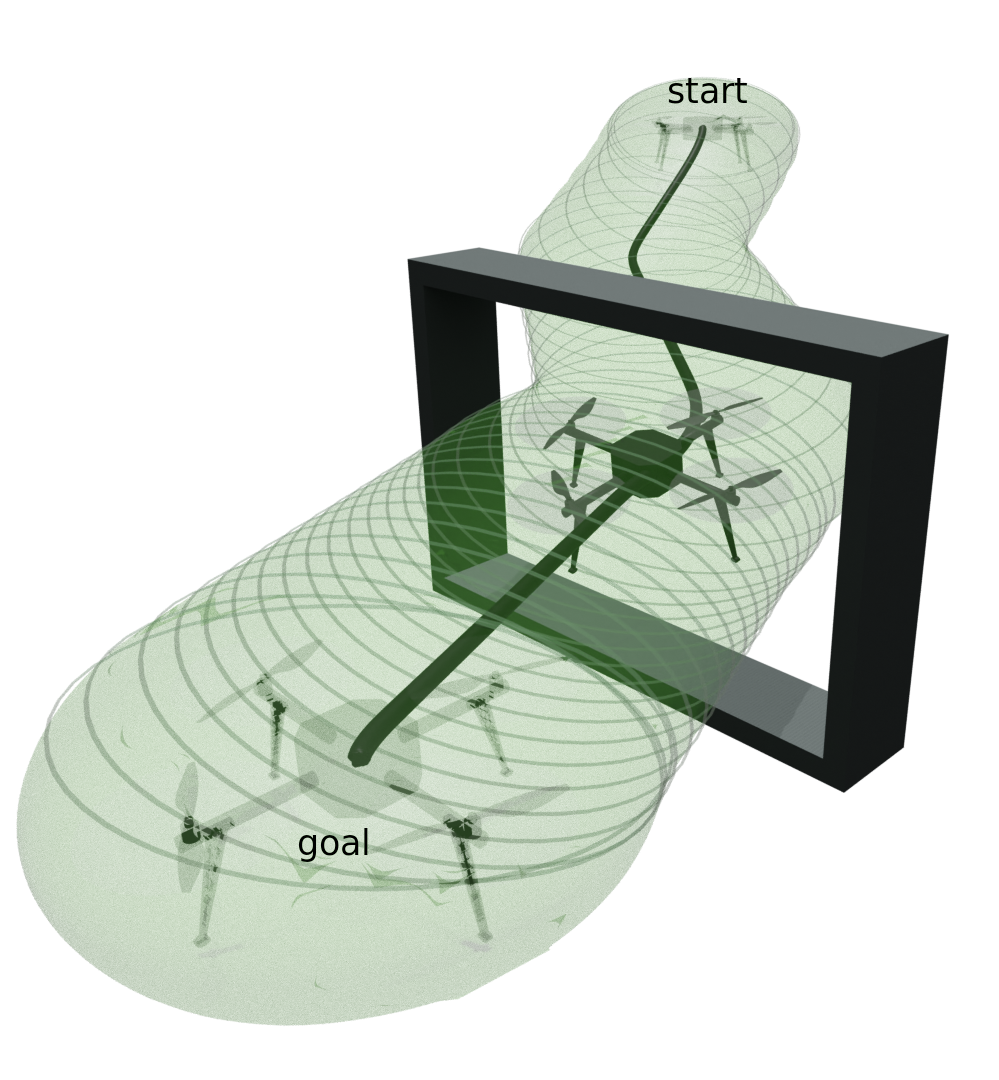
\includegraphics[width=0.4\linewidth]{figures/robust_accurate/topFig_tube.png} }\label{fig: fig1robust}}%
    \subfloat[\centering Accuracy optimization]{{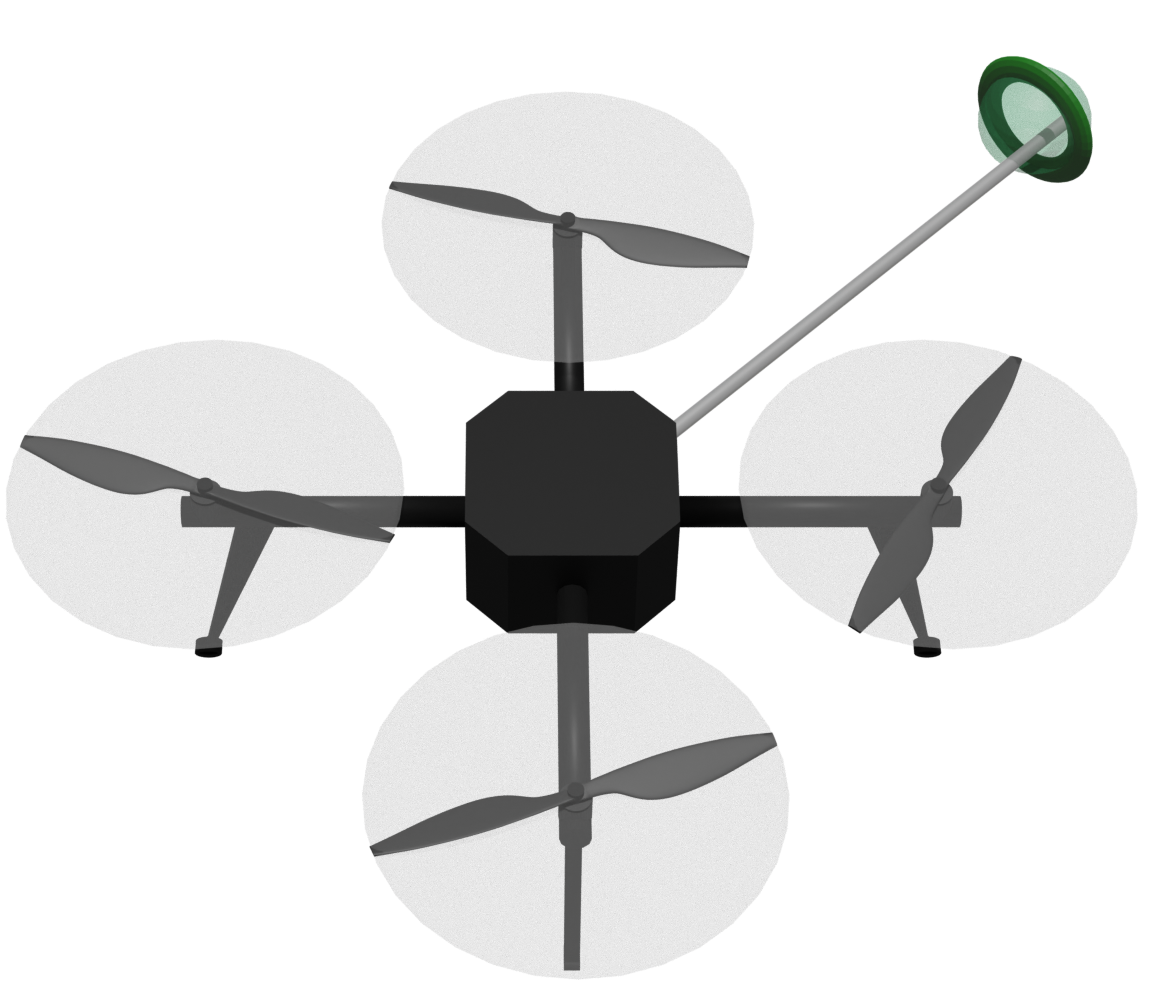
\includegraphics[width=0.4\linewidth]{figures/robust_accurate/ring_success.png} } \label{fig: fig1acc}}%
    \caption{
    Two scenarios considered for the experimental validation of the proposed method:
    (a) Robust navigation of a drone through a narrow window. (b) Precision in-flight `ring catching' task, where the uncertainty on the position of the perch end-effector is minimized to successfully accomplish the task.
    A video of the experiments is available at: \href{https://laas.hal.science/hal-04642257}{https://laas.hal.science/hal-04642257} \vspace{-0.4cm}}%
    \label{fig: Missed and succes}%
\end{figure}

With respect to these considerations, the contribution of this paper is twofold:
(i) We propose a computationally efficient version of the SAMP algorithm,
relying on a Gated Recurrent Unit neural network (GRU)\cite{cGRU} (see Chap.~\ref{chap:NN}), which quickly and accurately estimates time-varying uncertainty tubes and control input profiles along trajectories.
We present a general way of incorporating this type of network into a sampling-based tree planner in order to predict the uncertainty tubes and control inputs along trajectories. 
(ii) On the basis of this new planner, 
we propose a comprehensive framework that not only plans robust trajectories but also locally optimizes them together with the controller gains to maximize accuracy at some desired states of the planned trajectory for any system/controller.

Fig.~\ref{fig: Missed and succes} illustrates the application to a quadrotor model in two different experimental scenarios involving uncertain parameters affecting the robot model (see Sect.\ref{sec:Simu Results}): (i) a robust navigation through a narrow window;
(ii) an in-flight ring-catching task demonstrating the robustness and accuracy of the proposed framework. 

% Sect.~\ref{sec:RASAMP} provides an overview of our planning framework to generate robust and accurate trajectories.
% Sect.~\ref{sec:RSAMP} shows how to integrate the sensitivity learning method within a sampling-based motion planner, while Sect.~\ref{sec:AOptim} explains the accuracy optimization stage.

\subsection{Robust and accurate planning framework}\label{sec:RASAMP}

The method consists of two stages: $(i)$ first, it generates a robust trajectory based on a Robust Sensitivity-Aware Motion Planner (R-SAMP) -- explained in Sect.~\ref{sec:RSAMP} -- that utilizes the GRU-based computation of the uncertainty tubes; $(ii)$ second, it optimizes the accuracy at some given states along this trajectory by minimizing the size of the uncertainty tubes at these locations.
The motivation behind the second stage is to improve the accuracy of the planned robust trajectory for tasks -- e.g., pick-and-place or insertion tasks -- where minimizing the deviation from the nominal trajectory is important only at specific designed locations, as for picking the ring in Fig.~\ref{fig: Missed and succes}.

The pseudo-code of RA-SAMP (Robust and Accurate Sensitivity-Aware Motion Planner) is presented in Alg.\ref{alg:RA-SAMP}. 
It takes as input (line 1) a list of desired states $list_{d} = (q_{d}^0, \dots, q_{d}^n)$ for which the accuracy should be optimized, and the initial controller gains vector $k_{c}^{init}$ considered constant all along the trajectory.

\begin{algorithm}[h]
\caption{RA-SAMP [$list_{d}, k_{c}^{init}$]}\label{alg:RA-SAMP}
\begin{algorithmic}[1]
\State $\pi_d^{tot} \gets \emptyset;$
\For {($i=1;\ i< len(list_{d});\ i=i+1$)}
    \State $\pi_d^{tot} \gets \pi_d^{tot} + $R-SAMP$(list_{d}(i-1),list_{d}(i));$
\EndFor
\State $\left \{ \pi_d^{tot}, k_{c}^{opt} \right \} \gets $A-Optim$(list_{d},\pi_d^{tot}, k_{c}^{init});$
\State \textbf{return} $\left \{ \pi_d^{tot}, k_{c}^{opt}  \right \}$;
\end{algorithmic}
\end{algorithm}

The first step of the algorithm consists of generating robust trajectories ($\pi_d^i$) between successive desired states in the list (line 3 of Alg.~\ref{alg:RA-SAMP}) by means of a robust sensitivity-aware motion planner called R-SAMP (explained in Sect.~\ref{sec:RSAMP}) that uses our learning approach.
These trajectories are concatenated into a global one $\pi_d^{tot}$, connecting all the desired states of $list_{d}$ (lines 2-5 in Alg.~\ref{alg:RA-SAMP}). 

The trajectory from R-SAMP is locally modified by A-Optim (line 6 in Alg.~\ref{alg:RA-SAMP}), aiming at optimizing the accuracy at specific desired states along the trajectory. 
This algorithm iteratively samples both the trajectory from R-SAMP and the controller gains, adjusting the former to minimize uncertainty at these states. 
Indeed, as demonstrated in \cite{AliIROS}, optimizing both factors concurrently results in minimizing the uncertainty.
The algorithm produces two offline outputs: $(i)$ a robust desired trajectory $\pi_d^{tot}$ optimized for accuracy at the desired states, and $(ii)$ the optimized controller gains vector $k_{c}^{opt}$, considered constant throughout the trajectory.

\subsection{Robust Sensitivity-Aware Motion Planner}\label{sec:RSAMP}

This section explains how the learned uncertainty tubes can be incorporated into any sampling-based tree planner in order to obtain a robust sensitivity-aware motion planner (R-SAMP).
As highlighted before, a key challenge in computing such tubes for a given trajectory lies in the high computational cost of numerically integrating the dynamics of $\bPi(t)$ and $\bTheta(t)$.
Additionally, when extending the tree and computing these sensitivity matrices, various initial conditions (e.g. initial control input, $\bPi_0$, etc.) must be embedded in the tree nodes.

We solve this problem thanks to the GRU network, which naturally encodes  this information in its ``memory'' terms, i.e., the so-called hidden state (see \cite{cGRU}).
An interesting feature of the algorithm is to leverage this latent state to embed the initial conditions into each node. This enables the reuse of the updated initial conditions for predictions in future extensions.
Note that a hidden state $h$ is unique according to its parent.
Therefore, its use is only applicable to tree-based planners, where each node has a single parent.
We show in Alg.~\ref{alg:ExtensionExample} how to incorporate this hidden state and tube predictions for the case of a standard RRT planner \cite{cRRT} with the pseudocode of the R-SARRT algorithm, as a particular instance of an R-SAMP planner. 
Note that the use of this hidden state and tube predictions can be similarly applied to other tree-based planners. For instance, in the results presented in Sect.~\ref{results:RobustEval}, we used a robust RRT$^*$ implementation denoted R-SARRT$^*$.

First, R-SARRT performs the standard RRT procedure (lines 1-5) that produces a local desired trajectory $\pi_d$ between a sampled state (${q}^{rand}$) and its nearest state (${q}^{near}$) in the tree. 
Then, as the tubes are only valid around the nominal trajectories, which may differ from the desired ones depending on the controller performance, the nominal trajectory ($\pi_{n}$) is computed by the SimulateExecution function (line 6).
It corresponds to the simulated tracking in closed-loop of the desired trajectory ($\pi_d$) to be robustly checked by the system under the nominal parameters (i.e. $\p = \p_c$).
Next, the starting hidden state (as for $h_{0}$ of the GRU) is recovered from the tree node (line 7).
Such initial condition is used together with the above-mentioned nominal trajectory by the GRU that returns all the radii and the control inputs profiles ($\Rq,\Ru,\u$), together with the final hidden state $h_{F}$ to be reused as initial condition in subsequent iterations (line 8).
Then, for each state of the nominal trajectory $\pi_{n}$, the function \emph{IsRobust} (line 9) performs a robust collision checking by using the uncertainty radii, and tests if the inputs are within the admissible bounds that the system can exert.
If the extension is valid, the final state of the desired trajectory is inserted in the tree as a new node, embedding at the same time the final hidden state $h_{F}$ to be reused as initial condition in next iterations (line 10-12).
Finally, the algorithm returns a global trajectory connecting ${q}^{init}$ and ${q}^{goal}$ if one exists in the tree (lines 15).

\begin{algorithm}[t]
\caption{R-SARRT [$q^{init}, q^{goal}$]}\label{alg:ExtensionExample}
\begin{algorithmic}[1]
\State $T \gets$ InitTree$({q^{init}});$
\While{\textbf{not} StopCondition$(T, {q^{goal}})$}  
\State ${q^{rand}} \gets $Sample()$;$
\State ${q^{near}} \gets$ Nearest$(T,{q^{rand}});$
\State $\pi_d \gets$ Steer$({q^{near}},{q^{rand}});$
\State $\pi_{n} \gets $SimulateExecution$(\pi_d);$
\State $h_{0} \gets $GetNodeConditions$({q^{near}});$
\State $\left \{\Rq,\Ru,\u, h_{F} \right \} \gets $GRU$(\pi_d,h_{0});$
\If {$IsRobust(\Rq,\Ru,\u, \pi_{n})$}
        \State SetNodeConditions$({q^{rand}}, h_{F});$
        \State AddNewNode$(T, {q^{rand}});$
        \State AddNewEdge$(T, {q^{near}}, {q^{rand}});$
\EndIf
\EndWhile
\State \textbf{return} GetTrajectory$(T, q^{init}, q^{goal})$;
\end{algorithmic}
\end{algorithm}

\subsection{Accuracy optimization \emph{(A-Optim)} }\label{sec:AOptim}

The application of a local optimization method at this level is justified by the cost function considered in order to optimize the accuracy at desired states. 
Indeed, the cost of a trajectory $\pi$ is defined as:
\begin{equation}\label{eq: cost}
    c(\pi) = w_1\mathbb{E}[L] + w_2\mathbb{V}[L], \quad L = \left[\lambda_{0} ... \lambda_n \right]
\end{equation}
with $\mathbb{E}[L]$ and $\mathbb{V}[L]$ the mean and the variance of $L$, where $\lambda_k$ is the p-norm of the radii of interest in the $k$-th state in the $list_{d}$ of Sect.\ref{sec:RASAMP}, and $w_1, w_2$ are user-defined weigths.
The variance is considered in this cost function so that the minimization of a radius at a given point does not lead to the growth of another radius at another waypoint.
This function is neither additive (i.e., considering two trajectories ($\pi_{1}, \pi_{2}$), the cost of their concatenation $c(\pi_{1}|\pi_{2}) \neq c(\pi_{1}) + c(\pi_{2})$), nor monotonic. Therefore, it is unsuitable for global optimization using sampling-based motion planners like \cite{cRRT,cRRTstar}, since they require additive and monotonic objective functions.
Given that we do not have the analytic expression of the cost function derivatives, the accuracy optimization of A-Optim has to be performed by a derivative-free method. In this work, we simply used a robust version of the random shortcut algorithm~\cite{cShortcut} that performs robust collision checks (as in Alg.~\ref{alg:ExtensionExample}) to maintain the robustness of the initial trajectory computed by the R-SAMP planner.


%%%%%%%%%%%%%%%%%%%%%%%%%%%%%%%%%%%%%%%%%%%%%%%%%%%%%%%%%%%%%%%%%%%%%%%%%%%%%%%%%%%%%%%%%%%%%%%%%%%%
\section{Simulation results} \label{sec:Simu Results}

This section first presents results showing the quality of the learning-based uncertainty tubes prediction and its high efficiency when used for robust motion planning. 
Then, we show the ability of the proposed R-SAMP\footnote{Code available at: \href{https://gitlab.laas.fr/CAMP}{https://gitlab.laas.fr/CAMP}} planning approach to generate robust 
and accurate trajectories for the two experimental scenarios illustrated in Fig.~\ref{fig: Missed and succes}.

%%%%%%%%%%%%%%%%%%%%%%%%%%%%%%%%%%%%%%%%%%%%%%%%%%%%%%%%%%%%%%%%%%%%%%%%%%%%%%%%%%%%%%%%%%%%%%%%%%%%
\subsection{Learning-based tube computation} \label{results:NNresult}

The performance of the method presented in Chap.~\ref{chap:NN} and apply to a sampling based algorithm is illustrated in Fig.~\ref{fig: NN pred} that depicts the norm of predicted vector components for a 300-state trajectory part of the tree.
\todo{POlish: Note that the predictions are only valid for the parameter maximum range $\delta\p$ chosen during the generation of the training set, and that the model is trained for given values of the controller gains.
Also, learning optimal controller gains is left to future work, as it would require additional work on database generation and data annotation, the A-Optim method cannot benefit from it.}


\begin{figure} [t]
    \centering
    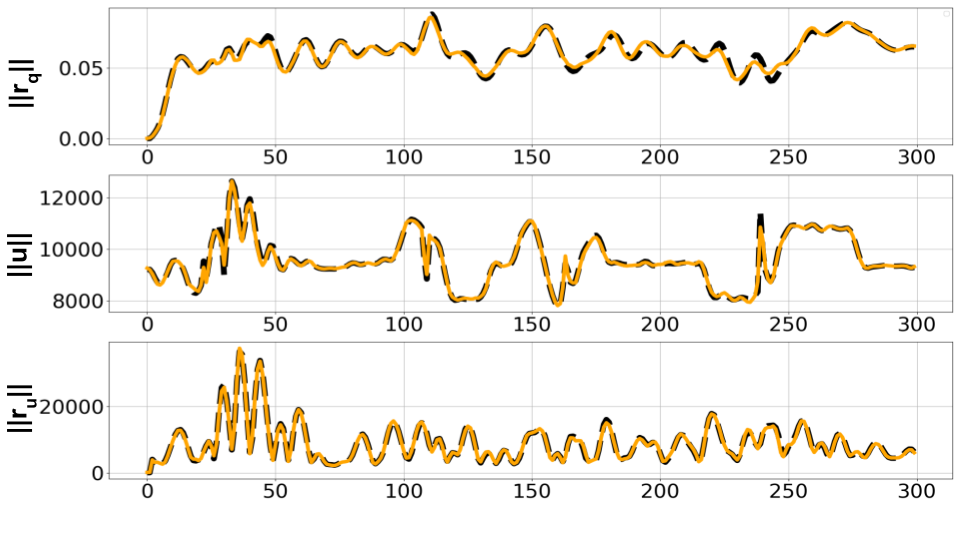
\includegraphics[width=0.8\linewidth]{figures/robust_accurate/PredNorm.png} 
    \caption{Example of GRU predictions along a trajectory (orange) against true values (back). $||\Rq||, ||\u||$ and $||\Ru||$ refer to the norm of their respective vector components. $||\Rq||$ is expressed in $m$, and control input associated values ($||\u||,||\Ru||)$ are squared propeller speeds [(rad/s)²].}%
    \label{fig: NN pred}%
\end{figure}

\begin{figure} [!t]
    \centering
    \subfloat[\centering RRT]{{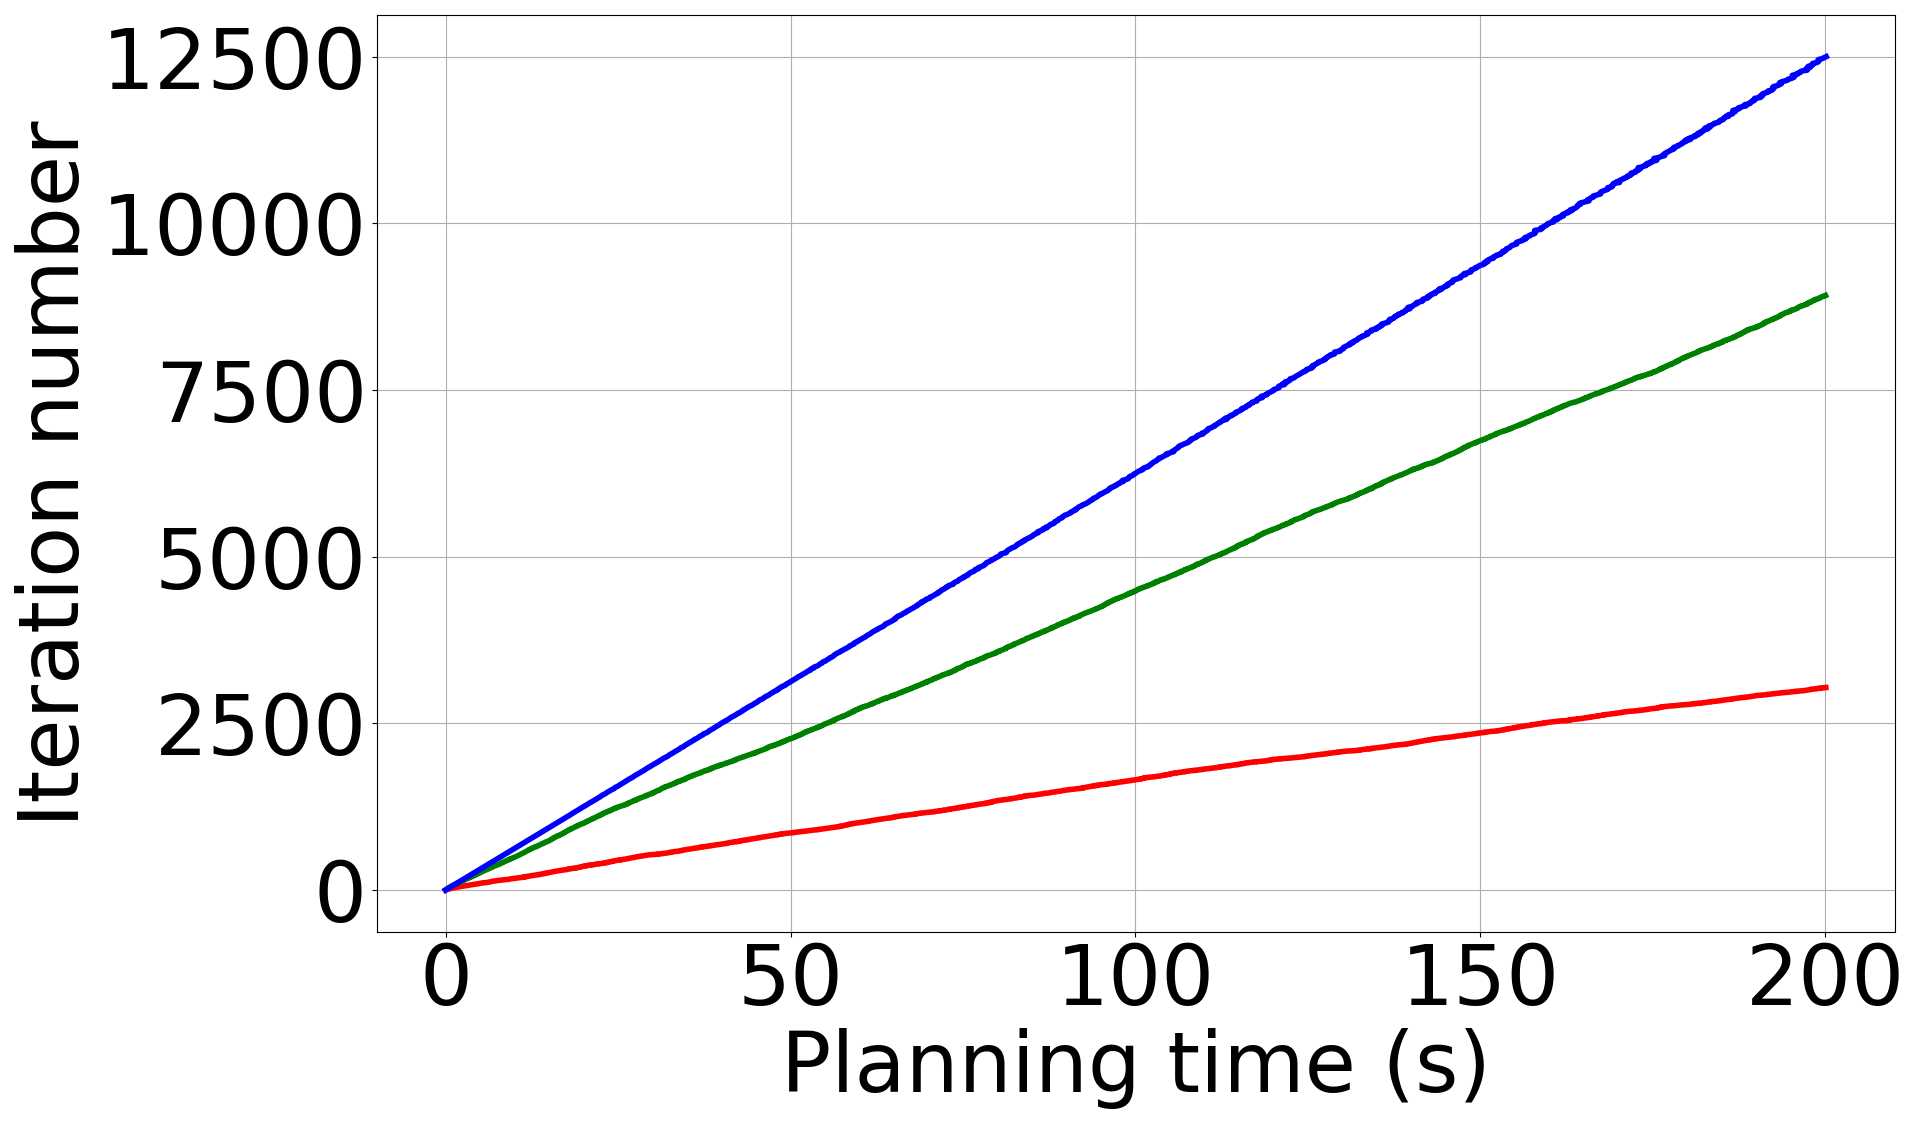
\includegraphics[width=0.4\linewidth]{figures/robust_accurate/iterations_RRT_new.png} }}%
    \subfloat[\centering RRT$^*$]{{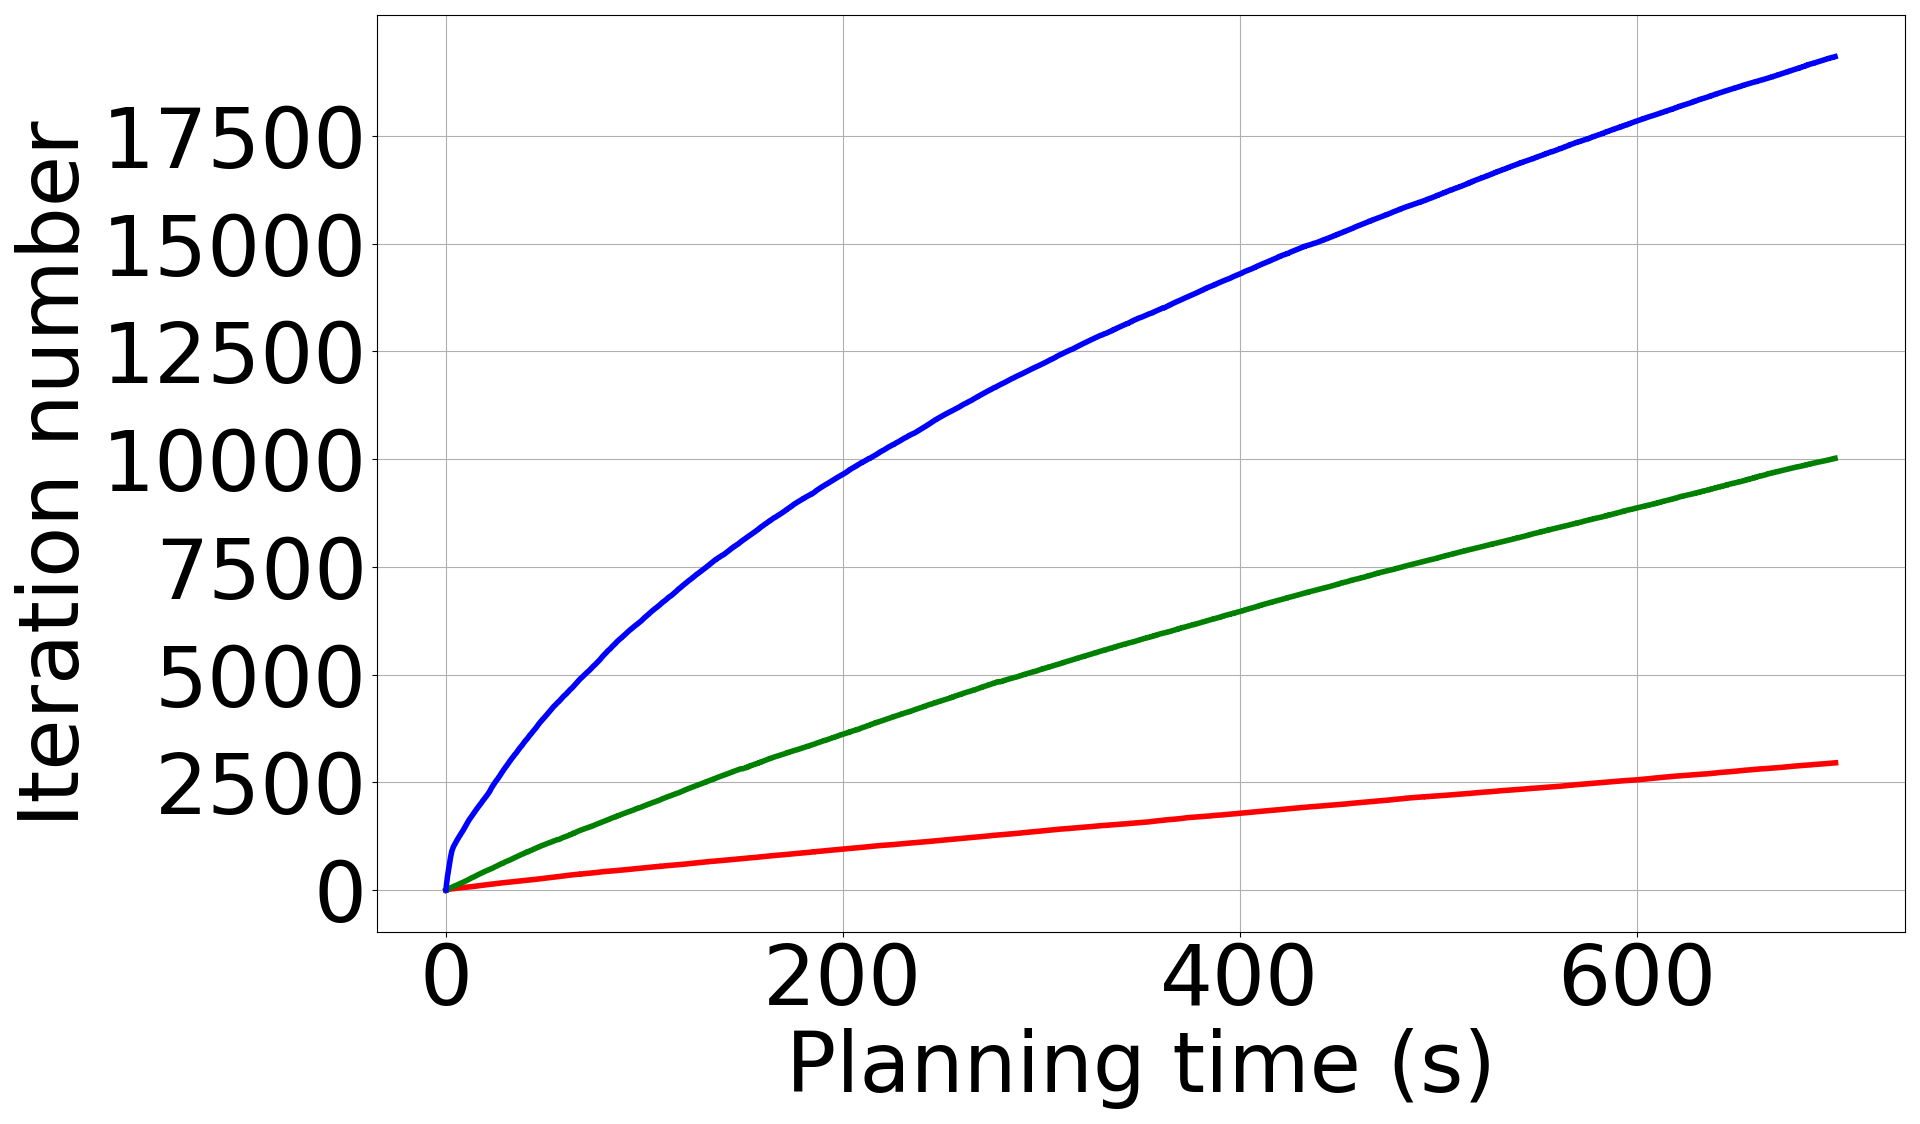
\includegraphics[width=0.4\linewidth]{figures/robust_accurate/iterations_RRTstar_new.png} }}%
    \caption{Number of (a) RRT / (b) RRT$^*$ iterations as a function of planning time in an obstacle-free environment using the standard (non-robust) RRT/RRT$^*$ implementation (blue), compared to robust versions using the GRU-based tube prediction (green) or the integration of the dynamics of $\bPi$ (red), as done in \cite{cSAMP}.}%
    \label{fig: NNTime}%
\end{figure}

\todo{Ajouter figure qui représente les pourcentage de temps passer avec le learning comparé à Sect ICRA}

Fig.~\ref{fig: NNTime} shows the significant performance improvement of using this learning-based prediction within a sampling-based tree planner for checking the robustness of the local tree expansions (see Alg.~\ref{alg:ExtensionExample}), against the previous version \cite{cSAMP} that directly integrates the $\bPi$ dynamics.  
Results provided for RRT and its RRT$^*$ near time-optimal variant compare the number of iterations of the main loop of the algorithm as a function of computing time in an obstacle-free environment, showing in both cases a significant time gain thanks to the proposed learning method compared with the method that integrates the dynamics of $\bPi$.
Note that in the case of RRT, this time gain is constant ($3$ times faster)  because the expansion benefits from the neural network only once per iteration.
In the case of RRT$^*$, the denser the tree, the more robust collision tests are required for the rewiring connection phase. 
Therefore, much more time is saved when using the learning method. 
The gain on the planning time can reach more than one order of magnitude for problems requiring a significant amount of iterations.

%%%%%%%%%%%%%%%%%%%%%%%%%%%%%%%%%%%%%%%%%%%%%%%%%%%%%%%%%%%%%%%%%%%%%%%%%%%%%%%%%%%%%%%%%%%%%%%%%%%%
\subsection{Robust planning} \label{results:RobustEval}

We first demonstrate good efficiency and robustness of the R-SARRT planner (see Sect.~\ref{sec:RSAMP}) from comparative simulation results with a standard (non-robust) RRT, a RandUp-RRT \cite{cRandUpRRT} and SARRT standing for a RRT implementation of our former framework SAMP \cite{cSAMP}.
The robust collision checking of R-SARRT and SARRT is achieved by enlarging the robot shape to account for uncertainty. 
As for RandUp-RRT, it has been implemented with 20 ``RandUP particles'' to approximate the reachable set, and no $\epsilon$-padding is used.

We also compared an asymptotically optimal version of our algorithm (R-SARRT$^*$) to 
a classic RRT$^*$ to compute near time-optimal trajectories. 
Both algorithms ran until the solution cost converged below a threshold.
Note that we cannot perform a comparison with the RandUp-RRT since there is no optimal version of the algorithm. 
The comparison is based on their planning time and success rate on the scenario depicted in Fig.\ref{fig: fig1robust}, using an Intel i9 CPU@2.6GHz and a RTX A3000 GPU for the GRU predictions.
The same geometric controller that steers the robot toward a sampled desired state $\q_d$ was used for all planners.

Table~\ref{tab:Robust window} shows comparative results averaged for each planner over 20 trajectories and 30 simulations with uncertain parameters in the range $\delta\p$ of \todo{add ref to chap model}. 
First note that RandUp-RRT, SARRT and R-SARRT have a much stronger robustness than standard non-robust RRT. 
R-SARRT has a success rate of 100\% compared to 99,2\% for RanUp-RRT. 
Indeed, as mentioned in \cite{cRandUpRRT, cRandUP}, the computation of a conservative reachable set requires some additional padding step, which is set to zero in our experiment\footnote{The padding value is a user parameter that is difficult to find. Choosing the wrong padding value can result in set estimations that are too conservative. We chose zero as in some experiments of \cite{cRandUpRRT}.}. 
Also note the higher efficiency of R-SARRT which only uses one prediction per iteration whereas RandUp-RRT needs to perform a propagation per particle, yielding to a longer planning time. 
As for SARRT, it does not build a robust tree like R-SARRT. Instead, it only robustly checks the final solution, causing frequent disconnections and re-connections of non-robust nodes, which results in a higher planning time.
RRT, which does not account for robustness, remains faster but with a significantly lower success rate. 
Similar results are observed on the optimal versions. 
An example of trajectories planned by RRT$^*$ and a robust version R-SARRT$^*$ optimizing the trajectory duration, and their associated simulations, is illustrated in Fig.\ref{fig: simu window}.
It shows the effective robustness of the proposed algorithm as illustrated by the higher success rate indicated in Table \ref{tab:Robust window}.

We also experimentally demonstrate the window scenario on a real quadrotor.
Uncertainties are added to the system by randomly attaching a mass of up to 80g (not known by the controller) to the drone as depicted in Fig.\ref{fig: drone_mass}.

\begin{table*}[t]
    \centering
    \begin{tabular}{l|llll|ll|}
    \cline{2-7}
    & \multicolumn{4}{c||}{Basic Planners} & \multicolumn{2}{c|}{Asymptotically Optimal Planners} \\ \cline{2-7} 
        & \multicolumn{1}{c|}{RRT} & \multicolumn{1}{c|}{RandUp-RRT} & \multicolumn{1}{c|}{SARRT} & \multicolumn{1}{c||}{R-SARRT} & \multicolumn{1}{c|}{RRT$^{*}$} & \multicolumn{1}{c|}{R-SARRT$^*$} \\ \hline
    \multicolumn{1}{|c|}{Success (\%)} & \multicolumn{1}{c|}{61.8}   & \multicolumn{1}{c|}{99.2} & \multicolumn{1}{c|}{\textbf{100.0}}  &   \multicolumn{1}{c||}{\textbf{100.0}}   & \multicolumn{1}{c|}{56.5}   &  \multicolumn{1}{c|}{\textbf{100.0}}   \\ \hline
    \multicolumn{1}{|c|}{Plan time (s)} & \multicolumn{1}{c|}{\textbf{7.1} $\pm$ 7.6}   & \multicolumn{1}{c|}{45.6 $\pm$ 33.4} & \multicolumn{1}{c|}{57.8 $\pm$ 49.1}  &   \multicolumn{1}{c||}{ 22.3 $\pm$ 15.8}  & \multicolumn{1}{c|}{\textbf{308.7} $\pm$ 235.7}   &  \multicolumn{1}{c|}{584.3 $\pm$ 394.7}    \\ \hline
    \end{tabular}
    \caption{
    \label{tab:Robust window}
    Average planning time and success rate (no crash) of the simulated motions planned by RRT, RandUP-RRT, our former planner SARRT and our R-SARRT, as well as RRT$^{*}$ and our  R-SARRT$^{*}$ variants optimizing time, over 20 plans and 30 simulations per plan.}
\end{table*}

\begin{figure} [h]
    \centering
    \subfloat[\centering RRT$^*$]{{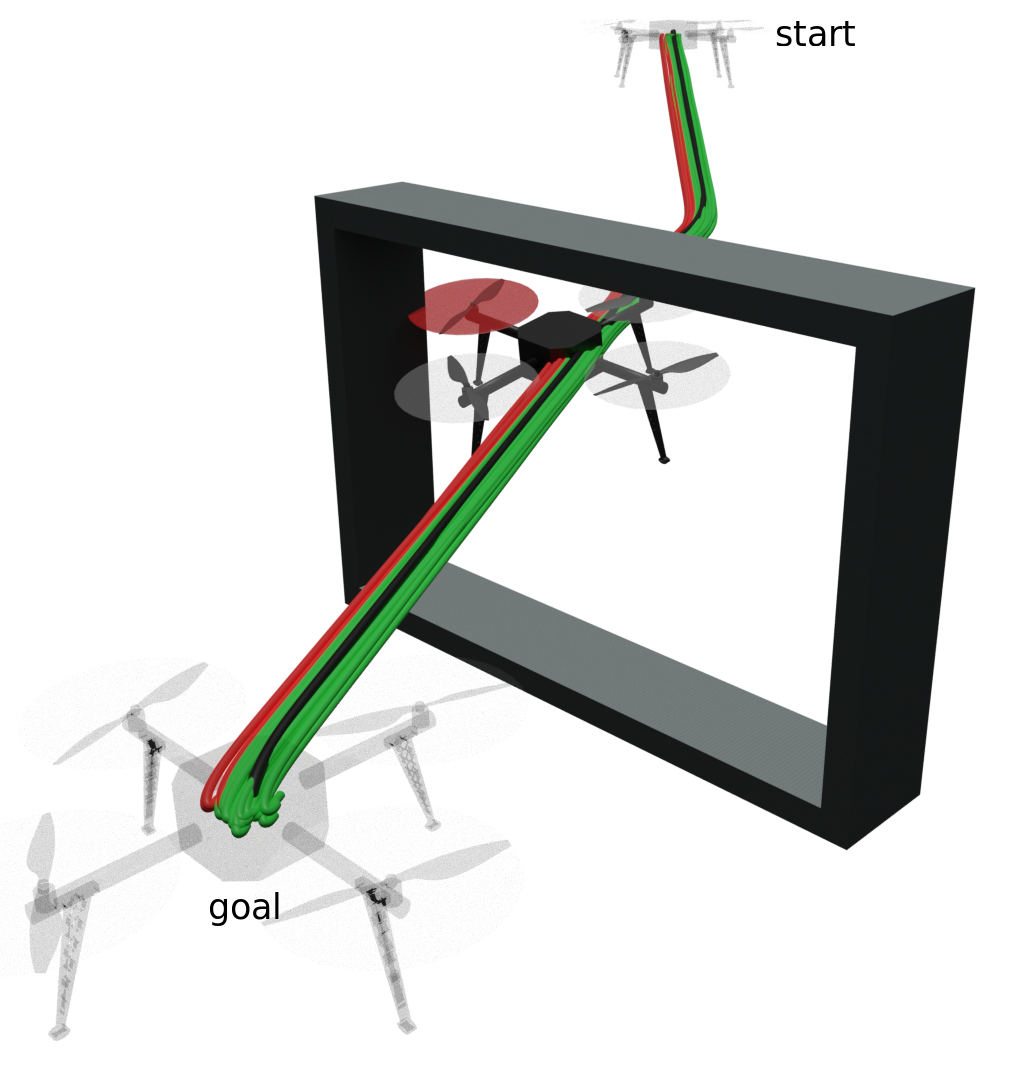
\includegraphics[width=0.4\linewidth]{figures/robust_accurate/simu_RRTstar_notube.png} }}%
    \subfloat[\centering R-SARRT$^*$]{{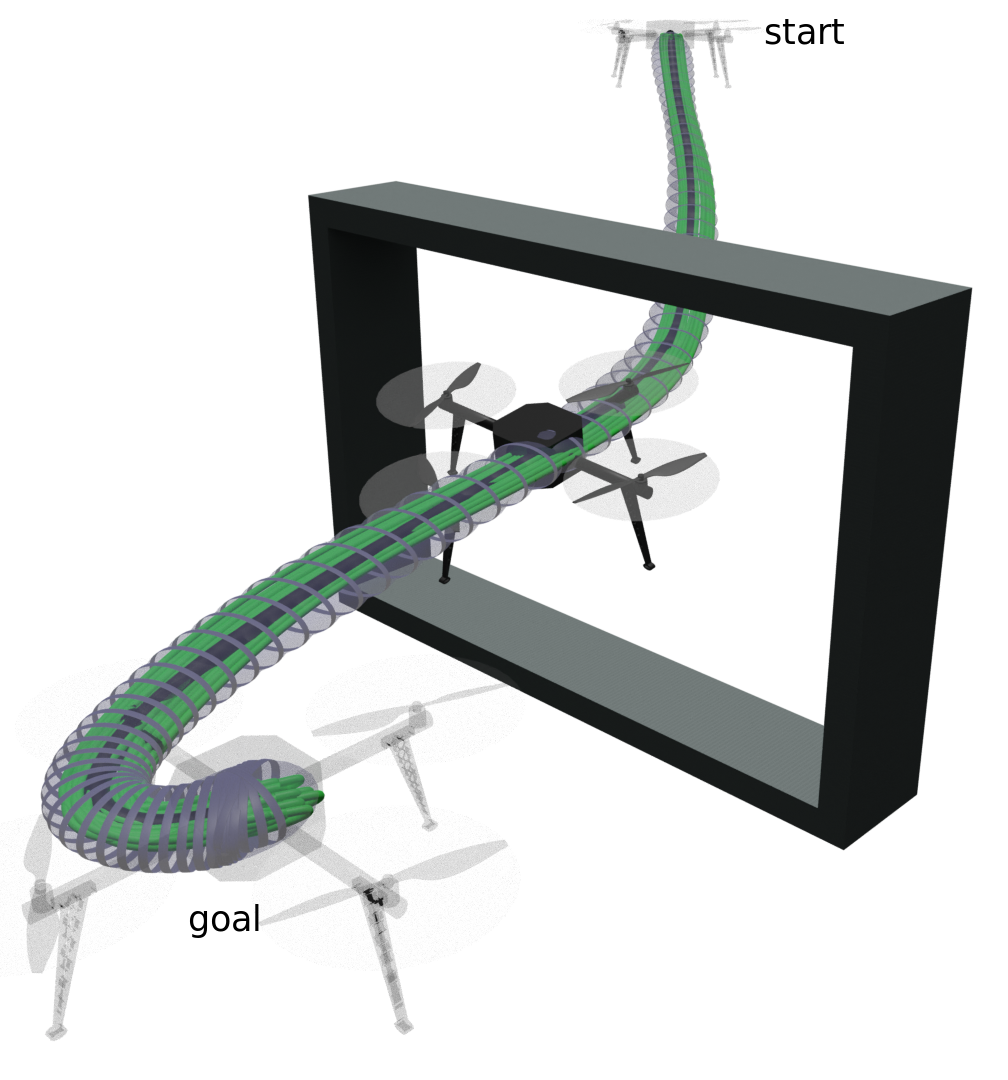
\includegraphics[width=0.4\linewidth]{figures/robust_accurate/simu_SARRTstar.png} }}%
    \caption{Planned trajectory (black) produced by a (a) RRT$^*$ and our (b) R-SARRT$^*$. 
    Simulated trajectories under uncertainty are displayed in green in the case of success, and in red in the case of a crash.}%
    \label{fig: simu window}%
\end{figure}

\begin{figure} [h]
    \centering
    
    \subfloat[\centering ]{{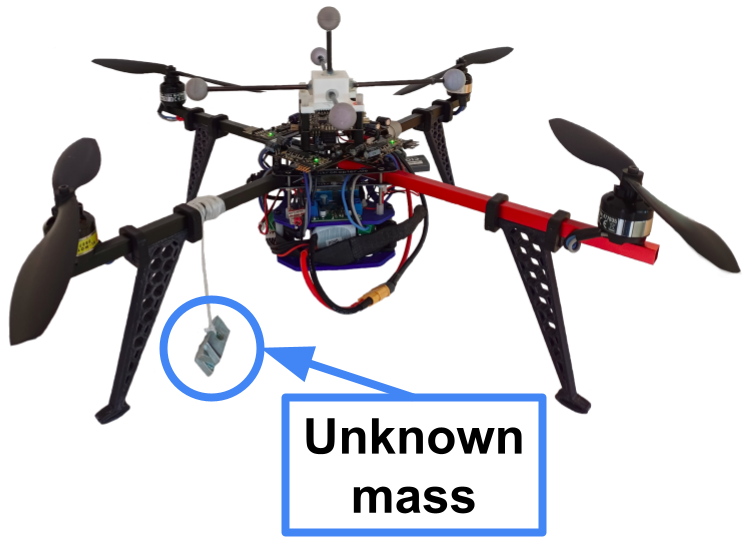
\includegraphics[width=0.42\linewidth]{figures/robust_accurate/drone_window.png} }\label{fig: drone_mass}}%
    \subfloat[\centering ]{{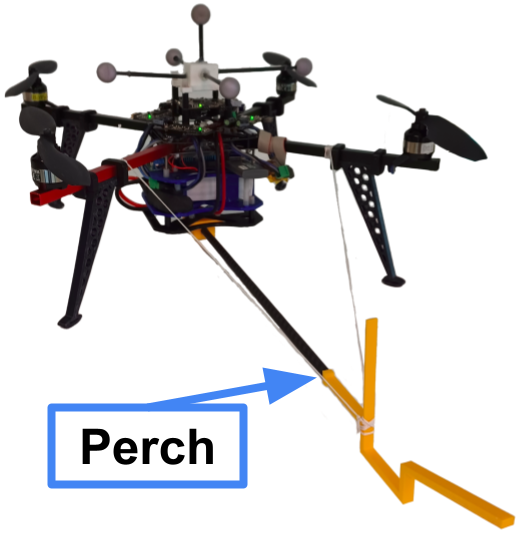
\includegraphics[width=0.3\linewidth]{figures/robust_accurate/drone_perch.png}} \label{fig: drone_perch}}%
    
    \caption{Quadrotor setups for the two scenarios considered for the experimental validation. (a) a drone equipped with a random mass to perform a robust navigation through a window (b) a drone equipped with a perch to catch the rings.}%
    \label{fig: exp setup}%
\end{figure}

\begin{figure} [h]
    \centering
    \subfloat[\centering RRT$^{*}$]{{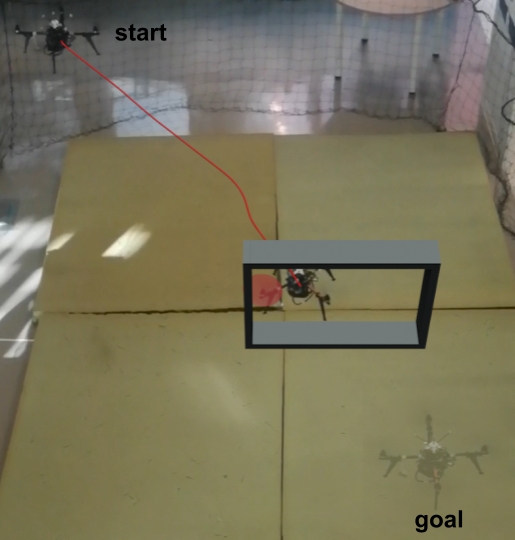
\includegraphics[width=0.4\linewidth]{figures/robust_accurate/exp_RRTstar.png} }}%
    \subfloat[\centering R-SARRT$^*$]{{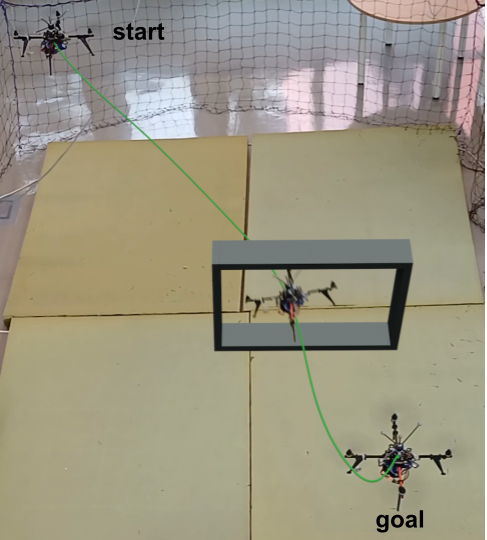
\includegraphics[width=0.378\linewidth]{figures/robust_accurate/exp_SARRTstar.png} }}%
    \caption{Experimental execution by a quadrotor with uncertainty of trajectories planned by  RRT$^*$ (a) and  R-SARRT$^*$ (b). Both trajectories are executed with the same uncertainty and a virtual collision is found in the RRT$^*$ case while the R-SARRT$^*$ execution is robust.}%
    \label{fig: exp window}%
\end{figure}

In this experiment, a non-robust trajectory planned by RRT$^*$ and a robust one planned by R-SARRT$^*$ were executed ten times, using the same masses and attachment points between the two algorithms.
All trajectories were planned offline on a remote computer. To make the robot execute them, the geometric controller~\cite{cLee} ran online on the quadrotor's onboard computer, tracking the trajectories provided as input. The robot state was measured using a motion capture system with millimeter accuracy, ensuring that the only source of uncertainty was the attached unknown mass.
Fig.\ref{fig: exp window} illustrates the experimental execution of a non-robust RRT$^*$ trajectory and a robust R-SARRT$^*$ trajectory. 
The figure shows the recorded executions within a virtual environment to detect virtual collisions, thus mitigating the risk of real crashes and damages to the robot.
The experimental results confirm the simulation observations, providing an overall success rate of 100\% in the case of the robust trajectory computed with R-SARRT$^*$, against 40\% for the classic RRT$^*$.

%%%%%%%%%%%%%%%%%%%%%%%%%%%%%%%%%%%%%%%%%%%%%%%%%%%%%%%%%%%%%%%%%%%%%%%%%%%%%%%%%%%%%%%%%%%%%%%%%%%%
\subsection{Accuracy optimization} \label{results:AccEval}

\begin{figure} [t]
    \centering
    {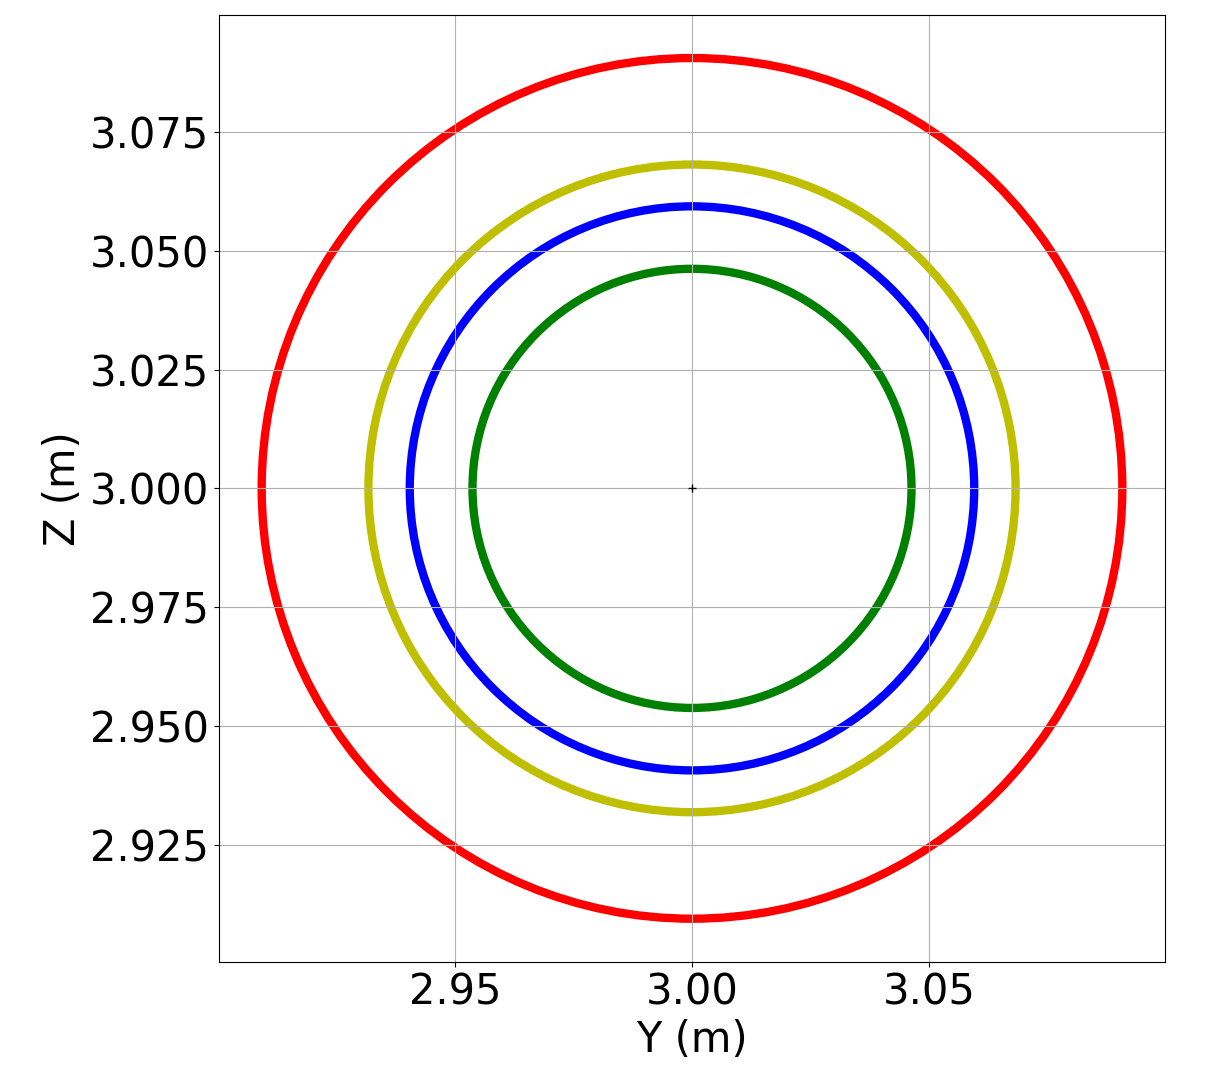
\includegraphics[width=0.5\linewidth]{figures/robust_accurate/accuracy_opti.png} }%
    \caption{Example of uncertainty ellipsoid without optimization (red), with local trajectory optimization (yellow), with gains optimization (blue), and with local trajectory and gains optimization at the same time (green).}%
    \label{fig: Acc opti}%
\end{figure}

\begin{figure} [t]
  \begin{subfigure}{0.63\linewidth}
    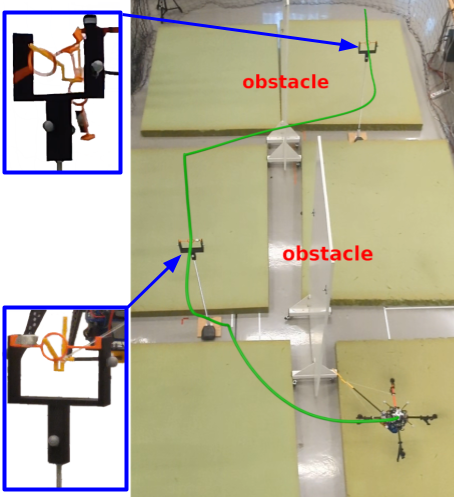
\includegraphics[width=\linewidth]{figures/robust_accurate/ring_opti_v1.png}
  \end{subfigure}\hfill
  \begin{subfigure}{0.37\linewidth}
      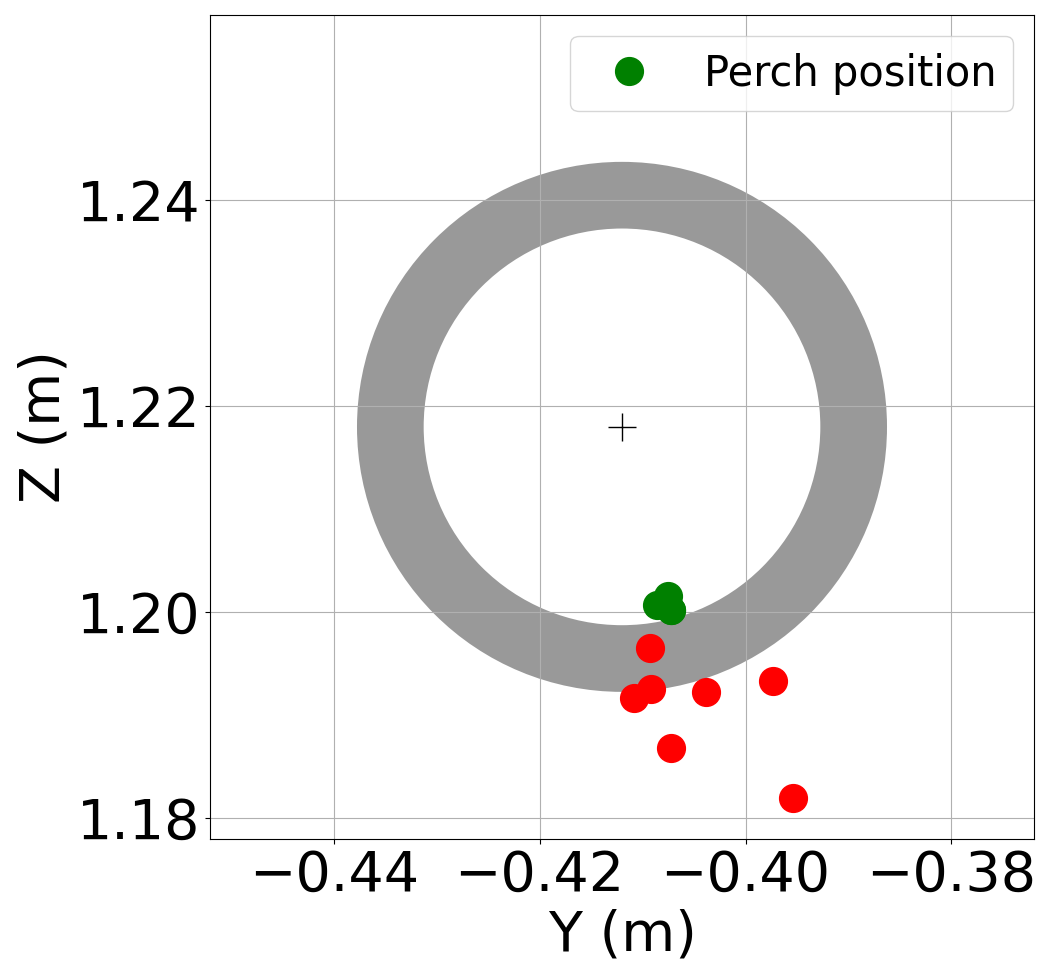
\includegraphics[width=\linewidth]{figures/robust_accurate/Exp_ring_no_opti_full_zoom.png}
      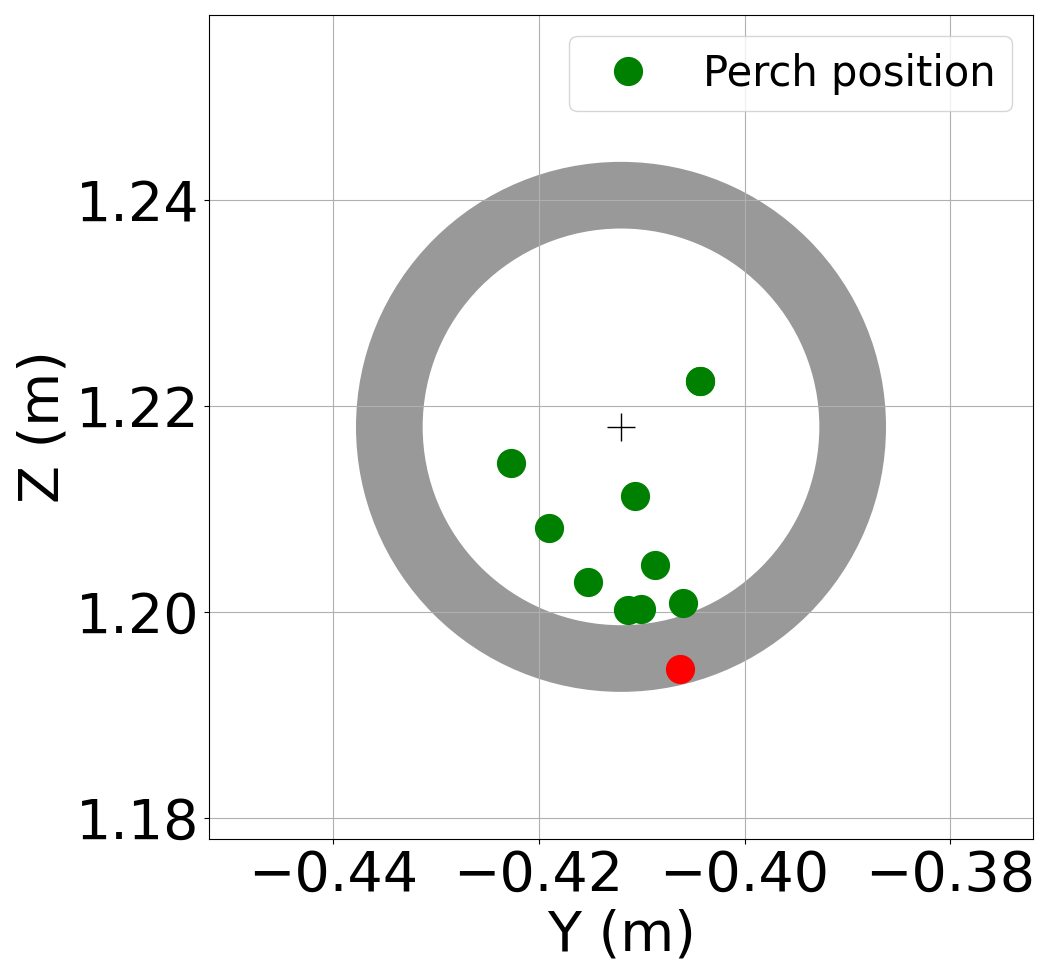
\includegraphics[width=\linewidth]{figures/robust_accurate/Exp_ring_opti_full_zoom.png}
    \end{subfigure}\hfill
    
  \caption{Experimental validation of the ``ring catching'' scenario with a perch-equipped drone (left) with the position of the perch end-effector at the second ring location over 10 trajectories non accuracy optimized (top right) and accuracy optimized (bottom right).}
  \label{fig: exp ring}
\end{figure}

We implemented the A-Optim method of Sect.\ref{sec:AOptim} by using a robust version of the random shortcut algorithm \cite{cShortcut} and \eqref{eq: cost} as cost function to be optimized, where the radii of interest are the ones along the $\boldsymbol{x}$, $\boldsymbol{\rho}$ and $\boldsymbol{\omega}$ components of $\boldsymbol{q}$.
At each iteration of this method, a shortcut is attempted between two states of the input trajectory that are randomly sampled together with the controller gain values, sampled between 50\% and 150\% of their nominal values.
Fig.\ref{fig: Acc opti} motivates why we optimized both the trajectory and the controller gains at the same time in the A-Optim function in order to minimize uncertainty for a given point, as mentioned in Sec.\ref{sec:RASAMP}. In fact, these results corroborate the findings of \cite{AliIROS}, but this time by employing a sampling-based motion planner that considers obstacles in the environment.

We evaluated our complete framework with the accuracy optimization in a scenario that involves the in-flight retrieval of two 2cm radius rings in a cluttered environment using a drone equipped with a perch (see Fig.\ref{fig: drone_perch}) in a (near) time optimal way.
The experimental setup is shown in Fig.\ref{fig: exp ring}.
When the first ring is caught it becomes part of the drone and modifies the overall mass/inertia and center of mass of the system in an unmodeled way. 
A success is characterized by the recovery of both rings, otherwise we consider the execution as a failure.

We executed 10 trajectories using a vanilla (non-robust) RRT$^*$ planner and the RA-SARRT$^*$ algorithm, both of which optimize the trajectory time.
The RRT$^*$ does not use the A-Optim method to optimize accuracy while the RA-SARRT$^*$ does, in addition to guaranteeing the robustness.
The offline optimization in A-Optim aimed at minimizing the uncertainty at the location of the two rings.
Fig.~\ref{fig: exp ring} shows the perch end-effector position at the second ring location in the non-optimized case and in the optimized one. 
In the latter case, the perch tip is closer to the reference point in the middle of the ring than in the former case. This translates into a higher success rate of nine out of ten attempts to catch the ring with the optimized approach, against only three times out of ten for the non-optimized case.
However, given the chosen system and controller parameters, there is no guarantee that the computed tube will be enclosed in within the ring.
This explains why we still encounter one failure in the optimized case.
Overall, the experimental results show a success rate of 90\% for RA-SARRT$^*$ against only 30\% for RRT$^*$.

\section{Experimental validation} \label{sec:Experimental}

%%%%%%%%%%%%%%%%%%%%%%%%%%%%%%%%%%%%%%%%%%%%%%%%%%%%%%%%%%%%%%%%%%%%%%%%%%%%%%%%%%%%%%%%%%%%%%%%%%%%
\section{Conclusion} \label{sec:Conclusion}

We have presented a motion planner able to generate trajectories that are both robust and accurate in the presence of model uncertainties for a variety of robot/controller pair. The proposed planner leverages a GRU-based learning approach that quickly and accurately estimates the control inputs and the sensitivity-based uncertainty tubes of the state and of the inputs. 
The results on a quadrotor robot confirm the efficiency of the proposed learning method and highlight the benefit of its integration within a motion planner, resulting in a significant reduction of the planning times. 
Moreover, we showed that our framework is able to locally optimize the planned trajectory in order to minimize the size of the uncertainty tubes of the state at some desired locations, allowing the system to accurately perform a precision task. An experimental demonstration involving a quadrotor UAV in a ring-catching task allowed to validate the approach in real conditions. Future works will focus on considering uncertainties not only in the dynamic model, by extending the computation of the tubes for state estimation uncertainties. 
Furthermore, we aim to expand the capabilities of the neural network to learn the optimal controller gains.


\todomarker{}
% \cleardoublepage
% \newpage 
% \ % The empty page
% \newpage
\chapter{Conclusion}
\markboth{Conclusion}{}% To set left/right header

\glsresetall

In this thesis, 

\paragraph{Future Works} Several xxxx 

% \cleardoublepage
% \newpage 
% \ % The empty page
% \newpage
\appendix
\chapter{Robust feasibility checking}\label{chap:appendixA}

% \begin{figure} [t]
%     \centering
%     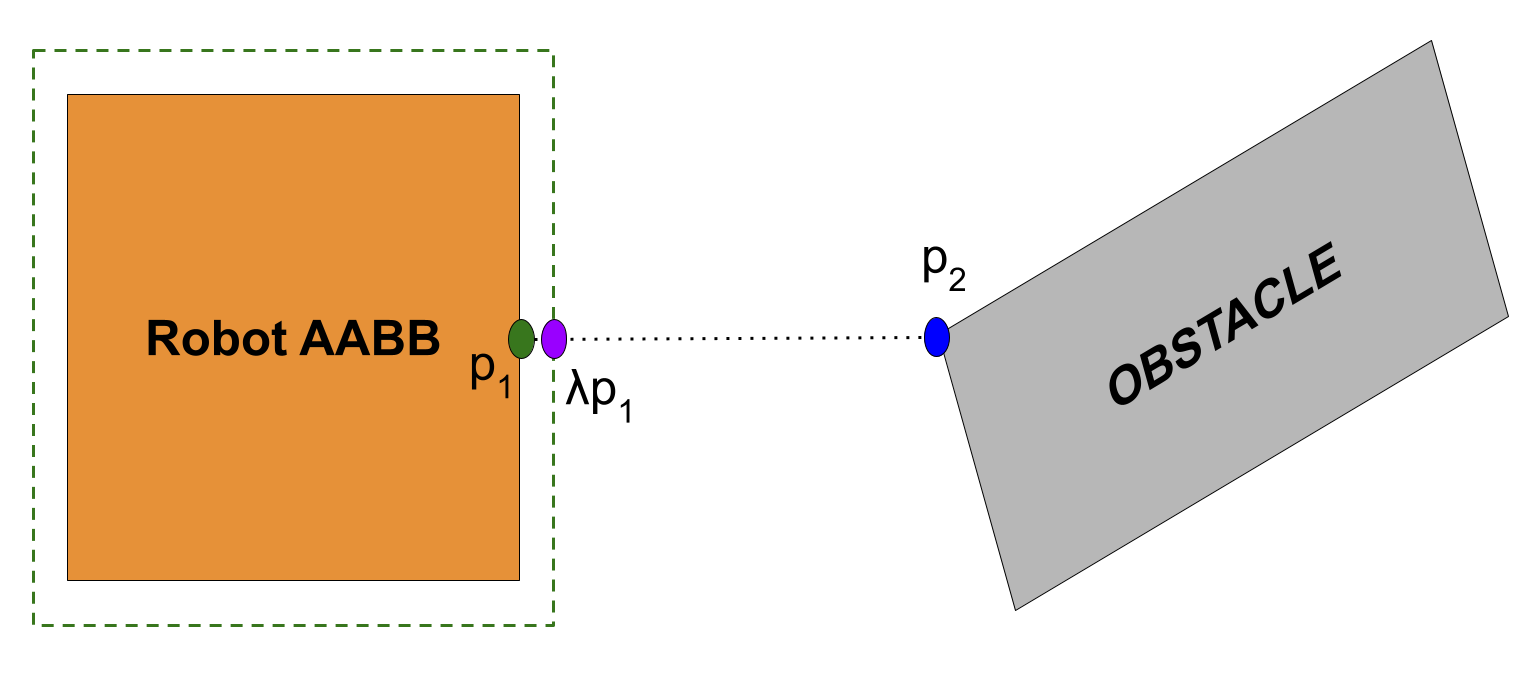
\includegraphics[width=0.8\linewidth]{figures/appendix/CCellipse.png}
%     \caption{Collision checking given a uniform scaling of the robot AABB.}
%     \label{fig:appendix_A}
% \end{figure}

% Given a current robot AABB, this proof aims to show that the closest point on the robot to an obstacle remains the closest point after uniform scaling, and that the closest point of the obstacle to the robot also remains unchanged (see Figure~\ref{fig:appendix_A}).

% Let $A$ and $B$ be two convex sets. 
% This assumption holds for the collision test presented in Section~\ref{sec:robust_CC} as the robot AABB is a convex shape, and the environment is decomposed into convex shapes.
% Let \( p_1 \in A \) such that \( p_1 = \arg \min_{a \in A} \|a - b\| \, \forall b \in B \), and \( p_2 \in B \) such that \( p_2 = \arg \min_{b \in B} \|a - b\| \, \forall a \in A \).
% Also let $\lambda A, \lambda \geq 1$ be a uniform scaling of $A$.

% One want to show that:
% \begin{enumerate}
%     \item The projection of $p_1$ due to the scaling remains the closest point to the obstacle.
%     \item $p_2$ remains the closest point to the projection of $p_1$. 
% \end{enumerate}
% \[
%     \left\{
%     \begin{aligned}
%         \lambda p_1 &= \argmin_{a \in A} \|\lambda a - b\| \, \forall b \in B \\
%         p_2 &= \argmin_{b \in B} \|\lambda p_1 - b\|
%     \end{aligned}
%     \right.
% \]

% \paragraph{1.}
% Let \( a \in A \) and \( b \in B \).
% One can express the following relationship:
% \[
% \|\lambda a - b\| = \lambda \left\|a - \frac{b}{\lambda}\right\|,
% \]
% where \(\frac{b}{\lambda} \in B\) because \(B\) is convex. 
% Therefore, one gets:
% \[
% \arg \min_{a \in A} \left\|a - \frac{b}{\lambda}\right\| = \arg \min_{a \in A} \|a - b\| = p_1,
% \]
% which implies:
% \[
% \arg \min_{a \in A} \|\lambda a - b\| = \lambda p_1.
% \]

% \paragraph{2.}
% Let \( b \in B \), \( b \neq p_2 \) such that:

% \[
% \|\lambda p_1 - b\|^2 = \|\lambda p_1 - p_2\|^2 + \|p_2 - b\|^2,
% \]
% and since \( p_2 \neq b \), one gets \( \|p_2 - b\|^2 > 0 \). 
% Therefore, \( \|\lambda p_1 - b\| > \|\lambda p_1 - p_2\| \), which implies \( \arg \min_{b \in B} \|\lambda p_1 - b\| = p_2 \).

Sampling-based algorithms generate global trajectories by combining multiple continuous local trajectories.
During the process, each of these local trajectories are subject to collision checks to determine their feasibility.
However, in this thesis, the collision check is extended to include a more general feasibility test, which also accounts for the control input space. 
This extension ensures that the generated trajectories are not only free from obstacles but also prevent control inputs from reaching saturation. 
Additionally, it accounts for uncertainty in both the state and control input spaces, further enhancing the robustness of the trajectories.
The following appendix describes how these extended feasibility check is performed to ensure the robustness of each local trajectory in this context.
It is important to note that these test is not continuous; rather, it is performed along a discrete representation of the local trajectories, sampled at the controller's operating frequency.

\paragraph{Robust collision checking}

In this thesis, collision detection is performed using the widely used C implementation of PyBullet~\cite{cBullet}, which operates as follows: 
\begin{enumerate}
    \item It starts with a broad-phase collision detection using \myglsentry{AABBs} to quickly eliminate pairs of objects that are too far apart to collide, allowing the more computationally intensive collision checks to focus only on pairs that are potentially close to each other.
    \item Then, it performs a narrow-phase collision detection that, after potential collision pairs are identified, checks for each pair. 
    For each identified potential collision pair, this phase uses a more precise robot representation (as defined by the user) and specialized collision algorithms to detect actual intersections and determine contact points, normals, and penetration depths.
\end{enumerate}

Extending this procedure to account for robot state uncertainty aims to verify that the resulting extended bounding volume, which the robot may occupy due to the uncertainty, is clear of obstacles.
In this work, such bounding volume is computed by considering only the uncertainty in the position subspace for simplicity (i.e., the $\{x,y,z\}$-subspace for the quadrotor or the $\{x,y\}$-subspace for the differential drive robot).

This work employ a robust collision check generic to all free flying robots that operates as follows:
\begin{enumerate}
    \item As mentioned above, the first phase performs a broad collision detection considering the current robot AABB. 
    Therefore, in the robust collision detection of this work, this phase involves creating an extended AABB by scaling the current robot AABB in all directions according to their respective uncertainty radii as shown in Figure~\ref{fig:CCmethods}. 
    \item The narrow phase approach leverage a fine robot representation.
    However, generating the accurate extended collision mesh that incorporates uncertainty, required for the second phase, is challenging, as it involves deforming all the vertices of the robot mesh.
    To address this, this work approximate the extended collision mesh by sampling on the surface of the uncertainty ellipsoid bounding box defined by the uncertainty tube radii (see Figure~\ref{fig:CCmethods}). 
    While this method accurately approximates the true extended collision shape, it requires multiple calls to the collision-checking function for each robot state tested.
\end{enumerate}

\begin{figure}[htp]
    \centering
    % Row 1
    \begin{subfigure}{0.4\textwidth}
        \centering
        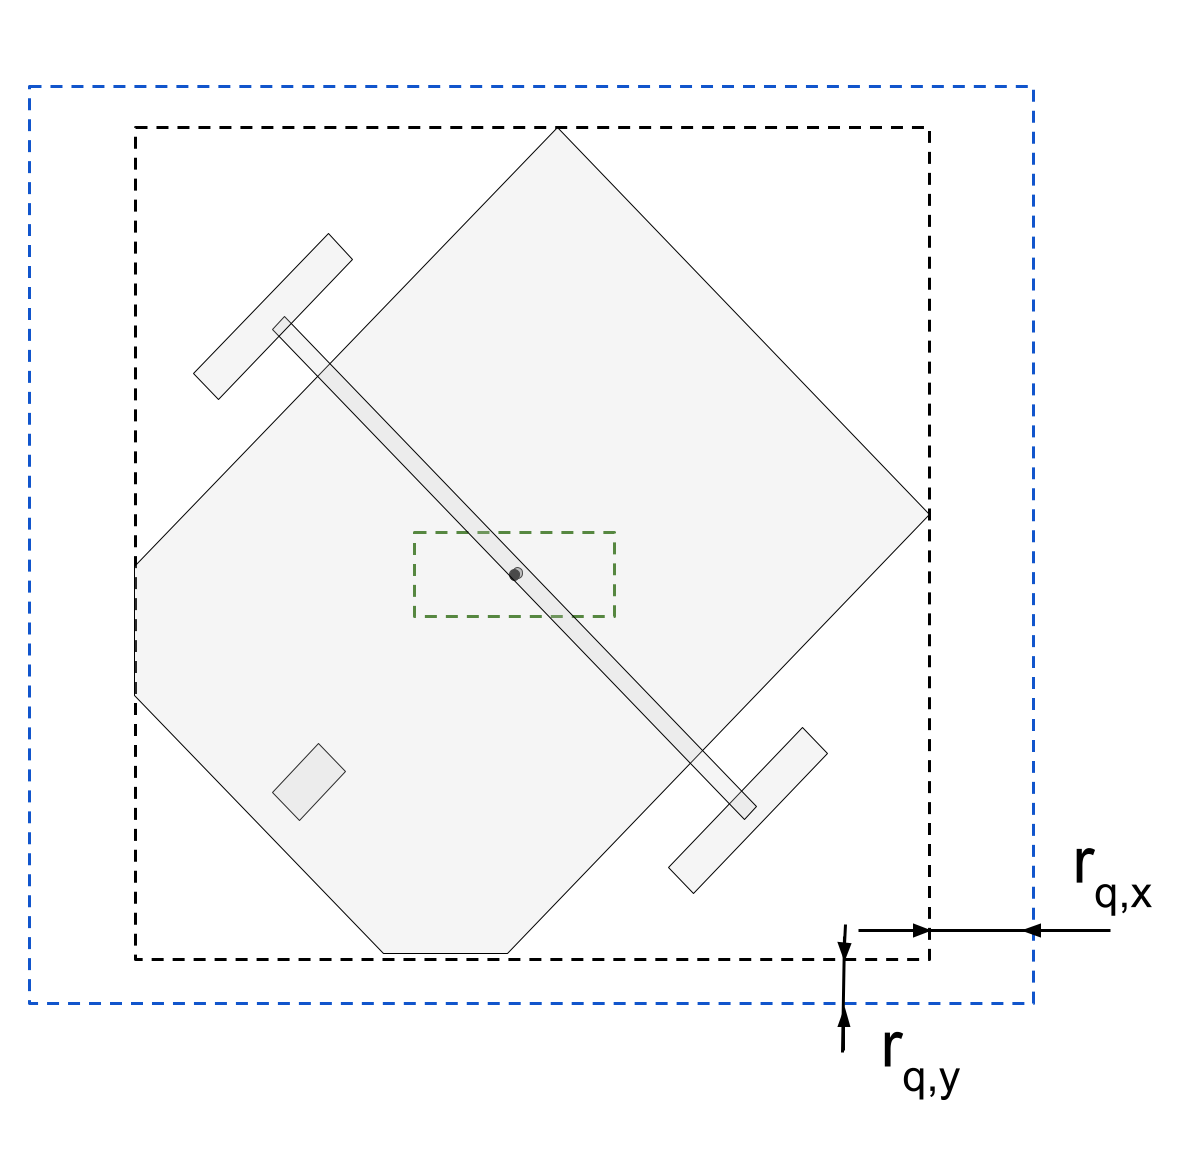
\includegraphics[width=\linewidth]{figures/samp/CC2.png}
        \caption{}
        \label{fig:CC1}
    \end{subfigure}
    % \hfill
    \begin{subfigure}{0.4\textwidth}
        \centering
        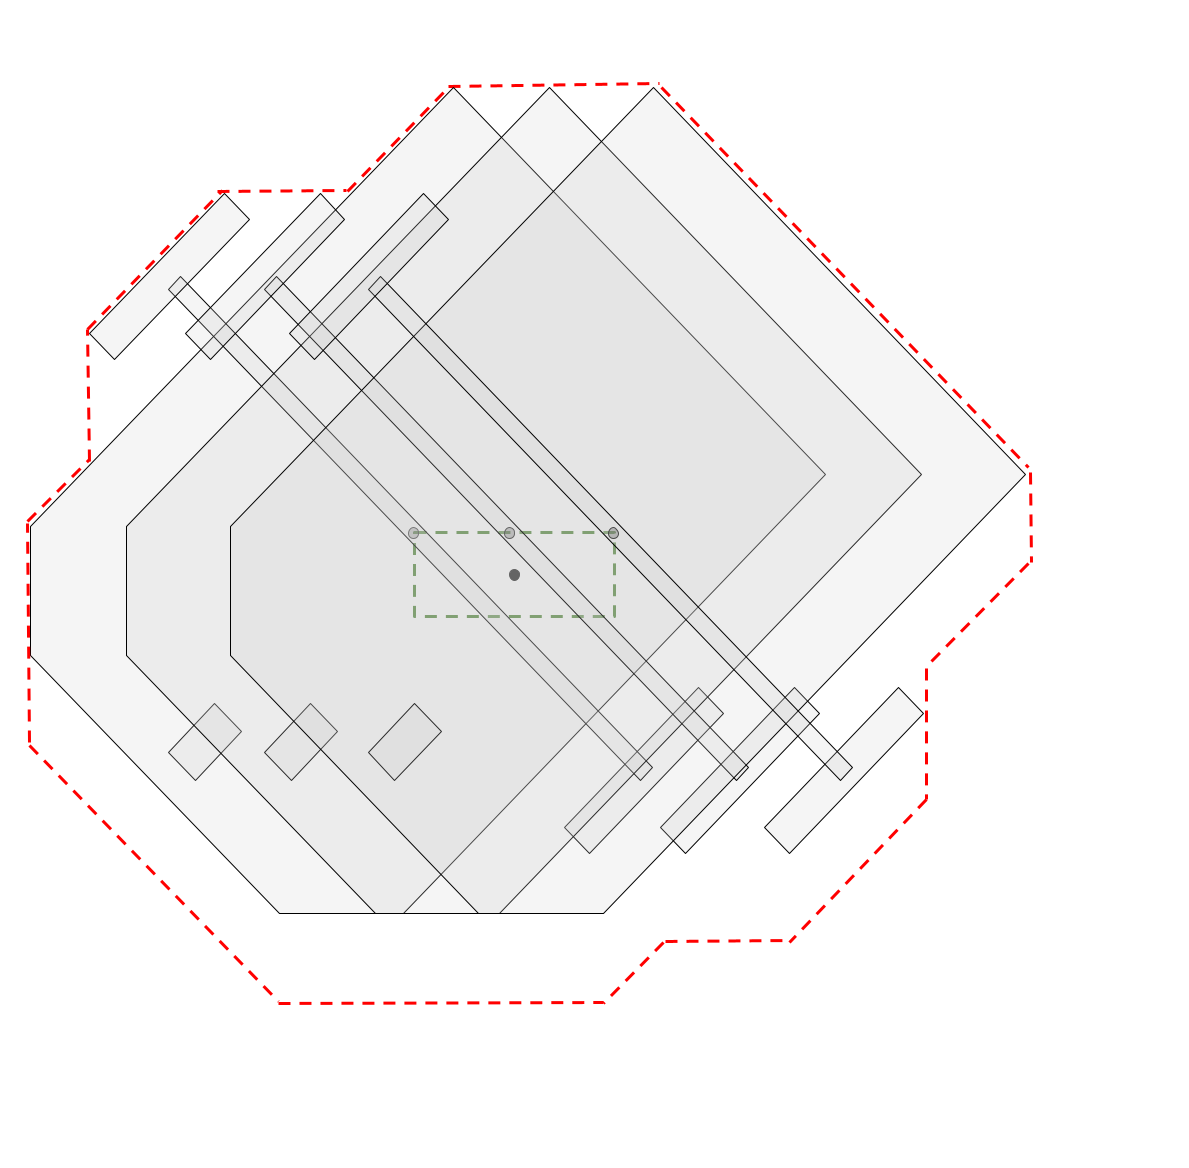
\includegraphics[width=\linewidth]{figures/samp/CC3.png}
        \caption{}
        \label{fig:CC2}
    \end{subfigure}
    
    % Row 2
    \begin{subfigure}{0.4\textwidth}
        \centering
        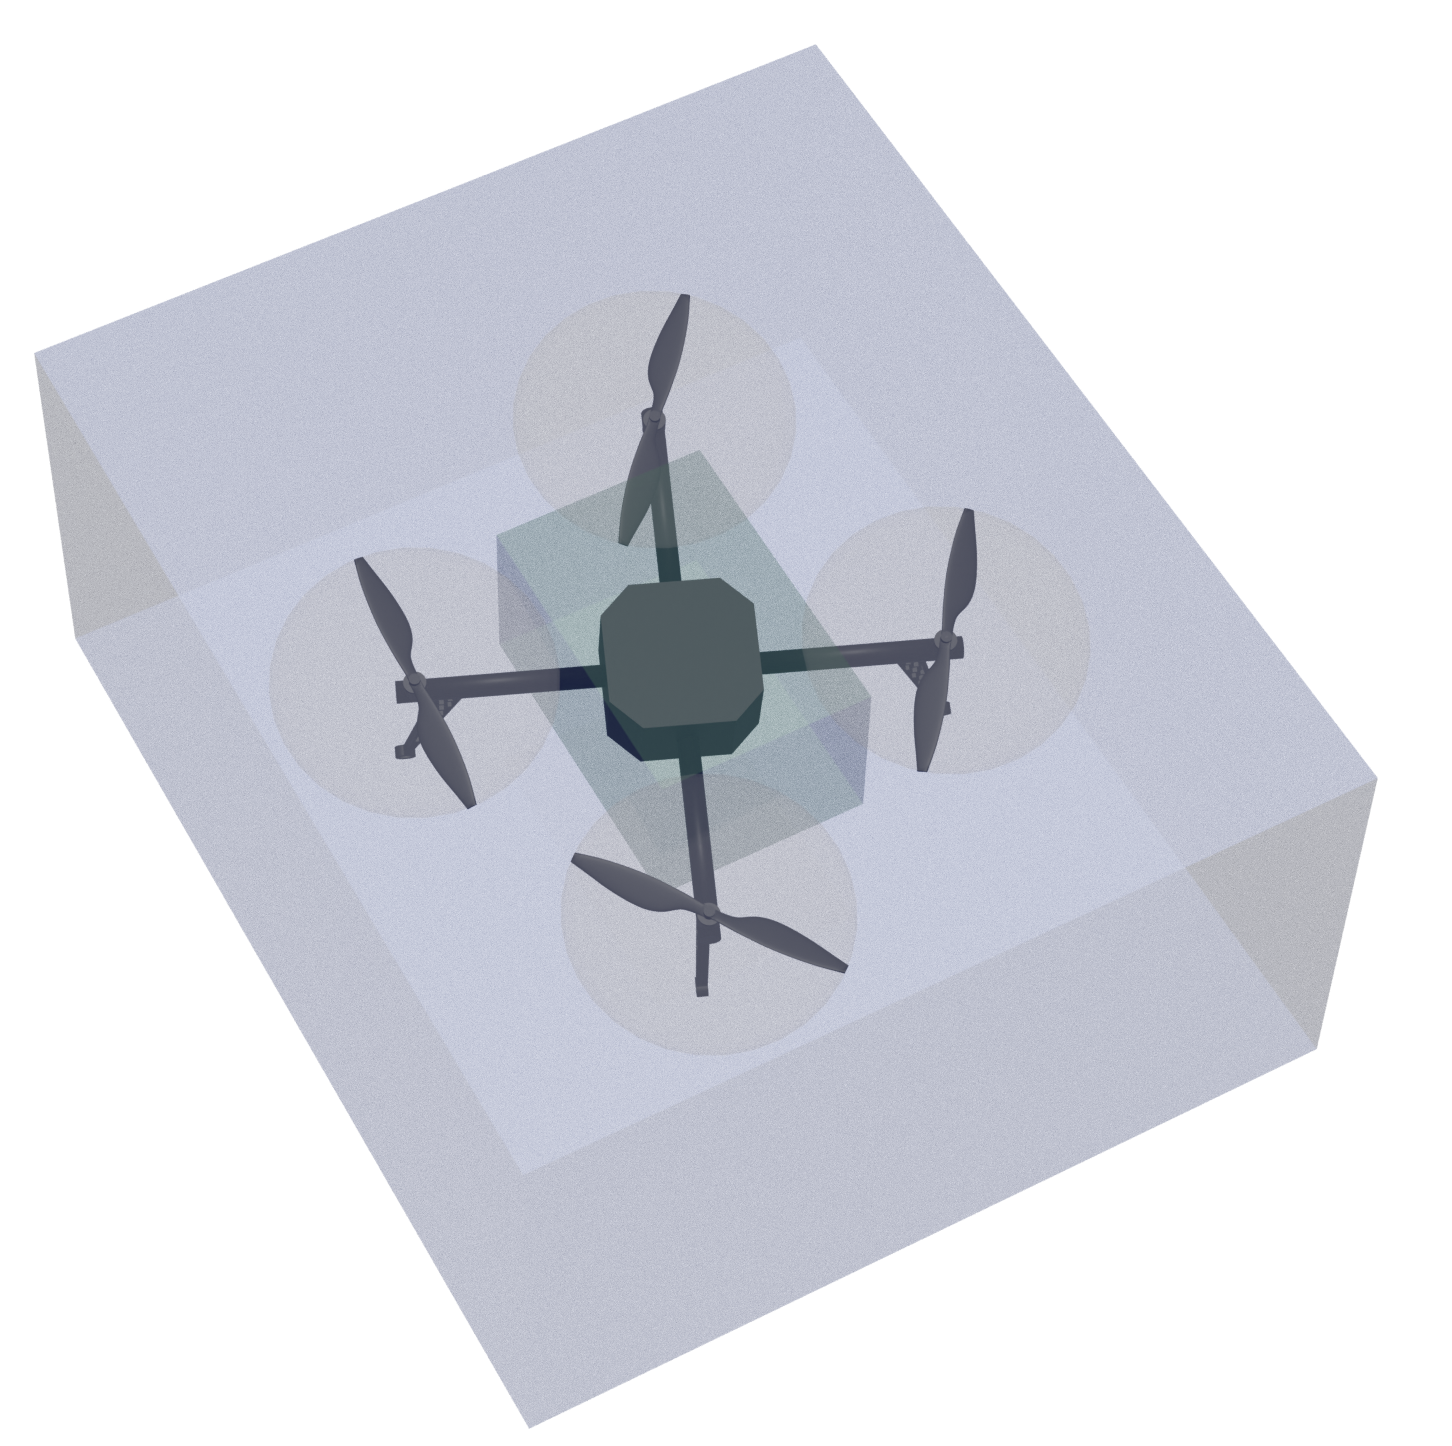
\includegraphics[width=\linewidth]{figures/appendix/CCdrone1.png}
        \caption{}
        \vspace{-0.3cm}
        \label{fig:CC3}
    \end{subfigure}
    % \hfill
    \begin{subfigure}{0.4\textwidth}
        \centering
        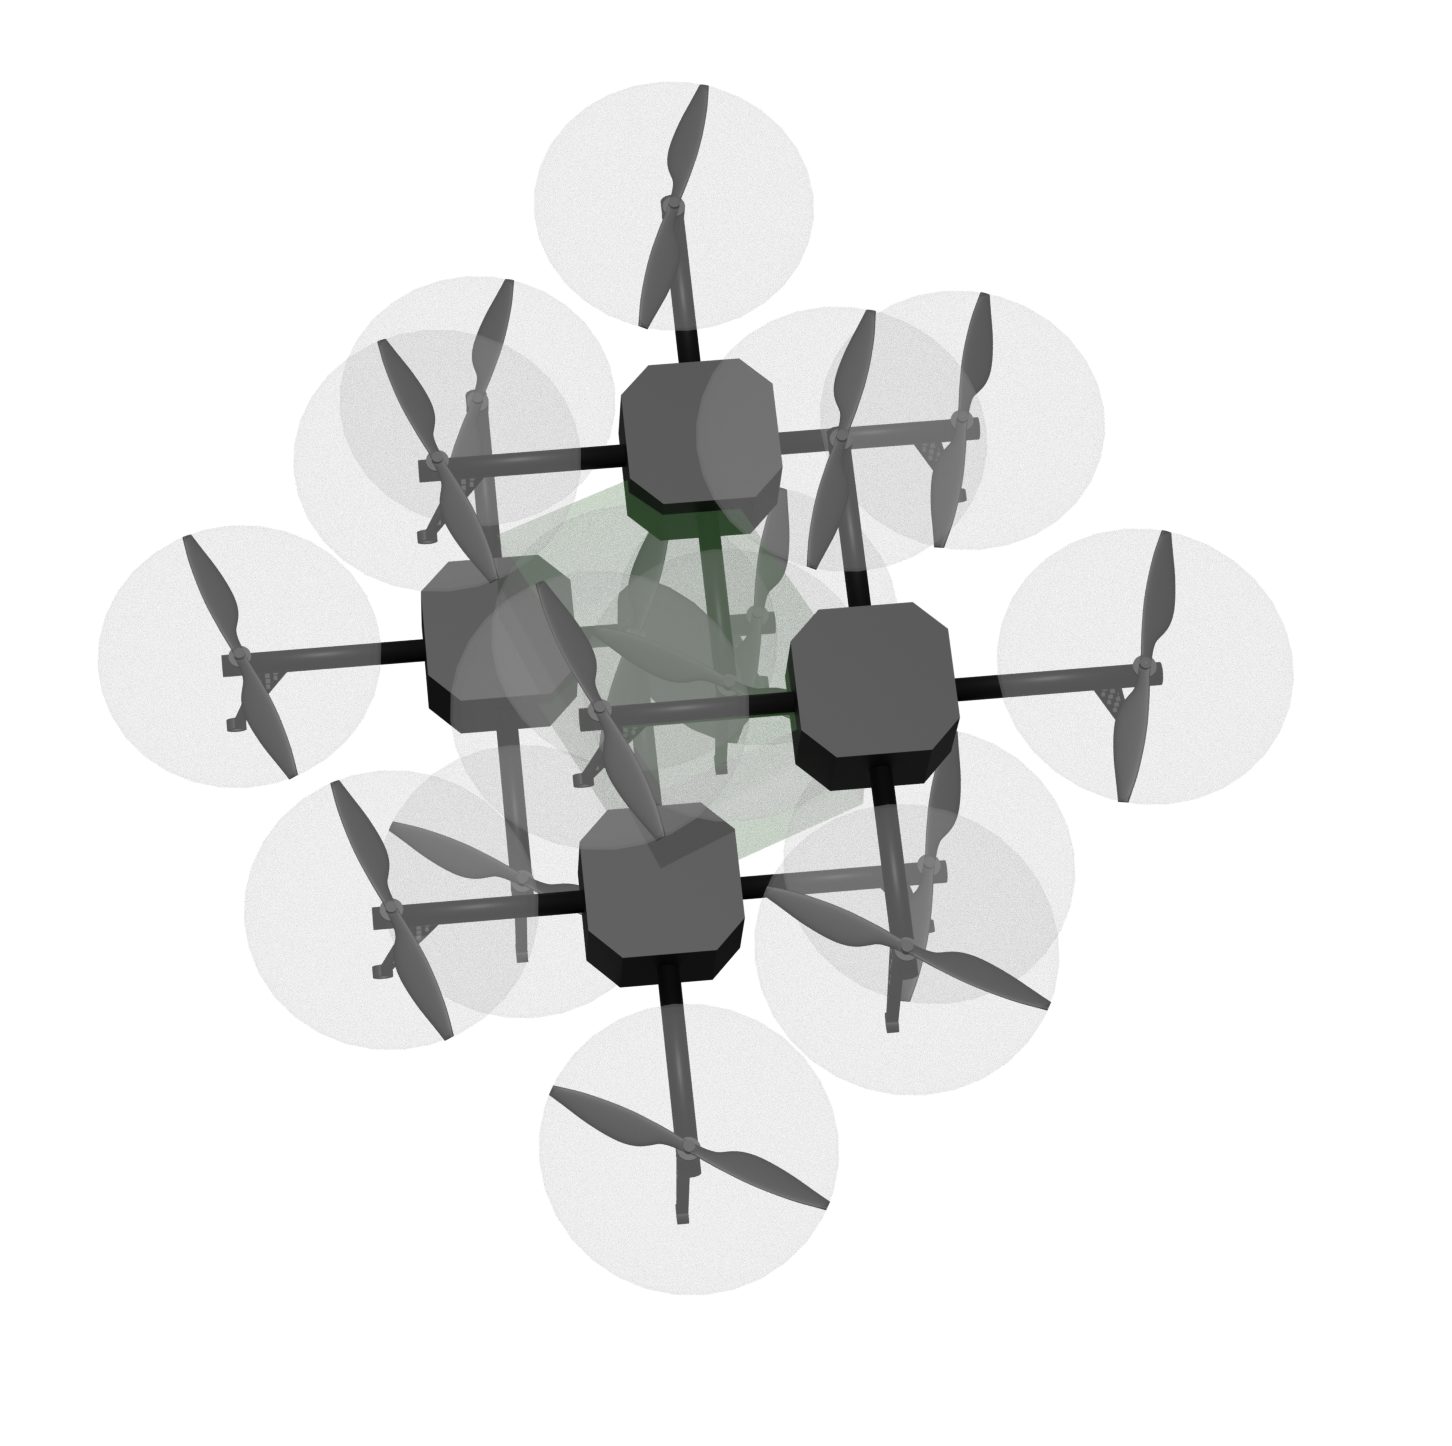
\includegraphics[width=\linewidth]{figures/appendix/CCdrone2.png}
        \caption{}
        \vspace{-0.3cm}
        \label{fig:CCall}
    \end{subfigure}

    \caption{Figure showing the resulting shapes tested for collisions: (a) differential drive robot extended AABB, 
    (b) sampling-based approximated uncertain mesh, for a differential drive robot with its associated uncertainty ellipsoid bounding box (green), (c) quadrotor extended AABB, and (d)
    sampling-based approximated uncertain mesh, for a quadrotor with its associated uncertainty ellipsoid bounding box (green).
    Note that not all the sampled configurations are displayed for clarity.}
    \label{fig:CCmethods}
\end{figure}

Although the methods employed in this thesis for robust collision checking rely on the uncertainty ellipsoid bounding box computed using Equation~\ref{eq:radius}, the tubes are represented by ellipsoids in the various figures of this manuscript for smoother visualization.

\paragraph{Robust saturation checking}
Then, in this manuscript, the feasibility check is not restricted to the aforementioned collision test, but it also verifies that the robot control inputs does not saturate.
This test is performed by checking that the tube associated with each control input remains in its feasibility domain.
An example of infeasible input for the quadrotor case is presented in Figure~\ref{fig:invalid_inputs}, where the tube (green) around the nominal control input of the first actuator (blue) exceeds the maximum allowed input (red).
Note that this simple test is less costly than the robust collision checking one, it is therefore performed first by mean of computational efficiency. 

\begin{figure} [htp]
    \centering
    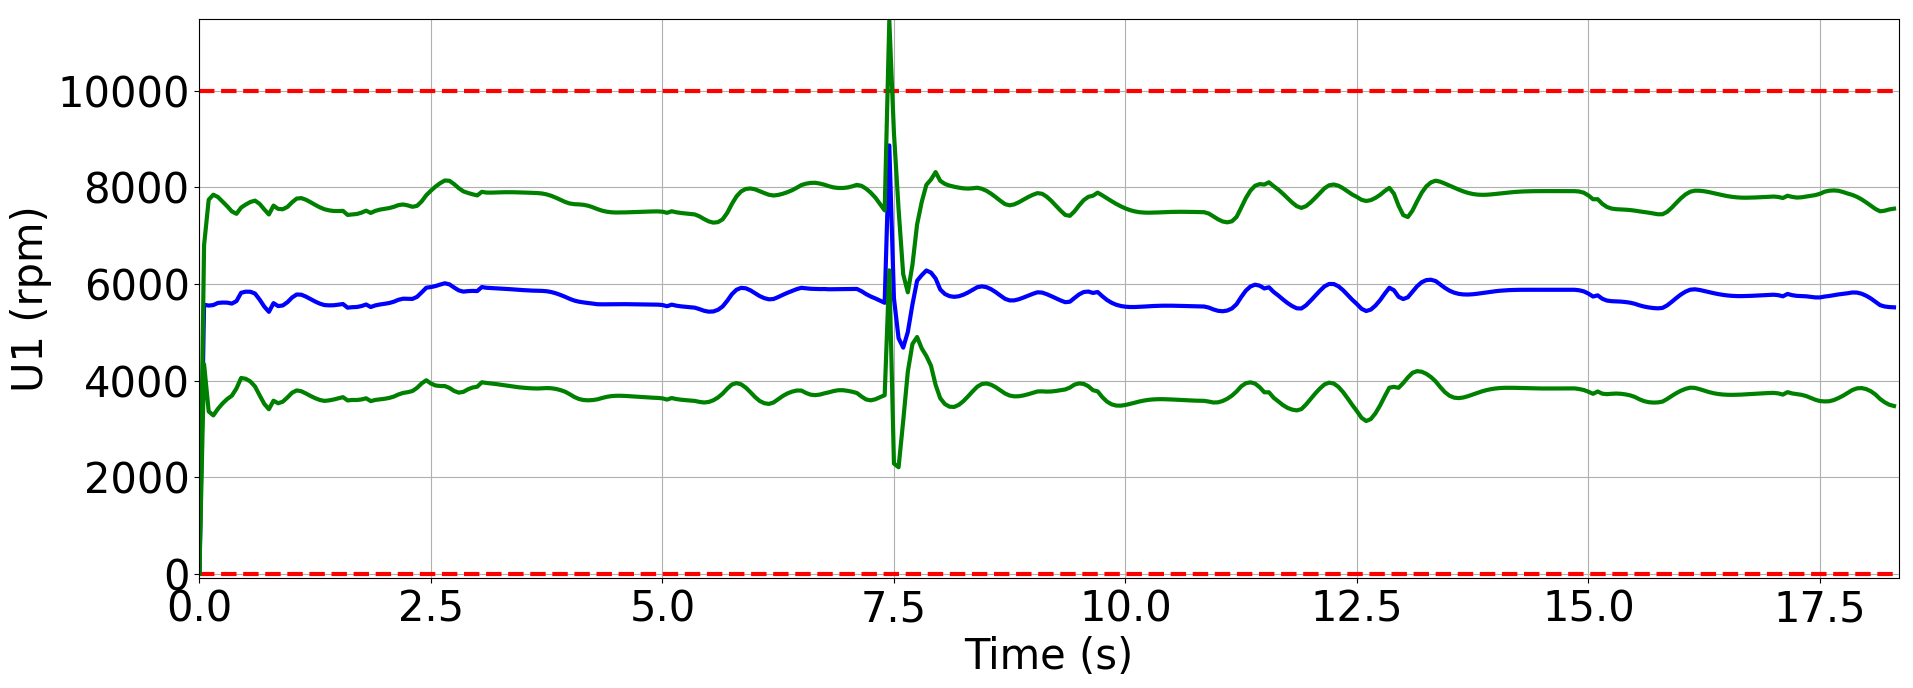
\includegraphics[width=0.8\linewidth]{figures/samp/Invalid_Inputs.png} 
    \caption{Non-robust nominal control input profile for the first rotor of a quadrotor (blue) along a specified trajectory, depicted with its uncertainty tube (green) and the control input limits (red).}%
    \label{fig:invalid_inputs}%
\end{figure}
% \cleardoublepage
% \newpage 
% \ % The empty page
% \newpage
\chapter{Learning curves}\label{chap:appendixB}

\begin{figure} [h]
    \centering
    \vspace{-0.2cm}
    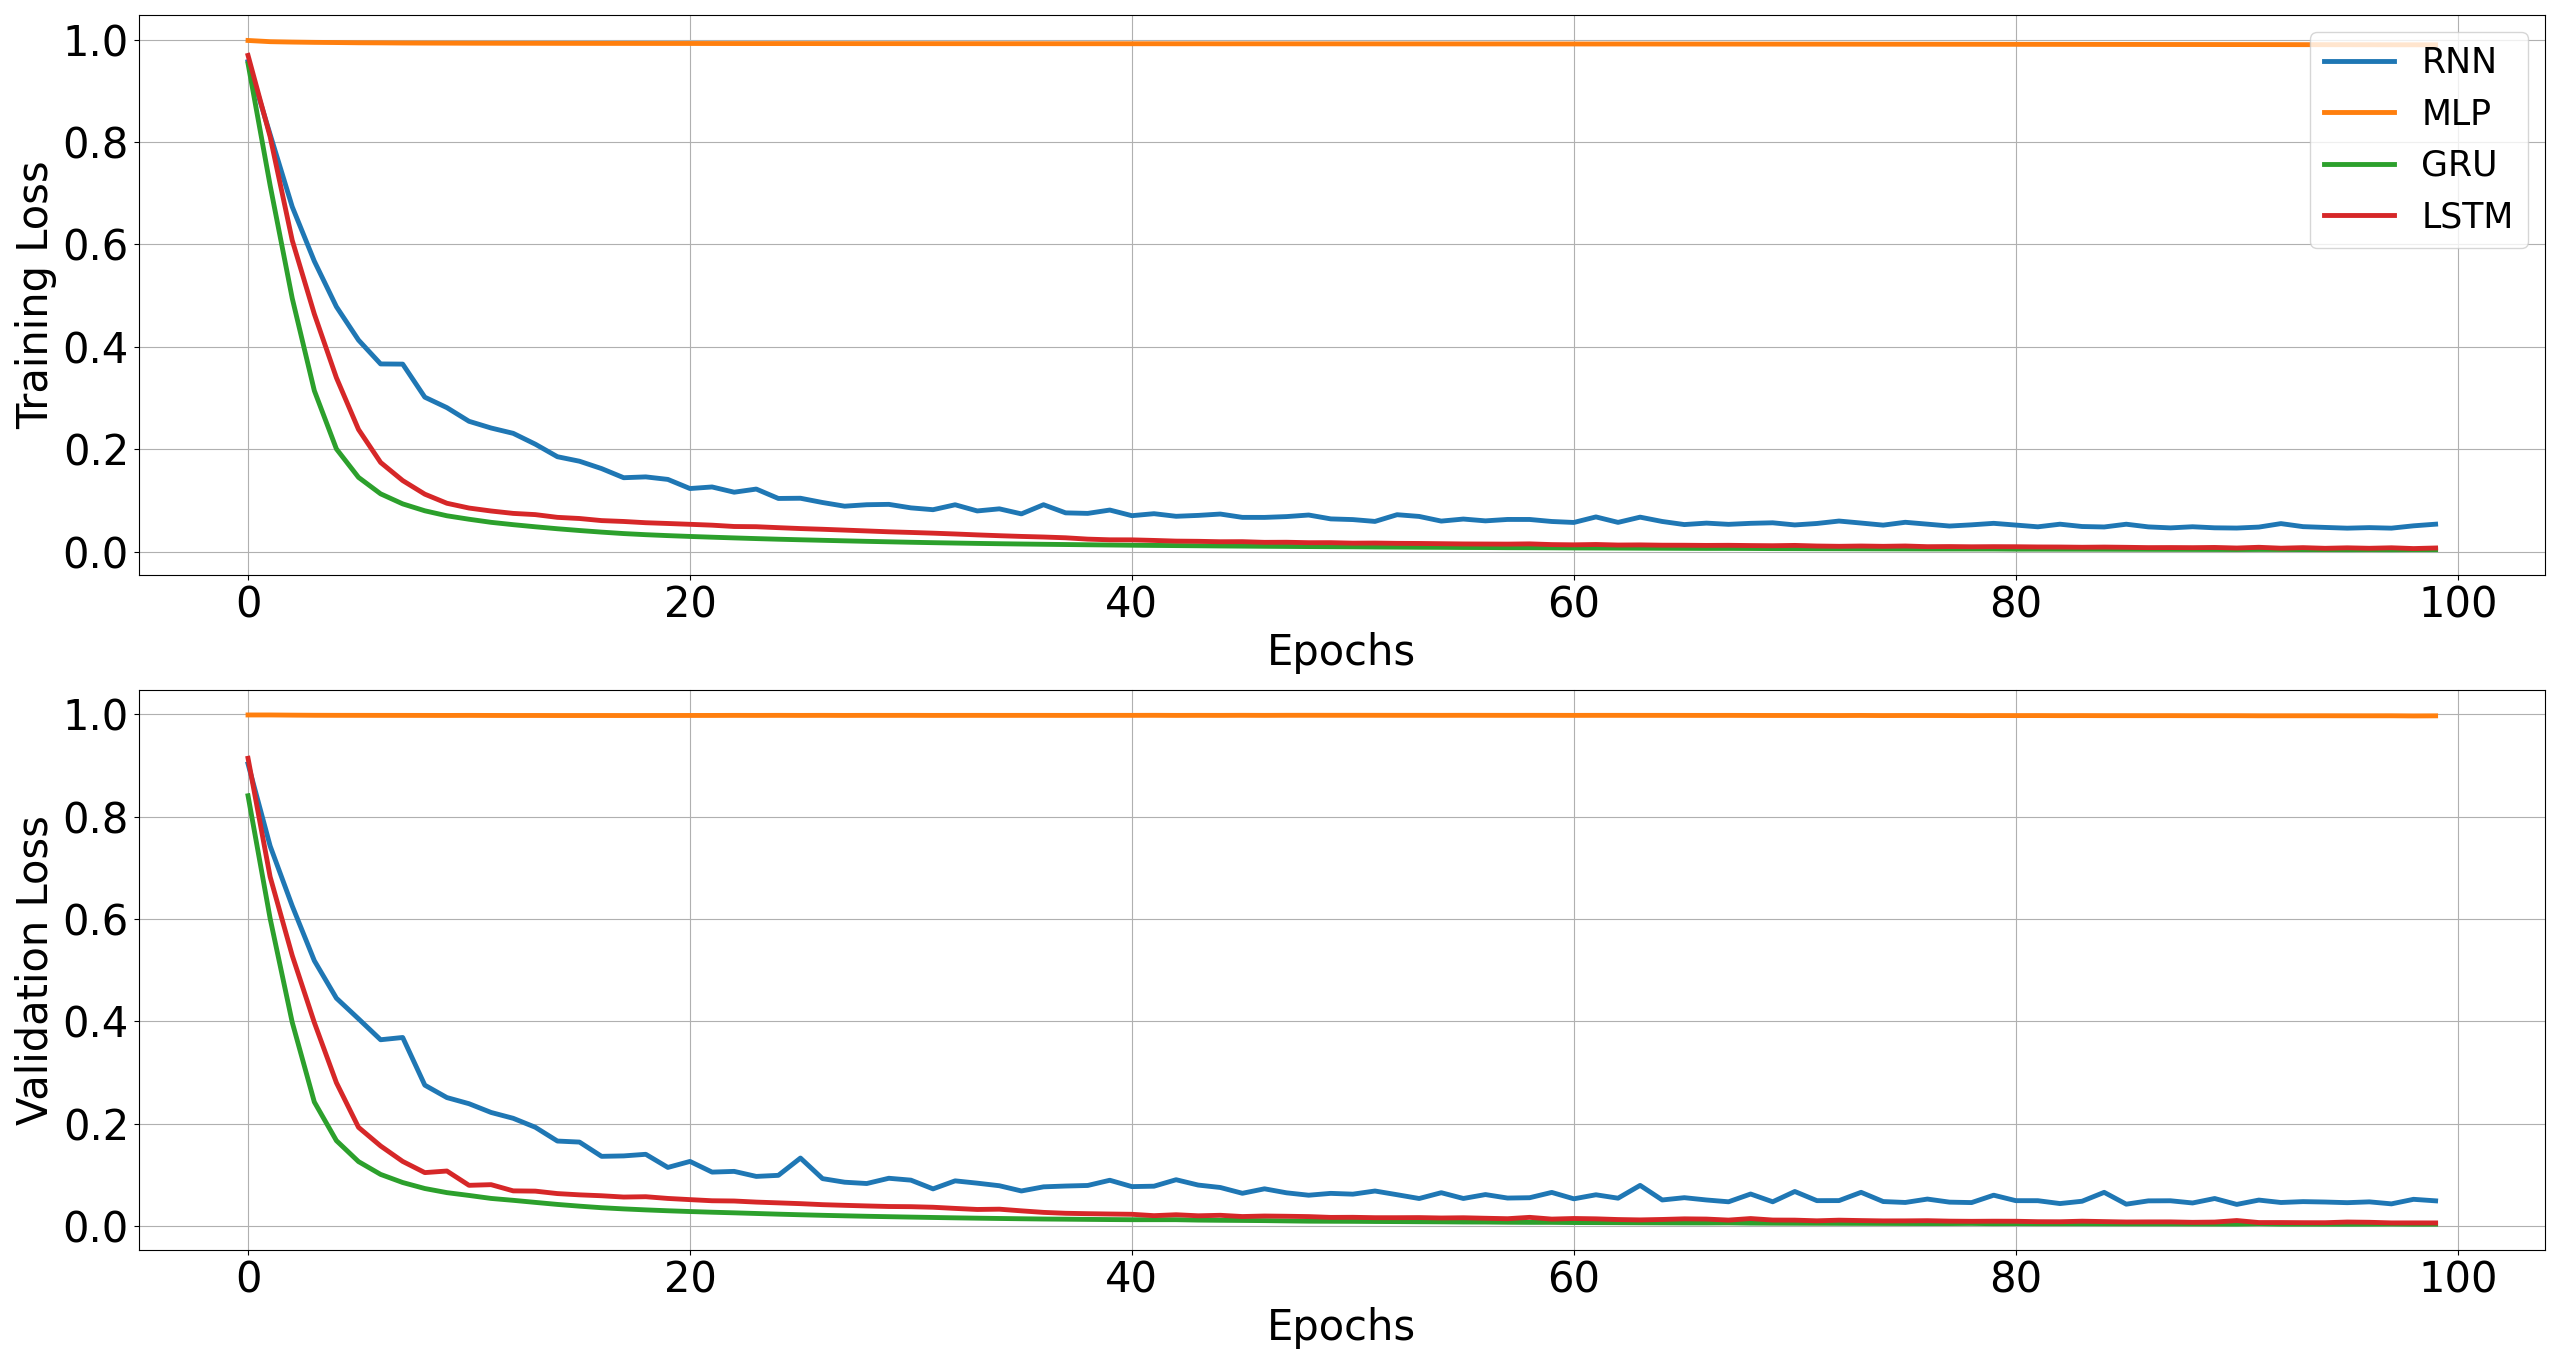
\includegraphics[width=0.95\linewidth]{figures/learning_unic/learning_curves.png}
    \caption{Learning curves showing the evolution of training loss (top) and corresponding validation loss (bottom) for the differential drive robot application.}
    \label{fig:appendix_B_unic}
\end{figure}

\begin{figure} [h]
    \centering
    \vspace{-1cm}
    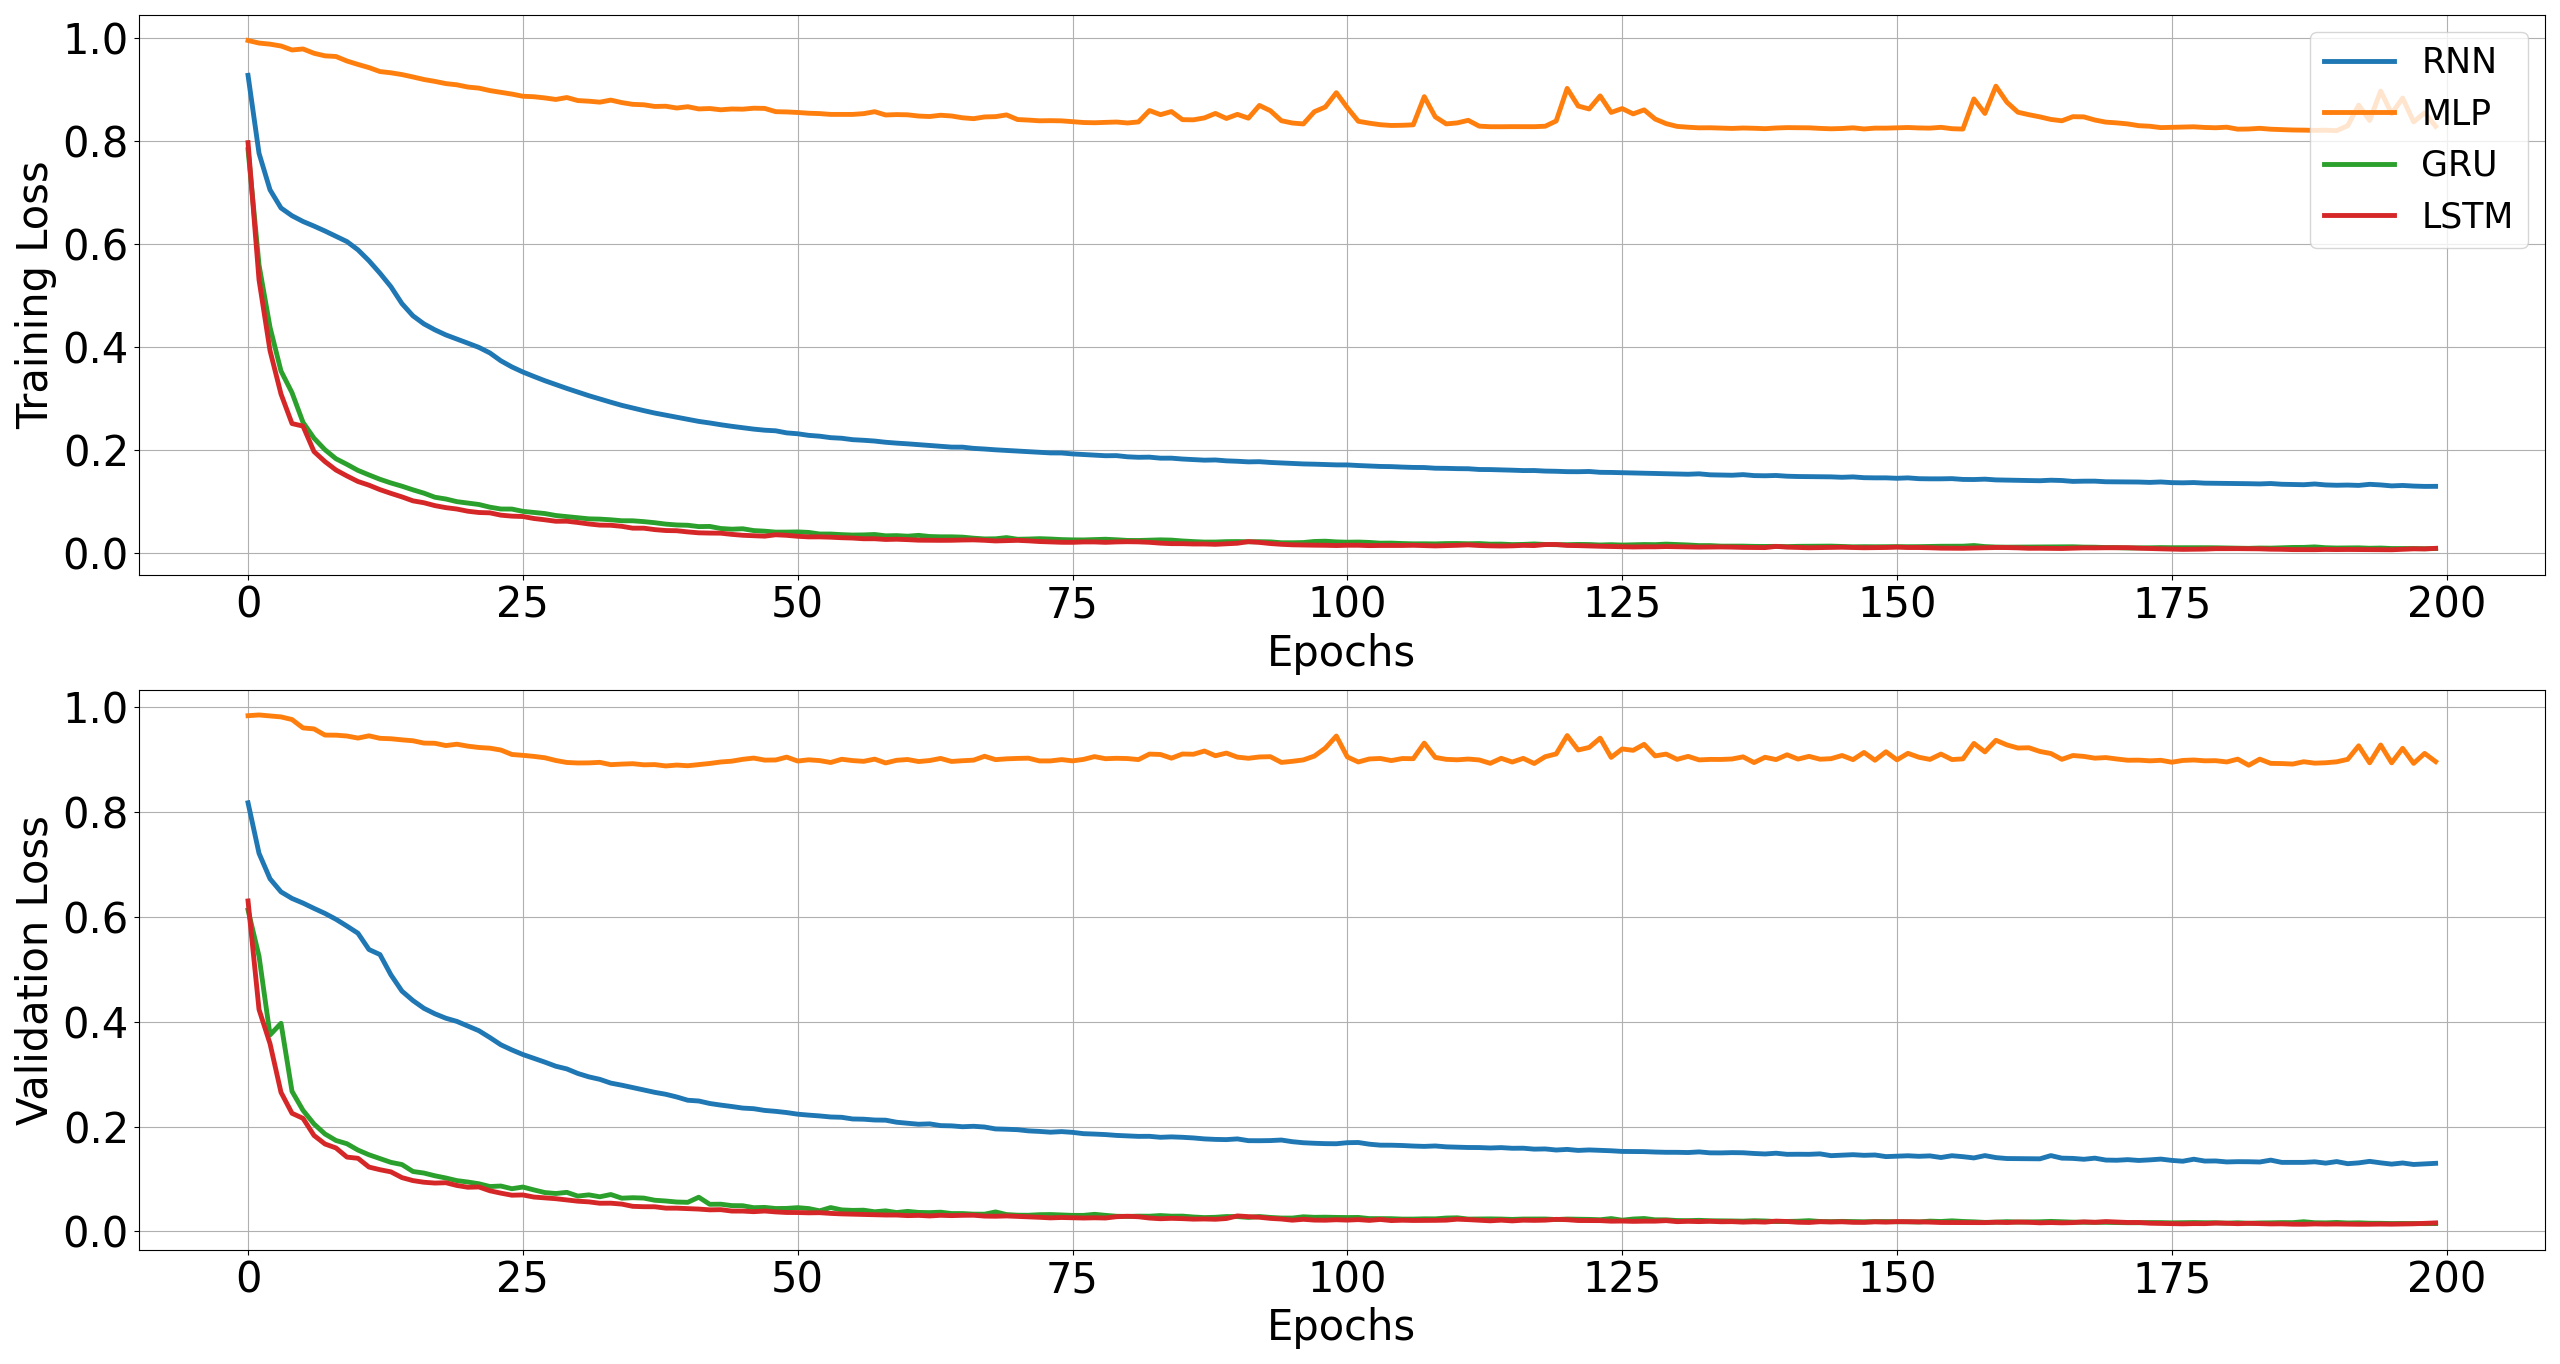
\includegraphics[width=0.95\linewidth]{figures/learning_quadrotor/learning_curves.png}
    \caption{Learning curves showing the evolution of training loss (top) and corresponding validation loss (bottom) for the quadrotor application.}
    \label{fig:appendix_B_quad}
\end{figure}
% \cleardoublepage
% \newpage 
% \ % The empty page
% \newpage
\chapter{ExtendedShortcut}\label{chap:appendixC}

This appendix provides grid search results to determine the optimal hyperparameters for the \myglsentry{saextendedshct} algorithm.

\begin{figure} [htp]
    \centering
    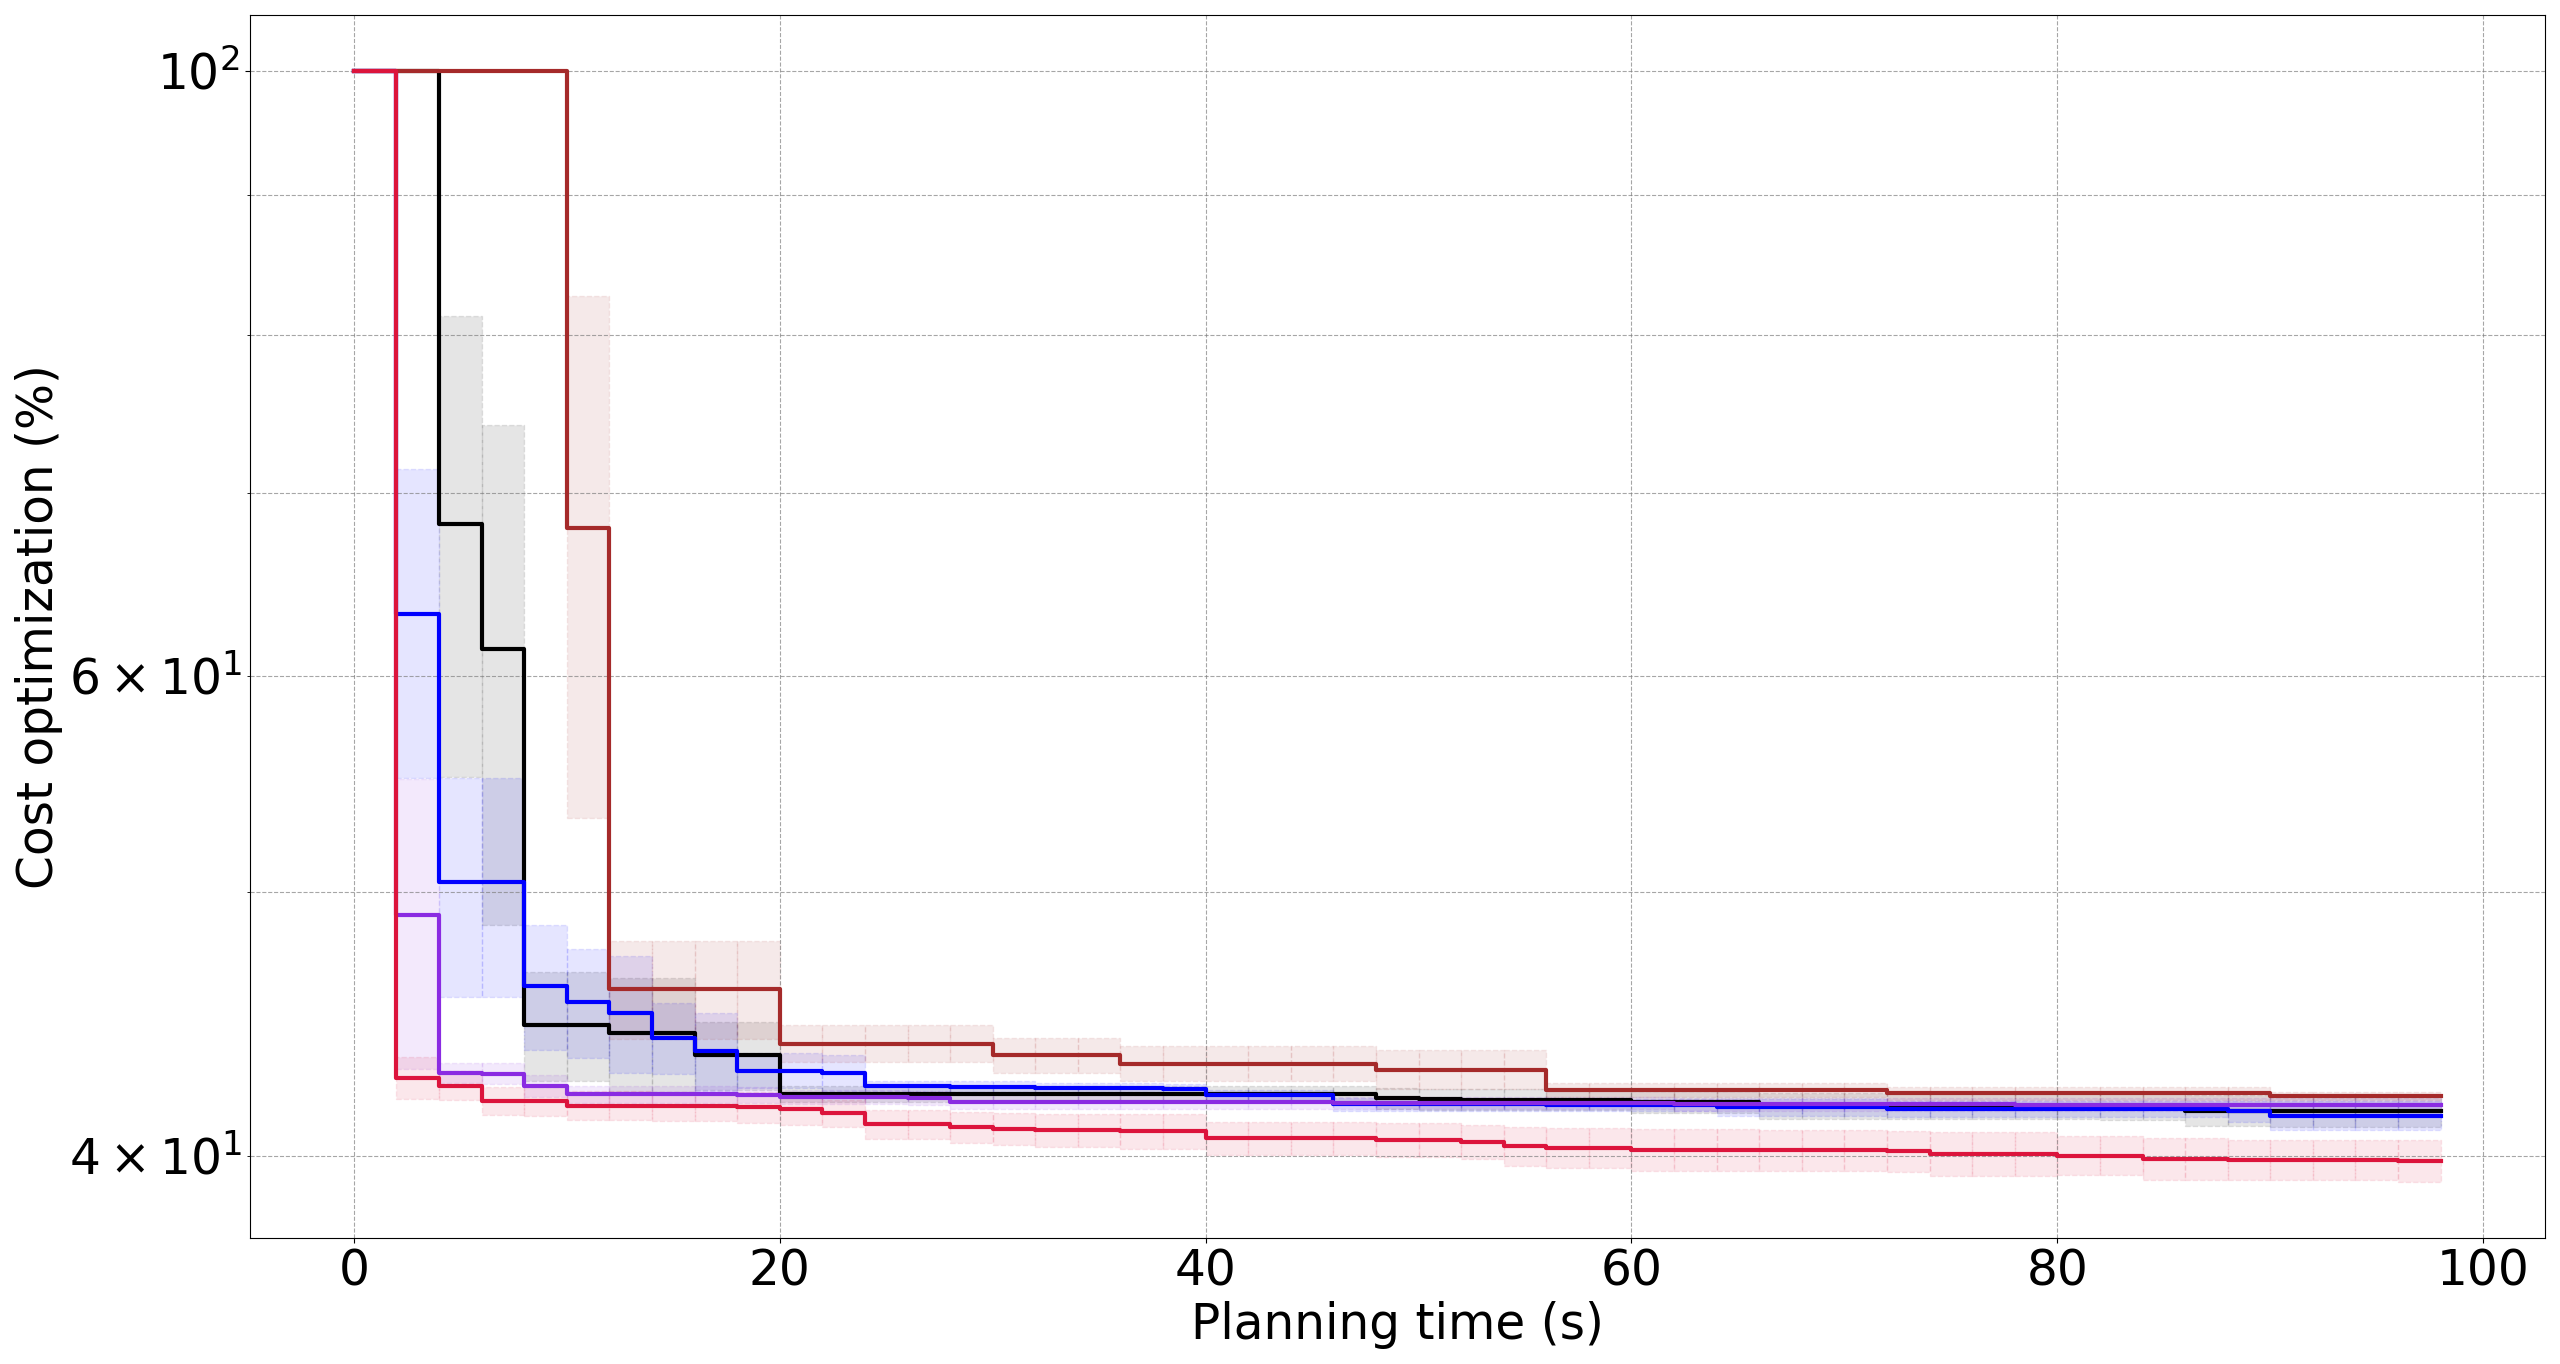
\includegraphics[width=0.9\linewidth]{figures/appendix/uniform_radius_0_01.png} \\
    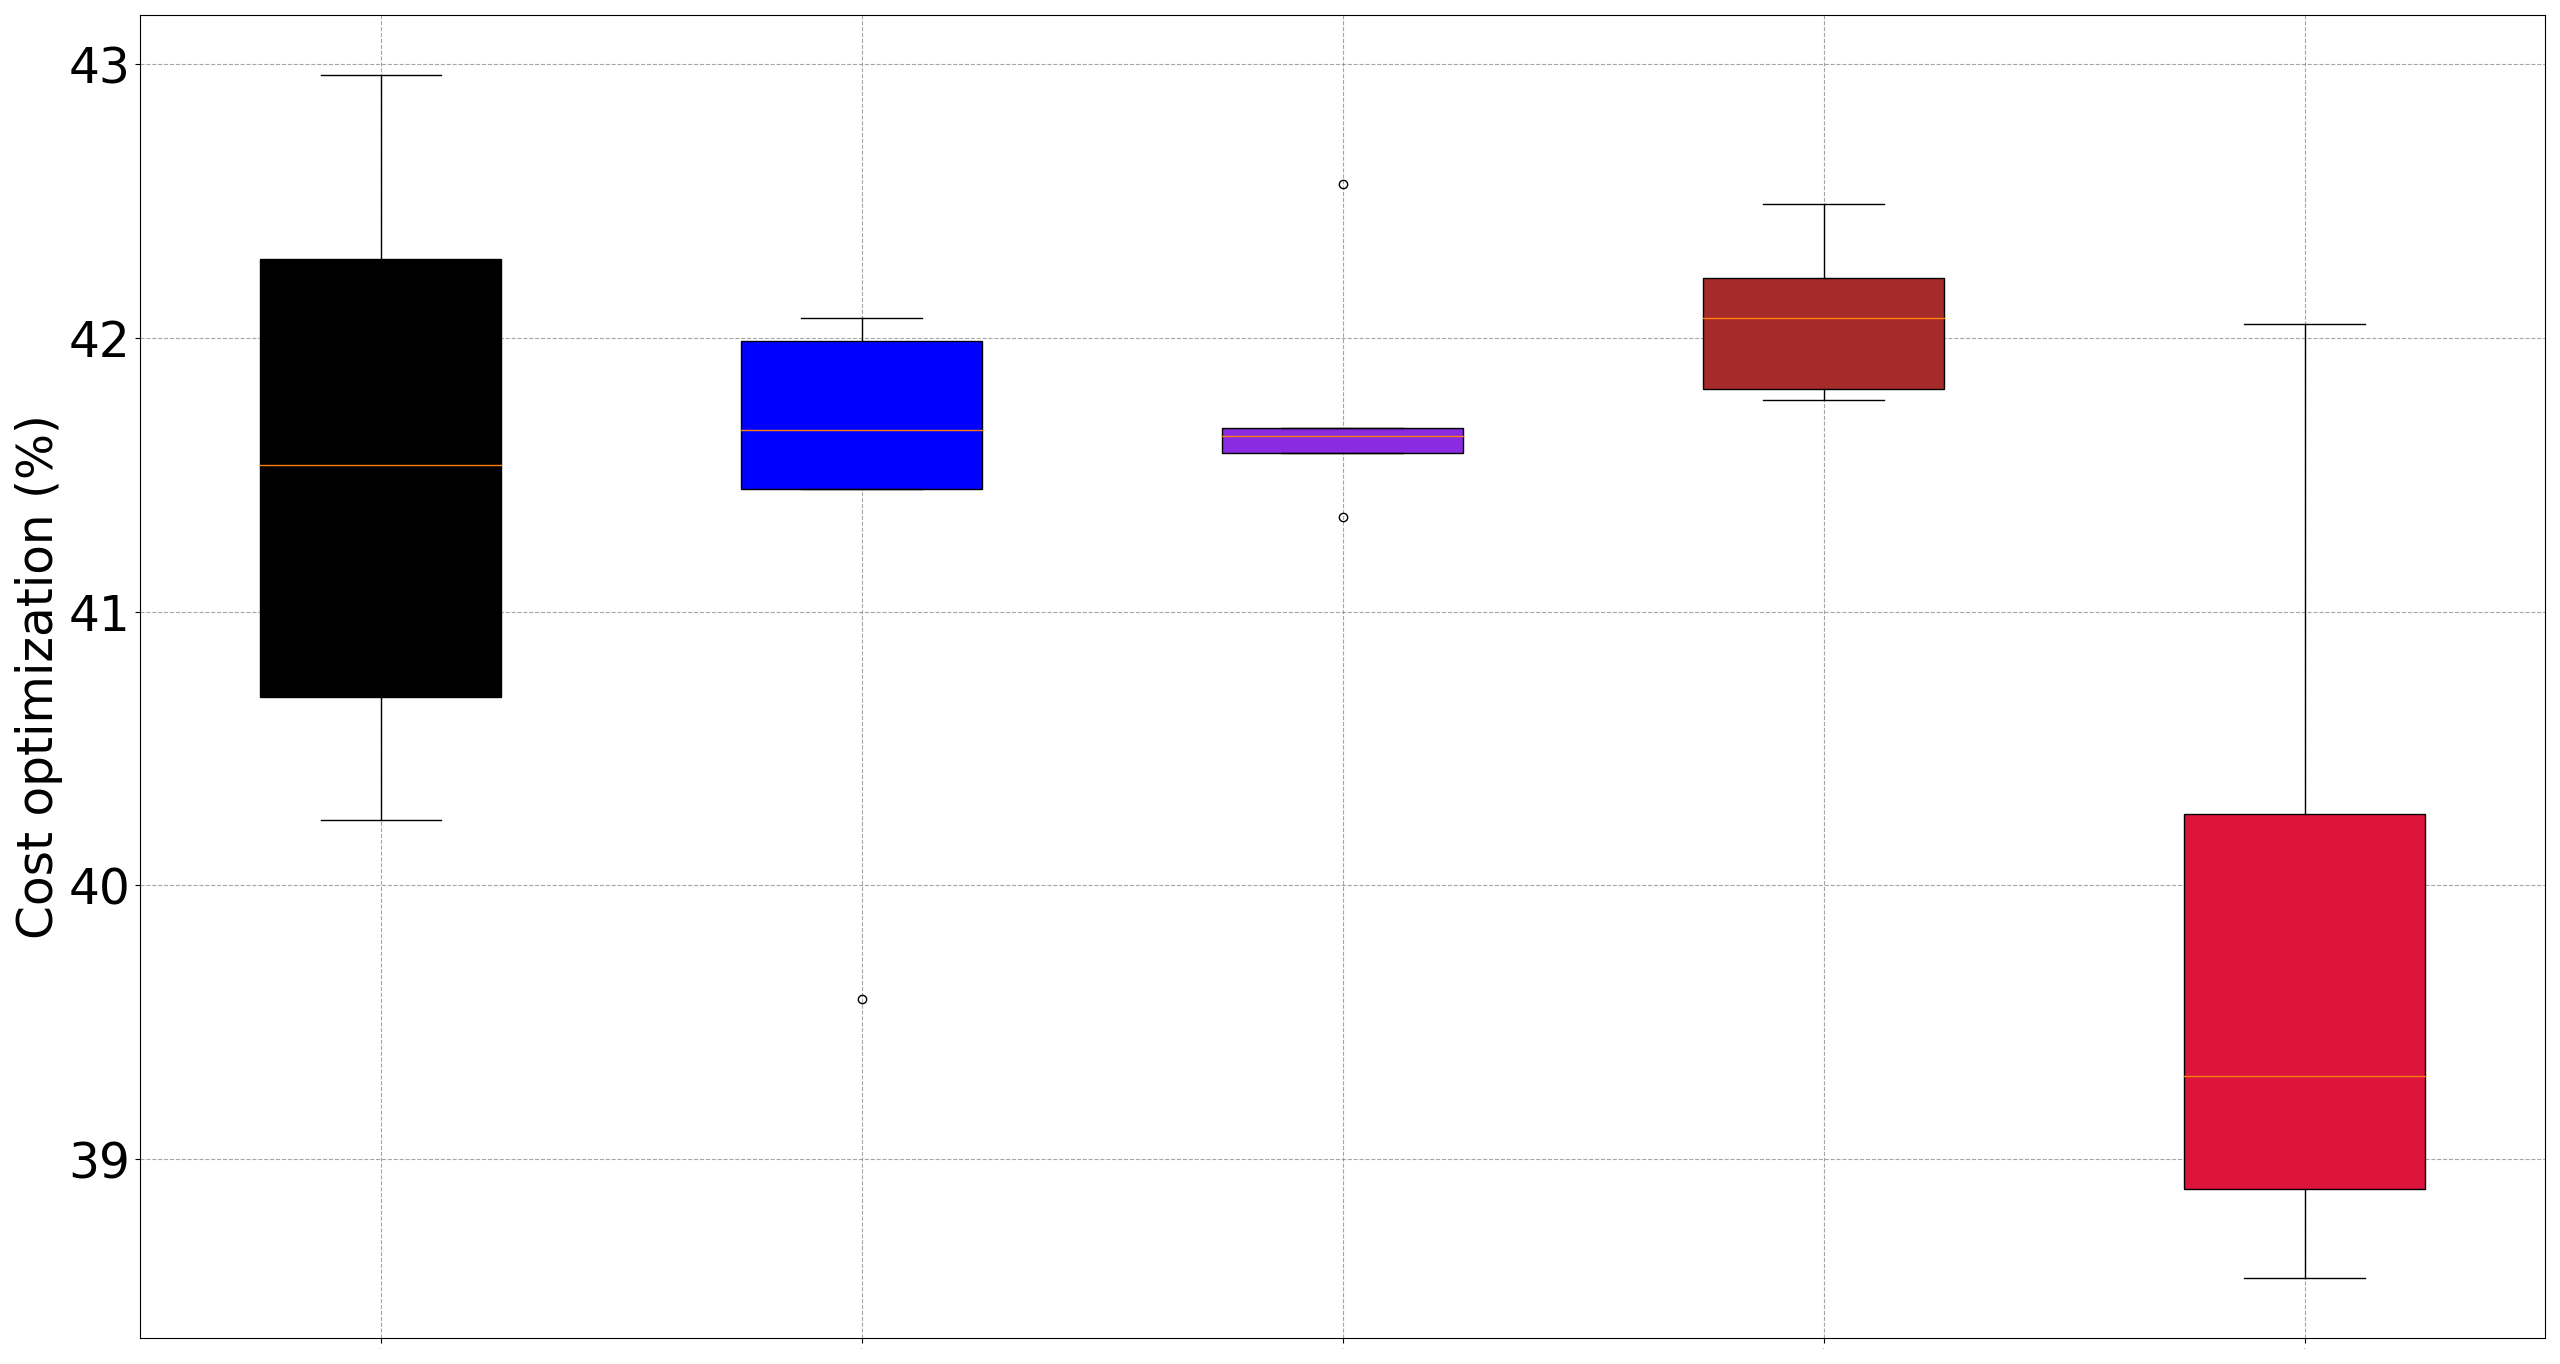
\includegraphics[width=0.9\linewidth]{figures/appendix/bplot_uniform_radius_0_01.png}
    \caption{Cost optimization results using a uniform sampling and a radius $\delta = 0.01$, averaged over 10 plans in a free space environment. 
    The standard deviation is represented as an envelope around the mean curves.
    The red curve corresponds to $K = 1$, the purple curve to $K = 2$, the blue one to $K = 3$, the black to $K = 5$, and the brown curve to $K = 10$.}%
    \label{fig:uniform_radius_0_01}%
\end{figure}

\begin{figure} [htp]
    \centering
    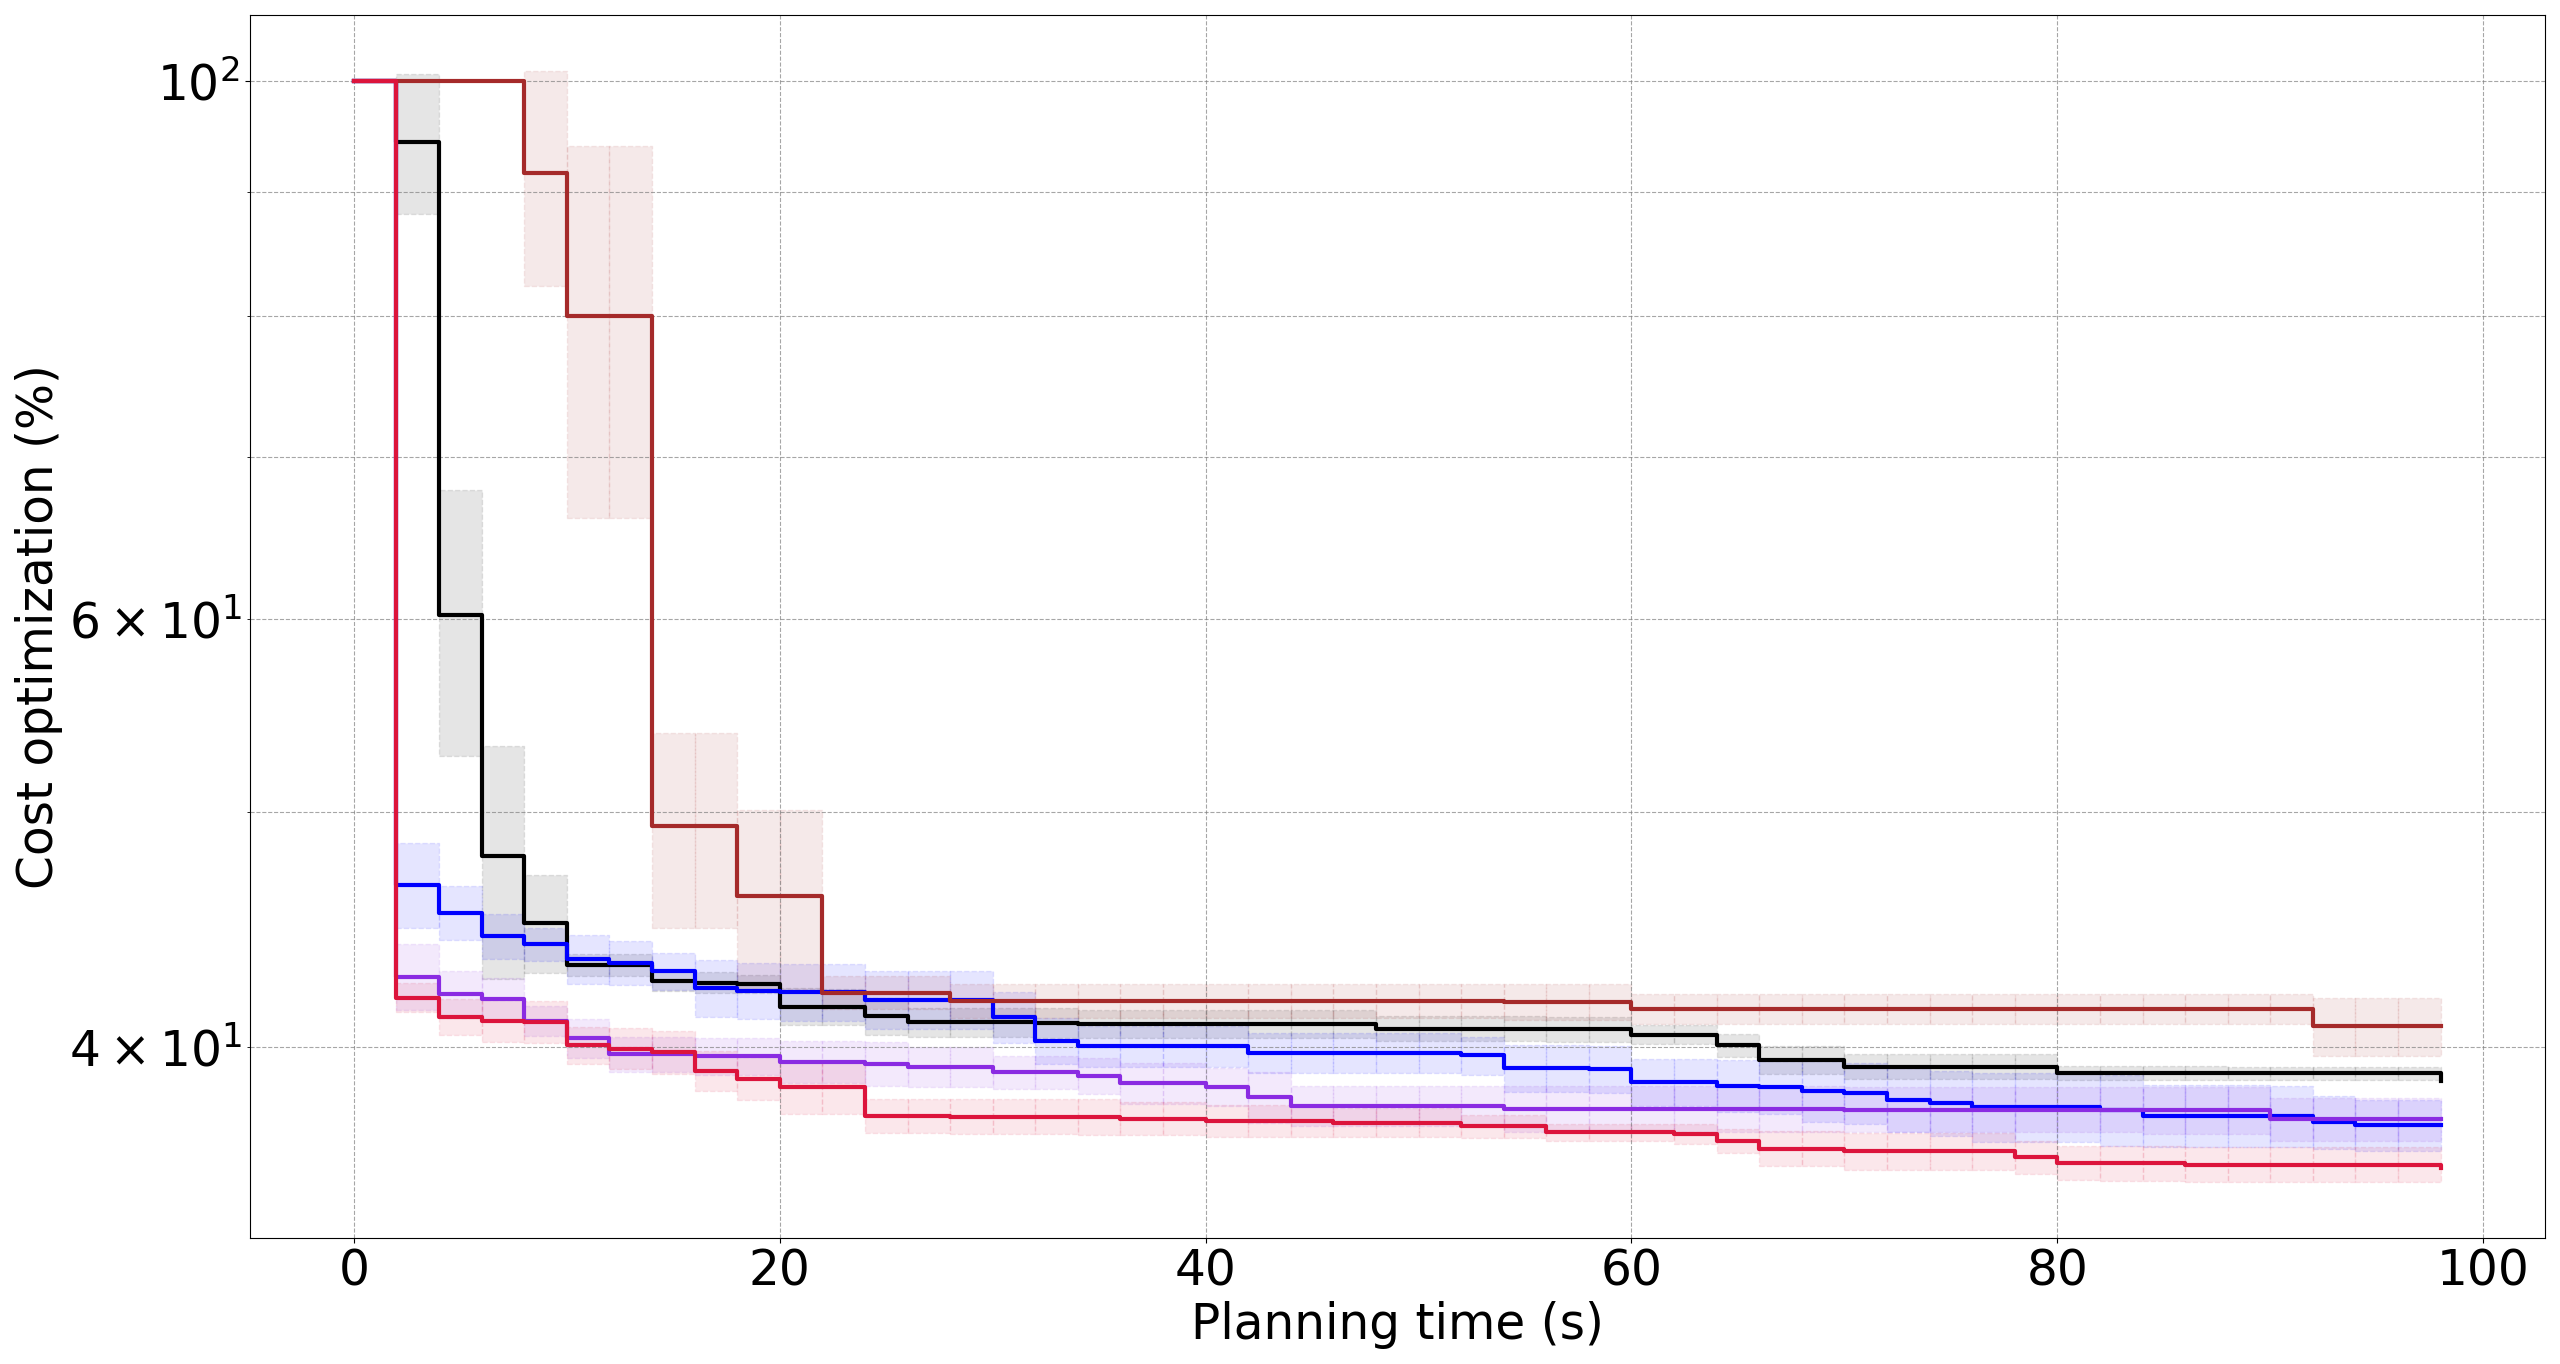
\includegraphics[width=0.9\linewidth]{figures/appendix/uniform_radius_0_1.png} \\
    \includegraphics[width=0.9\linewidth]{figures/appendix/bplot_uniform_radius_0_1.png}
    \caption{Cost optimization results using a uniform sampling and a radius $\delta = 0.1$, averaged over 10 plans in a free space environment. 
    The standard deviation is represented as an envelope around the mean curves.
    The red curve corresponds to $K = 1$, the purple curve to $K = 2$, the blue one to $K = 3$, the black to $K = 5$, and the brown curve to $K = 10$.}%
    \label{fig:uniform_radius_0_1}%
\end{figure}

\begin{figure} [htp]
    \centering
    \includegraphics[width=0.9\linewidth]{figures/appendix/gaussian_radius_0_01.png} \\
    \includegraphics[width=0.9\linewidth]{figures/appendix/bplot_gaussian_radius_0_01.png}
    \caption{Cost optimization results using a Gaussian sampling with a standard deviation $\delta = 0.01$, averaged over 10 plans in a free space environment. 
    The standard deviation is represented as an envelope around the mean curves.
    The red curve corresponds to $K = 1$, the purple curve to $K = 2$, the blue one to $K = 3$, the black to $K = 5$, and the brown curve to $K = 10$.}%
    \label{fig:gaussian_radius_0_01}%
\end{figure}

\begin{figure} [htp]
    \centering
    \includegraphics[width=0.9\linewidth]{figures/appendix/gaussian_radius_0_1.png} \\
    \includegraphics[width=0.9\linewidth]{figures/appendix/bplot_gaussian_radius_0_1.png}
    \caption{Cost optimization results using a Gaussian sampling with a standard deviation $\delta = 0.1$, averaged over 10 plans in a free space environment. 
    The standard deviation is represented as an envelope around the mean curves.
    The red curve corresponds to $K = 1$, the purple curve to $K = 2$, the blue one to $K = 3$, the black to $K = 5$, and the brown curve to $K = 10$.}%
    \label{fig:gaussian_radius_0_1}%
\end{figure}

\begin{figure} [htp]
    \centering
    \includegraphics[width=0.9\linewidth]{figures/appendix/comp.png} \\
    \includegraphics[width=0.9\linewidth]{figures/appendix/bplot_comp.png}
    \caption{Comparison of the best cases found in their respective classes: The red curve corresponds to a Gaussian sampling with $K = 1$ and $\delta = 0.1$, the blue curve is also associated to a Gaussian sampling with $K = 1$ and $\delta = 0.01$.
    The cases using uniform sampling are represented by the black and purple curves, both achieved with $K = 1$, and $\delta = 0.01$ and $\delta = 0.1$ respectively.}%
    \label{fig:comp}%
\end{figure}
% \cleardoublepage
% \newpage 
% \ % The empty page
% \newpage
\chapter{Résumé en Français}
\label{app:fr_small}

La planification du mouvement des robots est essentielle pour garantir un comportement robotique à la fois efficace et sûr.
Cependant, les robots opérant dans des environnements réels font inévitablement face à des incertitudes, qu'il s'agisse de perturbations externes (e.g. le vent), d'inexactitudes dans les modèles, ou d'erreurs d'estimation d'état.
Une approche efficace pour gérer la complexité d'évoluer and présences de ces incertitudes repose sur le paradigme de la "prévision/rétroaction" ou "planification/contrôle". 
Ce processus se déroule en deux étapes principales :
\begin{enumerate}
    \item Phase de Planification (Prévision) : Une trajectoire de référence pour les états et commandes du robot est planifiée en se basant sur les informations disponibles, telles que les modèles du robot et de son environnement. 
    Cette étape, généralement réalisée hors ligne, intègre des contraintes (e.g. évitement de collisions, limitations des actionneurs) et optimise des métriques comme la longueur de la trajectoire ou l'efficacité énergétique. 
    Cependant, une exécution en boucle ouverte de cette trajectoire planifiée échoue souvent en pratique en raison des incertitudes qui affectent les références prévues.
    \item Phase de Contrôle (Rétroaction) : Pour garantir une exécution robuste, un contrôleur de mouvement est employé pour fermer la boucle entre le mouvement planifié et le mouvement réel. 
    Ce contrôleur compense les effets imprévus et les incertitudes qui n'ont pas été prises en compte lors de la planification.
\end{enumerate} 

Bien que cette approche séquentielle séparant planification et contrôle soit efficace, elle présente des limitations significatives :

\begin{itemize}
    \item Les planificateurs modernes excellent à générer des trajectoires réalisables et globalement optimales pour des systèmes à haute dimension et des contraintes complexes. 
    Cependant, ils ignorent généralement le rôle du contrôleur en temps réel, ce qui entraîne deux problèmes majeurs : (1) le contrôleur doit s’écarter de la trajectoire planifiée pour gérer les incertitudes et perturbations, compromettant ainsi rapidement la faisabilité et l’optimalité ; 
    (2) le planificateur ne tient pas compte de la robustesse intrinsèque offerte par le contrôleur, manquant ainsi des opportunités pour produire des plans de mouvement plus robustes.
    \item De nombreuses méthodes de contrôle adaptatif ou robuste (par exemple, H-infini, méthodes LPV) ont été conçues pour gérer efficacement les incertitudes et perturbations, mais elles sont souvent locales vis à vis de la trajectoire de référence. 
    Ces méthodes peinent à relever des défis plus larges comme la faisabilité sous contraintes, l’optimalité globale et les performances, qui sont mieux gérés par des approches de planification globale.
\end{itemize}
    
Pour combler l’écart entre ces deux communautés, plusieurs approches ont été introduites, notamment des contrôleurs plus globaux tels que le \gls{mpc}~\cite{cTMPC}. 
De plus, la dernière décennie a vu émerger le concept de "planification de mouvement avec rétroaction" (feedback motion planning)~\cite{cTognon, cContractThMP, cContractThOnlineMP, cMajundarLibrary, cFaSTrack, cRandUpRRT, cRandUP}. 
Cependant, ces méthodes continuent de rencontrer des défis en termes de généralisabilité, d'efficacité en temps de calcul et de dépendance à des modèles potentiellement inexacts de la pair robot/contrôleur en raison des incertitudes sur les paramètres du modèle.

Ainsi, ce travail, basé sur le paradigme de "planification de mouvement avec rétroaction" (ou "planification de mouvement consciente du contrôle"), exploite le concept de sensibilité en boucle fermée~\cite{cPi,cTh} (une extension de la notion de sensibilité qui incorpore le comportement du contrôleur vis-à-vis des incertitudes paramétriques) afin de créer des planificateurs robustes et conscients du contrôle pour une large classe de systèmes et de contrôleurs, tout en abordant les incertitudes dans leurs représentations modélisées.

Cette thèse débute par une revue de la littérature au Chapitre~\ref{chap:related_work}, qui fournit un aperçu de l’état de l’art. 
Elle se concentre d’abord sur les approches découplées pour la planification robuste de mouvement, en commençant par les méthodes de recherche de chemin et en progressant vers la planification kinodynamique de trajectoire associée à des stratégies de contrôle robuste. 
La revue se poursuit avec des approches unifiées, présentant des méthodes de planification de mouvement robustes prenant en compte les incertitudes, ainsi que des techniques de planification consciente du contrôle. 
Le chapitre se termine par une mise en avant des approches unifiées et robustes conscientes du contrôle, qui constituent le sujet principal de cette thèse.

Les chapitres suivants explorent en détail les contributions principales de cette thèse, depuis l’introduction des concepts de sensibilité en boucle fermée jusqu’à leur application pratique via des planificateurs conscients du contrôle optimisés par apprentissage profond, démontrant leur efficacité dans des scénarios exigeant robustesse et précision élevées.

Le chapitre~\ref{chap:samp} a présenté l'intégration du concept de sensibilité en boucle fermée et des tubes d'incertitude correspondants dans un cadre de planification global basé sur l'échantillonnage, répondant ainsi aux limitations des travaux antérieurs qui se concentraient principalement sur la génération locale de trajectoires. 
Cette méthodologie a permis de générer des trajectoires globalement optimales en termes de sensibilité. 
De plus, pour la première fois, les tubes d'incertitude basés sur la sensibilité ont été utilisés comme contraintes robustes dans le processus de planification, à la fois dans les espaces d'état et d'entrée de contrôle.

Bien que le calcul de ces tubes d'incertitude soit peu coûteux, la charge de calcul globale reste élevée en raison du grand nombre de calculs nécessaires dans les applications basées sur l'échantillonnage. 
Pour remédier à cela, une approche découplée s'appuyant sur une stratégie robuste et paresseuse a été explorée, réduisant considérablement les besoins en calcul, en particulier pour des systèmes de complexité croissante.

Dans cette continuité, le chapitre~\ref{chap:NN} a abordé davantage les défis computationnels en exploitant la similarité structurelle entre le système d'\gls{odes} nécessaire au calcul des tubes et les \myglsentry{rnns}. 
Le réseau de neuronne proposé a permis d'établire une corrélation directe entre la trajectoire planifiée et les tubes d'incertitude, éliminant ainsi le besoin de résoudre les ODEs. 
La méthode a impliqué la génération d'un jeu de données basé sur une approche par échantillonnage adaptée à la tâche. 
En utilisant une cellule simple de type \myglsentry{gru}, l'architecture proposée a atteint un compromis efficace entre la précision des prédictions et la vitesse d'inférence, réduisant le temps de calcul d'un ordre de grandeur par rapport aux solveurs d'ODEs traditionnels.

Dans le chapitre~\ref{chap:sampNN}, cette architecture basée sur les GRU a été appliquée pour développer une alternative efficace à la stratégie ponctuelle de vérification robuste des collisions présentée dans le chapitre~\ref{chap:samp}. 
Des variantes de planification conscient de la sensibilité basées sur l'apprentissage profond ont été proposées, démontrant leur efficacité pour générer des trajectoires robustes dans des temps de planification acceptables. 
De plus, alors que le chapitre~\ref{chap:samp} se concentrait principalement sur la minimisation globale de la sensibilité tout au long du mouvement, les méthodes de ce chapitre se sont orientées vers l'optimisation de la précision. 
Les tubes d'incertitude ont été appliqués de manière sélective à des segments spécifiques du mouvement en fonction des exigences de la tâche.

Une campagne de simulation approfondie a permis d'identifier le meilleur optimiseur local pour cette fonction de coût spécifique, en optimisant à la fois les trajectoires et les gains du contrôleur. 
Les méthodes proposées ont été validées expérimentalement dans deux scénarios exigeants: la navigation d'un quadrirotor à travers une fenêtre étroite et la capture en vol d'anneaux nécessitant une grande précision. 
Ces tests ont mis en évidence l'efficacité des méthodes proposés dans un environnement intérieur. 
Cependant, une validation supplémentaire est nécessaire pour évaluer son applicabilité à des systèmes plus complexes, tels que les manipulateurs aériens.
% \cleardoublepage
% \newpage 
% \ % The empty page
% \newpage

\backmatter

\printbibliography[heading=bibintoc,title={References}]
\cleardoublepage


\end{document}
